\documentclass[12pt]{strath_thesis}

\usepackage{apacite}
\usepackage{amsmath}
\usepackage{amsfonts}
\usepackage[mathscr]{eucal}
\usepackage{ifpdf}
\usepackage{multirow}
\usepackage{dcolumn}
\usepackage{eurosym}
\usepackage{rotating}
\usepackage{pdflscape}
\usepackage{paralist}
\usepackage{ifthen}

%\usepackage{pslatex}
%\usepackage{palatino}

% \ifpdf
%   \usepackage[pdftex]{graphicx}
%   \graphicspath{{./pdf/}{./jpg/}}
%   \DeclareGraphicsExtensions{.pdf,.jpg,.png}
% \else
%   \usepackage[dvips]{graphicx}
%   \graphicspath{{./eps/}}
%   \DeclareGraphicsExtensions{.eps}
% \fi

\usepackage[ruled]{algorithm}
\usepackage{algorithmic}

\usepackage{ulem}

\usepackage{tikz}
\usetikzlibrary{arrows,calc}
\usetikzlibrary{shadows}
\usetikzlibrary{decorations,decorations.pathmorphing}
\usetikzlibrary{positioning,shapes}
\tikzset{
>=stealth', % standard arrow tip
help lines/.style={dashed, thick}, % different line styles
axis/.style={<->},
important line/.style={thick},
connection/.style={thick, dotted},
}

% PGF/TikZ sequence diagrams.
\usepackage[underline=true,rounded corners=false]{pgf-umlsd}

\tikzstyle{line}=[-, thick]
\tikzstyle{loadline}=[->,thick,>=stealth']

\tikzstyle{final}=[rectangle, draw, fill=white, text=black, drop shadow,
		text width=3cm, text centered, rounded corners=2pt]
% \tikzstyle{comment}=[rectangle, draw=black, rounded corners, fill=green,
%     drop shadow, text centered, anchor=north, text=white, text width=3cm]
\tikzstyle{genarrow}=[->, >=open triangle 90, thick]


\newcommand{\busbar}[3]{
  \node[rectangle,draw,fill=black,minimum width=#3,minimum height=2pt,inner
  sep=0pt] (#1) at (#2) {};

%  \node[anchor=south west] at (#2) {#1};
}

\newcommand{\vbusbar}[3]{
  \node[rectangle,draw,fill=black,minimum width=2pt,minimum height=#3,inner
  sep=0pt] (#1) at (#2) {};

%  \node[anchor=south west] at (#2) {#1};
}

\newcommand{\sgen}[2]{
  \node[circle,draw,thick,minimum width=6mm] (#1) at (#2) {};
  \draw[thick] ($(#2)-(2mm,0)$) sin ++(1mm,1mm) cos ++(1mm,-1mm)
  sin ++(1mm,-1mm) cos ++(1mm,1mm);
}

\newcommand{\sload}[2]{
  \node[draw,regular polygon,regular polygon sides=3,minimum size=5mm,inner
  sep=0pt,rotate=180] (#1) at (#2) {};
}

% \newcommand{\genset}[2]{
%   \node[circle,draw,thick,minimum width=10mm] (#1) at (#2) {};
%   \draw[thick] ($(#2)-(3mm,0)$) sin ++(1.5mm,1.5mm) cos ++(1.5mm,-1.5mm)
%   sin ++(1.5mm,-1.5mm) cos ++(1.5mm,1.5mm);
% }

\newcommand{\genset}[3]{
  \node[circle,draw,thick,minimum width=6mm,inner sep=0pt,drop
  shadow,fill=white,#3] (#1) at (#2) {};
  \draw[thick] ($(#2)-(2mm,0)$) sin ++(1mm,1mm) cos ++(1mm,-1mm) sin
  ++(1mm,-1mm) cos ++(1mm,1mm); }

\newcommand{\loadd}[2]{
  \node[draw,regular polygon,regular polygon sides=3,minimum size=1cm,
  rotate=180] (#1) at (#2) {};
}

\newcolumntype{d}[1]{D{.}{\cdot}{#1}}
\newcolumntype{.}[1]{D{.}{.}{#1}}

\makeatletter
\newcommand{\rmnum}[1]{\romannumeral #1}
\newcommand{\Rmnum}[1]{\expandafter\@slowromancap\romannumeral #1@}
\makeatother
\newcommand{\abs}[1]{\lvert#1\rvert}
\newcommand{\diag}{\mathop{\mathbf{diag}}}
\newcommand{\matpower}{\textsc{Matpower~}}
\newcommand{\matlab}{Matlab~}
\newcommand{\psat}{\textsc{Psat~}}
\newcommand{\pylon}{\textsc{Pylon~}}
\newcommand{\stable}{$\bullet$}
\newcommand{\unstable}{$\bullet$}
\providecommand{\e}[1]{\ensuremath{\times 10^{#1}}}

% Optional argument for the parenthesis in bordermatrix.
\makeatletter
\newif\if@borderstar
\def\bordermatrix{\@ifnextchar*{%
\@borderstartrue\@bordermatrix@i}{\@borderstarfalse\@bordermatrix@i*}%
}
\def\@bordermatrix@i*{\@ifnextchar[{\@bordermatrix@ii}{\@bordermatrix@ii[()]}}
\def\@bordermatrix@ii[#1]#2{%
\begingroup
\m@th\@tempdima8.75\p@\setbox\z@\vbox{%
\def\cr{\crcr\noalign{\kern 2\p@\global\let\cr\endline }}%
\ialign {$##$\hfil\kern 2\p@\kern\@tempdima & \thinspace %
\hfil $##$\hfil && \quad\hfil $##$\hfil\crcr\omit\strut %
\hfil\crcr\noalign{\kern -\baselineskip}#2\crcr\omit %
\strut\cr}}%
\setbox\tw@\vbox{\unvcopy\z@\global\setbox\@ne\lastbox}%
\setbox\tw@\hbox{\unhbox\@ne\unskip\global\setbox\@ne\lastbox}%
\setbox\tw@\hbox{%
$\kern\wd\@ne\kern -\@tempdima\left\@firstoftwo#1%
\if@borderstar\kern2pt\else\kern -\wd\@ne\fi%
\global\setbox\@ne\vbox{\box\@ne\if@borderstar\else\kern 2\p@\fi}%
\vcenter{\if@borderstar\else\kern -\ht\@ne\fi%
\unvbox\z@\kern-\if@borderstar2\fi\baselineskip}%
\if@borderstar\kern-2\@tempdima\kern2\p@\else\,\fi\right\@secondoftwo#1 $%
}\null \;\vbox{\kern\ht\@ne\box\tw@}%
\endgroup
}
\makeatother

% Remove figures to speed up build.
\newboolean{includefigures}
\setboolean{includefigures}{false}
% Select chapters to build.
\includeonly{
% 	introduction,
%  	background,
%  	related_work,
 	method,
  	results,
  	conclusion,
  	appendix
}

\ifpdf
\pdfinfo{/Author (Richard W. Lincoln)
  		 /Title  (Learning Power Trade)
         /Subject (Electrical Power Engineering)}
\fi

\title{Learning to Trade Power}
%\title{Learning Power Trade}
\author{Richard W. Lincoln}

\pagestyle{plain}

\begin{document}

\maketitle

\setcounter{page}{1}
\pagenumbering{roman}

\declaration

\begin{acknowledgements}
I wish to thank Professor Jim McDonald for giving me the opportunity to study
at The Institute for Energy and Environment and for giving me the freedom
to pursue my own research interests.  I also wish to thank my supervisors,
Professor~Graeme~Burt and Dr~Stuart~Galloway, for their guidance and
 scholarship.  I wish to offer very special thanks to my parents, my big
brother and my little sister for all of their support throughout my PhD.

This thesis makes extensive use of open source software projects developed by
researchers from other institutions.  I wish to thank Dr Ray Zimmerman from
Cornell University for his work on optimal power flow, researchers from the Dalle Molle Institute for
Artificial Intelligence (IDSIA) and the Technical University of Munich for
their work on reinforcement learning algorithms and artificial neural networks
and Charles Gieseler from Iowa State University for his implementation of the
Roth-Erev reinforcement learning method.

This research was funded by the United Kingdom Engineering and Physical
Sciences Research Council through the Supergen Highly Distributed Power
Systems consortium under grant GR/T28836/01.
\end{acknowledgements}

\begin{abstract}
In Electrical Power Engineering, learning algorithms can be used to model
the strategies of electricity market participants.  The objective of this work
is to establish if \textit{policy gradient} reinforcement learning methods can
provide superior participant models than previously applied \textit{value
function based} methods.

% Electricity is an unique commodity.  It must be supplied at the presise moment
% that it is demanded, as there are no practical methods for significant
% levels of storage in most systems.  There are also few options for controlling
% the direction in which power flows around networks, so generation or
% consumption at one point in the system has an effect at all other points.
Supply of electricity involves technology, money, people, natural resources
and the environment.  All of these aspects are changing and electricity market
designs must be suitably researched to ensure that they are fit
for purpose.  In this thesis electricity markets are modelled as non-linear
constrained optimisation problems that are solved with a primal-dual interior
point method.  Policy gradient reinforcement learning algorithms are used to
adjust the parameters of multi-layer feed-forward neural networks that
approximate each market participant's policy for selecting power quantities
and prices that are offered in a simulated marketplace.

Traditional reinforcement learning methods that learn a value function have
been previously applied in simulated electricity trade, but are
largely restricted to discrete representations of a market environment.
Policy gradient methods have been proven to offer convergence guarantees in continuous environments,
such as in robotic control applications, and avoid many of the problems that
mar value function based methods.

% The benefits of using policy gradient methods in electricity market simulation
% are explored and the results demonstrate their superior trading ability when
% operating in large constrained networks.
% By introducing advanced unsupervised learning methods to electricity market
% simulation, previous research in the field may be revisited and enhanced and
% an opportunity to use policy gradient methods in decision support and automated
% energy trading applications is opened.

% Reinforcement learning methods that use connectionist systems for value
% function approximation offer few convergence guarantees, even in simple
% systems.  Table-based value function reinforcement learning methods have been
% used previously for the simulation of electricity markets, but they operate
% only in discrete action and sensor domains.  If learning algorithms are to
% deliver on their potential for application in operational settings then it will
% be necessary for them to operate in continuous domains.  The principle
% contribution of this thesis is the demonstration of policy-gradient
% reinforcement learning algorithms being applied to continuous representations
% of electricity trading problems, showing that superior use of sensor data
% results in improved overall performance when compared with previously applied
% value-function methods.  From this it follows that learning methods which
% search directly in the policy space will be better suited to decision support
% applications and automated electric power trade.
\end{abstract}

\tableofcontents
\newpage

\listoffigures
\addcontentsline{toc}{chapter}{List of Figures}
\newpage

\listoftables
\addcontentsline{toc}{chapter}{List of Tables}
\newpage

\pagenumbering{arabic}
\setcounter{page}{1}

\onehalfspacing

% Set the scene and problem statement. Introduce structure of thesis, state
% contributions (3-5).
\chapter{Introduction}
This thesis examines reinforcement learning algorithms in the domain of
electric power trade.  In this chapter the motivation for research into
electricity trade is explained, the problem under consideration is defined and
the principle research contributions are stated.

\section{Research Motivation}
% \section{Motivation for Electricity Market Research}
Quality of life for a person is directly proportional to his or her electricity
usage \cite{alam:qol}.  The world population is currently 6.7~billion and
forecast to exceed 9~billion by 2050 \cite{un:pop}. Electricity production
currently demands over one third of the annual primary energy extracted
\cite{iea:2010} and as more people endeavour to improve their quality of life,
finite fuel resources will become increasingly scarce. Market mechanisms, such
as auctions, where the final allocation is based upon the claimants' willingness
to pay for the goods, provide a device for efficient allocation of resources in
short supply.  Two decades ago the UK became the first large industrialised
country to introduce competitive markets for electricity generation.

% Commercialisation of large electricity supply industries began two decades ago
% in the UK.
The inability to store electricity, once generated, in a commercially viable
quantity prevents it from being traded as a conventional commodity. Trading
mechanisms must allow shortfalls in electric energy to be purchased at short
notice from quickly dispatchable generators.
% Different market structures that facilitate this have been implemented in
% countries and states around the world.
Designed correctly, a competitive electricity market can promote efficiency and
drive down costs to the consumer, while design errors can quickly allow market
power to be abused and market prices to be elevated. It is essential
to research electricity market architectures and ensure that their unique
designs are fit for purpose.
% Electricity market designs are particularly complicated due to the need to
% manage complex dynamic constraints imposed by electric power systems.

The value of electricity to society makes it impractical to
experiment with radical changes to trading arrangements on real systems.
The average total demand for electricity in the United Kingdom (UK) is
approximately 45GW and the cost of buying 1MW for one hour is around
\pounds40 \cite{decc:dukes09}. This equates to yearly transaction values of
\pounds16 billion.  The value of electricity becomes particularly
apparent when supply fails. The New York black-out in August 2003 involved
a loss of 61.8GW of power supply to approximately 50 million consumers.
The majority of supplies were restored within two days, but the event is
estimated to have cost more than \$6~billion \cite{minkel:2008,icf:2003}.

An alternative approach is to study abstract mathematical models of markets with
sets of appropriate simplifying approximations and assumptions applied.  Market
characteristics can established by simulating the models using digital computer
programs. Competition between participants is a fundamental feature of all
markets, but the strategies of humans can be difficult to model mathematically.
One option is to use reinforcement learning algorithms from the field of
artificial intelligence.  These methods can be used to represent adaptive
behaviour in competing players and, when correctly configured, have been shown
to be capable of learning highly complex strategies \cite{tesauro:gammon}.  This
thesis makes advances in electricity market participant modelling through the
application of a relatively new genre of reinforcement learning methods called
policy gradient algorithms.

\section{Problem Statement}% and Hypothesis}%/Aims \& Objectives}
Individuals participating in an electricity market (be they representing
generating companies, load serving entities, firms of traders etc.)~must utilise
multi-dimensional data to their advantage. This data may be noisy, sparse,
corrupt, have a degree of uncertainty (e.g.~demand forecasts) or be hidden from
the participant (e.g.~competitor bids).  Reinforcement learning algorithms must
be capable of operating with this kind of data if they are to successfully model
participant strategies.

Traditional reinforcement learning methods, such as Q-learning, attempt to find
the \textit{value} of each available action in a given state.  When discrete
state and action spaces are defined, these methods become restricted by
Bellman's Curse of Dimensionality \cite{bellman:1961} and can not be readily
applied to complex problems.  Function approximation techniques, such as
artificial neural networks, can be used with these methods and allow them to be
applied to continuous environment representations. However, value function
approximation has been shown to result in convergence issues, even in simple
problems \cite{tsitsiklis:94,peters:enac,gordon:95,baird:95}.

Policy gradient reinforcement learning methods do not attempt to approximate a
value function, but instead try to approximate a \textit{policy function} that,
given the current perceived state of the environment, returns an action
\cite{petersScholar}. They do not suffer from many of the problems that mar
value function based methods in high-dimensional problems.  They have strong
convergence properties, do not require that all states be continuously visited
and work with state and action spaces that are continuous, discrete or mixed
\cite{peters:enac}.  Policy performance may be degraded by uncertainty in state
data, but the learning methods do not need to be altered.
They have been successfully applied in many operational settings, including:
robotic control \cite{shaal:robots}, financial trading \cite{moody:direct} and
network routing \cite{peshkin:routing} applications.

It is proposed in this thesis that agents which learn using policy gradient
methods may outperform those using value function based methods in simulated
competitive electricity trade.  It is further proposed that policy gradient
methods may operate better under dynamic electric power system conditions,
achieving greater profit by exploiting constraints to their financial benefit.
This thesis will compare value function based and policy gradient learning
methods in the context of electricity trade to explore these proposals.

% Methods including learning classifier systems, genetic algorithms and
% reinforcement learning have been successfully used to research the
% charateristics of energy markets in the past\cite{weidlich:08}.  This an
% alternative to the traditional closed-form equilibrium approaches to game
% theory research in which behavior emerges from the interactions of many
% separable, self-serving agents. Typically in these studies, an agent is
% associated with a portfolio of generating units and/or dispatchable
% loads. Interaction with the environment involves submission of offers to sell
% or bids to buy\footnote{Beware that certain authors may use the term ``bid''
% to refer to an offer to sell when discussing single-sided auctions.} a
% quantity of power at a specified price in a particular time period.  The
% learning algorithms typically use revenue or earnings as a reward signal and
% adjust the policy used to select offer/bid price and quantity values.

% Research into electricity markets using reinforcement learning typically
% involves discretization the action domain, often into incremental markups
% on marginal cost.  Also, either sensor domains are discretized or state
% information is disregarded altogether.  Despite these simplifications, authors
% have been drawn many practical conclusions from this approach \cite{weidlich:08}.
% If learning algorithms are to deliver on their potential for application in
% operational electricity market settings, modelling continuous domains will be
% necessary.

% Traditional reinforcement learning methods such as Sarsa and Q-learning (See
% Section \ref{sec:rl}, below) can be applied to systems with continuous domains
% by using connectionist systems for value function approximation
% \cite{barto:neuron}. However, feedback between policy updates and value
% function changes can result in oscillations or divergence in these algorithms
% even when applied to simple systems \cite{peters:enac}.  In response to this,
% policy-gradient methods, pioneered by Williams \cite{williams:reinforce}, which
% search directly in the policy space have been developed and applied in many
% real-life settings
% \cite{barto:policy,shaal:robots,moody:direct,peshkin:routing}.
%
% The proposal is to combine policy-gradient reinforcement learning methods with
% artificial neural networks for continuous policy function approximation and
% apply to simulations electricity trade.  The hypothesis being that superior use
% of sensor data results in improved performance over previously applied
% value-function methods.

\section{Research Contributions}
The research presented in this thesis pertains to the academic fields of
electrical power engineering, artificial intelligence and economics.  The
principle contributions made by this thesis are:
\begin{enumerate}
  \item The first application of policy gradient reinforcement learning
  methods in simulated electricity trade. A relatively new class of
  unsupervised learning algorithms, designed for operation in multi-dimensional,
  continuous, uncertain and noisy environments, are applied in dynamic
  techo-economic simulations of international significance.
  \item The first application of a non-linear AC optimal power flow formulation
  in agent based electricity market simulation. The constraining assumptions of
  linearised DC models not being applied provides more accurate electric power
  systems models in which reactive power flows and voltage magnitude constraints
  are considered.
  \item A new Stateful Roth-Erev reinforcement learning method for application
  in complex environments with dynamic state.
  \item A comparison of policy gradient and value function based reinforcement
  learning methods in convergence to states of Nash equilibrium. Results from
  published research for value function based methods are reproduced and
  extented to provide a foundation for the application of policy gradient
  methods in more complex electric power trade simulations.
  \item An examination of the exploitation of electric power system constraints
  by policy gradient reinforcement learning methods.  The
  superior multi-dimensional, continuous data handling abilities of policy
  gradient methods are tested by exploring their ability to observe voltage
  constraints and exploit them and achieve increased profits.
  \item The delivery of an extensible open source multi-learning-agent-based
  power exchange auction market simulator for electric power trade research.
  Sharing software code can dramtically accelerate research of this kind and an
  extensive suite of the tools developed for this thesis have been released
  under liberal open source licenses.
  \item The concept of applying Neuro-Fitted Q-Iteration and GQ$(\lambda)$ in
  simulations of competitive energy trade. New unsupervised learning algorithms
  developed for operation in continuous environments could be utilised in
  electric power trade simulation and some of the most promising examples have
  been identified.
%   \item A formulation of optimal power flow as a reinforcement learning
%   problem.
%   \item Capital investment planning formulated as a reinforcement learning
%   problem.
%  \item A model of the UK transmission system derived from data in the
%  National Grid Seven Year Statement.
\end{enumerate}
The publications that have resulted from this thesis are:
%\citeA{lincoln:pyreto,lincoln:eem07,lincoln:upec}.

\vspace{1pc}
Lincoln, R., Galloway, S., \& Burt, G. (2009, May 27-29). Open source,
agent-based energy market simulation with Python. In \ul{Proceedings of
the 6$^{\textrm{th}}$ International Conference on the European Energy Market,
2009. EEM 2009.} (p.~1-5).

\vspace{1pc}
Lincoln, R., Galloway, S., \& Burt, G. (2007, May 23-25). Unit
commitment and system stability under increased penetration of distributed
generation. In \ul{Proceedings of the 4$^{\textrm{th}}$ International Conference
on the European Energy Market, 2007. EEM 2007.} Krac\'ow, Poland.

\vspace{1pc}
Lincoln, R., Galloway, S., Burt, G., \& McDonald, J. (2006, 6-8).
Agent-based simulation of short-term energy markets for highly distributed
power systems. In \ul{Proceedings of the 41$^{\textrm{st}}$ International
Universities Power Engineering Conference, 2006. UPEC '06.} (Vol.~1,
p.~198-202).

\vspace{1pc}
This thesis also resulted in invitations to present at the tools sessions at the
Common Information Model (CIM) Users Group meetings in Genval, Belgium and
Charlotte, North Carolina, USA in 2009.

% This paper compares policy-gradient reinforcement learning algorithms
% REINFORCE and ENAC with value-function methods Roth-Erev, Q($\lambda$) and
% Sarsa in their relative ability to trade electricity competitively.  Power
% systems are modelled as balanced three-phase AC networks in the steady-state.
% Offers/bids for active and reactive power from agent participants are cleared
% using AC optimal power flow with an auction interface that returns single
% period revenue and earnings values. Through individual and multi-player
% experiments the methods are compared in their ability to learn quickly, compete
% in large systems and exploit characteristics of the power system. It is shown
% that, in electricity trade, policy-gradient methods:
% \begin{itemize}
%   \item converge successfully on an optimal policy,
%   \item are slower to converge than value-function algorithms,
%   \item can learn more complicated characteristics of the power system than
%   value-function algorithms,
%   \item scale better when applied to larger systems and reactive power markets.
% \end{itemize}

% Section~\ref{sec:opf} of this paper presents the power system model, the
% optimal power flow formulation and the auction interface from MATPOWER.
% Reinforcement learning methods Sarsa, Q($\lambda$), Roth-Erev, REINFORCE and
% ENAC are defined in Section~\ref{sec:rl}. Section~\ref{ch:method} introduces
% the three experiments used to compare the aforementioned methods. Numerical
% results from these experiments are reported in Section \ref{ch:results} and
% an interpretation and critical analysis of them is given in
% Section~\ref{sec:discuss}.  Finally, a review of related research is presented
% in Section~\ref{sec:related} and Section~\ref{ch:conclusion} provides a
% conclusion.

% \section{Reader's Guide}
% In this thesis classic and modern reinforcement learning methods are applied in
% the domain of electric power trade.  The reader will require a certain degree
% of prior knowledge in these fields and may need to read Chapter
% \ref{ch:background} and much of the referenced material, to fully understand
% the methodology used.  This thesis is written for several kinds of readers.  A
% student who has taken an energy economics class or two may appreciate it as an
% introduction to electricity markets and their simulation.  Research students
% embarking upon postgraduate study of electricity markets may find the ideas
% for further work in Chapter \ref{sec:furtherwork} of particular interest.
% Researchers experienced in adaptive control and machine learning, looking for
% new application domains for their methods, may find the electricity market
% model definition in Chapter \ref{ch:method} to be of value.

\section{Thesis Outline}
This thesis is organised into nine chapters.  Chapter
\ref{ch:background} provides background information on electricity supply,
wholesale electricity markets and reinforcement learning.  It describes how
optimal power flow formulations can be used to model electricity markets and
defines the reinforcement learning algorithms that are later compared. The
chapter is intended to enable readers unfamiliar with this field of research to
understand the techniques used in the remaining chapters.

In Chapter \ref{ch:related_work} the research in this thesis is described in the
context of previous work that is related in terms of application field and
methodology.  Publications on agent based electricity market simulation are
reviewed with emphasis on the reinforcement learning methods used. Previous
applications of policy gradient learning methods in other types of market
setting are also reviewed.  The chapter illustrates the progress in this field
towards more complex participant behavioural models and highlights some of the
gaps in the research that this thesis aims to fill.
% Finally, the contribution made by releasing the source code developed for this
% thesis as open source is shown in a reiview of the main open source electric
% power Engineering software tools.

Chapter \ref{ch:method} describes the power exchange auction market model and
the multi-agent system used to simulate electricity trade.  It defines the
association of learning agents with portfolios of generators, the process of
offer submission and the reward process.
% Finally, it explains how look-up tables, used with value function based
% methods, and artificial neural networks, used for policy function
% approximation, are are structured.

Simulations that examine the convergence to a Nash equilibrium of systems of
multiple electric power trading agents is reported in Chapter
\ref{ch:nashanalysis}. A six bus test case is used and results for four learning
algorithms under two cost configurations are presented and analysed. The chapter
confirms that policy gradient methods can be used in electric power trade
simulations, in the same way as value function based methods and provides a
foundation for their application in more complex experiments.

Chapter \ref{ch:exploitation} examines the ability of agents to learn policies
for exploiting constraints in simulated power systems.  The 24 bus model from
the IEEE Reliability Test System provides a complex environment with dynamic
loading conditions. The chapter is used to determine if the multi-dimensional
continuous data handling abilities of policy gradient methods can be exploited
by agents to learn more complex electricity trading policies than those
operating in discrete trading environment representations.

The primary conclusions drawn from the results in this thesis are summarised
in Chapter \ref{ch:conclusion}.  Shortcomings of the approach are noted and
the broader implications are addressed.  Some ideas for further work are also
outlined, including alternative reinforcement learning methods and uses
for a model of the UK transmission system.

% Free market democracy has underpinned the transformation of large western
% economies in the post war era and continues to be relied upon.  Towards the
% end of the nineteenth century the principals of competitive trade were
% successfully applied to electric power industries, beginning in the UK in March
% 1990 with the creation of The Electricity Pool.

% Two trends characterise modern power systems Engineering:
% Increased liberalisation of the industry through competitive energy trade and
% increased presence of renewable energy generation on the network.  As the
% number and variety of electricity sources becomes greater, the necessity for
% automated trade of their power increases.  Control algorithms may draw sensor
% input from data networks and other sources and use some relevant measure of
% performance, such as profitability, to learn from trading decisions.

% \IEEEPARstart{E}{nergy} consumers will often not switch suppliers despite
% apparent benefits of doing so, or mistakenly switch to more expensive
% contracts[].  Energy companies are thus unlikely to reduce prices as this
% can not be expected to result in new contracts.  One possible solution to this
% problem is to give the responsibility for buying energy to autonomous,
% learning control algorithms.  Drawing information from the internet and using
% standardised messaging [CIM] to form contracts, energy bots have the potential
% to introduce greater liquidity to energy markets and promote reduction of
% costs to the consumer.

% \IEEEPARstart{D}{ynamic} competitive markets will be key in the transition
% to a low carbon economy\cite{decc:transition}.  Fluctuations in global oil
% prices have recently raised questions over the functioning of the energy
% market.  Energy industries in the UK contribute 4.8\% of 2.13
% trillion dollar gross domestic product.  The UK electricity industry supplies
% \~26 million customers with \~350TWh of energy each year at a cost of 3.5--9.0
% p/kWh. The New York blackout in August, 2003 resulted in the loss of 61.8
% GW of electric load associated with 50 million consumers.  Supply by was
% largely restored within two days and the event is estimated to have cost
% \$7--\$10 billion.  Small improvements in the design of markets associated with
% this industry can have an impact greatly upon the welfare of society and
% conversely also. To understand the complex dynamics of these systems it is
% possible to simulate them computationally.  One alternative to the game
% theoretic models typically employed in computational economics is the study
% of emergent behaviour in collections of individual autonomous actors.
%
% Representing competitive behaviour is key to the simulation of markets in this
% way. Simple heurisitc approaches have been taken in the study of
% \ldots[ConzelmannEMCAS].  While more complex machine learning techniques such
% as state vector machines have been employed in the study of market efficiency
% and market power[Bunn, Bagnall].  Reinforcement Learning (RL) is an
% unsupervised machine learning technique, most commonly applied to control
% problems, and as such is well suited to this
% application [Acrobot]\cite{suttonbarto:reinforcement}. [TD()]. In this paper
% RL is used to control the output and price of generating units and
% despatchable loads connected in a balanced three-phase high-voltage power
% system. RL has been applied before in a very similar manner to the energy
% trading problem using the Roth-Erev algorithm[TesfatsoRE].  The software
% implementation for this algorithm used in the simulations for this paper was
% translated from[TesfatsoAMES].

% Game theoretic models are commonly associated with economics and attempt to
% capture behaviour in strategic situations mathematically.  They have been
% applied to electric energy problems of many forms, including but not limited to
% analysis of market structure, market liquidity, pricing methodologies,
% regulatory structure, plant positioning and network congestion.  More recently,
% agent-based simulation has received a certain degree of attention from
% researchers and has been applied in some of these fields.
% \begin{quotation}
%  ``Every scientist knows the rule called Occam's Razor:  Faced with several
%  competing hypotheses, prefer the simplest one.  There is also an unspoken
%  corollary that might be called Occam's Castle:  Faced with several competing
%  places to build a new science, prefer the simplest one\ldots  Where the
%  foundation is firmest, the castle will rise highest.  Where the ground is
%  solid, build there, and the universe is so constructed that you will have a
%  view.''\cite{weiner:tlm}
% \end{quotation}

% Engineers must strive for complexity in their work.  Rarely will a simple
% solution will perform a function to a higher degree than a more complex one.
% Certainly, where a function is either performed or not performed, prefer the
% simpler one, but most often problems can be solved to varying degrees.

% The broad aim of the research presented in this thesis is to prove that the
% above conjecture applies to reinforcement learning algorithms for power trade.
% Previous research in this field (See Chapter~\ref{ch:related_work} below) has
% used very simple algorithms in relation to those from the latest advances in
% artificial intelligence (See Sections~\ref{sec:enac}~and~\ref{sec:reinforce}
% below).  The goal is to prove that policy gradient methods, using artificial
% neural networks for policy function approximation, are better suited to
% learning the complex dynamics of a power system.

% Industrialised societies have become increasingly reliant on the supply of
% electric energy since the connection of large power stations began in 1938.
% The extent to which this is true can be seen in the financial impact that loss
% of supply has on society.
%
%
% In June 2004 the United Kingdom (UK) became a net importer of natural gas for
% the first time in 8 years[EIA DOE].  Since energy industry privatisation by
% the Conservatives in the 1980s, use of domestic gas reserves for electricity
% generation has been encouraged and exploited.
%
% % Insert dash for gas pie-chart here.
%
% As UK natural gas production has now peaked and consumption continues to grow,
% concern over reliance on imports from less stable regions has increased.
%
% The UK is hugely reliant on fossil fuels.  More than three quarters of UK
% electricity is generated from a relatively small number of large coal and gas
% fired power stations[Energy Digest].  Of the 298 stations with capacity over
% 1MW in the UK, 63 gas fuelled (including CCGT) and 13 coal fired stations
% supply over 290 TWh of the UK's 393TWh annual electric energy
% production[DUKES].  Much of the remainder is generated through nuclear
% fission.
%
%
% Concerns over climate change and security of supply have caused the UK
% government to pursue self-sustainable sources of electric energy.  This is
% illustrated by the government?s recent decision to make a legally binding
% commitment to an 80\% reduction in carbon dioxide emissions by 2050, relative
% to 1990 levels[].
%
%
% Relative to most other commodities, trade of electric energy is still in its
% infancy.  Liberalisation and unbundling of electricity supply industries costs
% many millions of pounds to implement[].  Countries, having made this
% investment, continue to restructure and adjust their energy markets in the
% hope of further reducing costs to the consumer and promoting innovation and
% efficiency through competition.
%
%
% \section{Conventional national power systems}
% Economies of scale prompted construction of the first large-scale power
% stations in the UK at the beginning of the twentieth century.  Following the
% introduction of the Electricity (Supply) Act 1926 the largest and most
% efficient of these were connected by a series of regional high-voltage
% three-phase AC grids synchronised at 50 Hertz.  Integration was completed and
% a national transmission system made operational in the UK for the first time
% in 1938.  This approach to electricity supply is largely the same as that
% still employed throughout the UK to the present day.  Alternating current,
% mainly from rotating synchronous machines, is transformed to high voltages for
% bulk transmission over long distances with high efficiency.  Power from the
% transmission system is fed through distribution networks in a uni-directional
% fashion at lower voltages before final usage.
%
% While maintenance and extension of the transmission system and of distribution
% networks is an everyday activity for energy utilities, many power system
% components have extremely long operational lifetimes[].  This and the
% magnitude of the capital investment made post-war in construction of the
% electricity networks suggests that there is likely to be little change in the
% topology of the system of wires in the foreseeable future.  This is further
% compounded by the fact that distribution networks are often radial in their
% structure.  Reliability and protection are major issues in the operation of
% power systems and the task of detecting and isolating a fault is often more
% difficult in systems that are meshed.
%
% Large-scale thermal power stations operate steam and gas turbines around 13
% metres in length, approximately 400 tons in weight and rotate at up to 3600
% revolutions per minute[SIEMENS].  The kinetic energy stored in these turbines
% and the connected synchronous machines is vast and the associated flywheel
% effect plays an important role in smoothing short-term imbalances in supply
% and demand[].
%
% Synchronous machines used in large thermal power stations invariably use a
% rotor winding that is excited and a magnetic flux created by a DC current.
% Controlling the magnitude of the rotor field current allows the reactive power
% provided or absorbed by the machine to be adjusted.  Reactive power is
% essential in maintaining system voltage within permissable limits[].
%
% \section{Highly distributed national power systems}
% The highly distributed power system is a conceptual future for the UK's
% national energy network.  It is capable of meeting current targets for reduced
% greenhouse gas emissions[] and reduces reliance on foreign fuel imports.  It
% is a system in which all but the least polluting fossil fuelled power stations
% have been decommissioned.  Their output supplanted by distributed generation,
% supported with demand-side management measures and advances in energy storage
% technology.
%
% Distributed (or embedded) generation is most easily defined as electricity
% production plant connected to the national electricity network at the
% distribution level[DG Book].  The transmission system being defined as that
% which operates at of above 275kV in England and Wales or at or above 132kV in
% Scotland.  This encompasses most small-scale plant, but there exist exceptions
% such as large-scale wind farms.
%
% Hydro-electric dams, biomass fuelled power stations and wind farms are the
% three sources of renewable energy currently available in the UK with
% capacities equivalent to that of fossil fuelled plant.  Hydro-electric power
% stations are often large-scale and transmission connected for bulk transport
% of power to load centres.  The low energy density of biomass fuels, relative
% to that of fossil fuels, often dictates that related generating plant is
% located close the fuel source origin and connected to a distribution network.
% The time varying nature of wind energy necessitates the use of induction
% machines for generation.  These are typically sinks of reactive power and
% require support for operation and maintenance of voltage.
%
% \subsection{Increased source granularity}
% In terms of demand the UK power system is already highly distributed.  The
% number of generators, controllable loads and storage systems is expected to be
% much greater in a HDPS.  However, there are at present already around 260
% generators supplying energy to consumers and the mechanisms currently in place
% to facilitate the trade of their power may be adaptable.
%
% Consumers and owners of small-scale generation will continue to desire
% protection from the risks associated with the wholesale marketplace.  Today?s
% typical domestic and commercial supply contracts between consumers and energy
% retailers offer such protection.  As the penetration of DER grows the role of
% energy retailers offering aggregation services will likely grow as more plant
% owners come to desire representation in the marketplace.  While there are a
% great many ways in which this aggregation may be arranged it remains
% essentially a contractual arrangement. A much larger challenge lies in the
% operation and control of a system in which the state of plant is principally
% determined by a decentralised free market.  The network may be divided
% into ?cells? for the provision of a single point of control, but each cell may
% contain individual items of plant being aggregated by different companies.
% Controlling the DER, so as to adhere to system constraints, must be done in
% the most economically efficient, in the least environmentally damaging manner
% and according to contracted access arrangements.  Also, the details of any
% control measures undertaken must be fed back to the marketplace such that they
% may be taken into consideration during the settlement process.  This interface
% between the technical domain and the commercial mechanisms remains an open
% research topic.
%
% \subsection{Inversion of control}
% Consumers have grown accustomed to using power from the grid at will.  System
% loads are by and large passive and, with the exception of dual rate white
% metered loads, only the largest make adjustments to their consumption
% according to price signals or system conditions.  It is likely that the
% fluctuating nature of the power output from generators exploiting renewable
% energy sources will necessitate an increase in the adoption of active loads.
% As control shifts from being almost purely supply-side, an opportunity opens
% for the energy marketplace to offer appropriate consumer choice, not only in
% terms of cost, but Quality of Service (QoS) also. Advances in smart metering
% promise to support such a migration.
%
% \subsection{Reduced network reticulation}
% The connection of controllable energy resources to lower voltage and less
% reticulated areas of the network may also offer new possibilities for
% structuring the relationship between the market and the system for management
% of network constraints.  There are generally three options for power system
% constraint management.
%
% \begin{itemize}
%   \item Only permit the formation of energy trades if delivery is physically
%   feasible.
%   \item Impose delivery charges which increase as network constraints are
%    approached.
%   \item Request extended bids and offers which include costs associated with
%   the adjustment of participant?s desired position.
% \end{itemize}
%
% The third option most closely describes the method currently used in the United
% Kingdom.  In a highly reticulated network it is difficult to determine the
% direction of each participant?s energy flows.  In turn, this poses
% difficulties in determining if a particular delivery is feasible and which
% participants are responsible for congesting the network.  Distribution
% networks are typically less reticulated than the transmission network to which
% the majority of generation is connected at present.  Therefore, there may be
% opportunities to utilise options one or two in an energy marketplace for an
% HDPS.
%
% Furthermore, the lower voltage of distribution networks may open up
% opportunities for more widespread use of power electronics technologies such
% as FACTS and phase shifting devices.  These would provide a limited ability to
% direct the flow of electrical energy.  How this might be managed on a wide
% scale and how efficient interaction with the marketplace might be achieved is
% open to investigation
%
% \subsection{Dual objective optimisation}
% Along with concern over the UK's dependence on natural gas imports, concern
% over the environmental impact of electricity generation is a primary motivator
% for a move to HDPS.  The energy market is expected to simultaneously minimise
% costs to the consumer and encourage reduced emission of greenhouse gasses.
%
% The European Union Greenhouse Gas Emission Trading Scheme (EU ETS) is an
% example of how a second marketplace running parallel to electricity trade, in
% this case trading allowances, may give weight to this new objective.  There
% are other ways in which the greenhouse gas output of certain technologies may
% be taken into consideration and this remains an open and important research
% topic.


% Demonstrate wider appreciation (context). Provide motivation.
\chapter{Background}
\label{ch:background}
This chapter provides an introduction to electricity supply and wholesale
electricity markets in the UK.  It explains how electricity markets can be
simulated and how the power system dynamics are captured in the associated
models.

\section{Electric Power Supply}

%
\newcommand{\transformer}[2]{
  % Transformer.
  \begin{scope}[very thick,yshift=#1,xshift=#2]
    \draw (0,0) rectangle (6mm,8mm);
    \filldraw[fill=black] (-0.1mm,0) rectangle (6.2mm,-0.1mm);
    \filldraw[fill=black] (-0.2mm,8mm) rectangle (6.2mm,8.1mm);

    \draw[thick] (0,0.5mm) rectangle (-2.5mm,7mm);
    \foreach \x in {-0.05,-0.09,...,-0.25}
      \draw[thin] (\x,0.5mm) -- ++(0,6.5mm);

    \draw[line join=round,thick] (0.5mm,8mm) -- ++(-1mm,4mm) -- (2mm,8mm);
    \draw[thick] (-0.05mm,8.8mm) -- ++(1.9mm,0);
    \draw[thick] (-0.15mm,9.4mm) -- ++(1.65mm,0);
    \draw[thick] (-0.26mm,10mm) -- ++(1.4mm,0);
    \draw[thick] (-0.39mm,10.6mm) -- ++(1.15mm,0);

    \draw[thick] (6mm,0.5mm) rectangle (8.5mm,7mm);
    \foreach \x in {0.65,0.69,...,0.85}
      \draw[thin] (\x,0.5mm) -- ++(0,6.5mm);

    \draw[line join=round,thick] (5.5mm,8mm) -- ++(1mm,4mm) -- (4mm,8mm);
    \draw[thick] (6.05mm,8.8mm) -- ++(-1.9mm,0);
    \draw[thick] (6.15mm,9.4mm) -- ++(-1.65mm,0);
    \draw[thick] (6.26mm,10mm) -- ++(-1.4mm,0);
    \draw[thick] (6.39mm,10.6mm) -- ++(-1.15mm,0);
  \end{scope}
}

\newcommand{\transmissiontower}[2]{

  % Transmission tower.
  \begin{scope}[xscale=0.1,yscale=0.7,xshift=#1,yshift=#2,very thick]
    % top box
	\draw[line join=round] (-2,0) -- (-2,1.8) -- ( 2,1.8) -- ( 2,0) -- cycle;
	\draw[line join=bevel] (-2,0) -- ++(4,0.9) -- ++(-4,0.9);% -- ++(4,0.75);
	\draw[line join=bevel] (2,0) -- ++(-4,0.9) -- ++(4,0.9);% -- ++(-4,0.75);
    \draw[line join=round] (-2,1.8) -- (0,2.05) -- (2,1.8);
    % left arms
    \draw[line join=round] (-2,0) -- ++(-6,0) -- (-2,0.35) -- (-4,0) --
    (-5.5,0.15);
    \draw[line join=round] (-2,0.7) -- ++(-8,0) -- (-2,1.14) -- (-4.5,0.7) --
    ++(-2,0.2);
    \draw[line join=round] (-2,1.5) -- ++(-5,0) -- (-2,1.8) -- (-3.5,1.5) --
    ++(-1.3,0.15);
    % right arms
    \draw[line join=round] (2,0) -- ++(6,0) -- (2,0.35) -- (4,0) --
    (5.5,0.15);
    \draw[line join=round] (2,0.7) -- ++(8,0) -- (2,1.14) -- (4.5,0.7) --
    ++(2,0.2);
    \draw[line join=round] (2,1.5) -- ++(5,0) -- (2,1.8) -- (3.5,1.5) --
    ++(1.3,0.15);

    \draw[ultra thick] (-7.8,0) -- ++(0,-0.4);
    \draw[ultra thick] (-9.8,0.7) -- ++(0,-0.4);
    \draw[ultra thick] (-6.8,1.5) -- ++(0,-0.4);

    \draw[ultra thick] (7.8,0) -- ++(0,-0.4);
    \draw[ultra thick] (9.8,0.7) -- ++(0,-0.4);
    \draw[ultra thick] (6.8,1.5) -- ++(0,-0.4);

    \draw[line join=round]
          (-2,0) -- (-5,-3) -- (0,-2.5)
          ( 2,0) -- ( 5,-3) -- (0,-2.5)
          (-2,0) -- (2,0)

          (-2, 0) -- ( 3,-1)
          ( 2, 0) -- (-3,-1)
          ( 3,-1) -- (-3,-1)

          ( 3,-1) -- (-4.5,-2.5)
          (-3,-1) -- ( 4.5,-2.5)
          (-4.5,-2.5) -- (4.5,-2.5)

%          (0,-2.5) -- (-5,-3)
          (-4.5,-2.5) -- (-2.8,-2.8)
%          (0,-2.5) -- ( 5,-3)
          (4.5,-2.5) -- (2.8,-2.8);
  \end{scope}
}

\newcommand{\dormer}[1]{
    \draw (#1) rectangle ++(0.4,0.4);
    \draw[thick] ($(#1)+(0.1,0.1)$) rectangle ++(0.2,0.2);
    \draw ($(#1)+(-0.05,0.4)$) -- ++(0.5,0) -- ++(-0.25,0.2) -- cycle;
    \draw[thick] ($(#1)+(0.2,0.1)$) -- ++(0,0.2);
    \draw[thick] ($(#1)+(0.1,0.2)$) -- ++(0.2,0);
}

\begin{figure}
  \centering
  \begin{footnotesize}
  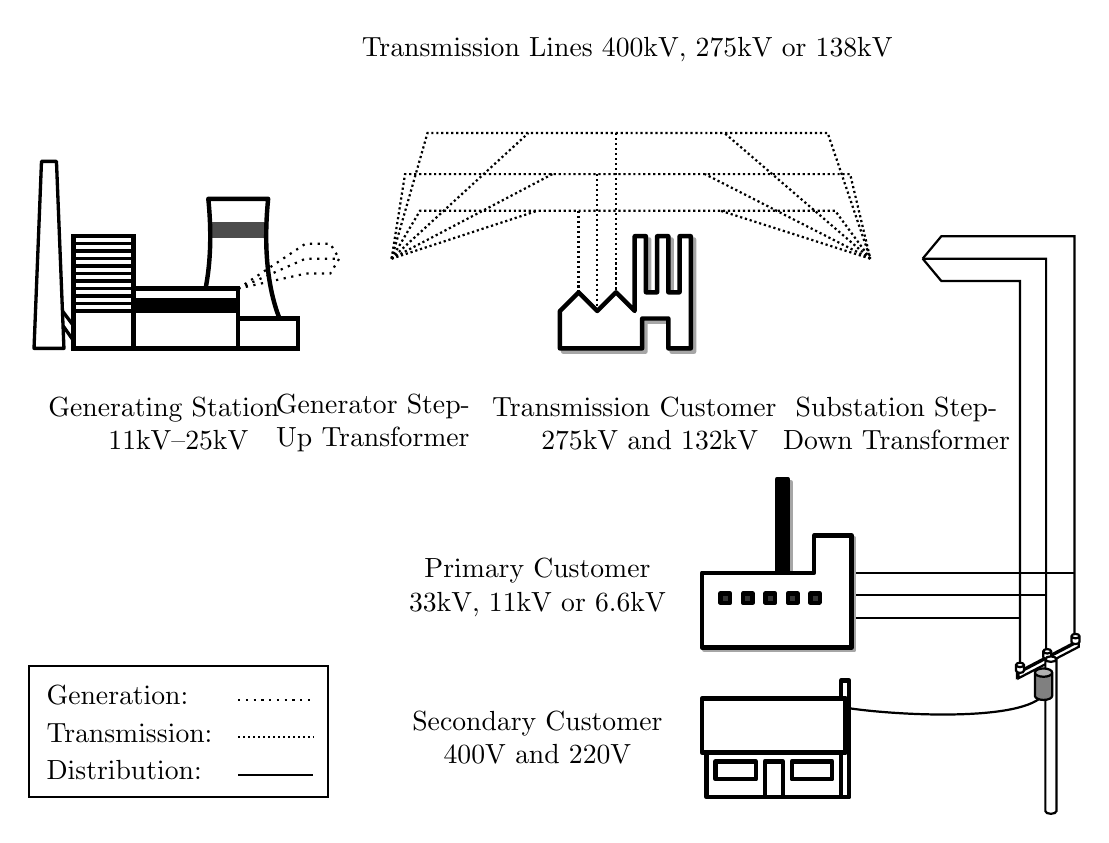
\begin{tikzpicture}[thick,scale=0.95]

  \tikzstyle{generation lines}=[thick,dotted]
  \tikzstyle{transmission lines}=[thick,densely dotted]
  \tikzstyle{distribution lines}=[thick]

  % Power Station.
  \begin{scope}[very thick]
    \draw[line join=round] (0.7mm,0) -- ++(1mm,25mm) -- ++(2mm,0) --
    ++(1mm,-25mm) -- cycle;

    \draw[ultra thick] (6mm,0) rectangle ++(8mm,15mm);
    \foreach \y in {0.5,0.6,...,1.5}
      \draw (6mm,\y) -- ++(8mm,0);

    \draw (6mm,1mm) -- ++(-1.4mm,2mm);
    \draw (6mm,3mm) -- ++(-1.5mm,2mm);

    \begin{scope}[ultra thick,xshift=2cm,yshift=0cm]
      \filldraw[fill=black!70,draw=black!70] (4.3mm,15mm) rectangle
      ++(7.4mm,1.6mm);

      \draw[line join=round] (0,0) .. controls (3mm,3mm) and
      (5mm,10mm) .. (4mm,20mm)-- (12mm,20mm) --
      (12mm,20mm) .. controls (11mm,10mm) and (13mm,3mm) .. (16mm,0mm);
%      \draw (4mm,20mm) -- (12mm,20mm);
    \end{scope}

    \filldraw[ultra thick,fill=white] (14mm,0) rectangle ++(14mm,8mm);
    \filldraw[fill=black] (14mm,5mm) rectangle ++(14mm,1.5mm);

    \filldraw[ultra thick,fill=white] (28mm,0) rectangle ++(8mm,4mm);

%     \begin{scope}[xshift=2cm,yshift=3cm]
%       \draw (0,0) to[out=30,in=270]
%             (3mm,15mm) to[out=0,in=180]
%             (9mm,15mm) to[out=-90,in=150]
%             (12mm,0);
%     \end{scope}
  \end{scope}

  \transformer{0cm}{4.2cm}
  \transformer{0cm}{11.3cm}

  \transmissiontower{60cm}{29.75mm}
  \transmissiontower{100cm}{29.75mm}

  \draw[generation lines] (2.8,0.8) -- (3.7,1.4) -- ++(0.33,0) -- (4.15,1.2);
  \draw[generation lines] (2.8,0.8) -- (3.7,1.2) -- (4.15,1.2);
  \draw[generation lines] (2.8,0.8) -- (3.7,1) -- ++(0.33,0) -- (4.15,1.2);

  \coordinate (trx12) at (4.85,1.2);
  \coordinate (trx21) at (11.25,1.2);
  \coordinate (trx22) at (11.95,1.2);
  \draw[transmission lines] (trx12) -- (5.33,2.88) -- ++(5.35,0) -- (trx21);
  \draw[transmission lines] (trx12) -- (5.03,2.33) -- ++(5.95,0) -- (trx21);
  \draw[transmission lines] (trx12) -- (5.23,1.84) -- ++(5.55,0) -- (trx21);
  % generator transformer
  \draw[transmission lines] (4.85,1.2) -- (6.68,2.88);
  \draw[transmission lines] (4.85,1.2) -- (7,2.33);
  \draw[transmission lines] (4.85,1.2) -- (6.8,1.84);
  % substation transformer
  \draw[transmission lines] (trx21) -- (9.3,2.88);
  \draw[transmission lines] (trx21) -- (9.04,2.33);
  \draw[transmission lines] (trx21) -- (9.25,1.84);
  % transmission customer
  \draw[transmission lines] (7.85,2.88) -- ++(0,-2.2);
  \draw[transmission lines] (7.6,2.33) -- ++(0,-1.85);
  \draw[transmission lines] (7.35,1.84) -- ++(0,-1.1);

  \draw[distribution lines] (13.25,-4.2) -- (13.25,0.9) -- (12.2,0.9) --
  (trx22);
  \draw[distribution lines] (13.6,-4.1) -- (13.6,1.2) -- (trx22);
  \draw[distribution lines] (13.98,-3.9) -- (13.98,1.5) -- (12.2,1.5) --
  (trx22);
  % primary customer
  \draw[distribution lines] (13.25,-3.6) -- (11.05,-3.6);
  \draw[distribution lines] (13.6,-3.3) -- (11.05,-3.3);
  \draw[distribution lines] (13.98,-3.0) -- (11.05,-3.0);
  % secondary customer
  \draw[distribution lines] (13.55,-4.65)  .. controls (13.2,-5.) and
  (11.5,-4.9) .. (10.9,-4.8);

  % Transmission customer.
  \begin{scope}[xshift=7.1cm,yshift=0cm,line join=round,ultra
  thick,xscale=0.5,yscale=0.5]
    \draw[draw=gray!70,xshift=2.5pt,yshift=-2.5pt]
    (0,0) -- (0,1) -- (0.5,1.5) -- (1,1) -- (1.5,1.5) -- (2,1) -- (2,3) --
    (2.3,3) -- (2.3,1.5) -- (2.6,1.5) -- (2.6,3) -- (2.9,3) -- (2.9,1.5) --
    (3.2,1.5) -- (3.2,3) -- (3.5,3) -- (3.5,0) -- (2.9,0) -- (2.9,0.8) --
    (2.2,0.8) -- (2.2,0) -- cycle;

    \filldraw[fill=white] (0,0) -- (0,1) -- (0.5,1.5) -- (1,1) -- (1.5,1.5) --
    (2,1) -- (2,3) -- (2.3,3) -- (2.3,1.5) -- (2.6,1.5) -- (2.6,3) -- (2.9,3) -- (2.9,1.5) --
    (3.2,1.5) -- (3.2,3) -- (3.5,3) -- (3.5,0) -- (2.9,0) -- (2.9,0.8) --
    (2.2,0.8) -- (2.2,0) -- cycle;
  \end{scope}

  % Distribution customer.
  \begin{scope}[xscale=0.5,yscale=0.5,xshift=18cm,yshift=-8cm,ultra thick,line
  join=round]
    \draw[draw=gray!70,xshift=2pt,yshift=-2pt] (2,2) rectangle ++(0.3,2.5);
	\filldraw[fill=black] (2,2) rectangle ++(0.3,2.5);

	\draw[draw=gray!70,xshift=2pt,yshift=-2pt] (0,0) -- (0,2) -- (3,2) -- (3,3) --
	(4,3) -- (4,0) -- cycle;
	\filldraw[fill=white] (0,0) -- (0,2) -- (3,2) -- (3,3) -- (4,3) -- (4,0) --
	cycle;

	\foreach \x in {0.5,1.1,1.7,2.3,2.9}
	  \filldraw[fill=black!80] (\x,1.2) rectangle ++(2.5mm,2.5mm);

  \end{scope}

  % House.
  \begin{scope}[xscale=0.6,yscale=0.6,xshift=15.1cm,yshift=-10cm,ultra
  thick,line join=round]
    \draw (0,0) rectangle ++(3,1);
    \draw (3,0) rectangle ++(0.18,2.6);
    \filldraw[fill=white] (-0.1,1) rectangle ++(3.2,1.2);

    \draw (0.2,0.4) rectangle ++(0.9,0.4);
    \draw (1.3,0) rectangle ++(0.4,0.8);
    \draw (1.9,0.4) rectangle ++(0.9,0.4);

    \coordinate (d1) at (0.45,1.3);
    \coordinate (d2) at (2.15,1.3);
    \dormer{d1};
    \dormer{d2};
  \end{scope}

  \node[text width=33mm,text centered] at (2,-1) {Generating Station
  \newline 11kV--25kV};
  \node[text width=2.5cm,text centered] at (4.6,-1) {Generator Step-Up
  Transformer};
  \node[text width=8cm,text centered] at (8,4) {Transmission Lines 400kV,
  275kV or 138kV};
  \node[text width=4cm,text centered] at (8.3,-1) {Transmission Customer
  \newline 275kV and 132kV};
  \node[text width=3cm,text centered] at (11.6,-1) {Substation Step-Down
  Transformer};
  \node[text width=4cm,text centered] at (6.8,-3.2) {Primary Customer 33kV,
  11kV or 6.6kV};
  \node[text width=4cm,text centered] at (6.8,-5.2) {Secondary Customer 400V
  and 220V};

  % Line key.
  \begin{scope}[yshift=-6cm]
    \draw (0,0) rectangle ++(4,1.75);
%    \node[above right] at (0.1,1.5) {\textbf{Line Key}};

    \node[above right] at (0.1,1.1) {Generation:};
    \draw[generation lines] (2.8,1.3) -- ++(1,0);

    \node[above right] at (0.1,0.6) {Transmission:};
    \draw[transmission lines] (2.8,0.8) -- ++(1,0);

    \node[above right] at (0.1,0.1) {Distribution:};
    \draw[distribution lines] (2.8,0.3) -- ++(1,0);
  \end{scope}

  % Pole.
  \begin{scope}[xscale=0.7,yscale=0.7,xshift=19.5cm,yshift=-5.8cm,thick]
    \draw (-0.63,-0.49) -- ++(1.15,0.6) -- ++(0,0.1) -- ++(-1.15,-0.6) -- cycle;
    \filldraw[fill=white] (-0.6,-0.5) -- ++(1.15,0.6) -- ++(0,0.1) --
    ++(-1.15,-0.6) -- cycle;

    \node[draw,cylinder,rotate=90,minimum width=1mm,minimum
    height=0.75mm,inner sep=0.8pt,cylinder uses custom fill,cylinder end
    fill=white, cylinder body fill=white] at (-0.57,-0.35) {};
    \node[draw,cylinder,rotate=90,minimum width=1mm,minimum
    height=0.75mm,inner sep=0.8pt,cylinder uses custom fill,cylinder end
    fill=white, cylinder body fill=white] at (0.49,0.2) {};
    \node[draw,cylinder,rotate=90,minimum width=1mm,minimum
    height=0.75mm,inner sep=0.8pt,cylinder uses custom fill,cylinder end
    fill=white, cylinder body fill=white] at (-0.5mm,-0.9mm) {};

    \node[draw,cylinder,rotate=90,aspect=0.5,minimum width=1mm,minimum
    height=2cm,inner sep=2pt,left,cylinder uses custom fill,cylinder end
    fill=white, cylinder body fill=white] at (0.2mm,-0.6mm) {};

%    \filldraw[fill=white] (0,-1) rectangle ++(-3mm,4mm);
    \node[draw,cylinder,rotate=90,aspect=0.75,minimum width=2.2mm,minimum
    height=4mm,inner sep=2pt,cylinder uses custom fill,cylinder end
    fill=black!30, cylinder body fill=black!50] at (-1.2mm,-7mm) {};
  \end{scope}

  \end{tikzpicture}
  \end{footnotesize}
  \caption{Basic structure of a three phase AC power system.}
  \label{fig:powersystem}
\end{figure}

Generation and bulk movement of electricity in the UK takes place in a
three-phase alternating current (AC) power system.  These phases are
high voltage, sinusoidal electrical waveforms, offset in time from each
other by 120 degrees and oscillating at a frequency of almost exactly 50Hz.
Synchronous generators (or alternators), typically rotating at 3600rpm or
1800rpm, generate apparent power $S$ at a line voltage $V_l$, typically
between 11kV and 25kV.  One of the principal reasons that alternating current,
and not direct current (DC), systems are common in electricity supply is that
they allow power to be transformed between voltages with very high efficiency.
The apparent power conducted by a three-phase transmission line $l$ is the
product of the line current $I_l$ and the line voltage
\begin{equation}
S = \sqrt{3} V_l I_l .
\end{equation}
For a constant quantity of transmitted power, increasing the line voltage has
an inverse effect on the line current.  Ohmic heating losses are proportional to the
square of line current
\begin{equation}
P_{r} = 3 I_l^2 R
\end{equation}
where $R$ is the resistance of the transmission line.  Hence reducing the line
current causes a large reduction in energy wasted through heating losses.  A
consequence of higher voltages is the larger extent and integrity of the
insulation required between conductors, neutral and earth.  This results in
the need for large transmission towers and in high cable costs when
undergrounding systems.

The UK transmission system operates at 400kV and 275kV (also 132kV in
Scotland), but systems with voltages upto and beyond 1000kV are used in
larger countries.  For transmission over very long distances or
undersea, high voltage DC (HVDC) systems have become econmically viable in
recent years.  The ability to
transform power between voltages and transmit large volumes over long
distances allows for generation to take place at high capacity power stations,
which offer economies of scale and lower operating costs. It allows electricity to
be transmitted across country borders and from renewable energy plant such as
hydro power stations located in remote areas.  A HVDC interconnector between
Folkstone in the UK and Sangatte in France allows upto 2GW of
electricity to be imported/exported.  The Moyle HVDC interconnector can export
upto 500MW from Auchencrosh in Scotland to Ballycronan More in Northern
Ireland or import upto 80MW.  Further HVDC interconnectors are planned between
England and the Netherlands and between Wales and The Republic of Ireland.
Figure \ref{fig:uk_gen} diagrams the exisitng interconnectors and illustrates
how the UK's larger power stations are located away from large load centres and
close to sources of fuel.

%\begin{figure}
\label{fig:uk_gen}
\centering
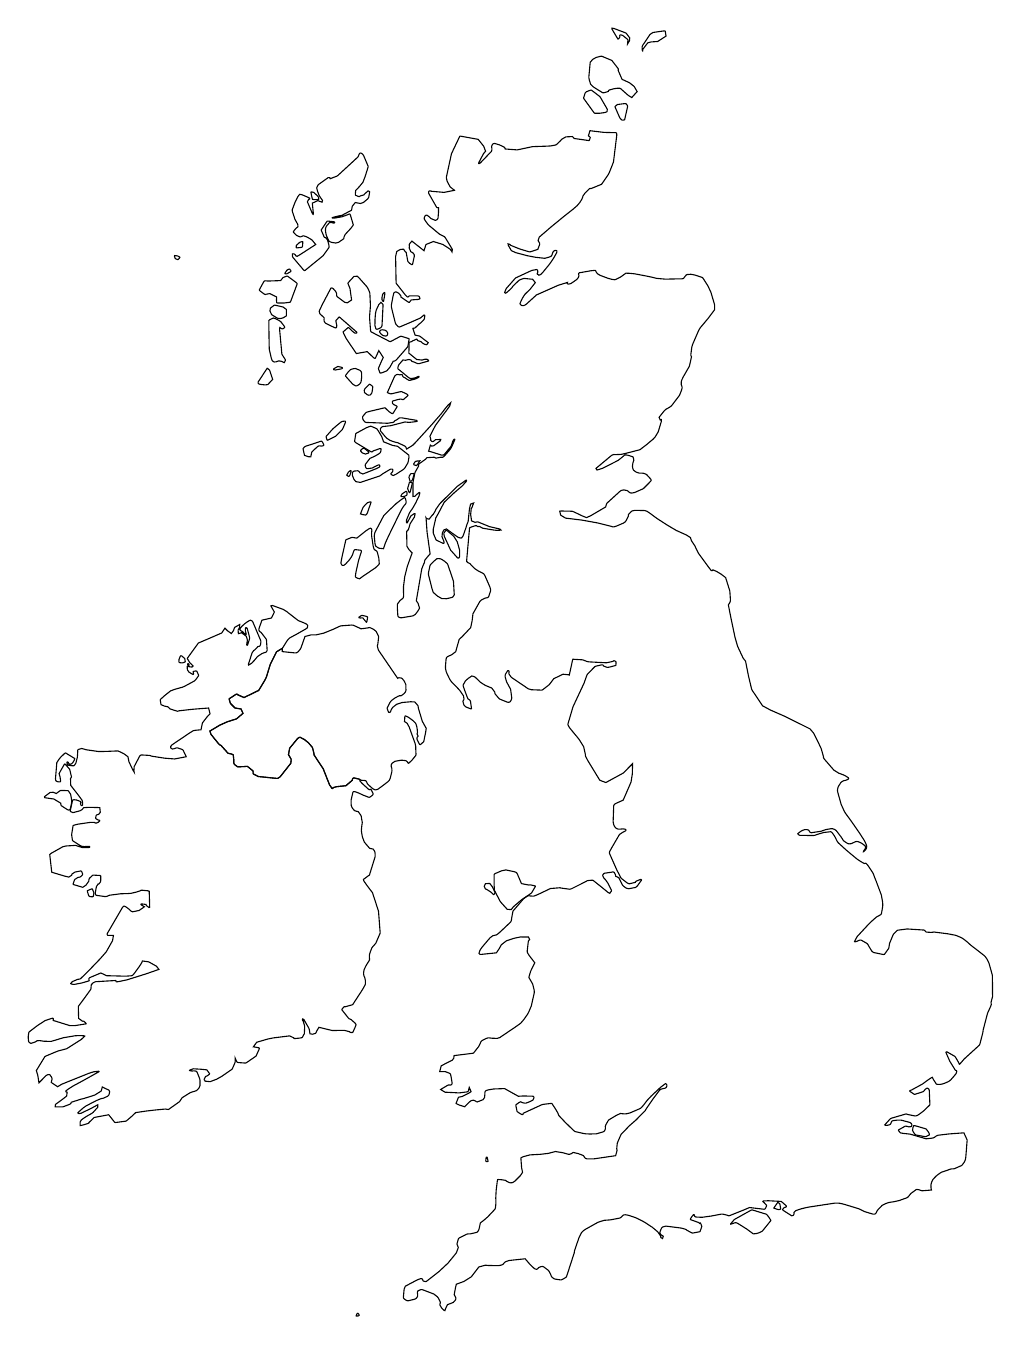
\begin{tikzpicture}[xscale=0.9,yscale=0.9]
%% UK
\draw[-] (-7.0029232622551705, 63.9837806219489309) -- (-7.0258060967827030, 63.9828204421218985) -- (-7.0323004758755712, 63.9833082879295887) -- (-7.0326088308650583, 63.9890557764767038) -- (-7.0220958181545639, 64.0125222257489099) -- (-7.0193128308847310, 64.0177854183140198) -- (-7.0146752608982936, 64.0206672099693463) -- (-7.0075619454365272, 64.0211414821389013) -- (-6.9992129836270438, 64.0134827506359159) -- (-6.9964311095521179, 64.0086940327863516) -- (-6.9908651350124549, 63.9986312143424527) -- (-6.9899367304591715, 63.9952760643323018) -- (-6.9979762240843524, 63.9866612283415321) -- (-7.0029232622551705, 63.9837806219489309);
\draw[-] (-1.1796771342243169, 65.3312023218514639) -- (-1.3005834595647072, 65.1814307246090436) -- (-1.3262481681670295, 65.1668460228547133) -- (-1.3528412813226902, 65.1556788253213028) -- (-1.3822173817481276, 65.1474224436747988) -- (-1.4276724694237668, 65.1411126953723141) -- (-1.5222940365980271, 65.2105816789109412) -- (-1.6397984382996860, 65.2844913944839647) -- (-1.6626801596323102, 65.2956884443617440) -- (-1.6688650705407289, 65.2981214176328706) -- (-1.6833978300638686, 65.2986013647504961) -- (-1.6957676518807836, 65.2961701287888872) -- (-1.7121561073153138, 65.2893549958920261) -- (-1.7467887140960758, 65.2786526525282511) -- (-1.7477160054543839, 65.2840097788230338) -- (-1.7263793986540594, 65.3098020983365046) -- (-1.6957676518807836, 65.3448401326821511) -- (-1.4570485698491926, 65.4778623406687785) -- (-1.4437525698688107, 65.4793211599138232) -- (-1.4375676589603255, 65.4783433443759293) -- (-1.2446142459836651, 65.4188713350837503) -- (-1.2399755628022537, 65.4149770690533217) -- (-1.2177116646436212, 65.3891533085663639) -- (-1.1796771342243169, 65.3312023218514639);
\draw[-] (-1.0445475175452477, 65.4890718676173833) -- (-1.0692860479841699, 65.4837012852078715) -- (-1.0828915161489963, 65.4866349593902157) -- (-1.1382417933611999, 65.5037018683566288) -- (-1.1373145020028919, 65.5100519498169547) -- (-1.1342220465486772, 65.5144337237093737) -- (-1.0862923265927509, 65.5817915926744632) -- (-1.0807263520530916, 65.5827583437858124) -- (-1.0736152629811373, 65.5808143068277332) -- (-1.0566078711777789, 65.5681159279046568) -- (-1.0535154157235662, 65.5627524449294867) -- (-1.0420739984597387, 65.4944305123412676) -- (-1.0445475175452477, 65.4890718676173833);
\draw[-] (-5.1782131309936190, 66.1624314043866235) -- (-5.1915080177790376, 66.1604734784666562) -- (-5.1976940418824871, 66.1624314043866235) -- (-5.2023316118689351, 66.1658764772080019) -- (-5.2035683714116256, 66.1727652906445485) -- (-5.2001675609678122, 66.2081763889622152) -- (-5.1980023968719067, 66.2219617782211429) -- (-5.1936731818749333, 66.2254093770570051) -- (-5.1862526246186658, 66.2254093770570051) -- (-5.1834685241539926, 66.2204754228513366) -- (-5.1723365750746755, 66.1712922287497634) -- (-5.1729555114434422, 66.1648903854284498) -- (-5.1782131309936190, 66.1624314043866235);
\draw[-] (1.0071319234947749, 66.5148046748936110) -- (1.0009481257811286, 66.5133129436408979) -- (0.9854869617049711, 66.5152936273477025) -- (0.8766409899971805, 66.5350462178021047) -- (0.8695287877301947, 66.5370274329331863) -- (0.8528308641112826, 66.5464184115659236) -- (0.8454091936599760, 66.5553070508684215) -- (0.8296396745943401, 66.5795231799295664) -- (0.8246915232284789, 66.5899085685546908) -- (0.8181982573305763, 66.6042485021037578) -- (0.8243831682391907, 66.6423220726047703) -- (0.8336594214068608, 66.6670541160774803) -- (0.8463375982133157, 66.6690367826504513) -- (0.8806607368097014, 66.6606254801249491) -- (0.9932169871455656, 66.6274875414197396) -- (1.0065141003207876, 66.6230311247177127) -- (1.0117706066761263, 66.6195683574217554) -- (1.0358890875513136, 66.5874384479331098) -- (1.0426929348285683, 66.5780427120904506) -- (1.0507324284538633, 66.5627182570993483) -- (1.0547521752663838, 66.5513580052493410) -- (1.0550616434507036, 66.5444369667400082) -- (1.0541332388973641, 66.5380180586695644) -- (1.0491862007265356, 66.5345589245572455) -- (1.0071319234947749, 66.5148046748936110);
\draw[-] (-5.0888469569797321, 69.9300095581513688) -- (-5.0956496910620874, 69.9289760259954107) -- (-5.1284277151261763, 69.9624789975047747) -- (-5.1924364223322428, 70.0037443621610151) -- (-5.2063513586814576, 70.0073568501536272) -- (-5.2131540927638129, 70.0171643343502978) -- (-5.2252144463963326, 70.0465773706661849) -- (-5.2230492823004377, 70.0517379973752270) -- (-5.2112995100471853, 70.0770368224225848) -- (-5.2082070545929806, 70.0827237147293403) -- (-5.2014043205106280, 70.0837592602865698) -- (-5.1503821451003597, 70.0868511045808873) -- (-5.1448161705606967, 70.0837592602865698) -- (-5.1104930319643840, 70.0388361337554528) -- (-5.0767877165421078, 69.9666131037944723) -- (-5.0755509569992947, 69.9593901611832649) -- (-5.0755509569992947, 69.9521678786899201) -- (-5.0770971847264903, 69.9444377422045704) -- (-5.0801896401806390, 69.9387737860242709) -- (-5.0888469569797321, 69.9300095581513688);
\draw[-] (-4.6234702597438675, 69.9057909760740870) -- (-4.6955184605751130, 69.8589054918475370) -- (-4.8151869131779046, 69.7564987295826455) -- (-4.8439440772344966, 69.7184525718326285) -- (-4.9005322271843044, 69.7210230822816186) -- (-4.9858764279958532, 69.8151549613515527) -- (-5.0031932879837226, 69.8388231323254445) -- (-5.0845177419827694, 69.9944640898785053) -- (-5.0863734378942835, 70.2077994553168736) -- (-5.0838999188088447, 70.2140078896493947) -- (-5.0761687801732736, 70.2238261832096384) -- (-4.9812388580094167, 70.2647178425278724) -- (-4.9305261507836553, 70.2755786533527385) -- (-4.9237234167013000, 70.2766167329784679) -- (-4.9159933912606499, 70.2766167329784679) -- (-4.8022003813819047, 70.2522934781159165) -- (-4.7783891423012905, 70.2440066879090921) -- (-4.7684939527645982, 70.2362460637690731) -- (-4.7610733955083289, 70.2269384201685085) -- (-4.7533422568727595, 70.2088366432553386) -- (-4.7001560305615593, 70.0842705310542726) -- (-4.5940941593184412, 70.0636215436610286) -- (-4.5888376529631616, 70.0662014424396062) -- (-4.5817254506964353, 70.0672219011699724) -- (-4.5752321847984625, 70.0667125995359612) -- (-4.5195713262068518, 70.0543193664251760) -- (-4.5047290984993955, 70.0501918181619772) -- (-4.5044207435099093, 70.0434871027729713) -- (-4.5529671734448556, 69.9604240911487238) -- (-4.5656453502512573, 69.9470137517094201) -- (-4.6234702597438675, 69.9057909760740870);
\draw[-] (-7.0724979440010349, 73.7302121538367743) -- (-6.9630341491192604, 73.6798873069975571) -- (-6.8665579992283856, 73.6928699654771862) -- (-6.8455308606123761, 73.6977419466528261) -- (-6.8374902537923701, 73.6961237605069641) -- (-6.7948181533866157, 73.6766497707508705) -- (-6.7889438238574771, 73.6734123703486290) -- (-6.7533839257184081, 73.6458367050812370) -- (-6.7468895466255940, 73.6344788169192555) -- (-6.7209142566439137, 73.5820658320416499) -- (-6.7165850416468853, 73.5691173504016973) -- (-6.7162766866574666, 73.5610188485555767) -- (-6.7264802311835776, 73.4676597268901617) -- (-6.7342113698191373, 73.4374616953618613) -- (-6.7193691421116259, 73.3803434692123631) -- (-6.5060064136928819, 73.0674569230986890) -- (-6.4469447446576362, 72.9811214649410687) -- (-6.4364317319471525, 72.9880847309429726) -- (-6.4293195296802930, 72.9891594719649248) -- (-6.3974699101694723, 72.9854046966363086) -- (-6.3857190247212676, 72.9789722207710412) -- (-6.3807719865504389, 72.9752198682372040) -- (-6.3569618606647316, 72.9457591220409540) -- (-6.3541788733948996, 72.9404020727488813) -- (-6.3371725947863213, 72.9055883468396502) -- (-6.3319149752361987, 72.8938105887541354) -- (-6.3302140134169340, 72.8266319852239548) -- (-6.3300592793246766, 72.8146294135640630) -- (-6.3312960388673671, 72.8071388556083718) -- (-6.3346979625060316, 72.7975067262687787) -- (-6.3377904179602469, 72.7894885635974447) -- (-6.3411912284040595, 72.7836150058597013) -- (-6.3575807970335525, 72.7649118803198149) -- (-6.3925840977184913, 72.7385100494529411) -- (-6.3959236824423993, 72.7365886930866026) -- (-6.4001905585244288, 72.7359424818155986) -- (-6.4198573729628965, 72.7359424818155986) -- (-6.4407598337492056, 72.7275056873325099) -- (-6.4747746173559886, 72.7098715758086769) -- (-6.4806500600800341, 72.7066743680499741) -- (-6.5261051477556737, 72.6741041908976655) -- (-6.5356919823027564, 72.6655569033496533) -- (-6.5434220077434206, 72.6559557783055823) -- (-6.5548634250071203, 72.6410213468755188) -- (-6.5582642354509328, 72.6346173652211888) -- (-6.5944430699586567, 72.5626252458072258) -- (-6.5956798295014698, 72.5546178732590903) -- (-6.5771273231658185, 72.5066753328296016) -- (-6.5731075763532960, 72.5018777198215076) -- (-6.5659953740864365, 72.4997417076361756) -- (-6.5536255522695210, 72.5040137907153053) -- (-6.5489879822830730, 72.5082707677635767) -- (-6.5455860586444192, 72.5141216153487704) -- (-6.5397106159203719, 72.5354422948133788) -- (-6.5186845904994062, 72.5695510510068971) -- (-6.4747746173559886, 72.6042008622737285) -- (-6.4599323896485439, 72.6154085883551943) -- (-6.3904200468174919, 72.6380305794546075) -- (-6.3876359463527628, 72.6393136948495766) -- (-6.3831842799159171, 72.6399514187717585) -- (-6.2663611534978916, 72.6500923171150248) -- (-6.2329641930649791, 72.6495505648691449) -- (-6.2082267758209522, 72.6474258567264997) -- (-6.2023513330968507, 72.6442158518950123) -- (-6.1658630304045650, 72.6020773945240876) -- (-6.1618432835920425, 72.5972719671244135) -- (-6.1596792326910430, 72.5908715918637881) -- (-6.1534954349774544, 72.5551589637357353) -- (-6.0996902722974893, 72.3757465641085957) -- (-6.0505237927987459, 72.2859314726269417) -- (-6.0452672864435879, 72.2816866482608305) -- (-6.0443399950852790, 72.2747711397402384) -- (-6.0505237927987459, 72.2307037489979535) -- (-6.0517605523415599, 72.2227457613507227) -- (-6.0792820700503132, 72.0875327480730732) -- (-6.1235627370980730, 72.0476009365361563) -- (-6.1269023218219161, 72.0460072920672303) -- (-6.1315398918083623, 72.0456946670712313) -- (-6.1382190612559269, 72.0498256119554554) -- (-6.1423011469833275, 72.0561740066328724) -- (-6.1729140069515118, 72.1178432526730830) -- (-6.1742131054089571, 72.1216574618557331) -- (-6.1747697028630339, 72.1257981604609597) -- (-6.1751403967672642, 72.1353340532135690) -- (-6.1734706044054670, 72.1436133074174109) -- (-6.1719856023982960, 72.1477418120683609) -- (-6.1703169232312813, 72.1512368014109740) -- (-6.1584424731483516, 72.1662015573961639) -- (-6.1735941690402463, 72.1946327776669108) -- (-6.1689554858589020, 72.2084177023827039) -- (-6.1677187263160773, 72.2158507702469024) -- (-6.1711206499547426, 72.2620391868148317) -- (-6.1782317390266934, 72.3045196465163684) -- (-6.1803969031226016, 72.3108964894909292) -- (-6.1890553331164693, 72.3364090888652669) -- (-6.1912193840175345, 72.3422489316950390) -- (-6.1983315862842732, 72.3528773459226926) -- (-6.2335831294338000, 72.3863795566852986) -- (-6.2778014575666923, 72.4193694634128775) -- (-6.2997558875409965, 72.4331942638630011) -- (-6.3235660134267171, 72.4459695915053743) -- (-6.3371725947863213, 72.4502253069638300) -- (-6.3436647474895080, 72.4481041265556058) -- (-6.3458299115854162, 72.4411757237025284) -- (-6.3504674815718518, 72.3704286986644689) -- (-6.3183095070715014, 72.3502191493704458) -- (-6.3133624689006052, 72.3475629572975691) -- (-6.2840086323732827, 72.2921174758321854) -- (-6.2042114817879277, 72.0712883172326997) -- (-6.1984607168936368, 72.0519054644885131) -- (-6.1906683525381077, 72.0096577900071679) -- (-6.1925229352547237, 72.0061615234343009) -- (-6.1884363967477034, 71.9070889747031430) -- (-6.1918372071913934, 71.8922823172074317) -- (-6.2190492567157643, 71.8579459492132315) -- (-6.2431688507859864, 71.8288920508400395) -- (-6.2873871789188698, 71.7861341803120894) -- (-6.2932626216429703, 71.7829727875736410) -- (-6.2991369511721098, 71.7845534679413078) -- (-6.3031578111795410, 71.7892938010795945) -- (-6.3084143175348766, 71.8009055083681744) -- (-6.3278952284236780, 71.8162175129677962) -- (-6.3340801393321078, 71.8193916566658430) -- (-6.3418101647728928, 71.8209730746332156) -- (-6.3792257588232975, 71.8246720451384562) -- (-6.3965426188111651, 71.8257308269297283) -- (-6.4815773514383430, 71.8109395968941158) -- (-6.4871433259780051, 71.8082998224468838) -- (-6.5183751223148896, 71.7877130247355097) -- (-6.5276524886776572, 71.7798001242809960) -- (-6.5378560332037576, 71.7597564320121677) -- (-6.5387833245620648, 71.7439200073418561) -- (-6.5366192736610653, 71.7296815514854273) -- (-6.5298165395787233, 71.7112299139116800) -- (-6.5288892482204144, 71.7038447854441898) -- (-6.5276524886776572, 71.6801301669785715) -- (-6.5291976032098891, 71.6632665591996982) -- (-6.5511520331840716, 71.5758443567992515) -- (-6.5638302099905959, 71.5437453400720358) -- (-6.5718697036156968, 71.5337455058998444) -- (-6.5904244363410411, 71.5179699585191031) -- (-6.6439190176418492, 71.4764358974764349) -- (-6.7280264589105858, 71.4149532828921707) -- (-6.7546206852611528, 71.4081160387483038) -- (-6.7626601788862013, 71.4075960847200264) -- (-6.7703890911320759, 71.4091691925818708) -- (-6.7997663047523549, 71.4244046387076139) -- (-6.8693409864982069, 71.4869469920574829) -- (-6.8764520755700351, 71.4974594992190191) -- (-6.8860389101171187, 71.5211187542864053) -- (-6.8931511123839799, 71.5321698910731953) -- (-6.8980981505547438, 71.5358552129627441) -- (-6.9049008846372200, 71.5384839042752958) -- (-6.9763646581417023, 71.5444821208588735) -- (-6.9769501986632401, 71.5484843444543088) -- (-6.9825150600079962, 71.5542654852893634) -- (-6.9893177940904714, 71.5584709087092108) -- (-7.0004497431697894, 71.5611003604397524) -- (-7.0564189567507638, 71.5742697881845231) -- (-7.0684793103832959, 71.5742697881845231) -- (-7.0743536399125579, 71.5716379988097628) -- (-7.0799207276471190, 71.5668975909155165) -- (-7.0839393612647328, 71.5611003604397524) -- (-7.0857950571762576, 71.5553206085579632) -- (-7.0867234617294717, 71.5495242363596020) -- (-7.0864139935450234, 71.5437453400720358) -- (-7.1773241688963028, 71.4659110778357132) -- (-7.3109075578481750, 71.4517212755582847) -- (-7.3535807714488906, 71.4396411600454684) -- (-7.3560542905342743, 71.4354421204430992) -- (-7.3693514037096186, 71.4259761932989647) -- (-7.3749162650543738, 71.4296565156330843) -- (-7.3832663400587659, 71.4412149122176885) -- (-7.4089310486610884, 71.4790625924865424) -- (-7.4970593499373903, 71.7033228611207534) -- (-7.6272408152507865, 71.9007431920575613) -- (-7.6260040557080275, 71.9091935671282698) -- (-7.6476501306927345, 71.9985731638512618) -- (-7.6544528647750907, 72.0107552880336925) -- (-7.7002174206351119, 72.0647499265752458) -- (-7.7110399015301114, 72.0753557818916022) -- (-7.7639166596569291, 72.1182725565363683) -- (-7.8205036964118291, 72.1474211436751460) -- (-7.8266886073203805, 72.1490073198631734) -- (-7.8328724050338359, 72.1479594092299834) -- (-7.8573003540935344, 72.1341699132984928) -- (-7.9714028321566603, 71.9943439693719114) -- (-7.9877924007862227, 71.9039093591162839) -- (-7.9537776171793064, 71.8463257538275570) -- (-7.9509957431043832, 71.8405096505689897) -- (-7.9497578703667955, 71.8341711810092391) -- (-7.9547060217325241, 71.7824370353836230) -- (-8.1049873343034999, 71.5921527652666043) -- (-8.1117900683858526, 71.5863707173507180) -- (-8.1411661688113437, 71.5684720110599670) -- (-8.1600281433313810, 71.5695273260646161) -- (-8.4151356807975013, 71.5958409156538522) -- (-8.4714143625630385, 71.6253296331827300) -- (-8.4825463116423538, 71.6321877905362498) -- (-8.4865649452599676, 71.6374536407771529) -- (-8.4871838816288001, 71.6500840255570637) -- (-8.4859471220860438, 71.6643231549286952) -- (-8.4874933498131853, 71.6706345727760947) -- (-8.4912036284413244, 71.6769597813185442) -- (-8.5681999806382976, 71.7391824278839465) -- (-8.5743837783518853, 71.7391824278839465) -- (-8.6247870173932526, 71.7349539774515819) -- (-8.7002371418630950, 71.7328521791006466) -- (-8.7058031164027501, 71.7328521791006466) -- (-8.7401262549990726, 71.7576406714824628) -- (-8.7518771404471547, 71.7687120138182735) -- (-8.7580609381607424, 71.7803206601960682) -- (-8.7599166340722672, 71.7935270953576747) -- (-8.7602261022566488, 71.8352300916679809) -- (-8.7661004317859099, 71.8912226320808543) -- (-8.7670288363391258, 71.8975657377167607) -- (-8.7698118236089471, 71.9039093591162839) -- (-8.7945492408529731, 71.9134333705635953) -- (-8.8403137967129961, 71.9234648105225745) -- (-8.9392656920791929, 72.0335089879938550) -- (-8.9559636156981615, 72.0414495724894550) -- (-8.9677133879513455, 72.0509884924155841) -- (-8.9785358688463468, 72.0631635581097356) -- (-9.0799612832978571, 72.1887887214968629) -- (-9.0830526255571655, 72.1951560903659697) -- (-9.0966569805270208, 72.2370688139292838) -- (-8.9578193116096205, 72.3199290132569104) -- (-8.8508279226183877, 72.3677718164255168) -- (-8.7203358759258887, 72.4092567141278209) -- (-8.6297351687590496, 72.4869709600998249) -- (-8.6578733964468313, 72.5492896764626494) -- (-8.7379622040980731, 72.5610152620585325) -- (-8.7444554699960442, 72.5642218299825430) -- (-8.8013519749353168, 72.6212828739032119) -- (-8.8097009367448109, 72.6340738002136135) -- (-8.8248537458316161, 72.6874477576348141) -- (-8.8223802267462332, 72.6938560986459379) -- (-8.7308500018312802, 72.7542115639699034) -- (-8.7160066609288585, 72.7579551601936885) -- (-8.7101323313997767, 72.7558274826312470) -- (-8.7042568886756762, 72.7494140227861550) -- (-8.6152012960410111, 72.7098715758086769) -- (-8.4083329467151451, 72.8103421308553180) -- (-8.3298582716804948, 72.9397406628976483) -- (-8.3022699622771867, 72.9934431480368460) -- (-8.2865004432113576, 73.0411719854131150) -- (-8.2447545209689483, 73.1780552643971305) -- (-8.1556989283343526, 73.3560981568168415) -- (-8.0734538621464296, 73.4052055254939120) -- (-8.0762290570519308, 73.3604021916643774) -- (-8.0719009552499319, 73.3577092336918213) -- (-7.8981178717827270, 73.3399485301507497) -- (-7.8743077458970188, 73.3415592705125334) -- (-7.8637947331864035, 73.3469422167251253) -- (-7.8538995436498444, 73.3544851748558528) -- (-7.8452422268508739, 73.3636420084030050) -- (-7.8248329114087358, 73.3884230512439757) -- (-7.8143198986982414, 73.4045828096504067) -- (-7.7858710896311782, 73.4822204164690618) -- (-7.7555676978474439, 73.5712675034377099) -- (-7.6696045606670520, 73.5939488497813556) -- (-7.5972457784564593, 73.5944991958542687) -- (-7.4921111985717168, 73.6182708900636271) -- (-7.3619297332584415, 73.6707084761627584) -- (-7.2530837615505854, 73.7210117505796063) -- (-7.0981648789931722, 73.7329161862808036) -- (-7.0724979440010349, 73.7302121538367743);
\draw[-] (-6.8715050373992055, 73.8379695210110185) -- (-6.8807812905670085, 73.7832600602456523) -- (-6.8848021505744290, 73.7762111475643678) -- (-6.8888218973869506, 73.7729695658108824) -- (-6.9401524277866375, 73.8347097355013062) -- (-6.9716925791131965, 73.8325522273712949) -- (-6.9883916159270738, 73.8336387768109006) -- (-6.9936470090873781, 73.8363464388214368) -- (-6.9924102495446885, 73.8444738975947672) -- (-6.9716925791131965, 73.8591058736825801) -- (-6.9602522750443372, 73.8666990499032323) -- (-6.9451005791524985, 73.8683227714137871) -- (-6.8919143528411642, 73.8563974120414315) -- (-6.8776899483076344, 73.8509788231123423) -- (-6.8736702014951128, 73.8466317394497622) -- (-6.8715050373992055, 73.8379695210110185);
\draw[-] (-5.6813148904644057, 74.1224448039558865) -- (-5.7573828381081613, 74.1045051935063412) -- (-5.8148982794162780, 74.1055818828855166) -- (-5.8238661775945939, 74.1061339367365690) -- (-5.8297405071237227, 74.1093895688870532) -- (-5.8813805057079147, 74.1387610877897743) -- (-5.8918935184184091, 74.1469342381647181) -- (-5.9447713897400662, 74.1937355339982787) -- (-5.9469354406411314, 74.1980885397213257) -- (-5.9636333642600468, 74.2509224264682217) -- (-6.0115619710211901, 74.4402062352270093) -- (-6.0121809073898991, 74.4565901109882873) -- (-6.0115619710211901, 74.4740711477487309) -- (-6.0072327560242273, 74.4959241063293405) -- (-5.9902253642208096, 74.5741306596869578) -- (-5.9868245537770530, 74.5801401530546002) -- (-5.9787839469570994, 74.5905411749573517) -- (-5.9333299724763666, 74.6354196239535099) -- (-5.9283818211106398, 74.6398095599809608) -- (-5.8946776188831365, 74.6688284865043670) -- (-5.8615901266346091, 74.6699249460014158) -- (-5.8464384307427695, 74.6677438747256588) -- (-5.8322140262092379, 74.6628100707128368) -- (-5.8201536725766401, 74.6562361024135583) -- (-5.7867589385335307, 74.6343354844502755) -- (-5.7722250658156176, 74.6217349649787991) -- (-5.7530536231111338, 74.6047759187345179) -- (-5.7443951931172670, 74.5949147529115777) -- (-5.7382113954036775, 74.5834316876255485) -- (-5.6609066882172856, 74.3539575057537547) -- (-5.6593593472951813, 74.3468698871487703) -- (-5.6491546895741722, 74.1708769880291214) -- (-5.6488463345846975, 74.1627012938232753) -- (-5.6503925623118381, 74.1550925857417980) -- (-5.6537933727555281, 74.1491005721521361) -- (-5.6698734732007061, 74.1284367001547935) -- (-5.6813148904644057, 74.1224448039558865);
\draw[-] (-5.5842186910097880, 74.6792395677309884) -- (-5.5916403614609766, 74.6781410027926000) -- (-5.5996798550860767, 74.6797957592112738) -- (-5.6046268932569072, 74.6836182055192950) -- (-5.6983222822678226, 74.7883519927787290) -- (-5.7017230927114468, 74.7943782960279009) -- (-5.7870672935231404, 74.9800569936915053) -- (-5.7892324576189802, 74.9866588012657900) -- (-5.7951067871481188, 75.0152626494628691) -- (-5.7960351917013249, 75.0229709983748876) -- (-5.7957257235170072, 75.0301213791431962) -- (-5.7682053190030951, 75.0670151985259935) -- (-5.7629488126478261, 75.0708708918512997) -- (-5.7558366103809666, 75.0686625172509565) -- (-5.7447046613016495, 75.0615105170241748) -- (-5.6553396004826588, 74.9855558201984707) -- (-5.6064825891684311, 74.9080463499832234) -- (-5.5758697292002370, 74.7998657846959105) -- (-5.5721594505721086, 74.7861517497251640) -- (-5.5718510955826215, 74.7696973561821210) -- (-5.5737056782992385, 74.6962308683747551) -- (-5.5761791973846204, 74.6891115798903087) -- (-5.5842186910097880, 74.6792395677309884);
\draw[-] (-6.8146085324598671, 74.9894074120952183) -- (-6.7938908620283085, 74.8553019687044952) -- (-6.7926541024855505, 74.8476243138152029) -- (-6.7877070643147199, 74.8267558128109727) -- (-6.7830683811333765, 74.8135802982891533) -- (-6.7775024065936558, 74.8015073668317285) -- (-6.7632780020601242, 74.7888931753447963) -- (-6.7453433188984535, 74.7784671952330626) -- (-6.7373027120785105, 74.7685994690670412) -- (-6.7348291929930602, 74.7625574220919731) -- (-6.7128747630187462, 74.6765020599347764) -- (-6.7066909653052234, 74.5982069212986545) -- (-6.7097823075645326, 74.5921802524453028) -- (-6.7218426611971305, 74.5768645170390556) -- (-6.7645147616028156, 74.5374732900253179) -- (-6.9339675168781403, 74.4238120934865179) -- (-6.9846802241040251, 74.3856093732402570) -- (-7.0137468563450778, 74.3937930887875751) -- (-7.0323004758755712, 74.4030742609821374) -- (-7.0415767290433751, 74.4128950917924357) -- (-7.0437407799443728, 74.4183533986949897) -- (-7.0375569822307851, 74.4691497783805261) -- (-7.0363202226880945, 74.4762624584561337) -- (-6.9973572877155190, 74.6502186745265561) -- (-6.9608700982181961, 74.7614734581643603) -- (-6.9587060473171967, 74.7685994690670412) -- (-6.9590155155015792, 74.7768241316668281) -- (-6.9624163259453375, 74.7834084471687390) -- (-6.9676728323005408, 74.7872518633570280) -- (-6.9744755663830169, 74.7894363368714750) -- (-7.0412672608589242, 74.7965787752546731) -- (-7.0483794631257188, 74.7965787752546731) -- (-7.0551821972080724, 74.7943782960279009) -- (-7.0638406272019409, 74.7839515698293553) -- (-7.0669319694613817, 74.7768241316668281) -- (-7.0715717658376329, 74.7636571971505361) -- (-7.0758998676395652, 74.7504925238251161) -- (-7.0805385508209762, 74.7351471215254577) -- (-7.0882685762616378, 74.7165054253556633) -- (-7.1018751576213681, 74.6912932589130634) -- (-7.1167173853288226, 74.6699249460014158) -- (-7.1365066512071111, 74.6436457851954600) -- (-7.1794893329922100, 74.5971095161421260) -- (-7.1940232057101241, 74.5845151081038296) -- (-7.2060813329529623, 74.5768645170390556) -- (-7.2190700911386427, 74.5741306596869578) -- (-7.2261811802106068, 74.5757674170504004) -- (-7.2373142424848211, 74.5834316876255485) -- (-7.2413328761024456, 74.5899994202646752) -- (-7.2459715592837908, 74.6009416365464517) -- (-7.2468988506420979, 74.6173598580372186) -- (-7.2357669015627160, 74.6781410027926000) -- (-7.2305103952074443, 74.7022499345640227) -- (-7.1797976879816838, 74.9294811654025210) -- (-7.1708320161932395, 74.9393696349386431) -- (-7.0907420953470890, 74.9707057372927324) -- (-7.0239515140660878, 74.9591662416753763) -- (-6.8931511123839799, 75.0637028274236684) -- (-6.8606825565042158, 75.0857404231464898) -- (-6.8371818988028821, 75.0978582540880382) -- (-6.8313064560788455, 75.0995082201339557) -- (-6.8232669624537348, 75.0978582540880382) -- (-6.8149180006441954, 75.0884925946366053) -- (-6.8112066088211458, 75.0741677132789391) -- (-6.8158452920025017, 75.0213246628295849) -- (-6.8146085324598671, 74.9894074120952183);
\draw[-] (-6.8950068082955038, 75.2875816067446237) -- (-6.9018095423778592, 75.2853808811344294) -- (-6.9469551618691145, 75.2931165030230574) -- (-6.9720020472975124, 75.3013997151634698) -- (-6.9398429596023110, 75.3831804928181270) -- (-6.9336591618886656, 75.3942366762459102) -- (-6.9135593146311018, 75.4202451230086979) -- (-6.9045914164527824, 75.4296495299580840) -- (-6.8779994164920844, 75.4545443353571272) -- (-6.8724334419524205, 75.4589695557984754) -- (-6.8337799751642274, 75.4717086888353208) -- (-6.8248131901808744, 75.4700367183474867) -- (-6.8235764306381830, 75.4628450720732218) -- (-6.8773804801232510, 75.3074685431678006) -- (-6.8903681251141480, 75.2909017011591857) -- (-6.8950068082955038, 75.2875816067446237);
\draw[-] (-6.6201088917560096, 74.8926535461730367) -- (-6.6479387644543717, 74.8102946762800798) -- (-6.7094739525750544, 74.8168818679460941) -- (-6.7153482821042623, 74.8196263689391401) -- (-6.7382311166316597, 74.8339037066244828) -- (-6.7493630657109760, 74.8410344790385267) -- (-6.7577120275204621, 74.8498124856747467) -- (-6.7611128379642835, 74.8564030754953649) -- (-6.7632780020601242, 74.8640954496411837) -- (-6.7672977488726485, 74.8860598371952335) -- (-6.7771929384093275, 74.9866588012657900) -- (-6.7768834702249441, 74.9949069102666215) -- (-6.7731731915968156, 75.0196763816080647) -- (-6.7669882806882633, 75.0422304051383549) -- (-6.6436095494573326, 75.2765388573250362) -- (-6.6300029680977275, 75.2903410523402812) -- (-6.5749621590699130, 75.3455887014666672) -- (-6.5697067659095385, 75.3505667103738404) -- (-6.4667351237308308, 75.4479020050150382) -- (-6.4064366951528937, 75.4949586523851366) -- (-6.3953058592684755, 75.5032637848129724) -- (-6.3578902652179359, 75.5287450086855188) -- (-6.3513958861250677, 75.5298558557390294) -- (-6.3390271775029374, 75.5226446126277864) -- (-6.3285130515975467, 75.4800112920444803) -- (-6.3278952284236780, 75.4722567205029122) -- (-6.3278952284236780, 75.4633930401195556) -- (-6.3297498111402932, 75.4545443353571272) -- (-6.3350074306904149, 75.4418240020565349) -- (-6.3479939624863482, 75.4263234002121976) -- (-6.3541788733948996, 75.4207907939216824) -- (-6.3640740629314587, 75.4075125810060740) -- (-6.3789162906389141, 75.3848366286851501) -- (-6.3965426188111651, 75.3560922423725543) -- (-6.4030358847091371, 75.3428252705841146) -- (-6.5075526414200793, 75.1292593258437336) -- (-6.5724886399844635, 74.9965705021248681) -- (-6.6201088917560096, 74.8926535461730367);
\draw[-] (-6.3841739101891593, 75.5442524602054419) -- (-6.3925217588037464, 75.5442524602054419) -- (-6.3987066697122312, 75.5475837323260038) -- (-6.4008707206132307, 75.5536721574928549) -- (-6.3943774547152596, 75.5664291030577004) -- (-6.3847917333629614, 75.5836026732639539) -- (-6.3356252538643396, 75.6168792342150624) -- (-6.3291319879663686, 75.6190875388017361) -- (-6.3226387220684082, 75.6174263127579849) -- (-6.3176916838975776, 75.6118818333803375) -- (-6.3161443429755284, 75.6063377569595900) -- (-6.3158359879860528, 75.5980233957838266) -- (-6.3158359879860528, 75.5741772850843887) -- (-6.3183095070715014, 75.5669758199501160) -- (-6.3288225197819852, 75.5592124081484258) -- (-6.3479939624863482, 75.5509031804494953) -- (-6.3600543161189362, 75.5470211959309665) -- (-6.3841739101891593, 75.5442524602054419);
\draw[-] (-6.2672873316613016, 75.6218609883801776) -- (-6.2762552298396201, 75.6013430428464090) -- (-6.2830579639219630, 75.6035668679760420) -- (-6.2873871789188698, 75.6074497342233087) -- (-6.3043945707223541, 75.6529289173210202) -- (-6.3065586216233527, 75.6595891190419252) -- (-6.2830579639219630, 75.7400929078758054) -- (-6.2805844448365145, 75.7484387748825583) -- (-6.2444056103286778, 75.7428847616749437) -- (-6.2410036866900800, 75.7367652157195437) -- (-6.2415536049745990, 75.7278867479797952) -- (-6.2672873316613016, 75.6218609883801776);
\draw[-] (-6.2524451039537787, 75.7656533866854858) -- (-6.2592478380361225, 75.7623265789117966) -- (-6.2682157362145077, 75.7639889644045610) -- (-6.2734722425697873, 75.7678820090119700) -- (-6.2873871789188698, 75.8140215277136917) -- (-6.2846041916490361, 75.8301497315207769) -- (-6.2821295593687472, 75.8368254364714147) -- (-6.2682157362145077, 75.8601890024386023) -- (-6.2583205466778260, 75.8696478168019866) -- (-6.2499715848683302, 75.8701987157562030) -- (-6.2224511803544837, 75.8707636417308038) -- (-6.2159568012615489, 75.8674162159784942) -- (-6.2156473330772322, 75.8590733323983386) -- (-6.2175041421836532, 75.8507293596652090) -- (-6.2372934080619400, 75.7862156007997498) -- (-6.2434783189703698, 75.7745522609161526) -- (-6.2524451039537787, 75.7656533866854858);
\draw[-] (-7.1297050303196636, 75.8351454424441158) -- (-7.1355804730437091, 75.8318155995208230) -- (-7.1448567262115583, 75.8323662249581787) -- (-7.1612451816461560, 75.8446031502101050) -- (-7.1649554602742951, 75.8490650807681135) -- (-7.1426915621155276, 75.8907891677579869) -- (-7.1176446766871306, 75.9102827979246086) -- (-7.1108419426047780, 75.9124996200001192) -- (-7.1043486767066941, 75.9097175787501897) -- (-7.1031119171640018, 75.9030354827824141) -- (-7.1123881703317959, 75.8735462637921643) -- (-7.1170257403182440, 75.8596221518843521) -- (-7.1256852835070870, 75.8401575008543176) -- (-7.1297050303196636, 75.8351454424441158);
\draw[-] (-6.1711206499547426, 75.9938370610467331) -- (-6.1813241944809096, 75.9843628086860292) -- (-6.2165757376304489, 75.9927194311775622) -- (-6.2190492567157643, 75.9982936980858881) -- (-6.2202860162585765, 76.0066518501982102) -- (-6.2178124971730728, 76.0127931183008627) -- (-6.1980232312947852, 76.0406658516274234) -- (-6.1735941690402463, 76.0473600396366010) -- (-6.1337039427092961, 76.0507153866123815) -- (-6.1630800431347987, 76.0038663664465872) -- (-6.1711206499547426, 75.9938370610467331);
\draw[-] (-6.8637738987636459, 76.1584462206108981) -- (-6.9005727828351668, 76.1461587413685947) -- (-6.9382978450700197, 76.1589972030208600) -- (-6.9447899977731415, 76.1612373696956126) -- (-6.9673633641161574, 76.1847007461606580) -- (-6.9686001236588471, 76.1930794043853439) -- (-6.9670550091267467, 76.2003403137725286) -- (-6.9481919214118060, 76.2187924608915353) -- (-6.9426259468721421, 76.2227088361655234) -- (-6.9293299468917038, 76.2277303833079003) -- (-6.9191252891707515, 76.2249347796612966) -- (-6.9073755169175097, 76.2187924608915353) -- (-6.8603730883198892, 76.1796659485985685) -- (-6.8569711646811689, 76.1746334956870896) -- (-6.8548071137802360, 76.1679421766566520) -- (-6.8578995692343856, 76.1606702835633200) -- (-6.8637738987636459, 76.1584462206108981);
\draw[-] (-7.5020063881083416, 76.2612896762001355) -- (-7.5236524630931161, 76.2579250260375829) -- (-7.5409682098858886, 76.2612896762001355) -- (-7.5579756016893072, 76.2601681095962363) -- (-7.5650878039561107, 76.2590465595425258) -- (-7.5715810698541386, 76.2556981162834688) -- (-7.5765281080249007, 76.2523337136313586) -- (-7.6547623329595966, 76.1791128049883497) -- (-7.6609461306730626, 76.1668219863117741) -- (-7.6730053711108086, 76.1059482683596826) -- (-7.7088747374342059, 76.1087395011232104) -- (-7.7614420273765825, 76.1271694326693193) -- (-7.7821608110029832, 76.2182249453428824) -- (-7.7796861787226268, 76.2255043579541933) -- (-7.7626787869192739, 76.2456214605226137) -- (-7.7456725083108173, 76.2556981162834688) -- (-7.5295267926221880, 76.3267618658396003) -- (-7.5230335267242170, 76.3284386430926389) -- (-7.5168497290106382, 76.3250710185583472) -- (-7.5081901858218645, 76.3144471514677747) -- (-7.4955131222103688, 76.2914976565236458) -- (-7.4908744390290254, 76.2786206886988083) -- (-7.4905649708445079, 76.2702305835140066) -- (-7.5020063881083416, 76.2612896762001355);
\draw[-] (-6.4382863146637703, 76.2473105409907106) -- (-6.3616005438460759, 76.1869255771360798) -- (-6.2907891025575218, 76.1310810918127174) -- (-6.2883155834720856, 76.1165591153618664) -- (-6.2876966471033180, 76.1003681194068662) -- (-6.2991369511721098, 76.0345383948991156) -- (-6.3040851025378482, 76.0194848549226521) -- (-6.3473761393125434, 75.9464715699767652) -- (-6.3616005438460759, 75.9320008139073934) -- (-6.4661173005569061, 75.8629692351414633) -- (-6.5013688437064339, 75.8457186083498698) -- (-6.5087894009627147, 75.8440524363249011) -- (-6.5233232736807505, 75.8490650807681135) -- (-6.5366192736610653, 75.8562912389677848) -- (-6.5434220077434206, 75.8663004400833216) -- (-6.5360003372922444, 75.8785448215054856) -- (-6.5298165395787233, 75.8824417202947501) -- (-6.5230138054962445, 75.8930214534883163) -- (-6.5165194264033648, 75.9063844743914871) -- (-6.5146637304918524, 75.9136160729107843) -- (-6.5149743118712653, 75.9236348155026235) -- (-6.5174478309565806, 75.9275340222263395) -- (-6.5236316286702243, 75.9320008139073934) -- (-6.5319805904797219, 75.9331015133170553) -- (-6.5483701591091483, 75.9320008139073934) -- (-6.5598104631780725, 75.9264173652461380) -- (-6.6609264094452012, 75.8651866836754465) -- (-6.6971041307581398, 75.8373760981176304) -- (-6.9738577432090354, 75.7456607176914218) -- (-7.0366296908724770, 75.7562054719603282) -- (-7.0409589058694504, 75.7612123408207196) -- (-7.0570378931195954, 75.7806568332724453) -- (-7.0644584503759331, 75.7912224404325343) -- (-7.0669319694613817, 75.7967799773801261) -- (-7.0867234617294717, 75.8457186083498698) -- (-7.0870318167189472, 75.8540600293913769) -- (-7.0839393612647328, 75.8880059157035305) -- (-7.0690971335572774, 75.9019191849718169) -- (-7.0570378931195954, 75.9063844743914871) -- (-7.0106544008907417, 75.9097175787501897) -- (-7.0026149072656967, 75.9080500062000141) -- (-6.9927197177290719, 75.9002517831682582) -- (-6.9886999709165467, 75.8946866930817805) -- (-6.9818972368342047, 75.8830067370800521) -- (-6.9373694405168065, 75.8646358209678198) -- (-6.7524555211651904, 75.9381200221081372) -- (-6.7094739525750544, 75.9587288495092992) -- (-6.7039079780354038, 75.9631814258916620) -- (-6.6998882312228147, 75.9676483035859889) -- (-6.6989598266695971, 75.9776741589277833) -- (-6.7005060543967376, 75.9849125318917658) -- (-6.7035985098509530, 75.9904862271094999) -- (-6.7097823075645326, 75.9938370610467331) -- (-6.7175134462001012, 75.9927194311775622) -- (-6.7669882806882633, 75.9704344682376700) -- (-6.7957465579398333, 75.9537250260061256) -- (-6.8081152665619076, 75.9481399841546221) -- (-6.8674864037815899, 75.9403536957143501) -- (-6.8851105055639161, 75.9414705570901987) -- (-6.8946962269160901, 75.9509254349658676) -- (-6.9002622014558765, 75.9637470420730523) -- (-6.9052103528216042, 75.9843628086860292) -- (-6.9021178973674004, 76.0016448757448728) -- (-6.8384186583455735, 76.0847490937895827) -- (-6.7716269638696751, 76.1143202642140579) -- (-6.7589487870631517, 76.1210209362474899) -- (-6.7147304589302683, 76.1478295288954712) -- (-6.7029795734821889, 76.1556531631595419) -- (-6.6933938521300114, 76.1640306322514107) -- (-6.6869005862319177, 76.1774252389834885) -- (-6.6853543585049016, 76.1847007461606580) -- (-6.6816440798767607, 76.2092901525502242) -- (-6.6822619030505628, 76.2176735335836497) -- (-6.6862827630581156, 76.2215878386657977) -- (-6.6988629787126639, 76.2224794026568873) -- (-6.7892521788469526, 76.1914076223749959) -- (-6.8105887856473437, 76.1757538011093658) -- (-6.8198661520100448, 76.1768741230373365) -- (-6.8260499497235658, 76.1796659485985685) -- (-7.0412672608589242, 76.3088516791131042) -- (-7.0551821972080724, 76.3233943156236876) -- (-7.0387937417735431, 76.4309575941080084) -- (-7.0353929313297865, 76.4371170899127037) -- (-6.8869662014754276, 76.5178926752228961) -- (-6.8356356710757522, 76.5375336399801114) -- (-6.8282140006246310, 76.5386593101753050) -- (-6.8090425579202138, 76.5324915699458188) -- (-6.7558574448038451, 76.5094760974351686) -- (-6.7425603316286216, 76.5032965880763243) -- (-6.7230794207397544, 76.4769317551981516) -- (-6.6748413457942926, 76.3973232906419355) -- (-6.6714394221556956, 76.3905982171075948) -- (-6.6507217517241930, 76.3317902931527215) -- (-6.6470103599011559, 76.3189206018485464) -- (-6.5193024136731967, 76.2680033131862842) -- (-6.4571494023786435, 76.2568196169284249) -- (-6.4497277319274655, 76.2551303251388362) -- (-6.4382863146637703, 76.2473105409907106);
\draw[-] (-7.3350282651132952, 76.3905982171075948) -- (-7.4342874022740020, 76.3413099469080976) -- (-7.4426363640834881, 76.3435554932701734) -- (-7.4522220854356735, 76.3693195215303859) -- (-7.4571702368015353, 76.3905982171075948) -- (-7.4540777813473191, 76.3973232906419355) -- (-7.3625486696272739, 76.5004928445504930) -- (-7.3180208733099441, 76.5386593101753050) -- (-7.2867890769729824, 76.5644896414233074) -- (-7.2465904956526224, 76.5970715618232134) -- (-7.2410245211129602, 76.6004371152129124) -- (-7.2283463443064457, 76.6071808067111704) -- (-7.1974240161539349, 76.6105609688139708) -- (-7.1881477629860768, 76.6111152407673188) -- (-7.1850553075319281, 76.6049274489809875) -- (-7.1835090798047334, 76.5976277577639877) -- (-7.1850553075319281, 76.5903287688645378) -- (-7.2190700911386427, 76.5089225674199440) -- (-7.2283463443064457, 76.4915227729773761) -- (-7.2373142424848211, 76.4814147867563321) -- (-7.3186386964838688, 76.4018016243124265) -- (-7.3235857346546895, 76.3973232906419355) -- (-7.3350282651132952, 76.3905982171075948);
\draw[-] (-6.8402743542570974, 76.9778053222584191) -- (-6.8563533415073659, 76.9761161592698215) -- (-6.8773804801232510, 76.9840256697500536) -- (-6.9144877191843035, 77.0128166798444909) -- (-6.9169612382696863, 77.0195971731528317) -- (-6.9178885296279935, 77.0365592015838700) -- (-6.9181979978124435, 77.0450324862647875) -- (-6.9163423019009196, 77.0529492020103675) -- (-6.9101573909924356, 77.0659440959899911) -- (-6.8557344051385449, 77.1219213099549279) -- (-6.8458403287967595, 77.1304224914346150) -- (-6.8322348606320613, 77.1264589563699019) -- (-6.8056406342814828, 77.1049564266776457) -- (-6.7988379001991390, 77.0936486176362479) -- (-6.7994568365679715, 77.0817664486135072) -- (-6.8068773938243066, 77.0297771886027220) -- (-6.8124433683639589, 77.0060510281615649) -- (-6.8164642283713901, 77.0003900638570116) -- (-6.8337799751642274, 76.9806288088041413) -- (-6.8402743542570974, 76.9778053222584191);
\draw[-] (-7.0326088308650583, 77.1083588728453435) -- (-7.0415767290433751, 77.1083588728453435) -- (-7.0471427035829608, 77.1111872345155405) -- (-7.0820847785481185, 77.1332496412865396) -- (-7.1782525734495195, 77.2402579381527232) -- (-7.1825817884464245, 77.2470588503886546) -- (-7.1819628520775920, 77.2549824604046478) -- (-7.1417642707572222, 77.3094175061196438) -- (-7.1170257403182440, 77.3320994602814267) -- (-7.1068221957921320, 77.3406079699686302) -- (-7.0660057912979708, 77.3508312945192813) -- (-7.0421956654121409, 77.3530906214004972) -- (-6.9877726795582404, 77.3309619333012677) -- (-6.9803510091069967, 77.3275657921563067) -- (-6.9704558195703701, 77.3196202759085196) -- (-6.9621079709558504, 77.3077188797336277) -- (-6.9571587063951483, 77.2952437205417908) -- (-6.9565408832212903, 77.2878628908719065) -- (-6.9546851873097646, 77.2334576376816671) -- (-6.9630341491192604, 77.1694680968417686) -- (-6.9651993132151580, 77.1620974977150524) -- (-6.9760217941100349, 77.1439888852869302) -- (-6.9890094391008759, 77.1292879948697703) -- (-7.0115828054439460, 77.1145736698381654) -- (-7.0248788054243931, 77.1089188352631538) -- (-7.0326088308650583, 77.1083588728453435);
\draw[-] (-8.3121651518138115, 77.1219213099549279) -- (-8.3214414049815488, 77.1219213099549279) -- (-8.3659692012988831, 77.1264589563699019) -- (-8.3829765931022315, 77.1287115875144309) -- (-8.4049321362714569, 77.1355045116191747) -- (-8.4151356807975013, 77.1434286632028545) -- (-8.4163724403403144, 77.1519159632222653) -- (-8.4157535039714162, 77.1615391791359855) -- (-8.4086424148995960, 77.1739922928314428) -- (-8.2883550259279719, 77.3559281538542791) -- (-8.2818617600300133, 77.3536666992814190) -- (-8.2583611023286885, 77.3320994602814267) -- (-8.2540307741367513, 77.3269899132437075) -- (-8.2132143696425910, 77.2062625507945057) -- (-8.2110503187414565, 77.1989046739695084) -- (-8.2762957854903476, 77.1304224914346150) -- (-8.2812428236611773, 77.1258846072626767) -- (-8.3121651518138115, 77.1219213099549279);
\draw[-] (-7.2348396102044079, 77.3491174379082622) -- (-7.3260603669350441, 77.3320994602814267) -- (-7.3498704928207514, 77.3372113952514582) -- (-7.3486326200831522, 77.3468561871822118) -- (-7.3396658350997432, 77.3547902680698485) -- (-7.2976115578678602, 77.3780621132219437) -- (-7.2908088237855049, 77.3814768737649672) -- (-7.2843155578875445, 77.3803386030992471) -- (-7.2354574333783983, 77.3695514279481813) -- (-7.2292736356647547, 77.3661535518068888) -- (-7.2268001165793052, 77.3593398710489879) -- (-7.2302020402179705, 77.3530906214004972) -- (-7.2348396102044079, 77.3491174379082622);
\draw[-] (-6.6114504617621428, 77.8118531854577782) -- (-6.6191816003977015, 77.8112735990272313) -- (-6.6445368408156416, 77.8158528643902656) -- (-6.6572150176221658, 77.8215608930447900) -- (-6.6751497007838916, 77.8329782475107379) -- (-6.6884468139591142, 77.8472534016943598) -- (-6.6992692948540498, 77.8638203294584059) -- (-6.7005060543967376, 77.8729690721103509) -- (-6.6989598266695971, 77.8809586760084187) -- (-6.6958673712153942, 77.8866716388762512) -- (-6.6856638266892263, 77.8952429243363582) -- (-6.6655650926265571, 77.8992449746220075) -- (-6.6309313726509425, 77.8952429243363582) -- (-6.6238191703841487, 77.8923850350007143) -- (-6.6055750190380973, 77.8809586760084187) -- (-6.6012458040411355, 77.8769555399295967) -- (-6.5910422595149676, 77.8592546009630269) -- (-6.5885687404295181, 77.8523983013730003) -- (-6.5876403358763014, 77.8449792294615008) -- (-6.5882592722451347, 77.8352685049277966) -- (-6.5938252467848546, 77.8227058395763720) -- (-6.5990817531401351, 77.8175609111804789) -- (-6.6114504617621428, 77.8118531854577782);
\draw[-] (-8.0406691589129160, 77.9341201640739456) -- (-8.0496370570913012, 77.9243979436532186) -- (-8.0663349807102680, 77.9141130646109730) -- (-8.0731377147926224, 77.9118204092677473) -- (-8.0805582720489575, 77.9129667282167304) -- (-8.1099343724743296, 77.9312607993888093) -- (-8.1130268279286000, 77.9032492953026292) -- (-8.0808677402332751, 77.5542391067038324) -- (-8.0313929057451130, 77.4763323904434031) -- (-8.0320118421139455, 77.4678085787008115) -- (-8.0437616143672521, 77.4405290285340158) -- (-8.0487086525380853, 77.4359888483003687) -- (-8.0879799425001355, 77.4541675717231328) -- (-8.1120995365702910, 77.4592877747964650) -- (-8.1300342197320301, 77.4592877747964650) -- (-8.1637384219595202, 77.4467855169074824) -- (-8.1887864205828933, 77.4450694817464012) -- (-8.1965164460235442, 77.4467855169074824) -- (-8.2169257614656264, 77.4643899125807422) -- (-8.2228000909947667, 77.4768950859026262) -- (-8.2292944700876340, 77.4979244874183308) -- (-8.2333131037052496, 77.5121527384751090) -- (-8.2571232295910892, 77.6157102046153824) -- (-8.2586694573180957, 77.6242507372539734) -- (-8.2608346214141264, 77.6892055884320030) -- (-8.2654721914005727, 78.0262440160854709) -- (-8.2623808491411452, 78.0325513597043283) -- (-8.2512489000618281, 78.0417041314266839) -- (-8.2020824205632632, 78.0657560757580882) -- (-8.1659035860553590, 78.0543033813937654) -- (-8.1105521956482534, 78.0239500054910167) -- (-8.0950921447669408, 78.0119369621768612) -- (-8.0898345252167534, 78.0056313453192018) -- (-8.0422153866401143, 77.9426968506536326) -- (-8.0406691589129160, 77.9341201640739456);
\draw[-] (-8.0916902211282746, 78.0606130766587540) -- (-8.1077703215733301, 78.0577489043318451) -- (-8.1414756369957288, 78.0623266832705411) -- (-8.1488961942519964, 78.0657560757580882) -- (-8.2132143696425910, 78.1047235458689073) -- (-8.2243463187219081, 78.1121703182134439) -- (-8.2428999382523322, 78.1494420775411811) -- (-8.2481564446076145, 78.1626272189274403) -- (-8.2487753809765021, 78.1706620797702243) -- (-8.2447545209689483, 78.1953398987062656) -- (-8.2422810018835673, 78.2027935805551095) -- (-8.2379517868866046, 78.2079649030499837) -- (-8.1906421164944039, 78.2452696998363990) -- (-8.1832193328483207, 78.2475725356679277) -- (-8.1269417642778148, 78.2355072033326167) -- (-8.0997308279482851, 78.2292014242113680) -- (-8.0641698166143065, 78.2205920270204587) -- (-8.0202598434709547, 78.1884529235491783) -- (-8.0177863243855167, 78.1815665789081891) -- (-8.0174779693960332, 78.1018576943721143) -- (-8.0199514884814143, 78.0938301773798713) -- (-8.0589133102590935, 78.0703508404974542) -- (-8.0647876397882321, 78.0674883598644413) -- (-8.0916902211282746, 78.0606130766587540);
\draw[-] (-6.7091644843906177, 77.9158253985024913) -- (-6.7360659525357534, 77.9072517709671217) -- (-6.7462706102567607, 77.9078176908558078) -- (-6.7527649893496404, 77.9112544593068748) -- (-6.7552385084350233, 77.9169717784019866) -- (-6.7676072170571526, 77.9575735212283121) -- (-6.7679155720465722, 77.9661508197944357) -- (-6.7663704575143395, 78.0508745106584882) -- (-6.7604950147902922, 78.1259309377057747) -- (-6.7518365847964246, 78.1683781178626731) -- (-6.7499820020798085, 78.1758311935699481) -- (-6.7144209907459533, 78.2527448710773825) -- (-6.7100928889438212, 78.2579030898510126) -- (-6.6825713712350794, 78.2872010420112758) -- (-6.6569055494377825, 78.2607748928445233) -- (-6.6535047389940241, 78.2538819229679916) -- (-6.6531952708096433, 78.2452696998363990) -- (-6.6680386117119390, 77.9598655104080080) -- (-6.6729856498827695, 77.9449883871234448) -- (-6.6760781053371074, 77.9387069023267713) -- (-6.6862827630581156, 77.9289840898718751) -- (-6.7091644843906177, 77.9158253985024913);
\draw[-] (-6.6433000812730167, 78.3165104163019947) -- (-6.6473209412804470, 78.3009937255039290) -- (-6.6550498535262594, 78.3021459883114801) -- (-6.6668018521692485, 78.3193823898152885) -- (-6.6683469667014821, 78.3268504484222490) -- (-6.6689659030702462, 78.3538856863551558) -- (-6.6593801817180713, 78.3987361180088556) -- (-6.6417549667407174, 78.4200431873692168) -- (-6.6364973471905406, 78.4246430755950854) -- (-6.6300029680977275, 78.4223348081901008) -- (-6.6278389171966712, 78.4154270061188612) -- (-6.6272210940228033, 78.4085198391346410) -- (-6.6433000812730167, 78.3165104163019947);
\draw[-] (-6.8393459497038807, 78.4102579656347132) -- (-6.8313064560788455, 78.2372434005458786) -- (-6.8424384051581635, 78.1024415847080320) -- (-6.8436762778957609, 78.0714851388768523) -- (-6.8291424051778469, 77.8838140746687628) -- (-6.8207934433683510, 77.8695340497263544) -- (-6.5669226654447437, 77.7376735757091524) -- (-6.5530077290955955, 77.7319718954035181) -- (-6.5455860586444192, 77.7336800957597660) -- (-6.4936377050708742, 77.7616306828399928) -- (-6.4218978592291052, 77.7998595319462112) -- (-6.4014896569820632, 77.8078557739433876) -- (-6.3931406951725673, 77.8072906043324934) -- (-6.2886239384616260, 77.7747480932427067) -- (-6.2852220148229625, 77.7678974226981268) -- (-6.3022294066263234, 77.6703916627422615) -- (-6.3050123938961571, 77.6618459048536351) -- (-6.3121257093579146, 77.6510184294057808) -- (-6.4605513260172422, 77.4808749971482769) -- (-6.4747746173559886, 77.4678085787008115) -- (-6.4865255028040814, 77.4604272359737536) -- (-6.4933282368864926, 77.4581483308136285) -- (-6.5094083373316032, 77.4575694098477783) -- (-6.5223948691275346, 77.4320092571431644) -- (-6.5557907163654292, 77.3729658037968875) -- (-6.5601199313624550, 77.3672752631116367) -- (-6.5990817531401351, 77.3213191698401943) -- (-6.6117599299465262, 77.3150873564203920) -- (-6.6569055494377825, 77.2975013859658731) -- (-6.6773148648797314, 77.2906959338364885) -- (-6.6924665607717042, 77.2878628908719065) -- (-6.6977230671269066, 77.2929697929817081) -- (-6.7150399271146508, 77.3400462889284341) -- (-6.7178218011895776, 77.3542284815866168) -- (-6.7162766866574666, 77.3616014954467488) -- (-6.6689659030702462, 77.4706504243653598) -- (-6.6504122835398096, 77.5087320638209150) -- (-6.7131842312031287, 77.6054673507050268) -- (-6.7611128379642835, 77.5007838414811090) -- (-6.7651336979716490, 77.4962236631788670) -- (-6.7744099511395079, 77.4979244874183308) -- (-6.7867786597615156, 77.5047486368687686) -- (-6.8758342523961122, 77.5912378925577713) -- (-7.0292080204212350, 77.5644770572306044) -- (-7.0335372354182617, 77.5684615890929052) -- (-7.1767063457223772, 77.7815973319738987) -- (-7.1828901434358992, 77.7941531465362885) -- (-7.2125757120457754, 77.8564001328915225) -- (-7.2150492311312222, 77.8632567966505036) -- (-7.2144314079572984, 77.8723890154243037) -- (-7.1535140430104631, 77.9243979436532186) -- (-7.1485670048396974, 77.9284036017106416) -- (-7.1389812834874551, 77.9289840898718751) -- (-7.1225928280528690, 77.9158253985024913) -- (-7.0953807785284324, 77.8866716388762512) -- (-7.0641500953864469, 77.8615312607244761) -- (-7.0524003231331482, 77.8535437165358104) -- (-7.0459059440402703, 77.8512529036209884) -- (-7.0288985522369183, 77.8518184030279912) -- (-7.0245693372398792, 77.8569636144201382) -- (-7.0239515140660878, 77.8655315206025449) -- (-7.2657619383569854, 78.0766453811016987) -- (-7.2728741406238351, 78.0800919269890841) -- (-7.3177102919306511, 78.0302550956568268) -- (-7.3177102919306511, 78.0130848061145628) -- (-7.3075067474044832, 77.9678643372072315) -- (-7.3062699878617270, 77.9604318257593434) -- (-7.3065794560461761, 77.9507082675400227) -- (-7.3105992028586879, 77.9341201640739456) -- (-7.3136916583129032, 77.9289840898718751) -- (-7.3198754560265593, 77.9255444540297049) -- (-7.3279149496516585, 77.9266909818576039) -- (-7.3749162650543738, 77.9478482730300328) -- (-7.4463466427116272, 77.9821794976683123) -- (-7.4584069963442259, 77.9884666698978606) -- (-7.4692294772391588, 77.9970495486484765) -- (-7.4815981858612224, 78.0136494610799360) -- (-7.4837622367621641, 78.0205204560529353) -- (-7.4859274008580714, 78.0365462840135251) -- (-7.4856179326736889, 78.0703508404974542) -- (-7.5394230953537758, 78.1201997920375959) -- (-7.5437523103506825, 78.1253633758984734) -- (-7.5462258294361320, 78.1310949148990090) -- (-7.5539547416818866, 78.1580433342940211) -- (-7.5527179821391961, 78.1660777055314213) -- (-7.5112826412761340, 78.2544649271507069) -- (-7.3888323145984289, 78.4879844080401909) -- (-7.3724427459689261, 78.4885526404997762) -- (-7.3647127205282743, 78.4862589985984300) -- (-7.3551269991759654, 78.4776201046542781) -- (-7.3319358096590799, 78.4528515222211240) -- (-7.3229679114807071, 78.4413397210576875) -- (-7.3161651773984193, 78.4303974764639946) -- (-7.3087435069471764, 78.4108276821169596) -- (-7.3075067474044832, 78.3849420549446876) -- (-7.3062699878617270, 78.3774537263021500) -- (-7.2994661405844754, 78.3653840947686859) -- (-7.1949504970684295, 78.2877843046162809) -- (-7.1578432580075013, 78.2797369211539404) -- (-7.0972364744399545, 78.3193823898152885) -- (-7.1198098407830379, 78.4822255939114228) -- (-7.1470218903074096, 78.5484962769470343) -- (-7.1482586498501002, 78.5542601760410122) -- (-7.1457851307647742, 78.5634766922074874) -- (-7.1324880175894965, 78.5779077946551041) -- (-7.0638406272019409, 78.6523329440293963) -- (-7.0177666031575345, 78.6552198672857230) -- (-6.9874632113738571, 78.6263639420930787) -- (-6.8810918719462899, 78.5064189003382040) -- (-6.8733607333107294, 78.4943119398353701) -- (-6.8606825565042158, 78.4707072168576474) -- (-6.8551165819645536, 78.4580380055036528) -- (-6.8418194687893301, 78.4246430755950854) -- (-6.8393459497038807, 78.4102579656347132);
\draw[-] (-8.0023262735040692, 78.6575353057281887) -- (-7.8761634418085338, 78.5640641796838395) -- (-7.8675050118145426, 78.5542601760410122) -- (-7.8656504290979283, 78.5456134556220604) -- (-7.9565606044491393, 78.3004248410431813) -- (-7.9636739199109075, 78.2889218865459640) -- (-7.9797529071610551, 78.2860490082474030) -- (-8.0524200443611207, 78.2768664618265859) -- (-8.1427123965384212, 78.2780183548900084) -- (-8.1501329537946887, 78.2803056490861024) -- (-8.1553905733448762, 78.2854802368661069) -- (-8.1569356878771089, 78.3262813682421211) -- (-8.1544621687916603, 78.3607878328031688) -- (-8.1795090542201798, 78.3745774621487641) -- (-8.2506299636931182, 78.4102579656347132) -- (-8.2994869750073548, 78.4016298787006320) -- (-8.3130924431721205, 78.3975989440614143) -- (-8.3232971008930630, 78.3987361180088556) -- (-8.3335017586140694, 78.4062286396578969) -- (-8.3894698590002701, 78.4476633243092181) -- (-8.3937990739972328, 78.4516969461804905) -- (-8.3972009976358297, 78.4574534199361295) -- (-8.3972009976358297, 78.4672447917627238) -- (-8.3393760881433412, 78.5727109494242910) -- (-8.3310282395286315, 78.5842429096190642) -- (-8.3186584177117187, 78.5905972493168150) -- (-8.2738222664049648, 78.5871272147929432) -- (-8.0984940684055253, 78.5934797219288868) -- (-8.0941637402137250, 78.5998182282675799) -- (-8.0647876397882321, 78.6361773688956447) -- (-8.0119119948563799, 78.6569637141922442) -- (-8.0023262735040692, 78.6575353057281887);
\draw[-] (-8.0112930584875457, 78.6887175447539278) -- (-8.0199514884814143, 78.6881457156141835) -- (-8.0369588802847769, 78.6910340172053822) -- (-8.0363399439160759, 78.7002673470356768) -- (-8.0292277416492173, 78.7124075777638126) -- (-8.0134571093885469, 78.7355162587310389) -- (-8.0035630330468823, 78.7441848903926598) -- (-7.9859367048746313, 78.7540116609449541) -- (-7.9778972112495312, 78.7563301507416043) -- (-7.9704766539932610, 78.7551708968840387) -- (-7.9534692621898335, 78.7332150572124192) -- (-7.9540870853638239, 78.7233889304809509) -- (-7.9593447049138799, 78.7187561387719654) -- (-7.9649106794536637, 78.7152947335226258) -- (-8.0112930584875457, 78.6887175447539278);
\draw[-] (-9.5236930187437885, 78.9149046411357489) -- (-9.5462652718920289, 78.8894179301938436) -- (-9.5539952973326816, 78.8899912963078975) -- (-9.5802800554988021, 78.9021602021833957) -- (-9.5867744345916819, 78.9056448432945814) -- (-9.5972863341072667, 78.9398283578619697) -- (-9.5941949918479477, 78.9467846142467380) -- (-9.5552331700702808, 78.9421359106192568) -- (-9.5351333228127153, 78.9334443597611539) -- (-9.5230751955699855, 78.9259177822615356) -- (-9.5202910951052591, 78.9212870598062040) -- (-9.5236930187437885, 78.9149046411357489);
\draw[-] (-7.7994776709908518, 79.0622079034944392) -- (-7.8743077458970188, 79.0546662876272421) -- (-7.8789464290783640, 79.0593052631700175) -- (-7.8777096695355509, 79.0860142175524743) -- (-7.8743077458970188, 79.0929861559098129) -- (-7.8288526582213791, 79.1336370169489243) -- (-7.8229772154972652, 79.1365425407012140) -- (-7.8004049623491607, 79.1423518345718975) -- (-7.7917465323551580, 79.1429417844832699) -- (-7.7852521532622898, 79.1400381042684842) -- (-7.7858710896311782, 79.1301584856665130) -- (-7.7895813682593174, 79.0819484242790907) -- (-7.7911275959864588, 79.0743901891790415) -- (-7.7994776709908518, 79.0622079034944392);
\draw[-] (-7.5721988930280624, 79.7374498922462323) -- (-7.6130164107171314, 79.7351155567531151) -- (-7.6467217261395311, 79.7392191436719173) -- (-7.6510509411365586, 79.7444807530425521) -- (-7.6686761561138459, 79.8247794993749693) -- (-7.6699129156565373, 79.8335753057036612) -- (-7.6696045606670520, 79.8417914328077529) -- (-7.6606366624886784, 79.8453201476289394) -- (-7.6368265366029613, 79.8388583552639233) -- (-7.6300238025206175, 79.8365229562744361) -- (-7.5805489680324554, 79.7913644688050425) -- (-7.5635415762289693, 79.7690855454977310) -- (-7.5601396525903724, 79.7456554395402719) -- (-7.5635415762289693, 79.7380445584866351) -- (-7.5721988930280624, 79.7374498922462323);
\draw[-] (-6.9064471123642939, 80.0609157082875100) -- (-6.9379872636907978, 79.9797636810953492) -- (-6.9905556668280715, 79.9163248093257437) -- (-7.0397221463267599, 79.8652686559550915) -- (-7.0446068455827016, 79.8110579169462113) -- (-7.0447927491323048, 79.8057831679100218) -- (-7.0438643445790872, 79.8015640593091717) -- (-7.0412672608589242, 79.7980458555486649) -- (-7.0373710786811259, 79.7959375453980044) -- (-6.9965535609919360, 79.7794044659272998) -- (-6.9922877981048046, 79.7780034901217618) -- (-6.9874632113738571, 79.7790584393362110) -- (-6.9837529327457162, 79.7808117979286635) -- (-6.9746614699326184, 79.7889102751724977) -- (-6.9250007318947979, 79.8019101902996653) -- (-6.9113941505351919, 79.8171605429540989) -- (-6.8711966824096624, 79.8541162646846772) -- (-6.8659390628595522, 79.8588051351040349) -- (-6.8572817460605817, 79.8570499423319973) -- (-6.8439846328852374, 79.8494129057007882) -- (-6.8427478733425451, 79.8423869313192114) -- (-6.8554260501490578, 79.7696804639082728) -- (-6.8622287842314131, 79.7567895176020158) -- (-6.8708872142252799, 79.7456554395402719) -- (-6.9293299468917038, 79.6964672971408987) -- (-6.9728057740210954, 79.6817156984974559) -- (-7.0455341369410105, 79.6947074890129130) -- (-7.0873412849033306, 79.6437921844240861) -- (-7.0963080698867396, 79.5952498904344168) -- (-7.0987827021670959, 79.5876564318695898) -- (-7.1046581448912001, 79.5829677305019061) -- (-7.2326755593034768, 79.5151975302861587) -- (-7.2892625960583093, 79.5035213266644689) -- (-7.3483231518987138, 79.4889275868907816) -- (-7.3696597586990382, 79.4824986699823626) -- (-7.3684229991564019, 79.4749145622414090) -- (-7.3412120628268820, 79.4749145622414090) -- (-7.2323660911189593, 79.4941715884219917) -- (-7.1470218903074096, 79.5251281541537907) -- (-7.1358888280331847, 79.5321390485844546) -- (-7.1272303980393090, 79.5327152581314039) -- (-7.1201181957725810, 79.5303894176362292) -- (-7.1139343980589915, 79.5175397181227765) -- (-7.0731168803697324, 79.3798265701006898) -- (-7.0762104490189781, 79.3734217199452559) -- (-7.1089862466932638, 79.3297104693604780) -- (-7.1887655861600690, 79.2435313606748224) -- (-7.2067002693217397, 79.2022282639953374) -- (-7.2054635097790474, 79.1935064715264190) -- (-7.2067002693217397, 79.1853780732341761) -- (-7.2781306469789930, 79.1353773891214018) -- (-7.2849344942563663, 79.1324719105956262) -- (-7.3143094814868297, 79.1249253053757968) -- (-7.3220395069274913, 79.1237603346119016) -- (-7.3705881632523091, 79.1313235560113242) -- (-7.3783181886930276, 79.1330638743939971) -- (-7.4061480613912680, 79.1429417844832699) -- (-7.4163527191123322, 79.1516576856145804) -- (-7.4209902890987784, 79.1574681528209965) -- (-7.4494390981658443, 79.2225984254479698) -- (-7.4568596554222433, 79.2423813005365929) -- (-7.4636623895045870, 79.2825391324209789) -- (-7.4661359085899681, 79.3081600500950259) -- (-7.4652097304265714, 79.3262228099401767) -- (-7.4556228958794870, 79.3553475562236770) -- (-7.4522220854356735, 79.3617508581188531) -- (-7.4169705422862569, 79.4037341830360646) -- (-7.4129507954737335, 79.4083948541329079) -- (-7.4058397064018493, 79.4119031455631870) -- (-7.3798644164201130, 79.4119031455631870) -- (-7.3715154546106172, 79.4107336967906576) -- (-7.3637854291699654, 79.4072254602468632) -- (-7.3455412778237896, 79.4054808509505676) -- (-7.3399753032841257, 79.4078196024304788) -- (-7.3362650246560523, 79.4153948043559126) -- (-7.3418298860007409, 79.4206504467868655) -- (-7.3473958605404057, 79.4235650414350403) -- (-7.3557459355447952, 79.4253121728265228) -- (-7.4250100359113027, 79.4323137076578263) -- (-7.4342874022740020, 79.4328912480616935) -- (-7.4410901363563573, 79.4311439394954277) -- (-7.4463466427116272, 79.4258896591297940) -- (-7.5267449185472648, 79.3069922228654320) -- (-7.4871641604008863, 79.2150238803696851) -- (-7.4837622367621641, 79.2080594099963662) -- (-7.4794330217651916, 79.2039848881585442) -- (-7.4642813258733538, 79.1993222826190078) -- (-7.4543861363367947, 79.1900251565382689) -- (-7.4417079595302829, 79.1731630629591763) -- (-7.4358336300011993, 79.1603725093353603) -- (-7.4333601109156948, 79.1545618166540095) -- (-7.4191345931872563, 79.1022691444999566) -- (-7.4144970232008198, 79.0691755353737733) -- (-7.4163527191123322, 79.0604692314138191) -- (-7.4976771731113692, 78.9461962076285744) -- (-7.7487649637649678, 78.7412945415669867) -- (-7.7540214701203034, 78.7372619731623047) -- (-7.7617526087558746, 78.7355162587310389) -- (-7.7682447614589272, 78.7378341768416163) -- (-7.7744307855623207, 78.7430424713891881) -- (-7.9259488576759853, 78.9218585839440721) -- (-7.9293496681196753, 78.9288131721542783) -- (-7.9308958958468159, 78.9357684059089024) -- (-7.9333694149322653, 78.9618448059387248) -- (-7.9318231872051248, 78.9711282501615841) -- (-7.9240931617644623, 78.9717022418719807) -- (-7.9080130613192834, 78.9688031069143364) -- (-7.8950265295234203, 78.9606823693492572) -- (-7.8854396949763377, 78.9438718380149282) -- (-7.8656504290979283, 78.9357684059089024) -- (-7.8245245564192487, 78.9595366460868462) -- (-7.6034306893649468, 79.1028587785982751) -- (-7.6077599043619175, 79.1086654588934266) -- (-7.6581631434032298, 79.1690904407162321) -- (-7.7200066865135213, 79.2051364520026056) -- (-7.7323765083305025, 79.2115415641516734) -- (-7.7756675451050112, 79.2255053109932135) -- (-7.7843248619039827, 79.2249147098309692) -- (-7.8167934177836891, 79.2097994198678634) -- (-7.8254518477775576, 79.2103752443196782) -- (-7.8319451136755287, 79.2127079021639418) -- (-7.8761634418085338, 79.2318975055501937) -- (-7.9179093640508826, 79.2767189445952454) -- (-7.9191461235936425, 79.2837065778850558) -- (-7.8860586313451035, 79.3273741599771256) -- (-7.8542090118342278, 79.3530104456793168) -- (-7.8566825309196640, 79.3868238455146980) -- (-7.8968811122400346, 79.4585637518157029) -- (-7.9333694149322653, 79.5695303814947863) -- (-7.9352251108437803, 79.5841398782473419) -- (-7.9349156426593401, 79.5935008851700587) -- (-7.8975000486088005, 79.6929456148948532) -- (-7.8582287586467503, 79.7737859521857331) -- (-7.8542090118342278, 79.7802252305396280) -- (-7.8375110882151802, 79.8013318991791181) -- (-7.8279253668630737, 79.8112985506476491) -- (-7.8013322537074670, 79.8054370189496751) -- (-7.7936022282666828, 79.8036830815266143) -- (-7.7030004079049457, 79.7649971919628911) -- (-7.6900127629141046, 79.7579643978847912) -- (-7.6875392438287227, 79.7515122763432203) -- (-7.6900127629141046, 79.7439007979457131) -- (-7.7036193442738332, 79.7386244680718903) -- (-7.7212434460562127, 79.7058255367176827) -- (-7.6522877006791834, 79.5438197263021465) -- (-7.6454849665968387, 79.5333103989351713) -- (-7.6386822325144852, 79.5286251077319122) -- (-7.6365181816134191, 79.5374008058851416) -- (-7.6512991836010400, 79.6858964269892169) -- (-7.5754950631504192, 79.7223043704325818) -- (-7.5144819634415558, 79.6999006230922475) -- (-7.5081968649912882, 79.7251105827511424) -- (-7.5547885246679058, 79.7930716898046910) -- (-7.5786932721209315, 79.8570499423319973) -- (-7.5895168662107046, 79.8998939382527595) -- (-7.5870422339304273, 79.9098737706420934) -- (-7.5672518548571110, 79.9468606760426752) -- (-7.4284119595499556, 80.0461956064175695) -- (-7.4120235041154254, 80.0467948574759873) -- (-7.4052207700329493, 80.0450331154573718) -- (-7.3993453273089802, 80.0309152740087626) -- (-7.3028680642231274, 80.0685575005895203) -- (-7.2917372283387216, 80.0762021951352096) -- (-7.0746631080969413, 80.2759538524386187) -- (-7.0248788054243931, 80.3219894362339346) -- (-7.0050884263511444, 80.3414665113019169) -- (-6.9874632113738571, 80.3840051800381730) -- (-6.9822067050185881, 80.3887275279691096) -- (-6.9763312622945408, 80.3928672741424606) -- (-6.9682917686693742, 80.3934523031013129) -- (-6.9608700982181961, 80.3910973236381210) -- (-6.9512843768660098, 80.3845901393023325) -- (-6.9404618959710209, 80.3751462684493845) -- (-6.9277826059697230, 80.3585968620342328) -- (-6.8640844801429370, 80.2075511834276540) -- (-6.8637738987636459, 80.1975292804216195) -- (-6.9064471123642939, 80.0609157082875100);
\draw[-] (-4.6234702597438675, 69.9057909760740870) -- (-4.6064628679405164, 69.9135191888834271) -- (-4.5987317293048902, 69.9135191888834271) -- (-4.5699745652482857, 69.9093860036540917) -- (-4.5266835284737112, 69.9073343321800849) -- (-4.4734984153574082, 69.9279425073538192) -- (-4.4561815553695405, 69.9361961893776112) -- (-4.2907485469067268, 70.0150950024327443) -- (-4.1553094620433413, 70.0259382351193551) -- (-4.1494340193192949, 70.0228339127926773) -- (-4.1104721975416263, 70.0171643343502978) -- (-4.0220355412757289, 70.0052896324368703) -- (-4.0149233390090586, 70.0063223058644439) -- (-3.9957518963045628, 70.0109713607926238) -- (-3.8535100773587669, 70.0821994401107418) -- (-3.7715666869909641, 70.1250750356605579) -- (-3.7434273461081511, 70.1297292271964068) -- (-3.7140512456827262, 70.1318015654420321) -- (-3.6988995497908861, 70.1318015654420321) -- (-3.6902411197970189, 70.1307653895181460) -- (-3.5752113503755831, 70.0393471137631707) -- (-3.4849189981982276, 69.9650704461122643) -- (-3.4747143404772207, 69.9578476444953026) -- (-3.4533777336768292, 69.9470137517094201) -- (-3.4382126794461283, 69.9697300696364266) -- (-3.4326600632453923, 69.9769242511134735) -- (-3.4304960123443275, 69.9836251760012544) -- (-3.4314233037026356, 69.9908503343762760) -- (-3.4799719600273979, 70.0904692553104809) -- (-3.5112026431693839, 70.1338609357117519) -- (-3.5226429472382979, 70.1483394347651910) -- (-3.5282100349728029, 70.1519585441835574) -- (-3.5359400604135209, 70.1607474375102242) -- (-3.5479993008512118, 70.1824586919020561) -- (-3.5517106926742597, 70.1948590286840641) -- (-3.5535663885857729, 70.2031387952387576) -- (-3.5479993008512118, 70.2134827422145804) -- (-3.5402692754104268, 70.2228036976849808) -- (-3.5297562626999435, 70.2305611366901559) -- (-3.4238947665402533, 70.2459963323877759) -- (-3.4166423017151493, 70.2489808932188566) -- (-3.4082944531005057, 70.2502235620223416) -- (-3.4003161851953743, 70.2477438330773936) -- (-3.3934511121981532, 70.2440122767275881) -- (-3.3889983325664002, 70.2387328825092681) -- (-3.3851021503886014, 70.2322095743495254) -- (-3.3728570064013752, 70.2045892867834453) -- (-3.3706306165854989, 70.1881401536276286) -- (-3.3278349515448995, 70.1690105970528748) -- (-3.2755760165920078, 70.0636215436610286) -- (-3.2597597433401662, 70.0480231298146947) -- (-3.2279568780154251, 70.0238686733459588) -- (-3.2087843221160433, 70.0166404947551086) -- (-3.1862120689679250, 70.0120059659669494) -- (-3.0906620972404482, 70.0300626581691290) -- (-3.0668519713546201, 70.0496826263451311) -- (-3.0628322245420976, 70.0543193664251760) -- (-3.0084092386882073, 70.1302407957631004) -- (-3.0065546559715912, 70.1374793812776574) -- (-3.0105744027841026, 70.1416096349908003) -- (-3.0189233645935984, 70.1431724900571254) -- (-3.0251071623071759, 70.1416096349908003) -- (-3.0782933886184414, 70.1204341386954155) -- (-3.0875707549811424, 70.1137085774599740) -- (-3.0909715654248320, 70.1080324710924003) -- (-3.0934450845102814, 70.1018323677996307) -- (-3.1766252344208419, 70.0821994401107418) -- (-3.1849741962303262, 70.0832349787917224) -- (-3.1988891325794189, 70.0889223175449558) -- (-3.2094032584849326, 70.0945970500882538) -- (-3.2882541933984655, 70.1560895557048667) -- (-3.2993861424778368, 70.1700472752232542) -- (-3.3471299588841088, 70.2624351753014338) -- (-3.3543657257856947, 70.2767248282311527) -- (-3.4592531764009977, 70.5130490231834273) -- (-3.4583258850426901, 70.5291379560525513) -- (-3.4555428977728582, 70.5359009257508092) -- (-3.4437920123246428, 70.5592700841583707) -- (-3.4209102909921523, 70.5998085405215647) -- (-3.3197954579198647, 70.7730993877632102) -- (-3.3157745979123674, 70.7788236250612641) -- (-3.3108275597415471, 70.7824718247502176) -- (-3.2752676616025327, 70.8059312623088175) -- (-3.2307398652852570, 70.8293826912302933) -- (-3.2270284734622203, 70.8340786972254364) -- (-3.2254822457350798, 70.8408529270094789) -- (-3.2288841693737345, 70.8465952433914197) -- (-3.2329039161862561, 70.8502484686182470) -- (-3.2397066502686105, 70.8528542644216088) -- (-3.2554772825293381, 70.8554620241384896) -- (-3.2721752061483182, 70.8559764520454394) -- (-3.3018596615632858, 70.8538849668787378) -- (-3.3315452301730391, 70.8523248378159707) -- (-3.3466969260650008, 70.8564927608142341) -- (-3.3637043178683625, 70.8653606589423646) -- (-3.3770003178487449, 70.8789282463350077) -- (-3.3847314564843050, 70.8883133178631795) -- (-3.3967906969219297, 70.9123191871614580) -- (-3.3998831523761428, 70.9222400241216206) -- (-3.4042123673731060, 70.9425985757332995) -- (-3.4060669500897323, 70.9577435905351734) -- (-3.4060669500897323, 70.9739238073328522) -- (-3.3986463928334532, 71.1778950811473976) -- (-3.3977179882802373, 71.1846990587737736) -- (-3.3921531269354808, 71.1977902232549837) -- (-3.3838030519310331, 71.2066948975907508) -- (-3.3674145964965034, 71.2161343536553915) -- (-3.2644440675127475, 71.2622540981802501) -- (-3.2248644225611551, 71.3535208212352217) -- (-3.1543613362621423, 71.5163946614920292) -- (-3.1364266531004814, 71.6258643089178832) -- (-3.1320985512984185, 71.7776838205692371) -- (-3.2579508016147871, 71.6495624602510048) -- (-3.2675365229669620, 71.6421831583883773) -- (-3.5090385922684408, 71.5106030669505088) -- (-3.5786132740141814, 71.5363760201444308) -- (-3.5912903376257854, 71.5421695237487114) -- (-3.5999487676196646, 71.5511153545684664) -- (-3.7632177251814682, 71.8188556544804300) -- (-3.7950673446923431, 71.8801339000771549) -- (-3.7981598001465575, 71.8933401142015214) -- (-3.7984681551359776, 71.9076103603024421) -- (-3.8225877492062001, 72.0160467409966714) -- (-3.8584571155296534, 72.0742936058478136) -- (-3.8884521523239126, 72.1214456624517908) -- (-3.9237036954733289, 72.1649262243746392) -- (-3.9595730617967271, 72.2073537103770207) -- (-4.0220355412757289, 72.2843405924051865) -- (-4.0405891608062889, 72.3172738551062935) -- (-4.0455361989771088, 72.3289644989124554) -- (-4.0446089076187999, 72.3358695186949632) -- (-3.9731785299615474, 72.5791414992635850) -- (-3.8173312428509862, 72.9120147346932299) -- (-3.7755864338034759, 73.0293736039256345) -- (-3.7638355483552699, 73.0449140173542162) -- (-3.6645764111945631, 73.1463633785029828) -- (-3.6587009684705269, 73.1501259660318937) -- (-3.6401473489400238, 73.1549483780047609) -- (-3.5718094267369183, 73.1705294905615204) -- (-3.5563493758556044, 73.1716067666851018) -- (-3.5504739331314350, 73.1689203735424201) -- (-3.5455257817657637, 73.1640816198392514) -- (-3.5436700858541839, 73.1565572045689123) -- (-3.5387230476834199, 73.1533415185057549) -- (-3.4914122640961898, 73.1356257351721979) -- (-3.4836822386555379, 73.1356257351721979) -- (-3.4546144932196428, 73.1404491771463796) -- (-3.3689608242235769, 73.1630044484523268) -- (-3.3674145964965034, 73.1705294905615204) -- (-3.3652505455954373, 73.2113700999761789) -- (-3.3742173305789138, 73.2205080682787326) -- (-3.3856587478426134, 73.2274928975674442) -- (-3.3963866071703603, 73.2293974325853725) -- (-3.4107056332711445, 73.2205080682787326) -- (-3.4162716078107969, 73.2183521690814558) -- (-3.4994517577213577, 73.2006214995655000) -- (-3.5068734281725336, 73.2006214995655000) -- (-3.7409538270227691, 73.2129781648152260) -- (-3.7585790420001239, 73.2151339142754125) -- (-3.7743496742607845, 73.2183521690814558) -- (-3.8352659260126467, 73.2420103539007101) -- (-3.9753425808624914, 73.2506195244083784) -- (-3.9855472385835546, 73.2135238695037884) -- (-3.9864745299418627, 73.2049168907313259) -- (-4.0251279967300659, 73.0272230207761055) -- (-4.0396607562530731, 73.0315088020972780) -- (-4.1064524507291038, 73.0384765986656816) -- (-4.1144919443541390, 73.0384765986656816) -- (-4.2437461183091045, 72.9762944308327661) -- (-4.3077548255153033, 72.8922072097492446) -- (-4.4011396331468733, 72.8194329147826949) -- (-4.4138178099532643, 72.8151588429990113) -- (-4.4298979103983189, 72.8151588429990113) -- (-4.5591520843532853, 72.8199758542735083) -- (-4.6039893488550003, 72.8333445314508907) -- (-4.8405421535958428, 72.9934431480368460) -- (-4.8454903049615705, 72.9982712506350850) -- (-4.8714655949433174, 73.0347348777019931) -- (-4.8767221012985873, 73.0454585386175808) -- (-4.8779588608412778, 73.0529721643341361) -- (-4.8751758735714583, 73.0706690439211002) -- (-4.8754853417558959, 73.0781851159955522) -- (-4.8773410376673532, 73.0846258362599173) -- (-4.8813596712850353, 73.0894461018716015) -- (-4.8903275694632864, 73.0905222502372851) -- (-4.8958935440029494, 73.0873073738452348) -- (-4.9240328848856842, 73.0422320163568628) -- (-4.9265064039711328, 73.0363392777139353) -- (-4.9305261507836553, 73.0213159811135455) -- (-4.9302166825992719, 73.0047053289885781) -- (-4.9292893912409639, 72.9982712506350850) -- (-4.9104274167209860, 72.9318273221414159) -- (-4.8532214435971408, 72.8263970758831078) -- (-4.8380686345104609, 72.7109424679834291) -- (-4.8371413431521528, 72.7034772919835461) -- (-4.8402337986063682, 72.6879897743959305) -- (-4.8488922286002349, 72.6666271843562583) -- (-4.8590968863213106, 72.6516907003805699) -- (-4.8711561267589349, 72.6447575669215837) -- (-4.8838331903704164, 72.6426176224928639) -- (-4.9005322271843044, 72.6452858387608700) -- (-5.0053573388847328, 72.6874477576348141) -- (-5.0161798197796541, 72.6949267698823718) -- (-5.0727679697294619, 72.7616970131633138) -- (-5.0749320206305839, 72.7675843039564256) -- (-5.0761687801732736, 72.7825431103097600) -- (-5.0780244760847983, 72.7889593093330944) -- (-5.1191514619583733, 72.8440403622327608) -- (-5.2106805736784185, 72.8815047334509956) -- (-5.2771627999700117, 72.9237952590975880) -- (-5.3402442158177683, 72.9843300076946093) -- (-5.3492110008011897, 72.9939873076261421) -- (-5.3591061903377470, 73.0009517300430559) -- (-5.3717843671442722, 73.0063110371335853) -- (-5.4014688225591732, 73.0143516580467065) -- (-5.4478523147879621, 72.9821961093821017) -- (-5.4772295284083610, 72.9580732543168438) -- (-5.4861963133917158, 72.9489662009472255) -- (-5.4942358070168833, 72.9393299360061178) -- (-5.5226846160839456, 72.8868557869266027) -- (-5.5236119074422536, 72.8777551695519890) -- (-5.5214467433463481, 72.8697306330998202) -- (-5.5044404647378915, 72.8194329147826949) -- (-5.4679521620456617, 72.7216233591941545) -- (-5.4546561620652234, 72.6917301776301059) -- (-5.4444515043442152, 72.6837094826813086) -- (-5.4379571252514030, 72.6805114304338105) -- (-5.4286808720836097, 72.6725072678075890) -- (-5.4215686698168062, 72.6612912979860539) -- (-5.4194046189158076, 72.6559557783055823) -- (-5.4054896825666701, 72.5578241771419812) -- (-5.4085821380208188, 72.5508994172395063) -- (-5.4147659357344615, 72.5498307298319816) -- (-5.4797030474937438, 72.5754084343977297) -- (-5.4908349965730707, 72.5828766629898183) -- (-5.5004207179252464, 72.5914148545837747) -- (-5.5084602115504149, 72.5999386258374813) -- (-5.5124799583629382, 72.6063397483349604) -- (-5.5220656797151131, 72.6383532771393163) -- (-5.5251581351693835, 72.6516907003805699) -- (-5.5254676033537660, 72.6586244529761132) -- (-5.5233024392578702, 72.6655569033496533) -- (-5.5152629456327578, 72.6762450033499903) -- (-5.5112431988202468, 72.6901175150796917) -- (-5.5180448197076828, 72.7333749991252745) -- (-5.5214467433463481, 72.7387293063566176) -- (-5.5715405142032761, 72.8114144105950487) -- (-5.6052458296256749, 72.8477882961662431) -- (-5.6491546895741722, 72.8932806220727230) -- (-5.6800781309216468, 72.9237952590975880) -- (-5.6921373713592720, 72.9382558858303867) -- (-5.6995590418104580, 72.9484358570326350) -- (-5.7128550417907746, 72.9693322242285802) -- (-5.7242953458596881, 72.9923683475945495) -- (-5.7552176740122656, 73.0577904600547754) -- (-5.7623309894738997, 73.0760331770888740) -- (-5.7657317999176563, 73.0905222502372851) -- (-5.7712977744573095, 73.1168220143538008) -- (-5.7726881548973514, 73.1419378351620253) -- (-5.7725345340000009, 73.1479720266371345) -- (-5.7644950403749666, 73.2468539833981964) -- (-5.7598563571936099, 73.2694402968561462) -- (-5.7465603572131725, 73.2855906986489742) -- (-5.7354284081338571, 73.2909697499310795) -- (-5.6828600049965710, 73.3146501595792301) -- (-5.6262729682416825, 73.3587891198985318) -- (-5.6250362086989902, 73.3679464633009815) -- (-5.5811273487504804, 73.5237584130157842) -- (-5.5786538296650319, 73.5307862447113223) -- (-5.5650472483053051, 73.5437282992773333) -- (-5.5369079074225676, 73.5691173504016973) -- (-5.4936168706479949, 73.6150203760822137) -- (-5.4194046189158076, 73.6939545485721936) -- (-5.4163121634616038, 73.6999112650861150) -- (-5.4144575807449877, 73.7074751468959590) -- (-5.3965217843882858, 73.7919180828699695) -- (-5.3869371762310072, 73.8726554649928744) -- (-5.3860087716777914, 73.8894694035010815) -- (-5.3829163162235885, 73.8954275789586887) -- (-5.2879852808648105, 74.0648171897745016) -- (-5.2839655340523555, 74.0702528003074860) -- (-5.2641751549791040, 74.0865560639738447) -- (-5.2471688763706492, 74.0957982663254882) -- (-5.2125362695899433, 74.1131994011242483) -- (-5.1837779923383751, 74.1186364719337547) -- (-5.1772847264404041, 74.1208176734858881) -- (-5.1667706005350125, 74.1278825280822673) -- (-5.1627508537225006, 74.1327840541684679) -- (-5.1361588537617369, 74.2160499885705889) -- (-5.1355399173929035, 74.2329371448549296) -- (-5.1451256387451458, 74.2667108168824086) -- (-5.1472896896461453, 74.2732515223140979) -- (-5.1868704477925904, 74.3643259703198396) -- (-5.2162465482180824, 74.4309225416517819) -- (-5.2193390036722969, 74.4374615109711470) -- (-5.2264512059390249, 74.4478432191346542) -- (-5.2304698395567719, 74.4527632232197902) -- (-5.2406744972777810, 74.4609560637263854) -- (-5.2647940913479365, 74.4740711477487309) -- (-5.3090124194808190, 74.4953849866145816) -- (-5.3584883671638890, 74.5287329270351222) -- (-5.4110556571063224, 74.5812373155582264) -- (-5.4277535807253026, 74.6003860164814512) -- (-5.4589853770622518, 74.6157202425885515) -- (-5.4722802638476598, 74.6299458616476272) -- (-5.4735181365853256, 74.6452859975843666) -- (-5.4336279102544420, 75.0951037626557678) -- (-5.4320827957222084, 75.1028062757394537) -- (-5.4280630489096851, 75.1083297961348535) -- (-5.3701145747823400, 75.1293724096548488) -- (-5.3404301193673724, 75.1359791751009993) -- (-5.3350489351824031, 75.1349970522375514) -- (-5.3315245601039312, 75.1330130041127831) -- (-5.3235462921987331, 75.1244167181114619) -- (-5.2895315085920194, 75.1226452057152301) -- (-5.2468594081861442, 75.0995082201339557) -- (-5.2388199145611640, 75.0978582540880382) -- (-5.0876101974369741, 75.0730634704380009) -- (-5.0350429074946090, 75.0681193540898306) -- (-4.9889699966450980, 75.0730634704380009) -- (-4.9973178452596869, 75.0829863679207676) -- (-5.0106149584349096, 75.0890378853201668) -- (-5.1510010814692482, 75.1215402629905782) -- (-5.3172790048670722, 75.1894574392415649) -- (-5.3546344863926700, 75.1828003905008018) -- (-5.4041293583890653, 75.2027891622706193) -- (-5.4172038325827581, 75.2927983946788260) -- (-5.4097331815556204, 75.3695665059317434) -- (-5.3947907663065173, 75.4012924486892757) -- (-5.3751796116134329, 75.4547654906680521) -- (-5.4181378031105583, 75.4397184285176223) -- (-5.4340141888875273, 75.3712382683749524) -- (-5.4526913730528115, 75.1927891593093847) -- (-5.4695017293574590, 75.1528220644648712) -- (-5.4863120856622292, 75.0979038656521567) -- (-5.5236119074422536, 74.9916135011073948) -- (-5.5424738819622217, 74.9641053050949893) -- (-5.5492777292396074, 74.9613576024390653) -- (-5.5563888183114365, 74.9608132206042086) -- (-5.5795800078284437, 74.9657662481045008) -- (-5.5947328169151804, 74.9712640482997159) -- (-5.6884270927311320, 75.0372862987627656) -- (-5.7589290658353027, 75.0890378853201668) -- (-5.7954273872816140, 75.0746137763957222) -- (-5.8159725125024329, 75.0347083563515866) -- (-5.8215763356689330, 74.9798748283080698) -- (-5.7975814194285320, 74.9212381220175843) -- (-5.7917059767044847, 74.8998075910581065) -- (-5.7935616726160095, 74.8910100101173697) -- (-5.7975814194285320, 74.8855159903163496) -- (-5.8050030898797074, 74.8844164426029977) -- (-5.8915840502340258, 74.9272768657456112) -- (-5.9036444038664913, 74.9333299376371258) -- (-5.9079725056685568, 74.9399138643481706) -- (-5.9429156938285548, 75.0257228946125139) -- (-5.9447713897400662, 75.0328874024738894) -- (-5.9450797447296084, 75.0411424761674226) -- (-5.9453892129139918, 75.0829863679207676) -- (-5.9107554929383763, 75.2345889666895999) -- (-5.9103847990340910, 75.2402193670655777) -- (-5.9094575076757838, 75.2445328442159962) -- (-5.8788446477075320, 75.2981905101151767) -- (-5.8704956858980477, 75.3124361143091647) -- (-5.7917059767044847, 75.4628450720732218) -- (-5.7870672935231404, 75.4683787337121146) -- (-5.6463728154992499, 75.6019059798843074) -- (-5.5372173756070753, 75.6945617264618420) -- (-5.5072679798040527, 75.7278867479797952) -- (-5.4803208706676685, 75.7578837265547378) -- (-5.4747548961280161, 75.7701106965073166) -- (-5.4775378833978481, 75.7767651369065049) -- (-5.4852690220334068, 75.7756666940486099) -- (-5.6018450191819840, 75.6928988556128814) -- (-5.7951067871481188, 75.5027015749870287) -- (-5.8319056712197632, 75.4661747858421847) -- (-5.8541684561834870, 75.4423698271903902) -- (-5.8859568499743924, 75.3967889430629583) -- (-5.9065509557711708, 75.3672659021967206) -- (-5.9186101962087951, 75.3397376676282846) -- (-5.9432852745379980, 75.2983058323735719) -- (-5.9623966047173544, 75.2790871954131688) -- (-6.0010489583105828, 75.2296324119023296) -- (-6.0087800969462641, 75.2285259223058347) -- (-6.0158911860180400, 75.2290722122955202) -- (-6.0372277928184195, 75.2362398985655005) -- (-6.0434115905320747, 75.2395597503758466) -- (-6.0465040459862784, 75.2450772616702466) -- (-6.0322796414526909, 75.0444380170995800) -- (-5.9889886046781182, 74.7351471215254577) -- (-6.0158911860180400, 74.7077308325252005) -- (-6.0607284505198091, 74.6523992475280664) -- (-6.0641292609635666, 74.6463821206050966) -- (-6.0706236400564348, 74.6102478855243589) -- (-6.0746422736740504, 74.6053177777636876) -- (-6.0879393868492730, 74.5741306596869578) -- (-6.1074202977381402, 74.5238060844409631) -- (-6.1840170129631646, 74.0750586849786714) -- (-6.1618432835920425, 74.0436243226209143) -- (-6.1590602963222096, 74.0381925478560419) -- (-6.1401983218022318, 73.9789881747528426) -- (-6.1389615622595395, 73.9719350164512548) -- (-6.1482378154273434, 73.9534794749370121) -- (-6.1618432835920425, 73.9306901988691578) -- (-6.1970948267415809, 73.8840484888178537) -- (-6.2292539144368391, 73.8629033440147396) -- (-6.3872663656433053, 73.8363464388214368) -- (-6.4036548210779696, 73.8357963153540595) -- (-6.4184970487853583, 73.8390561468168585) -- (-6.4314835805812907, 73.8450084748482709) -- (-6.4407598337492056, 73.8542236867487674) -- (-6.4429249978451137, 73.8612660766659985) -- (-6.4453996301254026, 73.8759012414395073) -- (-6.4512750728495059, 73.9692206313925027) -- (-6.4518928960233755, 73.9947345461788757) -- (-6.4509644914701596, 74.0197191667428882) -- (-6.4494193769379926, 74.0278659955516218) -- (-6.4429249978451137, 74.0398179325324151) -- (-6.4110753783342380, 74.0811212590433144) -- (-6.3758249483796066, 74.1083147839343042) -- (-6.3687116329179068, 74.1186364719337547) -- (-6.3662381138325239, 74.1257167914048267) -- (-6.3634562397575998, 74.1425704160141521) -- (-6.3653108224742150, 74.2721724833904915) -- (-6.3470666711280401, 74.4167199935936310) -- (-6.3108889498152223, 74.5604411717730784) -- (-6.2425510276120626, 74.7515921258135450) -- (-6.2471885975984982, 74.7543342899647314) -- (-6.2867682425501021, 74.7965787752546731) -- (-6.3142897602589114, 74.8404771164892395) -- (-6.3164538111599775, 74.8470669033283258) -- (-6.3192991373446219, 75.0060219743750309) -- (-6.3198557347985762, 75.0106451437579835) -- (-6.3205971226072251, 75.0301293045689022) -- (-6.3183707327913492, 75.0545692757330301) -- (-6.3139179531596517, 75.0615105170241748) -- (-6.3055701045450769, 75.0694336569746099) -- (-6.2949936397248729, 75.0806725622947226) -- (-6.2713081916687221, 75.1623385079454778) -- (-6.2134832821761004, 75.2528088054121156) -- (-6.2100813585375692, 75.2588737761223285) -- (-6.2011145735540927, 75.3035989136673578) -- (-6.2072994844626450, 75.3052672448029625) -- (-6.2147200417189241, 75.3041596597587812) -- (-6.2311096103483621, 75.2936632548336746) -- (-6.2623402934904719, 75.2704744724191954) -- (-6.3001889203601049, 75.1969629491123612) -- (-6.3020446162716288, 75.1933193093224759) -- (-6.3096510770775014, 75.1787623677424506) -- (-6.3120622572481384, 75.1754530950869650) -- (-6.3165161500747331, 75.1748019773152123) -- (-6.3202264287029299, 75.1767791691545142) -- (-6.3222669149691475, 75.1800884991955058) -- (-6.3228235124231027, 75.2082206094649308) -- (-6.3226387220684082, 75.2125223511253154) -- (-6.3183707327913492, 75.2251012696381594) -- (-6.2808927998260575, 75.3152064013244171) -- (-6.2700714321260307, 75.3328845102641509) -- (-6.2354377121504161, 75.3815243928580401) -- (-6.1930750799290584, 75.4550922438318423) -- (-6.1460726513314361, 75.5536721574928549) -- (-6.1435991322459875, 75.5619836819236497) -- (-6.1355596386208200, 75.5913685672743583) -- (-6.1358691068053366, 75.5996822031688822) -- (-6.1411256131605381, 75.6030019224156433) -- (-6.1479294604378003, 75.6002311545907730) -- (-6.1584424731483516, 75.5930272299667934) -- (-6.1881269285633191, 75.5669758199501160) -- (-6.2048259653771405, 75.5481323090455561) -- (-6.2314179653379043, 75.5475837323260038) -- (-6.2301812057951462, 75.7334396685059517) -- (-6.2298728508056715, 75.7501008575064532) -- (-6.2045153839978493, 75.8774288825845389) -- (-6.1995683458270188, 75.8919053024445702) -- (-6.1516397390659421, 75.9754393901416023) -- (-6.1510208026971647, 75.9921696515899043) -- (-6.1497840431544173, 75.9999612417001771) -- (-6.1460726513314361, 76.0072177894717953) -- (-6.0526889568947757, 76.0732468296887276) -- (-6.0426702027233583, 76.0863040215585329) -- (-6.0341353373642157, 76.0946818924678183) -- (-5.9350609905582026, 76.1010352240627128) -- (-5.9263413348443539, 76.0993634547592279) -- (-5.9094575076757838, 76.0879755039044170) -- (-5.8349970134790698, 76.1014873314475295) -- (-5.8285037475810313, 76.0998175615367103) -- (-5.8118058239620618, 76.1003681194068662) -- (-5.8003644066983640, 76.1065169561445742) -- (-5.7904692171616725, 76.1148870048646415) -- (-5.7811929639938784, 76.1254830188709235) -- (-5.7168747886034197, 76.1992196460416409) -- (-5.7001768649844395, 76.2204668576961240) -- (-5.6859535736457500, 76.2450678368317938) -- (-5.6423519554918293, 76.3446762755315689) -- (-5.6398784364064465, 76.3513993003689535) -- (-5.6432803600450336, 76.3558749271357442) -- (-5.6507020304962214, 76.3547519635679066) -- (-5.6559574236565826, 76.3497058887304121) -- (-5.6633802073026107, 76.3390785765488147) -- (-5.6726564604705265, 76.3194747638104900) -- (-5.6816232454538795, 76.2887017208308293) -- (-5.6946108904447197, 76.2551303251388362) -- (-5.7787194449084973, 76.1528461331773059) -- (-5.7920154448888681, 76.1372163293295756) -- (-5.8046936216953258, 76.1327515481493577) -- (-5.8207726089454725, 76.1305142304903484) -- (-5.8278848112122095, 76.1310810918127174) -- (-5.9760020728821752, 76.1777711970194673) -- (-6.0097686140244209, 76.1864870429139387) -- (-5.9858471686478865, 76.2719363220133602) -- (-5.9706342470361342, 76.2595237700202659) -- (-5.9485551392321963, 76.2605285394290320) -- (-5.9433609717918037, 76.2611970506828811) -- (-5.9359393013405599, 76.2645537909558442) -- (-5.8476751902855151, 76.3306838090449276) -- (-5.8433459752885542, 76.3357124959464244) -- (-5.8402535198343406, 76.3418783823519647) -- (-5.8393262284760317, 76.3508287777075765) -- (-5.8476751902855151, 76.3508287777075765) -- (-5.9137243837578772, 76.3492603664642786) -- (-5.9172498720313236, 76.3465772084303467) -- (-5.9250422363868518, 76.3378409702961847) -- (-5.9374721707288289, 76.3287691660521972) -- (-5.9439665498217087, 76.3244100062521795) -- (-5.9515730106275129, 76.3210506210061510) -- (-5.9571389851671768, 76.3210506210061510) -- (-5.9653031566219656, 76.3244100062521795) -- (-5.9847840675107671, 76.3425476096735309) -- (-5.9799594807798204, 76.3549737324362070) -- (-5.9923905283167054, 76.3967705776762784) -- (-5.9163225806730031, 76.5453975128433513) -- (-5.8356159498478917, 76.6577695158433556) -- (-5.7623309894738997, 76.7545366634625879) -- (-5.7150190926918958, 76.8204359745895999) -- (-5.7116182822481392, 76.8266413814261142) -- (-5.7014136245270750, 76.8615829065419405) -- (-5.6995590418104580, 76.8694804629396486) -- (-5.7379019272192950, 76.8339631573403778) -- (-5.7762459258230487, 76.7877559251623438) -- (-5.8266480516695198, 76.7207728242819940) -- (-5.9704360983425229, 76.5560699158655353) -- (-6.1936940162978242, 76.3110801469967299) -- (-6.2258519907982413, 76.2780668245892031) -- (-6.2360566485192486, 76.2685571039610863) -- (-6.3195462666141937, 76.2171201133945004) -- (-6.3337706711477235, 76.2478641810162969) -- (-6.3424279879466816, 76.2568196169284249) -- (-6.4460174532993282, 76.3060530900534388) -- (-6.4862160346196980, 76.3144471514677747) -- (-6.5502247418257644, 76.3368331625080998) -- (-6.5629029186322869, 76.3441078191527112) -- (-6.6018647404099555, 76.3698720347708928) -- (-6.6154713217695607, 76.3838737389948648) -- (-6.6745307644150023, 76.4539351386769823) -- (-6.6872100544164246, 76.4701996276281903) -- (-6.6918487375977795, 76.4825396249599407) -- (-6.6915381562184884, 76.4903978016543249) -- (-6.6884468139591142, 76.5066721256414013) -- (-6.6800978521495615, 76.5178926752228961) -- (-6.6711299539713131, 76.5268800085328991) -- (-6.6652545112471993, 76.5307961354840671) -- (-6.6510312199085755, 76.5347266105577972) -- (-6.5484937237439960, 76.5453975128433513) -- (-6.3442836838582073, 76.5981981156545828) -- (-6.2880061152877023, 76.5931378560310350) -- (-6.2478064207724238, 76.5965012124025577) -- (-6.1850344731090487, 76.6038169768389992) -- (-6.1726657644870411, 76.6094342313778185) -- (-6.1748309285828809, 76.6167330357835539) -- (-6.1797790799487426, 76.6212243343020276) -- (-6.3891209483599223, 76.6566420769075876) -- (-6.4144761887779289, 76.6571987098348586) -- (-6.4228262637823219, 76.6549600582321631) -- (-6.4336487446773205, 76.6487666648311574) -- (-6.4484909723847768, 76.6358431269394771) -- (-6.4857217760806201, 76.6159460743692335) -- (-6.5033469910578976, 76.5960542394348636) -- (-6.5107675483141110, 76.5926828132533899) -- (-6.5891876767983506, 76.5802096367113450) -- (-6.8922227078307747, 76.5920113773393894) -- (-6.9120130869039578, 76.6010074942255272) -- (-6.9293299468917038, 76.6217968928186650) -- (-6.9361326809741826, 76.6330344814092257) -- (-6.9407713641555260, 76.6538326610607044) -- (-6.9410797191449456, 76.6633907676109345) -- (-6.9407713641555260, 76.6718244388535197) -- (-6.9382978450700197, 76.6785744808680505) -- (-6.8950068082955038, 76.7297680207286703) -- (-6.8909859482879492, 76.7342822287196071) -- (-6.8350167347069863, 76.7500354354115615) -- (-6.6423727899147078, 76.7956457896143689) -- (-6.6275294490122896, 76.7984624937798799) -- (-6.6219634744726248, 76.7950901670301391) -- (-6.6126872213048324, 76.7860709950185054) -- (-6.5734170445376794, 76.7477778287045709) -- (-6.5316711222953385, 76.7196444481777178) -- (-6.5159004900346646, 76.7179590056336451) -- (-6.5075526414200793, 76.7280843791235583) -- (-6.4549853514776450, 76.8136732887331704) -- (-6.4627153769183634, 76.8243814915259975) -- (-6.5004404391532287, 76.8429717992658681) -- (-6.5118818564169292, 76.8514396819129217) -- (-6.5193024136731967, 76.8621390169506498) -- (-6.5217770459536091, 76.8677754466101533) -- (-6.5220865141379356, 76.8773626026771382) -- (-6.5211581095847206, 76.8858201190352446) -- (-6.5171383627722648, 76.8920308842189399) -- (-6.5121902114065255, 76.8954075289447445) -- (-6.4407609469441134, 76.9159528747341739) -- (-6.4045821124362670, 76.9219345532100505) -- (-6.3953058592684755, 76.9208031774513188) -- (-6.3820087460931294, 76.9151628004059233) -- (-6.3653108224742150, 76.9157193043446767) -- (-6.3059396852544634, 76.9670754076979478) -- (-6.3016104702576259, 76.9755571786141957) -- (-6.3040851025378482, 76.9812020565139647) -- (-6.3145992284433623, 76.9902282310015806) -- (-6.3885031251861308, 77.0258189220008376) -- (-6.3971604419850916, 77.0263782739403950) -- (-6.4203527446968716, 77.0235530804345672) -- (-6.4766303132675125, 77.0094327616314303) -- (-6.5291976032098891, 76.9970067011163053) -- (-6.5440409441122531, 76.9953171096325235) -- (-6.5533171972801121, 76.9970067011163053) -- (-6.5870225127024451, 77.0105654626024290) -- (-6.5922790190576572, 77.0145229315549784) -- (-6.4896168450634439, 77.2442274424633979) -- (-6.4809595282644841, 77.2549824604046478) -- (-6.4633332000921682, 77.2657532919887586) -- (-6.4500383133067585, 77.2702995780852859) -- (-6.4158376261503749, 77.2633802719104210) -- (-6.4021085933508290, 77.2664388903361612) -- (-6.3874511559980665, 77.2674570969769547) -- (-6.3841115712742251, 77.2650758616339175) -- (-6.3820710850080067, 77.2620254598055567) -- (-6.3774324018266508, 77.2497822426500136) -- (-6.3700107313754746, 77.2358378772322709) -- (-6.3421196329572762, 77.2204339347586313) -- (-6.3136708238901464, 77.2011757737428184) -- (-6.3019210516369055, 77.1938041222112759) -- (-6.2883155834720856, 77.1870079983432760) -- (-6.2821295593687472, 77.1847515919776441) -- (-6.2669789766718154, 77.1875828118090936) -- (-6.2107002949062791, 77.2017364237720329) -- (-6.1961675353832621, 77.2062625507945057) -- (-6.1649357390462560, 77.2209947276062678) -- (-6.1491662199805477, 77.2300658748121265) -- (-6.1451453599731289, 77.2351545959995036) -- (-6.1473105240690362, 77.2419550491241012) -- (-6.1556594858785205, 77.2413941007775406) -- (-6.1754498649517702, 77.2328967523825298) -- (-6.1853450544883959, 77.2243860835362170) -- (-6.1995683458270188, 77.2215555246134784) -- (-6.2518272807798549, 77.2113639430410075) -- (-6.2688346725833393, 77.2119246686192611) -- (-6.2938815580117380, 77.2260971139872368) -- (-6.4271554787793477, 77.3355121439750803) -- (-6.4389052510325904, 77.3434429910895034) -- (-6.4423071746711891, 77.3485556936053200) -- (-6.4444712255721877, 77.3559281538542791) -- (-6.4438522892034227, 77.3638774893418741) -- (-6.4407598337492056, 77.3814768737649672) -- (-6.4327203401241047, 77.4019053109249455) -- (-6.4252997828678380, 77.4126971077596551) -- (-6.3727324929253921, 77.4734903309147143) -- (-6.3358734963288752, 77.4691670862501240) -- (-6.2928295888238077, 77.4794078280742724) -- (-6.2887475030964080, 77.4800789981151894) -- (-6.2611035339476455, 77.4725777844541454) -- (-6.2521979746842078, 77.4643980959174456) -- (-6.2468179036941462, 77.4538239189080286) -- (-6.2088445989947560, 77.4416682066806459) -- (-6.1887458649320850, 77.4314489410065079) -- (-6.1680270813056861, 77.4234924915251668) -- (-6.1596792326910430, 77.4217912983293246) -- (-6.1426718408876786, 77.4223535875138253) -- (-6.0109441478472636, 77.4587088450946055) -- (-6.0121809073898991, 77.4666690061288250) -- (-6.0155828310286195, 77.4723506725873960) -- (-6.0199109328306850, 77.4763323904434031) -- (-6.0344448055486000, 77.4831545883667161) -- (-6.0598000459665373, 77.4842944097877506) -- (-6.0749528550533416, 77.4808749971482769) -- (-6.1021649045778341, 77.4717900570291960) -- (-6.1785423204059855, 77.4803122720269215) -- (-6.2779873611162857, 77.5612957285922135) -- (-6.2852220148229625, 77.5653989096493603) -- (-6.2876343081884416, 77.5688057641837361) -- (-6.2891181970007040, 77.5729093536050414) -- (-6.2885627127416575, 77.5787158119481148) -- (-6.2852220148229625, 77.7234047867673041) -- (-6.2479923243220270, 77.7332181387205310) -- (-6.2429829472363174, 77.7390369509720784) -- (-6.1901061891096241, 77.7640194180086297) -- (-6.1784176425762976, 77.7681336423531775) -- (-6.1747073639481558, 77.7667553624573458) -- (-6.1680270813056861, 77.7510065550720384) -- (-6.1654299975854565, 77.7472464695718202) -- (-6.1166965509059441, 77.7313929228142229) -- (-6.1015459682090141, 77.7159963468268842) -- (-6.0919602468568259, 77.7085906871438539) -- (-6.0666027800490161, 77.6954683636010657) -- (-6.0427937673580834, 77.6886269441029640) -- (-6.0356815650912896, 77.6920557843351673) -- (-6.0180563501140689, 77.7120040147617033) -- (-6.0158911860180400, 77.7182830527881805) -- (-6.1366728335287855, 77.8105994757359412) -- (-6.2017947356428955, 77.8242968713562533) -- (-6.2326057443046361, 77.9196947578665231) -- (-6.2092286512380372, 77.9224363604472074) -- (-6.2044051777019309, 77.9238092574939714) -- (-6.1454548281575114, 77.9787374314494457) -- (-6.1142230318204955, 78.0027713245744536) -- (-6.0811366527669293, 78.0359793958814691) -- (-6.0768074377699568, 78.0422854937043553) -- (-6.0700047036876130, 78.0548869029101695) -- (-6.0653660205062581, 78.0892504819203310) -- (-6.0650576655167834, 78.0989940151430915) -- (-6.0672217164177811, 78.1047235458689073) -- (-6.0755706782272672, 78.1075874431465422) -- (-6.0805188295930055, 78.1041561439987930) -- (-6.1262833854530276, 78.0651910298042537) -- (-6.2701326578460002, 78.0022046907076145) -- (-6.4021085933508290, 77.9461352109778289) -- (-6.4225156824030947, 77.9392709998390103) -- (-6.4321025169501258, 77.9398371603490290) -- (-6.4438522892034227, 77.9472820522952503) -- (-6.4753935537246976, 77.9827459808553840) -- (-6.4778670728102039, 77.9884666698978606) -- (-6.5233232736807505, 78.1677957806223702) -- (-6.5310532991214130, 78.2027935805551095) -- (-6.5360003372922444, 78.2263308267580584) -- (-6.5350730459339355, 78.2521618802306307) -- (-6.5335268182068500, 78.2613579504758263) -- (-6.5134269709491610, 78.3682579365240457) -- (-6.5118818564169292, 78.3763148036444335) -- (-6.5007499073376120, 78.4200431873692168) -- (-6.4828141109811011, 78.4315517251743159) -- (-6.4760113768986907, 78.4344301713006331) -- (-6.4685908196423432, 78.4338436970883919) -- (-6.4308657574074886, 78.4142895795182113) -- (-6.4011801887976132, 78.3780376897051951) -- (-6.4005612524288473, 78.3607878328031688) -- (-6.2957361407283532, 78.2889218865459640) -- (-6.2901701661887008, 78.2860490082474030) -- (-6.2815117361948216, 78.2872010420112758) -- (-6.2561564957768256, 78.3205349345356439) -- (-6.1568962454212111, 78.3280031076613312) -- (-6.1355596386208200, 78.3349028774349563) -- (-6.1321588281771957, 78.3412340872635724) -- (-6.1423623727032970, 78.3676740491156920) -- (-6.1466915877002037, 78.3717013080834732) -- (-6.1618432835920425, 78.3774537263021500) -- (-6.2824401407480392, 78.3774537263021500) -- (-6.2935709766324575, 78.3694112310126627) -- (-6.2966634320866604, 78.3642308620824650) -- (-6.3034661661691374, 78.3619244498016343) -- (-6.3108889498152223, 78.3642308620824650) -- (-6.3164538111599775, 78.3688273346428446) -- (-6.3402639370457514, 78.3924166315511854) -- (-6.4679718832735231, 78.5548309859528331) -- (-6.4692086428163353, 78.5623370211317820) -- (-6.4760113768986907, 78.9282249066499162) -- (-6.4750851987352780, 78.9375041857836806) -- (-6.4605513260172422, 79.0024433134704509) -- (-6.4556031746515030, 79.0070790551998527) -- (-6.4197338083281732, 79.0273794655592638) -- (-6.4064366951528937, 79.0331802951893394) -- (-6.3640740629314587, 79.0372434412762459) -- (-6.3414383576736322, 79.0030154570645493) -- (-6.3349450917756620, 78.9984906305865593) -- (-6.3291932136863380, 78.9929242370359930) -- (-6.3265972431610837, 78.9891014959097220) -- (-6.3256688386078013, 78.9845775098326612) -- (-6.3056313302650455, 78.8749434527229738) -- (-6.3025388748108320, 78.8633667167323722) -- (-6.2796560402833093, 78.8378975221600484) -- (-6.2502799398579389, 78.8193793370201945) -- (-6.2419320912432958, 78.8199521676504844) -- (-6.2366755848880144, 78.8240058505668912) -- (-6.2141022185449328, 78.9288131721542783) -- (-6.2125548776228943, 78.9369304560155456) -- (-6.2122465226334089, 78.9548871511860710) -- (-6.2147200417189241, 78.9618448059387248) -- (-6.2311096103483621, 78.9832957286560884) -- (-6.2357471803347986, 78.9885190199878195) -- (-6.2623402934904719, 79.0012802467164335) -- (-6.2724826122966029, 79.0266943414215177) -- (-6.2828731735672685, 79.0496598598907667) -- (-6.2836145613759848, 79.0545388243382376) -- (-6.2832427542767242, 79.0663854789705596) -- (-6.2823154629184170, 79.0716062085729163) -- (-6.2833663189114377, 79.1005295418812153) -- (-6.2734722425697873, 79.1196903995346332) -- (-6.2651232807603039, 79.1307336976637998) -- (-6.2462613062401910, 79.1504922987177082) -- (-6.0752612100428829, 79.0152048244641350) -- (-6.0495965014404387, 79.0976275063241729) -- (-6.0452672864435879, 79.1028587785982751) -- (-6.0390823755350356, 79.1063360415072765) -- (-5.9429156938285548, 79.1446823730209132) -- (-5.8080955453339227, 79.1028587785982751) -- (-5.7079080036199441, 79.0372434412762459) -- (-5.6905911436321972, 79.0163681074655386) -- (-5.6803864859111899, 78.9983799668197122) -- (-5.6754383345454498, 79.0343438574298318) -- (-5.7768637489969725, 79.2022282639953374) -- (-5.7855221789908411, 79.2121174020112591) -- (-5.7920154448888681, 79.2156164975234134) -- (-5.8584976711803929, 79.2499397608376910) -- (-6.0090884519357521, 79.3757426802320794) -- (-6.0301155905516257, 79.4002262749803691) -- (-6.0647481973323991, 79.4509820727650720) -- (-6.0715509314147420, 79.4632446514860078) -- (-6.0727876909574343, 79.4708254735990636) -- (-6.0712414632303036, 79.4795796745521983) -- (-6.0659849568750905, 79.4947643203638279) -- (-6.0591822227927370, 79.5076101028425768) -- (-6.0542351846217821, 79.5128554158775387) -- (-6.0409380714465604, 79.5175397181227765) -- (-6.0325902228319830, 79.5157757116603960) -- (-6.0205298691994509, 79.5081882254998220) -- (-5.9936272878593959, 79.4860104419511799) -- (-5.9800218196946977, 79.4702497411647357) -- (-5.9215790870281619, 79.4457263975671708) -- (-5.9119933656759756, 79.4445732233195088) -- (-5.8971511379685193, 79.4504064931898881) -- (-5.8878737716058867, 79.4579860129829711) -- (-5.8832362016194386, 79.4643981138917752) -- (-5.8792153416118849, 79.4702497411647357) -- (-5.8773607588952697, 79.4778333754315014) -- (-5.8708674929973084, 79.5566739476323193) -- (-5.8714853161712890, 79.6227300148301680) -- (-5.8897283543225019, 79.6233258733733322) -- (-5.8971511379685193, 79.6274212135625703) -- (-6.0072327560242273, 79.8206733150659176) -- (-6.0100168564889564, 79.8347513958688921) -- (-6.0103252114783761, 79.8435462665281364) -- (-6.0069232878398440, 79.8517634921316954) -- (-6.0025940728428155, 79.8564543267350615) -- (-5.9964102751292279, 79.8599816231777169) -- (-5.9790945283363897, 79.8576307777254613) -- (-5.9735285537967364, 79.8541162646846772) -- (-5.7926332680627937, 79.8382797776334030) -- (-5.6457538791304831, 79.8676049552453549) -- (-5.6500830941273881, 79.8728925285137024) -- (-5.6575047645785652, 79.8764058138603872) -- (-5.7066712440773086, 79.9157435165764554) -- (-5.7493422312880975, 79.9956323676055234) -- (-5.7604752935623100, 80.0479721986796591) -- (-5.7539809144694418, 80.0797420243147116) -- (-5.6878081563623661, 80.3840051800381730) -- (-5.5712321592138005, 80.6290225289354652) -- (-5.5641199569469961, 80.6325716856442085) -- (-5.3124143431194160, 80.5869449702908724) -- (-5.3077756599380610, 80.5827965370134649) -- (-5.2338717631953049, 80.4910292963308791) -- (-5.2060418904970742, 80.4182724060659382) -- (-5.2341812313798091, 80.3875447856629535) -- (-5.2518064463570973, 80.3544590224587409) -- (-5.3000445213025014, 80.2629729158630738) -- (-5.3028286217672411, 80.2535296027250808) -- (-5.3037559131255501, 80.2458666836353274) -- (-5.2950974831316726, 80.2441002261997909) -- (-5.2780900913283197, 80.2564769260219606) -- (-5.1964561691447653, 80.3414665113019169) -- (-5.1250257914875128, 80.4159187686718013) -- (-5.1191514619583733, 80.4301098203071518) -- (-5.1172957660468610, 80.4383749932819114) -- (-5.1185325255894849, 80.4649987984302868) -- (-5.1222428042176249, 80.4803685117817764) -- (-5.1203882215010088, 80.4898427957618452) -- (-5.1151306019509537, 80.5046338679043600) -- (-5.1080195128790571, 80.5170689110552331) -- (-5.0965780956152917, 80.5247598202514183) -- (-5.0817358679078461, 80.5283210510503551) -- (-5.0718395651762469, 80.5271339551605649) -- (-5.0167987561484306, 80.5105506946728440) -- (-4.9827839725416494, 80.4963442844041595) -- (-4.9435137957744955, 80.4756403414295391) -- (-4.9339269612274128, 80.4655822656274466) -- (-4.9302166825992719, 80.4508010881957034) -- (-4.7613828636927122, 80.4377896108639732) -- (-4.5424541607343718, 80.4839276167266888) -- (-4.3451715327606291, 80.4904285881107739) -- (-4.2839446996294752, 80.4939881746709460) -- (-4.2137521947097545, 80.5081941346782344) -- (-4.2078767519857081, 80.5117375257746346) -- (-4.1525264747735102, 80.5638403973518251) -- (-4.1345917916117161, 80.5851725265051897) -- (-4.1290258170721188, 80.5893210924222245) -- (-4.0746028312182183, 80.6213208231067853) -- (-3.9809085554022765, 80.6260604040661804) -- (-3.9555533149842033, 80.5987922084505186) -- (-3.7554865865457865, 80.5703654211455387) -- (-3.7459008651936001, 80.5691776535778530) -- (-3.7412632952071516, 80.5744982325361008) -- (-3.7384803079373321, 80.5822100162892383) -- (-3.7310586374861439, 80.6059048716326174) -- (-3.7301302329329391, 80.6136049796419201) -- (-3.7344594479299009, 80.6189458113743456) -- (-3.7551771183614031, 80.6379138809618752) -- (-3.7335321565715929, 80.7085061972159536) -- (-3.5359400604135209, 80.6847615151570636) -- (-3.3680335328652693, 80.6806225661340193) -- (-3.3615391537723895, 80.6764688992096808) -- (-3.3572099387754948, 80.6711239307722678) -- (-3.3547364196900458, 80.6503712468283283) -- (-3.4014293801032851, 80.2694546057791030) -- (-3.4066858864585536, 80.2541284010377609) -- (-3.4617278086812213, 80.1150478370817609) -- (-3.4753332768460439, 80.0891484918498691) -- (-3.5650066926545749, 79.9592028885697914) -- (-3.5718094267369183, 79.9515701860167667) -- (-3.7152880052254162, 79.8934274157072508) -- (-3.7329132202027600, 79.8934274157072508) -- (-3.7400265356644611, 79.8910903072906962) -- (-3.7449735738352921, 79.8869804706077531) -- (-3.7647639529084866, 79.8676049552453549) -- (-3.8074360533143614, 79.8230251071114765) -- (-3.8318651155689007, 79.7878551866457428) -- (-3.8365026855553377, 79.7714357118273938) -- (-3.8470156982658321, 79.7439007979457131) -- (-3.8544373687170750, 79.7310143040282782) -- (-3.8776296714289789, 79.6947138116023268) -- (-3.9085508863865823, 79.6572429049517154) -- (-3.9131895695679377, 79.6519874414765496) -- (-3.9697777195177348, 79.6028462261387943) -- (-4.1015054125581498, 79.4988547193281647) -- (-4.2802344210013352, 79.3524356199883982) -- (-4.4493788212871870, 79.2068931444416791) -- (-4.4657672767217163, 79.1574681528209965) -- (-4.4441212017370759, 79.1225953819776606) -- (-4.4428844421943170, 79.1051713599942303) -- (-4.4694775553498571, 79.0337693854824579) -- (-4.5715219061703225, 79.0007060283176941) -- (-4.5863641338777228, 78.9983799668197122) -- (-4.7233483332734636, 79.0389961980580296) -- (-4.8519846840544503, 79.0912300442983422) -- (-4.8606420008535434, 79.1016941511812917) -- (-4.8736296458443835, 79.1086654588934266) -- (-4.8893991649100803, 79.1121429915330623) -- (-4.8881624053673898, 79.0958880115561414) -- (-4.8470365326887119, 79.0227403785384297) -- (-4.8374508113365362, 79.0140415595306678) -- (-4.7839562300358507, 78.9890931449686349) -- (-4.7681855977751795, 78.9844585161940245) -- (-4.6194505129313450, 78.9450340138083391) -- (-4.5008952552365304, 78.9223195609685462) -- (-4.3708362413630724, 78.9079513435861344) -- (-4.3133208000549681, 78.9241822707680001) -- (-4.2864193319098201, 78.9340347524461095) -- (-4.2765241423731393, 78.9438718380149282) -- (-4.2687941169325434, 78.9560494978604908) -- (-4.2598262187541600, 78.9867841454206001) -- (-4.2527140164874213, 78.9995429885396447) -- (-4.2428188269507974, 79.0099775836453802) -- (-4.2326141692297226, 79.0175147003124465) -- (-4.2171530051535662, 79.0198413561393949) -- (-4.2023107774460549, 79.0146137917283085) -- (-4.2001467265450563, 78.9989541673869411) -- (-4.2054032329002711, 78.9832957286560884) -- (-4.2477669783165917, 78.9079513435861344) -- (-4.2558064719416366, 78.8957960933529989) -- (-4.3031172555288668, 78.8268973061211398) -- (-4.3906266204362669, 78.7199127496861735) -- (-4.3992850504302572, 78.7100904452371708) -- (-4.4178375567657868, 78.6893039340711908) -- (-4.4280422144867941, 78.6806270876838454) -- (-4.4404109231088134, 78.6742817524038287) -- (-4.4540175044685419, 78.6696665442027125) -- (-4.4661379706261357, 78.6800553202054971) -- (-4.4761567247975522, 78.6828247945182824) -- (-4.4781983242586012, 78.6911442281801214) -- (-4.4756001273435970, 78.7011969817232284) -- (-4.4707766538074241, 78.7081311304940812) -- (-4.4710237830769968, 78.7285795780914128) -- (-4.4744245935208085, 78.7424535809582551) -- (-4.4874133517065564, 78.7493915449146158) -- (-4.5477117802844944, 78.7384063848860904) -- (-4.5616256034388005, 78.7337872300184358) -- (-4.7830278254826348, 78.6309764876382076) -- (-4.9163017462501246, 78.4799155563438262) -- (-4.9379478212348324, 78.4246430755950854) -- (-4.9283609866877489, 78.4154270061188612) -- (-4.9144460503386007, 78.4200431873692168) -- (-4.8739391140287553, 78.4551607275441540) -- (-4.8352867604355376, 78.4925884589748364) -- (-4.8204434195331736, 78.5156461421667160) -- (-4.8006530404598555, 78.5346580838887434) -- (-4.7415924846195852, 78.5911662589169424) -- (-4.7304605355401357, 78.5998182282675799) -- (-4.7063409414700450, 78.6113543541991930) -- (-4.6658328919652376, 78.6246374270179302) -- (-4.5427012900038770, 78.6120523113908405) -- (-4.5047290984993955, 78.5652184087513348) -- (-4.5767772993306277, 78.4730024572745890) -- (-4.6525368919848544, 78.3987361180088556) -- (-4.6874789669499446, 78.3441090755168972) -- (-4.7075777010127364, 78.3015626142698409) -- (-4.7205653460036441, 78.2694033668647364) -- (-4.7143815482899871, 78.2556164770638816) -- (-4.7035579542002148, 78.2470040552756814) -- (-4.6899524860353941, 78.2406807758888192) -- (-4.6717083346893391, 78.2401123475955131) -- (-4.6522274238005386, 78.2475725356679277) -- (-4.6296551706523639, 78.2625096059622649) -- (-4.4988536557753491, 78.3814815094438444) -- (-4.4954528453315916, 78.3878166447957199) -- (-4.1790861920818880, 78.5284039246857049) -- (-4.0514116417012778, 78.5675165399711943) -- (-4.0541946289711106, 78.5611807605090462) -- (-4.0548124521449118, 78.5519479213786553) -- (-4.0504832371480726, 78.5473402294713594) -- (-4.0347126048873339, 78.5438887968651613) -- (-4.0053376176567497, 78.5513771333867936) -- (-3.9994621749327028, 78.5536748409291761) -- (-3.9209207082034974, 78.6078999771103071) -- (-3.9032943800313129, 78.6292498664446242) -- (-3.8998935695876229, 78.6344485501543176) -- (-3.8927813673208180, 78.6483051546191803) -- (-3.8890699754977143, 78.6633075849884449) -- (-3.8903067350405278, 78.6708099251861768) -- (-3.8930897223103598, 78.6777412657876738) -- (-3.8946359500374337, 78.6858314116482660) -- (-3.8933991904947431, 78.6939224299992048) -- (-3.8828861777841377, 78.7037426175490396) -- (-3.7177626375058286, 78.7326283245402578) -- (-3.6617923107298340, 78.7378341768416163) -- (-3.6546812216580040, 78.7343573265375198) -- (-3.6512792980193400, 78.7280074450093394) -- (-3.6469500830224337, 78.7152947335226258) -- (-3.6302521594034642, 78.6939224299992048) -- (-3.6135542357844184, 78.6806270876838454) -- (-3.5881978821715714, 78.6667811438437070) -- (-3.4768783913782761, 78.6252066947472343) -- (-3.4295676077911130, 78.6125113879632522) -- (-3.3862776842114459, 78.6055860695918227) -- (-3.3785465455758752, 78.6067430144340022) -- (-3.3646316092266715, 78.6119422165219248) -- (-3.3278349515448995, 78.6304071761402241) -- (-3.3034058892903042, 78.6431055109099333) -- (-3.2755760165920078, 78.6621497677702024) -- (-3.2545488779761222, 78.6777412657876738) -- (-3.2261011821039127, 78.6985391306146340) -- (-3.1756979430625338, 78.6962224264142236) -- (-3.1064327295011211, 78.6893039340711908) -- (-3.0971553631384210, 78.6881457156141835) -- (-2.9453278228403157, 78.6592625778825436) -- (-2.8609109133870638, 78.6419480053664586) -- (-2.7941192189111557, 78.6252066947472343) -- (-2.7211437267216021, 78.6182802048734573) -- (-2.6719772472229266, 78.6142397014217238) -- (-2.6630093490446649, 78.6142397014217238) -- (-2.4335676333756631, 78.6188681214481164) -- (-2.4187254056682623, 78.6217516800281544) -- (-2.4125404947597771, 78.6257946655855022) -- (-2.3825465711604266, 78.6644654200729008) -- (-2.3726513816238568, 78.6742817524038287) -- (-2.3599732048173996, 78.6788993236323506) -- (-2.3104983703291815, 78.6829433103395104) -- (-2.2511283463044602, 78.6713961745566763) -- (-2.1481567041258076, 78.6379062274664165) -- (-2.1354796405141920, 78.6229088740979023) -- (-2.0705425287548995, 78.5208224408341380) -- (-2.0281787833385114, 78.4321216031600841) -- (-1.9830331638473770, 78.2808888581973861) -- (-1.9749936702222088, 78.2504418768389201) -- (-1.9740663788639008, 78.1827170131383156) -- (-2.0659049587684630, 78.0606130766587540) -- (-2.1806252600053817, 77.9238339575202730) -- (-2.1951591327234188, 77.8986791191314012) -- (-2.2016523986213903, 77.8855421782983512) -- (-2.2866882444434751, 77.6897698735253641) -- (-2.2950372062529589, 77.6601413819816031) -- (-2.2996758894342482, 77.6322283778426652) -- (-2.3098794339603490, 77.5519573678209753) -- (-2.3083332062333413, 77.5365994141385357) -- (-2.3012221171613887, 77.5172604975327459) -- (-2.3302887494024316, 77.3860137782561566) -- (-2.4122321397703019, 77.2436501583295865) -- (-2.4382063165570069, 77.1909726694444629) -- (-2.4450090506394848, 77.1655025152008704) -- (-2.4462458101821087, 77.1315407102645736) -- (-2.4453185188238007, 77.1247501787536009) -- (-2.4375884933832053, 77.1049564266776457) -- (-2.4326403420173550, 77.0840340338981349) -- (-2.4338771015601686, 77.0755563811724329) -- (-2.4425355315539798, 77.0438992693500353) -- (-2.4709832274262573, 76.9732928410167858) -- (-2.5776651482331161, 76.8333910230154657) -- (-2.5872508695852914, 76.8232515718519835) -- (-2.6138439827408297, 76.8040941881658199) -- (-2.6605358299591604, 76.7781821272723874) -- (-2.6886751708418952, 76.7517215912861701) -- (-2.7585593207721413, 76.6639474500749571) -- (-2.7415519289687778, 76.6257320850646835) -- (-2.7251946429915925, 76.6323242424226692) -- (-2.7251634735341259, 76.6161787227800914) -- (-2.7260907648924335, 76.6071808067111704) -- (-2.7703090930253156, 76.4595554419603900) -- (-2.8132917748104251, 76.3877986319882467) -- (-2.8222585597938905, 76.3777185598737987) -- (-2.8401932429555616, 76.3581209040741840) -- (-2.9397618483007188, 76.2747175432711799) -- (-3.0288185541302792, 76.2070485697578448) -- (-3.2230087266496299, 76.1567571023330601) -- (-3.2935106997538011, 76.1411264948038990) -- (-3.3800927733028949, 76.1377671579567732) -- (-3.3893701396656608, 76.1388869204194094) -- (-3.3974096332907626, 76.1388869204194094) -- (-3.4178178355378153, 76.1327515481493577) -- (-3.4295676077911130, 76.1260498426983361) -- (-3.6491152471183410, 75.9431368564903977) -- (-3.6342719062159881, 75.9202990973689822) -- (-3.6206664380511562, 75.9242001379838740) -- (-3.5544936799440805, 75.9459221242712204) -- (-3.5486182372199102, 75.9487054886021866) -- (-3.3346376856273769, 76.0568441461314109) -- (-3.2641345993283086, 76.1143202642140579) -- (-3.2496018398053024, 76.1277221986061363) -- (-3.2437263970811334, 76.1305142304903484) -- (-3.2291936375581161, 76.1333043546553654) -- (-3.2109494862120731, 76.1316318760091093) -- (-3.1948693857668959, 76.1277221986061363) -- (-3.1339531340150342, 76.1093062001959169) -- (-3.1268409317482968, 76.1065169561445742) -- (-3.1215844253930265, 76.0942358530667491) -- (-3.1160184508533630, 76.0657771148349582) -- (-3.1147816913105495, 76.0579627180921705) -- (-3.1166373872220627, 76.0501491237828731) -- (-3.1203476658503355, 76.0429025364016979) -- (-3.1274598681170067, 76.0217048591281497) -- (-3.1339531340150342, 75.9754393901416023) -- (-3.1317890831140347, 75.9537250260061256) -- (-3.1215844253930265, 75.9219669381709821) -- (-3.1175646785803814, 75.9169655298542949) -- (-3.0850961227007967, 75.8930214534883163) -- (-3.0789112117922439, 75.8902381198589637) -- (-3.0399505032096070, 75.8774288825845389) -- (-3.0316004282052145, 75.8757620168361910) -- (-3.0102649345997201, 75.8774288825845389) -- (-2.9781058469044619, 75.8746461186842112) -- (-2.9709936446376686, 75.8724303981006472) -- (-2.9428543037549897, 75.8613046888194589) -- (-2.9375977973996532, 75.8579576786974883) -- (-2.9317223546756064, 75.8535112499756963) -- (-2.8785372415593158, 75.7956652354578750) -- (-2.8745163815518842, 75.7906721122316327) -- (-2.8695693433810536, 75.7778796023977890) -- (-2.8751353179207171, 75.7639889644045610) -- (-2.8794645329176234, 75.7589839135043093) -- (-2.9759417960033963, 75.6618146430269434) -- (-2.9811983023587438, 75.6579270106393551) -- (-2.9867642768983966, 75.6546049001204182) -- (-3.1036497422312892, 75.6030019224156433) -- (-3.1392096403703036, 75.5963626283731287) -- (-3.1552897408154252, 75.5952508127020053) -- (-3.1692046771645739, 75.6007940834236365) -- (-3.1812639176021977, 75.6085617276964115) -- (-3.2004353603065487, 75.6251956509007073) -- (-3.2063108030305956, 75.6290816152216649) -- (-3.2146597648402135, 75.6318534311916721) -- (-3.2468188525354704, 75.6379485854201619) -- (-3.2635167761544395, 75.6385117926673161) -- (-3.2916550038422776, 75.6324026141784742) -- (-3.3129916106426016, 75.6174263127579849) -- (-3.4904849727378813, 75.4556541031512751) -- (-3.4982149981785438, 75.4445890250303535) -- (-3.5078007195308420, 75.4152605797890487) -- (-3.5096564154423655, 75.4080760815257776) -- (-3.5112026431693839, 75.3997653681752951) -- (-3.7196172202224447, 75.2776460421400913) -- (-3.7254926629465470, 75.2743404373521940) -- (-3.7765137251617835, 75.2517019803087379) -- (-3.7839353956129709, 75.2505951712317227) -- (-3.7953768128766709, 75.2544621179999638) -- (-3.8306283560262098, 75.2677137564723608) -- (-3.8933991904947431, 75.2980771763409678) -- (-3.9756520490469969, 75.3361926485243316) -- (-3.9880207576690032, 75.3389558395133321) -- (-4.1407755893252931, 75.3422801563531692) -- (-4.1602576134090690, 75.3400639290550203) -- (-4.1488150829504624, 75.2909017011591857) -- (-4.1469605002338454, 75.2842735842629054) -- (-4.1426312852368179, 75.2804071168730076) -- (-4.0814055653005736, 75.2439705485070647) -- (-4.0764585271296863, 75.2412127764353471) -- (-4.0588321989575578, 75.2395597503758466) -- (-3.8457789387231962, 75.2136286091327690) -- (-3.6231410703315685, 75.1733627884947850) -- (-3.4376082146111213, 75.1265037036003207) -- (-3.4147253800836004, 75.1193462947609447) -- (-3.3986463928334532, 75.1176820154424547) -- (-3.3596845710557739, 75.1292593258437336) -- (-3.2672270547825790, 75.1689560615035930) -- (-3.2554772825293381, 75.1750143840278611) -- (-3.2397066502686105, 75.1860404921477965) -- (-3.2353774352716393, 75.1899041751617148) -- (-3.2233181948340799, 75.2070071887063278) -- (-3.1902318157804479, 75.2721261795270493) -- (-3.1930136898553720, 75.2859275776059320) -- (-3.1896128794116825, 75.2931165030230574) -- (-3.1546708044465257, 75.3312295002582175) -- (-3.1395191085546865, 75.3428252705841146) -- (-3.1104524763136441, 75.3494584684928128) -- (-3.0971553631384210, 75.3516749683311531) -- (-2.9580059996468289, 75.3483502426881842) -- (-2.9289393674057860, 75.3384087635287187) -- (-2.8949256969939010, 75.3157513224359292) -- (-2.7854619021121847, 75.2351492067231646) -- (-2.6441473745246302, 75.1441402109920631) -- (-2.5161299601124218, 75.0681193540898306) -- (-2.3714146220811103, 75.0031578886833472) -- (-2.3151359403156846, 74.9663106651550351) -- (-2.3074059148750337, 74.9393696349386431) -- (-2.3024588767040806, 74.9272768657456112) -- (-2.2944182698841269, 74.9124380793739988) -- (-2.2505094099356278, 74.8454243449434244) -- (-2.2415415117573771, 74.8234696258717520) -- (-2.2273182204186202, 74.7943782960279009) -- (-2.2041259177067722, 74.7477504970838282) -- (-2.1970137154400455, 74.7378867237212745) -- (-2.0609568074026017, 74.5516981931634319) -- (-2.0257052642531850, 74.5063137219934077) -- (-2.0210676942667485, 74.5019451895641112) -- (-2.0130270874466722, 74.4997531457777882) -- (-2.0056065301903927, 74.5008491598481157) -- (-1.9978753915548328, 74.5117786731195508) -- (-1.9446902784385307, 74.4882685676559078) -- (-1.8812993944062566, 74.4500337815478019) -- (-1.8234755981086761, 74.4058039997088656) -- (-1.8188369149273207, 74.4014254593089248) -- (-1.7603941822607743, 74.2144189166392891) -- (-1.7594668909024662, 74.2068070515732217) -- (-1.7514273972773649, 74.0854659408952756) -- (-1.7539009163628136, 74.0680730313376046) -- (-1.7585384863492617, 74.0533993529979142) -- (-1.7647233972578138, 74.0403558231050170) -- (-1.7733818272516813, 74.0305824486363377) -- (-1.7804940295184744, 74.0191677322835915) -- (-1.7795656249652698, 74.0115751550833068) -- (-1.7430784354679474, 73.8265833061373655) -- (-1.6926751964265689, 73.5869327673803326) -- (-1.6864902855180832, 73.5588534305478419) -- (-1.6530944382801238, 73.4423195265179345) -- (-1.6484568682936871, 73.4288297549304332) -- (-1.5726972756393947, 73.2672985253827136) -- (-1.5377552006742492, 73.2226640275505503) -- (-1.5195110493281951, 73.1286356608712111) -- (-1.4978660875382623, 73.0197118922284005) -- (-1.4521015316783064, 72.8269246601520734) -- (-1.4443703930426799, 72.8119572939607451) -- (-1.2971815359260424, 72.5930101108907309) -- (-1.1815328301358405, 72.5306429055222139) -- (-1.1620519192469063, 72.5226522539116729) -- (-0.9749728357994516, 72.4406488377966440) -- (-0.6286456547976094, 72.2678734508632914) -- (-0.5804075798521400, 72.2110710599693419) -- (-0.5739143139541739, 72.2004600821317695) -- (-0.5092866703792065, 72.0711071645794021) -- (-0.4854765444933709, 72.0202771129790733) -- (-0.4693975572432248, 71.9858862685494216) -- (-0.4378562927218889, 71.8727327773651012) -- (-0.4387846972750390, 71.8658686780655387) -- (-0.4372384695479640, 71.8595281485935402) -- (-0.4251781159154341, 71.8399868119149403) -- (-0.2922136633323309, 71.6859191563855234) -- (-0.2232278616928625, 71.6428070816415783) -- (-0.1688349321014064, 71.6232326778386863) -- (-0.1301814653132736, 71.6058468002304664) -- (-0.0918385799044304, 71.5805872021452387) -- (-0.0871998967230799, 71.5763654304125083) -- (-0.0834896180949425, 71.5674167102995966) -- (-0.0906018203616758, 71.5563757460654273) -- (-0.1252344271424450, 71.5416354201330051) -- (-0.1515180721136637, 71.5363760201444308) -- (-0.1573935148377060, 71.5337455058998444) -- (-0.1793479448118931, 71.5221734303997039) -- (-0.1935723493454231, 71.5100824313736041) -- (-0.2257314370408099, 71.4590826237402865) -- (-0.2322247029387771, 71.4470013717319148) -- (-0.2374812092939264, 71.4233512798309391) -- (-0.2402641965637549, 71.4060248991744970) -- (-0.2405736647482648, 71.3981486489460480) -- (-0.2393369052054469, 71.3839711273188726) -- (-0.2362444497512342, 71.3713685214215730) -- (-0.1904798938912105, 71.2077453462655114) -- (-0.1861506788942433, 71.1957046918495990) -- (-0.1419323507613581, 71.0988583886781385) -- (-0.1255438953268292, 71.0737599090657142) -- (-0.1107005544244690, 71.0533673068176057) -- (-0.0599889603936167, 70.9843827475215789) -- (-0.0145338727179131, 70.9196300460718589) -- (0.0680284540187213, 70.8007191163788576) -- (0.0714303776572539, 70.7955091921866710) -- (0.1406955912186671, 70.6882206717465067) -- (0.1570840466533230, 70.6544098059912926) -- (0.1663602998212445, 70.6309974020416149) -- (0.1709989830025958, 70.6122878421707014) -- (0.1716179193713618, 70.6050055136751240) -- (0.1691432870909483, 70.5883734139175090) -- (0.1635773125512891, 70.5753834346802336) -- (0.1598670339232784, 70.5696608907569356) -- (0.1564662234795239, 70.5644662512405461) -- (0.1314193380509972, 70.5369274820326666) -- (0.1255438953268292, 70.5343302644546242) -- (0.1267806548694567, 70.5410936802789905) -- (0.1329644525831032, 70.5530343883524722) -- (0.1372936675801338, 70.5577157898197385) -- (0.1512086039292173, 70.5800511985455614) -- (0.1533737680253112, 70.5873312177865557) -- (0.1546105275679399, 70.5956542031661343) -- (0.1539915911991104, 70.6029206945929246) -- (0.1453342744000173, 70.6190429869249243) -- (0.1215241485143085, 70.6393250082780071) -- (0.0992602503557369, 70.6533667346977552) -- (0.0751406562855179, 70.6658545361688226) -- (0.0491664794986827, 70.6767726865789712) -- (0.0330863790535051, 70.6783443207557980) -- (0.0188619745199753, 70.6773009319876309) -- (0.0123687086220086, 70.6757443040992257) -- (0.0000000000000000, 70.6699844868843456) -- (-0.0386523535932270, 70.6512806336064756) -- (-0.0575154413081074, 70.6466105145025693) -- (-0.0794698712824219, 70.6455675466293798) -- (-0.0878188330919098, 70.6471235773822883) -- (-0.0952405035430264, 70.6492095682236965) -- (-0.1178127566912653, 70.6627249084351519) -- (-0.1444058698468036, 70.6809462966790250) -- (-0.1580113380116309, 70.6934234897334761) -- (-0.1910988302601045, 70.7444582056409814) -- (-0.2575810565516244, 70.8314716472460333) -- (-0.2776797906142909, 70.8465952433914197) -- (-0.3033456124116470, 70.8575385311550150) -- (-0.3271557382973569, 70.8596301136075084) -- (-0.3977200503163374, 70.8481571359552191) -- (-0.4240649210074647, 70.8406445670952962) -- (-0.4704484132363815, 70.8237542353450351) -- (-0.6113299080046455, 70.8022800971797608) -- (-0.6243164398006422, 70.8080064605518373) -- (-0.6335938061633436, 70.8163528384395846) -- (-0.6431795275155235, 70.8314716472460333) -- (-0.6524557806833191, 70.8408529270094789) -- (-0.6744102106576332, 70.8465952433914197) -- (-0.6898713747338542, 70.8471114905027406) -- (-0.7037863110830647, 70.8455496187291516) -- (-0.7285237283270810, 70.8382456522173669) -- (-0.7504792714963008, 70.8267757970774738) -- (-0.7606828160224056, 70.8205188533550540) -- (-0.8002635741688455, 70.7902864820111120) -- (-0.7950070678135066, 70.7777920311856121) -- (-0.7715064101121811, 70.7647576023278617) -- (-0.5785518839406195, 70.7631973666480434) -- (-0.5620398638711787, 70.7653877062857362) -- (-0.5097197031984381, 70.7835166103031099) -- (-0.4343931433632579, 70.8057229949866098) -- (-0.3401433832882583, 70.8163528384395846) -- (-0.3314849532943875, 70.8147915780421187) -- (-0.3203530042150701, 70.8069763598173978) -- (-0.2943777142333298, 70.7736132766982564) -- (-0.2689122675194016, 70.7309138150998393) -- (-0.2566537651933165, 70.7033167256023489) -- (-0.2479953351994446, 70.6866638276976857) -- (-0.2306784752115761, 70.6611685690140661) -- (-0.1304909334976578, 70.5696608907569356) -- (-0.1122467821516071, 70.5530343883524722) -- (0.0299939235994823, 70.4346779244966399) -- (0.0949310353587063, 70.3911073938729572) -- (0.1366758444061465, 70.3693367582789904) -- (0.1431691103041126, 70.3682974569615141) -- (0.1558472871105051, 70.3714154020339748) -- (0.1635773125512891, 70.3693367582789904) -- (0.1876969066215077, 70.3418810415686835) -- (0.2415009561066362, 70.2616041144971462) -- (0.2622197397331015, 70.2289984123453053) -- (0.2755157397132909, 70.1938350567671421) -- (0.2838647015229055, 70.1700472752232542) -- (0.3005626251418186, 70.1302407957631004) -- (0.3772495091545371, 69.9258773660591402) -- (0.3787957368816757, 69.9197045295248216) -- (0.3939474327735136, 69.8347086760996802) -- (0.3967304200432163, 69.8146324587123246) -- (0.3982766477703538, 69.7858149272041430) -- (0.3970398882277264, 69.7631791486277564) -- (0.3942569009577697, 69.7462144307137777) -- (0.3803419646085605, 69.6655249051343901) -- (0.3747759900689013, 69.6526710979832018) -- (0.3664270282595404, 69.6434319215424296) -- (0.3608610537198813, 69.6408657776273259) -- (0.3079842955931252, 69.6121095761614015) -- (0.2269681965835654, 69.5402748607897649) -- (0.1929534129766570, 69.5054034501518032) -- (0.0358693663234609, 69.3358948426925963) -- (0.0020482786307402, 69.2725921170303280) -- (0.0000411882117426, 69.2665417338518949) -- (0.0073047849858889, 69.2628911173748634) -- (0.0312317963368890, 69.2689007396126044) -- (0.0643181753905207, 69.2842323046720878) -- (0.0766868840125926, 69.2873078076256945) -- (0.0837990862793891, 69.2878139610608486) -- (0.0961677949014610, 69.2852574590861536) -- (0.1360569080373793, 69.2627659984136557) -- (0.1641962489201186, 69.2464139108173242) -- (0.1750187298151163, 69.2392563325316956) -- (0.1839866279933078, 69.2310878055998131) -- (0.1910988302600411, 69.2213790010648182) -- (0.1960458684308697, 69.2106453393662377) -- (0.2081051088684950, 69.1897173070986042) -- (0.2424293606599123, 69.1330482762214302) -- (0.2603640438214529, 69.1167228628151520) -- (0.2656205501768549, 69.1131489116362729) -- (0.2714959929007703, 69.1116227769214078) -- (0.4044604454840004, 69.0840802550957847) -- (0.4217773054717430, 69.0861254184089404) -- (0.4758908231413180, 69.1616313342245519) -- (0.4792927467798502, 69.1672528804072755) -- (0.4820757340498068, 69.1733802490334000) -- (0.4864038358518058, 69.1881749952192990) -- (0.4879500635789433, 69.2040113119485909) -- (0.4935160381186015, 69.2372201000575558) -- (0.4956812022145061, 69.2448833746804411) -- (0.5439192771599765, 69.3614725184342120) -- (0.5501041880684008, 69.3732363013267843) -- (0.6020525416420709, 69.4234246947996496) -- (0.6076185161817301, 69.4259838081092653) -- (0.6147307184485270, 69.4275178406829383) -- (0.7427481328606746, 69.4444144437299400) -- (0.9771379998954198, 69.4290500590842896) -- (0.9827039744350143, 69.4280230454047995) -- (0.9898161767018112, 69.4244368990553369) -- (1.0003291894124882, 69.4106100890224837) -- (1.0102243789489878, 69.4019059656465771) -- (1.0148630621303387, 69.4003724282949150) -- (1.0488767325422148, 69.3978141410943437) -- (1.0794895925104007, 69.3962806828377694) -- (1.1073194652086935, 69.3983339017007950) -- (1.1196881738307629, 69.4013990840352335) -- (1.3178992063576676, 69.3758103795675254) -- (1.4273630012392502, 69.3548240349250875) -- (1.4536466462105950, 69.3440723186799062) -- (1.5055961129791142, 69.3220834520313076) -- (1.5281694793221963, 69.3087807513099960) -- (1.5510512006546202, 69.2924191852816023) -- (1.5943422374293945, 69.2576565292556836) -- (1.6348502869340809, 69.2203546709333324) -- (1.6738121087116264, 69.1891989104921663) -- (1.6889638046036548, 69.1779659764996921) -- (1.7041155004954938, 69.1667346303480173) -- (1.8315150917338443, 69.0672619753601964) -- (1.8445016235297766, 69.0545047036360273) -- (1.8649109389717267, 69.0249548234167349) -- (1.8772796475938676, 69.0040609416655997) -- (1.8952143307554046, 68.9658568114286510) -- (1.9004708371108077, 68.9480408462298726) -- (1.9159320011870855, 68.8941003898197692) -- (1.9412883547999329, 68.8035929025571704) -- (1.9440713420698981, 68.7908924510977755) -- (1.9443796970593732, 68.7842787011083630) -- (1.9469578564660901, 68.6243058139888404) -- (1.9474721525133989, 68.4906611719611220) -- (1.9261366589081046, 68.4097206000096207) -- (1.9292280011673448, 68.3763526941937982) -- (1.9221157989005517, 68.3556280740321824) -- (1.8765694292425614, 68.2549869684710302) -- (1.8145076999304151, 68.0172806883955445) -- (1.8120341808449660, 67.9941352082780810) -- (1.8089417253907623, 67.9780410958039312) -- (1.7684336758860759, 67.8187609539338325) -- (1.7656506886161771, 67.8127511170775961) -- (1.7585384863493838, 67.8022051763543914) -- (1.5476503902110639, 67.6102266708342796) -- (1.4848784425476116, 67.5366667391777611) -- (1.4790029998234422, 67.5351686053373896) -- (1.4669437593858179, 67.5626778560032761) -- (1.4258167735121761, 67.6332616545138308) -- (1.4183962162559078, 67.6432751621855175) -- (1.4078820903505722, 67.6507870137118630) -- (1.3027475104656394, 67.7109287849785062) -- (1.2965625995572096, 67.7104198984202981) -- (1.2916155613863232, 67.7064138828201720) -- (1.2897598654749216, 67.6999018272089614) -- (1.3451101426871308, 67.5756928766521838) -- (1.4227243180579614, 67.4501790228880225) -- (1.4292186971508964, 67.4496843755640754) -- (1.4347846716905601, 67.4471860033731474) -- (1.4400411780458966, 67.4436876932097249) -- (1.4418968739572979, 67.4297049647580025) -- (1.4320016844206063, 67.4032316600687693) -- (1.4251989503383848, 67.3937405014521005) -- (1.4094283180777130, 67.3747777145370605) -- (1.3621175344906162, 67.3203799731199126) -- (1.3451101426871308, 67.3044184685408737) -- (1.3355244213349553, 67.2974326020670475) -- (1.3151162190877690, 67.2859703431433189) -- (1.2603837650495626, 67.2630327717691330) -- (1.2375009305219637, 67.2565583076190023) -- (1.2115267537351360, 67.2515754061319910) -- (1.1688546533293172, 67.2515754061319910) -- (1.1546302487957971, 67.2555588316590871) -- (1.1512294383520958, 67.2605419795235946) -- (1.1104119206629062, 67.3238729280694059) -- (1.0983526802252805, 67.3513225910027273) -- (1.0896942502314102, 67.3483206703677695) -- (1.0426929348285683, 67.3183920196263159) -- (1.0331072134763897, 67.3114049410148994) -- (0.9596975752728921, 67.2570499753882132) -- (0.8061390168929511, 67.1728588226424392) -- (0.7838751187343164, 67.1648985462374100) -- (0.7789269673685185, 67.1599213082286468) -- (0.7795459037372858, 67.1539461607774939) -- (0.8444819023016682, 67.1096445960936165) -- (0.8506857375237332, 67.1105742005954937) -- (0.9607484312659217, 67.1459752077238079) -- (0.9715720253557606, 67.1514587374292233) -- (0.9796115189808019, 67.1594158946899569) -- (1.0012564807707964, 67.1847101745919275) -- (1.0036687741361441, 67.1868024032892635) -- (1.0070083588600534, 67.1886006518106598) -- (1.0229025557553801, 67.1977664261285810) -- (1.0309420493804851, 67.1972607752650930) -- (1.0371269602889102, 67.1942771411333553) -- (1.0460937452725121, 67.1868095746892635) -- (1.0541332388973641, 67.1708745054650933) -- (1.0631011370757446, 66.9714569173409302) -- (1.0618643775331795, 66.9639956433262569) -- (1.0581529857101375, 66.9575433504953281) -- (1.0130073662189443, 66.9128598629892082) -- (0.9743550126256537, 66.8766340026394488) -- (0.9137471158631435, 66.8310134949673937) -- (0.8995238245245826, 66.8211004087658864) -- (0.8788050408981174, 66.8106835185726879) -- (0.8673647368293216, 66.8067219904453111) -- (0.8537581554695909, 66.8057280699330249) -- (0.7575903605681930, 66.8250626416226226) -- (0.7291426646959119, 66.8334928490063476) -- (0.7223399306136885, 66.8329876900702260) -- (0.5176356321888212, 66.7730211627996084) -- (0.5027934044813029, 66.7641085812010715) -- (0.4261065204687736, 66.6794354440459500) -- (0.4306427897184102, 66.6756976867182942) -- (0.4375468245375693, 66.6729933541254383) -- (0.4588834313378949, 66.6729933541254383) -- (0.4941349744874320, 66.6814059423381309) -- (0.5037206958396108, 66.6878487020634338) -- (0.5077404426521315, 66.6922944341221324) -- (0.5163988726460031, 66.7096306679277404) -- (0.5210375558273533, 66.7229971449646939) -- (0.5244383662711078, 66.7284377677685541) -- (0.5330967962649789, 66.7358648442716174) -- (0.5445382135287427, 66.7398371660530501) -- (0.5967960352867324, 66.7462703163836011) -- (0.6110204398202624, 66.7462703163836011) -- (0.6549292997688915, 66.7462703163836011) -- (0.6629699065887116, 66.7452771386557515) -- (0.7764534482830731, 66.7155730321964597) -- (0.7878948655469006, 66.7096306679277404) -- (0.7971711187147595, 66.7022059995263419) -- (0.8015003337115998, 66.6982355251418966) -- (0.8073757764357690, 66.6878487020634338) -- (0.8089220041628429, 66.6819083736304350) -- (0.8092303591523849, 66.6754660868443239) -- (0.8073757764357690, 66.6680445526065171) -- (0.8045927891658124, 66.6621056777296275) -- (0.8005730423532916, 66.6576633849868330) -- (0.7891316250894646, 66.6536950955043039) -- (0.7690317778320193, 66.6522132706901687) -- (0.7616112205757452, 66.6527173018069448) -- (0.7412019051335372, 66.6591435284161236) -- (0.7177012474323374, 66.6626097704581042) -- (0.7124447410769987, 66.6601356493341086) -- (0.6212250975414622, 66.6091916245765532) -- (0.6193694016298136, 66.6037465526389951) -- (0.6218429207152602, 66.5983143057285503) -- (0.6286456547977362, 66.5889173079279004) -- (0.6437973506895742, 66.5716211402652078) -- (0.6481265656864155, 66.5676588449857434) -- (0.6543114765948407, 66.5651876238140829) -- (0.6898713747338542, 66.5592562890372932) -- (0.7838751187343164, 66.5493764395880163) -- (1.0074413916790956, 66.4841807954047681) -- (1.0142441257615085, 66.4836920306548507) -- (1.0924772375011127, 66.4925755679256696) -- (1.1122676165744914, 66.4965217491939597) -- (1.1268003760975673, 66.5039400236196201) -- (1.1503010337989465, 66.5217089568854192) -- (1.1719471087835318, 66.5310981597852589) -- (1.1830790578628481, 66.5340698558170374) -- (1.1908090833036331, 66.5350462178021047) -- (1.3268659913410770, 66.5513580052493410) -- (1.5423938838557274, 66.5676588449857434) -- (1.5890857310740583, 66.4669069720840184) -- (1.5708415797280042, 66.2362367812010717) -- (1.5683680606425554, 66.2135967331713431) -- (1.5655850733726677, 66.1978521654659602) -- (1.5566171751942841, 66.1703060712299163) -- (1.5476503902110639, 66.1530865390623291) -- (1.5238402643251567, 66.1206401089484501) -- (1.5117799106925691, 66.1078714413800128) -- (1.5068328725216713, 66.1044288268468279) -- (1.4054085712651903, 66.0602132166544322) -- (1.3713937876582862, 66.0587421933842620) -- (1.3587167240468594, 66.0567726197653116) -- (1.2248238669105480, 66.0106268240058256) -- (1.2099805260079948, 66.0017852613958951) -- (1.1639065019637116, 65.9679297613880067) -- (1.1465907551707510, 65.9527341663998925) -- (1.1144316674754269, 65.9188867099165918) -- (1.1070099970243736, 65.9095821413288547) -- (1.0977337438565147, 65.8933987497774751) -- (1.0896942502314102, 65.8747841520405615) -- (1.0828915161489328, 65.8546923607341057) -- (1.0794895925104007, 65.8400010281062293) -- (1.0776338965988166, 65.8248134241957956) -- (1.0797990606949106, 65.7841766201810714) -- (1.0853650352345687, 65.7606808195106538) -- (0.9536373421939672, 65.7494321541390292) -- (0.9063265586068694, 65.7650901703268147) -- (0.8831342558951480, 65.7680198869066146) -- (0.8698382559147046, 65.7670526988310229) -- (0.7974805868990791, 65.7132394599423435) -- (0.7857297014509323, 65.7005204513681349) -- (0.7597555246640965, 65.6677717549241891) -- (0.7517160310390554, 65.6594617182638842) -- (0.7371821583210165, 65.6506564314216376) -- (0.6314286420674389, 65.6125486800546156) -- (0.5550512262392304, 65.5954590014055867) -- (0.5040301640241207, 65.5881354466814201) -- (0.4796011017693922, 65.5832540278875058) -- (0.4458968995419615, 65.5715341898992676) -- (0.4140461668361802, 65.5573752568213592) -- (0.3889992814076524, 65.5437159802671090) -- (0.3419979660050011, 65.4944305123412676) -- (0.3299387255671866, 65.4817596054916038) -- (0.3194245996619199, 65.4671335343707881) -- (0.3082926505826026, 65.4437288435427860) -- (0.3017993846846365, 65.4334887675441905) -- (0.2934504228750853, 65.4256972734102362) -- (0.2826279419802780, 65.4208255547255959) -- (0.2696402969893755, 65.4198484390629886) -- (0.2535613097392296, 65.4222851101162348) -- (0.2396463733900203, 65.4261797244478629) -- (0.1372936675801338, 65.4573731597652824) -- (0.1094637948819042, 65.4720080152972486) -- (0.0633897708373708, 65.4949256604311643) -- (-0.1051345798847471, 65.5466377558062874) -- (-0.1536832362095684, 65.5607948262920388) -- (-0.1747092616305430, 65.5661704823034484) -- (-0.2124343238655255, 65.5739753911054635) -- (-0.2294417156689475, 65.5754359286818129) -- (-0.2838647015228420, 65.5749525950620580) -- (-0.6425605911466928, 65.5202893349233335) -- (-0.7096617538071067, 65.5061392859214493) -- (-0.7517160310389931, 65.4954085205024228) -- (-0.7919146123593576, 65.4827374619299576) -- (-0.8305669659525213, 65.4685939172940294) -- (-0.8549960282071241, 65.4456836578067112) -- (-0.8534498004800490, 65.4349608310788398) -- (-0.8534498004800490, 65.4286165843104044) -- (-0.8562327877498787, 65.4144824053011149) -- (-0.8642722813749198, 65.4042582708359816) -- (-0.8689109645562697, 65.4013275530914484) -- (-0.8741674709116084, 65.3988932606231259) -- (-0.8865361795336169, 65.3974341229481411) -- (-0.8933389136159671, 65.4008470025809174) -- (-1.0055856957675104, 65.4724907398971112) -- (-1.0133168344032004, 65.4798039277365405) -- (-1.0139346575770618, 65.4866349593902157) -- (-1.0114611384916790, 65.4924885775309065) -- (-0.9956905062310112, 65.5100519498169547) -- (-0.9913624044288863, 65.5134554876674571) -- (-0.9675522785431765, 65.5202893349233335) -- (-0.9638408867201345, 65.5246839536685428) -- (-0.9613673676346254, 65.5300449359704231) -- (-0.9626041271773164, 65.5368801719565255) -- (-0.9706447339973893, 65.5441991289576009) -- (-1.0318693407387296, 65.5978991603348192) -- (-1.0351566053018448, 65.5986639225679085) -- (-1.0454759220984613, 65.6003411503548790) -- (-1.2183306010124542, 65.6091410078138466) -- (-1.2854306504778377, 65.6062029278910757) -- (-1.2906882700280151, 65.6037607624407570) -- (-1.2937796122873220, 65.5983966944901766) -- (-1.2903788018436877, 65.5930171574814693) -- (-1.2764638654944840, 65.5832540278875058) -- (-1.2446142459836651, 65.5495736921238006) -- (-1.2427585500721525, 65.5441991289576009) -- (-1.2421407268981606, 65.5378586886984635) -- (-1.2439953096147764, 65.5315187408269821) -- (-1.2548177905097764, 65.5061392859214493) -- (-1.2572924227899998, 65.5007798728689465) -- (-1.2610027014181393, 65.4963865403763208) -- (-1.2656413845995507, 65.4924885775309065) -- (-1.2708978909548203, 65.4905326428528269) -- (-1.2767733336788669, 65.4890718676173833) -- (-1.4820954552776571, 65.5134554876674571) -- (-1.5674407692841252, 65.4773655405438575) -- (-1.7730723590672979, 65.3954804625724933) -- (-1.7968824849530045, 65.4052352001063184) -- (-1.8519232939808863, 65.4188713350837503) -- (-1.8616637494253201, 65.4202098126144449) -- (-1.8751155966927346, 65.4213079770003105) -- (-1.8939775712127802, 65.4178942427882504) -- (-2.0219949856250561, 65.3935408782702297) -- (-2.1531048554915357, 65.3755203772482787) -- (-2.2369039417709295, 65.3794127636598006) -- (-2.2492726503929372, 65.3842820142824905) -- (-2.2570026758335882, 65.3920818361470708) -- (-2.2594773081138784, 65.3979286835206466) -- (-2.2619508271993269, 65.4101059894166070) -- (-2.2665883971857745, 65.4130229892677448) -- (-2.2730827762787102, 65.4125423699812529) -- (-2.2993664212498652, 65.3803893960034230) -- (-2.3021494085196972, 65.3760025321741978) -- (-2.3148275853262099, 65.3540945302821115) -- (-2.3169916362272094, 65.3487328113085226) -- (-2.3151359403156846, 65.3428877288136931) -- (-2.1982504749827365, 65.3010344246690266) -- (-2.1854487335414881, 65.2893620016481862) -- (-2.1808111635549845, 65.2946129846418017) -- (-2.1776563691859590, 65.2966570708380232) -- (-2.1739460905578190, 65.2954940198146119) -- (-2.1722762981958974, 65.2925689495251618) -- (-2.1713490068375894, 65.2890747661383131) -- (-2.1546510832186767, 65.2470459185542353) -- (-2.1800063236365488, 65.1755993305509946) -- (-2.1846450068179051, 65.1721958353887061) -- (-2.1911382727158761, 65.1707424846206180) -- (-2.2835957889891376, 65.1532518313302234) -- (-2.2903985230716040, 65.1527569991643674) -- (-2.3621383689132509, 65.1906526610036821) -- (-2.3754343688936888, 65.2013435008493332) -- (-2.3874936093312460, 65.2076701405799923) -- (-2.4459363419977920, 65.2237041335910419) -- (-2.6583717790582280, 65.2509339457420481) -- (-2.6648650449561893, 65.2509339457420481) -- (-2.7063003858192496, 65.2392616665088667) -- (-2.7236172458070511, 65.2241993947771448) -- (-2.7434076248803021, 65.1751061123114681) -- (-2.7468084353239361, 65.1605347777938135) -- (-2.7449538526073205, 65.1498492649032954) -- (-2.7369132457874330, 65.1343104605807497) -- (-2.6991892967472864, 65.1080945375144324) -- (-2.7100184568117793, 65.0762810505712821) -- (-2.7331506469985656, 65.0887041029643143) -- (-2.7364991372816490, 65.1111545810916397) -- (-2.7769815833034537, 65.1704294316950410) -- (-2.8531808879464013, 65.2343992915863566) -- (-2.9632636191970056, 65.3063930170393121) -- (-3.0062451877872083, 65.3302402954084300) -- (-3.0291269091196988, 65.3414313430011191) -- (-3.0850961227007967, 65.3682182694179517) -- (-3.1426115640089014, 65.3886710760628489) -- (-3.1880666516845415, 65.4028007912450136) -- (-3.2090937903004266, 65.4076714354610260) -- (-3.2359963716404705, 65.4115653533563233) -- (-3.2557867507136544, 65.4091290019191689) -- (-3.2619705484273100, 65.4066944770681715) -- (-3.2777411806879706, 65.3940231395070128) -- (-3.2944391043070174, 65.3755203772482787) -- (-3.3151567747385089, 65.3643123916242672) -- (-3.4447204168778587, 65.3394790205249762) -- (-3.5294467945155605, 65.3331544467216219) -- (-3.5359400604135209, 65.3321783784611227) -- (-3.6113901848833634, 65.3083305350224492) -- (-3.6225221339626801, 65.3039615494674450) -- (-3.7975408637776695, 65.2062021626287276) -- (-3.8262980278343290, 65.1867692455409440) -- (-3.8501081537201691, 65.1615088007737313) -- (-3.8572203559868958, 65.1522779065596183) -- (-3.8896889118666031, 65.0843118818493451) -- (-3.8964916459489580, 65.0658667744355341) -- (-3.9533881508882973, 64.8957505788590510) -- (-3.9555533149842033, 64.8734774882111083) -- (-4.0653265780504260, 64.5353451770300097) -- (-4.0909912866527485, 64.5165458133637060) -- (-4.1262428298022868, 64.4982277655359582) -- (-4.1373747788815471, 64.4929338300398030) -- (-4.1509802470463688, 64.4924446959056041) -- (-4.2183897646962016, 64.5025679364608635) -- (-4.2335425737830708, 64.5059437831630476) -- (-4.2449839910467713, 64.5112368204834468) -- (-4.2672467760104285, 64.5285929453733047) -- (-4.2743600914721966, 64.5372645709274337) -- (-4.2802344210013352, 64.5473933256863575) -- (-4.2879644464420537, 64.5710209405783218) -- (-4.3151764959664920, 64.6202317651352303) -- (-4.3179594832363124, 64.6250561354619748) -- (-4.3869163418081278, 64.6766982736245239) -- (-4.3937190758906057, 64.6800812739589901) -- (-4.3992850504302572, 64.6820179565475684) -- (-4.4067056076865354, 64.6820179565475684) -- (-4.4258770503908993, 64.6791268574023093) -- (-4.4367006444806725, 64.6747756232511790) -- (-4.4583456062706057, 64.6655993247162115) -- (-4.4657672767217163, 64.6569124223224350) -- (-4.4685502639915482, 64.6520861827114572) -- (-4.4781370985387543, 64.6453243623832350) -- (-4.4840114280678920, 64.6429124160785733) -- (-4.4901952257814814, 64.6424206518478854) -- (-4.5115318325817384, 64.6477381172298919) -- (-4.5211175539340465, 64.6549763310645460) -- (-4.5767772993306277, 64.7076198341122790) -- (-4.6370757279086332, 64.7772132895219954) -- (-4.6475887406191827, 64.7902683020169263) -- (-4.8757936967453830, 64.7660868348199728) -- (-4.9265064039711328, 64.7477270419181394) -- (-4.9357826571389918, 64.7409573490514987) -- (-4.9436807750107636, 64.7322503015647897) -- (-4.9546457448538783, 64.7192045048140443) -- (-4.9574287321236987, 64.7143746064927115) -- (-4.9719626048416146, 64.7056842872072338) -- (-4.9902067561877903, 64.6998866144414109) -- (-5.0211279711453933, 64.6940893506174319) -- (-5.0576162738376231, 64.6936111902418958) -- (-5.1710998155319849, 64.6960246244769479) -- (-5.2082070545929806, 64.6998866144414109) -- (-5.3015918622245497, 64.6747756232511790) -- (-5.4073442652832870, 64.5363118101335260) -- (-5.5134072497212454, 64.4698054753436054) -- (-5.6194702341592047, 64.4312755357522917) -- (-5.6321484109657174, 64.3759279886904778) -- (-5.6497736259430056, 64.2816832808849199) -- (-5.6451360559565575, 64.2778425878488235) -- (-5.6423519554918293, 64.2730385132538089) -- (-5.6268919046105035, 64.2422917969863647) -- (-5.6256551450676904, 64.2360390436442970) -- (-5.6278191959688115, 64.2211595347523456) -- (-5.6321484109657174, 64.2086698039156687) -- (-5.6389511450481393, 64.2000309549585779) -- (-5.6618339795755936, 64.1745863472970086) -- (-5.7431584335746297, 64.1429142427316918) -- (-5.7465603572131725, 64.1385929634644754) -- (-5.7626393444634427, 64.1055000151182526) -- (-5.7675863826342733, 64.0944760061940997) -- (-5.7808834958094977, 64.0580430265064962) -- (-5.7873778749023650, 64.0585175132348610) -- (-5.7917059767044847, 64.0623480149780704) -- (-5.8204642539559295, 64.0891958440905682) -- (-5.8303583302976483, 64.1026290737280675) -- (-5.8507676457397313, 64.1366828297612130) -- (-5.8523138734668727, 64.1424409980829893) -- (-5.8520044052824218, 64.1486728456659563) -- (-5.8455111393844605, 64.1669012818189088) -- (-5.8452016712000789, 64.1750597762546846) -- (-5.8479846584699091, 64.1870709206493615) -- (-5.8739599484515121, 64.2384391042072167) -- (-5.8884915947797438, 64.2552622378412934) -- (-5.9373486060939822, 64.2932202758961324) -- (-6.0897950827607970, 64.3513917990250803) -- (-6.1030910827412468, 64.3547614556023717) -- (-6.1108222213768055, 64.3552497728654771) -- (-6.1238098663675782, 64.3533207633725794) -- (-6.1352512836314119, 64.3494767318617136) -- (-6.1568962454212111, 64.3393722860020745) -- (-6.1643168026774910, 64.3311957941812977) -- (-6.1686460176743845, 64.3187032376679468) -- (-6.1692649540432178, 64.3110047358599388) -- (-6.1649357390462560, 64.2850483594020261) -- (-6.1646262708618735, 64.2778425878488235) -- (-6.1664819667733868, 64.2629416999781995) -- (-6.1714290049442173, 64.2514089392796990) -- (-6.1803969031226016, 64.2379653115043965) -- (-6.1884363967477034, 64.2297988671155622) -- (-6.1974042949259642, 64.2235591625123305) -- (-6.2147200417189241, 64.2177953326448403) -- (-6.2938815580117380, 64.1985808646729197) -- (-6.3003737107148012, 64.1971446263474093) -- (-6.3081048493504941, 64.1981073007783039) -- (-6.3204735579725027, 64.2019442835137966) -- (-6.3312960388673671, 64.2077070062627797) -- (-6.3591270247606282, 64.2278727899096822) -- (-6.3646929993002912, 64.2379653115043965) -- (-6.3659297588429808, 64.2442043764775264) -- (-6.3659297588429808, 64.2514089392796990) -- (-6.3563429242958991, 64.3586195871764488) -- (-6.3405734052300700, 64.3999950286828522) -- (-6.3319149752361987, 64.4072132195494760) -- (-6.1742131054089571, 64.4905246123462632) -- (-6.1355596386208200, 64.5059437831630476) -- (-6.1179333104486346, 64.5107614567778285) -- (-6.1043289554788336, 64.5073854125037371) -- (-6.0990713359285893, 64.5045004443015841) -- (-6.0935053613889369, 64.4943769661222035) -- (-6.0904129059347882, 64.4823348400672103) -- (-6.0879393868492730, 64.4775188296009532) -- (-6.0814461209513127, 64.4751100629241733) -- (-6.0551624759800911, 64.4683627698676389) -- (-6.0477408055289139, 64.4688396228472698) -- (-6.0421748309892500, 64.4707713391687065) -- (-5.8643731139044286, 64.6096163672751658) -- (-5.7372841040453695, 64.7288790692283271) -- (-5.7332632440379498, 64.7332192520316738) -- (-5.6237994491561665, 64.8676679592052778) -- (-5.6203975255175136, 64.8725068814181469) -- (-5.6151421323572626, 64.8836495105632451) -- (-5.5931865891881039, 64.9451424177201346) -- (-5.5925687660141801, 64.9514493060771230) -- (-5.5962790446423201, 64.9630806474754934) -- (-5.6098845128070192, 64.9960282061152554) -- (-5.6092655764382533, 65.0037911212256319) -- (-5.5894751973650685, 65.0736363069290746) -- (-5.5814357037399667, 65.0818852544549742) -- (-5.4722802638476598, 65.1381913888565833) -- (-5.4518720616004845, 65.1411126953723141) -- (-5.4255884166293953, 65.1411126953723141) -- (-5.3448828989991242, 65.1595607664002046) -- (-5.3275649258164819, 65.1653910182537714) -- (-5.3226178876455172, 65.1683132952642268) -- (-5.3117954067506510, 65.1814307246090436) -- (-5.3006634576713356, 65.2037736704941011) -- (-5.2895315085920194, 65.2504525275821834) -- (-5.2805636104136342, 65.2961701287888872) -- (-5.2329444718369960, 65.3326742967857825) -- (-5.1779025496143287, 65.3798949415455155) -- (-5.0814263997234521, 65.4822406321505639) -- (-5.0740047292722759, 65.4915106043362272) -- (-5.0690576911013228, 65.5027237608700119) -- (-5.0644190079199669, 65.5329802756113367) -- (-5.0622549570189674, 65.5573752568213592) -- (-5.0619454888345841, 65.5725131221464608) -- (-5.0610181974762769, 65.6247703470167352) -- (-5.0613265524657631, 65.6320971908916562) -- (-5.0631822483772764, 65.6379612505380408) -- (-5.0576162738376231, 65.7518786860067621) -- (-5.0396815906759524, 65.8983005431187649) -- (-5.0356618438634291, 65.9076161754998537) -- (-5.0285485284016724, 65.9085991524791552) -- (-4.9809293898250333, 65.9056502571504410) -- (-4.9320723785107958, 65.8983005431187649) -- (-4.9249601762439923, 65.8968324444621203) -- (-4.9113547080792932, 65.8855649628138451) -- (-4.8717750631277568, 65.8649731083978196) -- (-4.8510573926961431, 65.8620399029235415) -- (-4.8306480772541809, 65.8640047685097585) -- (-4.8142585086246203, 65.8723339262943313) -- (-4.7907589641182051, 65.8880155867705071) -- (-4.7214926373619512, 65.9576377688060944) -- (-4.7180918269181280, 65.9610724088341414) -- (-4.7134531437367837, 65.9664621722266133) -- (-4.6884062583082526, 66.0052217657773355) -- (-4.6853138028540373, 66.0116110461968475) -- (-4.6979919796605616, 66.0759293666958456) -- (-4.7085061055659532, 66.2101496357920922) -- (-4.7047947137429045, 66.2150687910755096) -- (-4.6850043346697214, 66.2268816491153132) -- (-4.6738723855903377, 66.2313021690628716) -- (-4.5826527420547425, 66.2559215146239495) -- (-4.5325589711977470, 66.2588689646550648) -- (-4.4357733531223653, 66.2642926941390300) -- (-4.3235254577759754, 66.2770859778136412) -- (-4.2217916883349229, 66.3036947367857152) -- (-4.1191306275354949, 66.2874344664632105) -- (-4.0433721480761093, 66.2662531247415103) -- (-4.0282193389893735, 66.2637928450863569) -- (-4.0041008581140591, 66.2702024903651647) -- (-3.9935867322086667, 66.2756127950401037) -- (-3.9793623276751360, 66.2854593403659464) -- (-3.9691587831490351, 66.2903972457350079) -- (-3.9079330632126577, 66.2766002322841672) -- (-3.9005113927615476, 66.2746253698086321) -- (-3.8321734705583759, 66.2495271743504475) -- (-3.8269169642031620, 66.2465658863893765) -- (-3.8232066855750229, 66.2431173891441460) -- (-3.8108379769530147, 66.2219617782211429) -- (-3.8034163065018385, 66.2130954247172667) -- (-3.7944484083234542, 66.2067044559863263) -- (-3.7817713447119057, 66.2017858073034660) -- (-3.7737307378919627, 66.2007992794976872) -- (-3.7517763079176469, 66.2007992794976872) -- (-3.6750894239050576, 66.2007992794976872) -- (-3.3711259883194842, 66.2450914852639983) -- (-3.3500988497035995, 66.3224096059332169) -- (-3.3544280647005711, 66.3337378168496770) -- (-3.3553553560588787, 66.3401529891066559) -- (-3.3544280647005711, 66.3633164089757202) -- (-3.3473158624337662, 66.4244702304198285) -- (-3.2950569274808088, 66.5449243194109528) -- (-3.1756979430625338, 66.6690367826504513) -- (-3.0841688313424882, 66.7482567084293947) -- (-2.9536778978447087, 66.8816080896458800) -- (-2.9382167337684861, 66.9084019856040157) -- (-2.8420489388670847, 67.0484754521217212) -- (-2.7514471185053480, 67.1688794824181628) -- (-2.7375321821561327, 67.1793265658116781) -- (-2.7279464608039574, 67.1843193444020557) -- (-2.7038268667338676, 67.1912810667905518) -- (-2.6787799813053366, 67.1962620344757795) -- (-2.6732140067656727, 67.1987508406321865) -- (-2.6627009940551902, 67.2042379614206453) -- (-2.6546603872351802, 67.2131992687140496) -- (-2.6494038808798441, 67.2246655281554126) -- (-2.6481671213372198, 67.2331375824490038) -- (-2.6490955258904254, 67.2396101648115518) -- (-2.6509501086070411, 67.2455934604467700) -- (-2.6571350195155374, 67.2555588316590871) -- (-2.6614631213174684, 67.2595424541430873) -- (-2.6679575004104037, 67.2620332154859710) -- (-2.7390784098832732, 67.2087247672006356) -- (-2.8708061029237451, 67.0852709295565575) -- (-2.9267753165047865, 67.0251150768597483) -- (-2.9666644296406965, 66.9729446058172613) -- (-2.9774880237305372, 66.9585391403763026) -- (-3.0043894918756844, 66.9272553946914144) -- (-3.0220158200478129, 66.9118646361660012) -- (-3.1701319685228704, 66.8478742454303756) -- (-3.2202257393797988, 66.8364613909275391) -- (-3.2492923716207862, 66.8349762138119132) -- (-3.2891814847567740, 66.8384500001369588) -- (-3.3021691297476692, 66.8419221505694026) -- (-3.3630853814995301, 66.8126714936782946) -- (-3.4682210745793154, 66.7497402933805688) -- (-3.4753332768460439, 66.7408160131840731) -- (-3.4818265427440145, 66.7299209892324399) -- (-3.5084196558995520, 66.6838807138651077) -- (-3.5180053772518503, 66.6556792159243514) -- (-3.5161496813403375, 66.6492514834070704) -- (-3.5155318581664128, 66.6428117955982913) -- (-3.5161496813403375, 66.6274875414197396) -- (-3.5195516049789353, 66.6131434915995442) -- (-3.5220251240643732, 66.6067191356047061) -- (-3.5248081113342051, 66.6012742299393352) -- (-3.5362495285979043, 66.5879260594354037) -- (-3.5461447181345958, 66.5815054833358317) -- (-3.6382916530284444, 66.5548178568413533) -- (-3.6441682089475100, 66.5533253885943168) -- (-3.7248737265777252, 66.5513580052493410) -- (-3.7397170674800773, 66.5513580052493410) -- (-3.7885740787943143, 66.5533253885943168) -- (-3.8031068383173219, 66.5548178568413533) -- (-3.8417591919106844, 66.5622290183073346) -- (-3.8835040009580513, 66.5716211402652078) -- (-3.9434929613516720, 66.5854559992878308) -- (-3.9632833404248666, 66.5992914425268765) -- (-4.0875904762090034, 66.7210131556819874) -- (-4.1738619683788700, 66.8126714936782946) -- (-4.1786631780168069, 66.8270634645383694) -- (-4.1868496133698327, 66.8468798187572162) -- (-4.2097324478972311, 66.8880525327806055) -- (-4.2697214082908523, 66.9803941890208137) -- (-4.2749779146461213, 66.9833681344428129) -- (-4.3968104181499115, 66.9689751134392282) -- (-4.4144367463220968, 66.9635039708347222) -- (-4.6757280815018616, 66.8434074553308051) -- (-4.6778932455977689, 66.8295284179543927) -- (-4.6816035242258982, 66.8250626416226226) -- (-4.6880979033187771, 66.8240684955771087) -- (-4.6945911692168050, 66.8260567998959232) -- (-4.7230388650889594, 66.8404386582772645) -- (-4.7620018000615341, 66.8687046730493364) -- (-4.7790080786699898, 66.9505874660119389) -- (-4.7790080786699898, 66.9580492888821937) -- (-4.7768440277690578, 66.9644998342269417) -- (-4.7316972950829594, 66.9972861528421220) -- (-4.7109796246514009, 67.0052281175407813) -- (-4.6880979033187771, 66.9938055289947840) -- (-4.6537736515276675, 66.9863564966231451) -- (-4.6469709174451914, 66.9858503808250418) -- (-4.6336738042699794, 66.9878426712444650) -- (-4.5823432738702925, 67.0072208862656851) -- (-4.5396711734645399, 67.0285970511234552) -- (-4.5362703630207948, 67.0330597804429544) -- (-4.5257562371154041, 67.0569290145104446) -- (-4.5239016543987773, 67.0638940693739585) -- (-4.5251384139414785, 67.0708454033559605) -- (-4.5308546697937020, 67.0796683554210773) -- (-4.5359597816415036, 67.0842735748531283) -- (-4.6726356260476472, 67.0877563123405878) -- (-4.7446838268788918, 67.0837811690886525) -- (-4.9382561762243187, 67.1917884731040687) -- (-5.0922488806183299, 67.1863021997152288) -- (-5.1522378410118845, 67.1768383592982303) -- (-5.1717187519007508, 67.1728588226424392) -- (-5.1955288777864572, 67.1653914475288332) -- (-5.2051145991387662, 67.1589230299291984) -- (-5.2125362695899433, 67.1494624027273943) -- (-5.2165549032075580, 67.1360233746588051) -- (-5.2171738395763905, 67.1061609134530244) -- (-5.2211935863889130, 67.0653816725034488) -- (-5.2416017886360891, 67.0360499829447321) -- (-5.2468594081861442, 67.0335661923434714) -- (-5.3247830517415471, 67.0032497082092817) -- (-5.3318941408133202, 67.0047361938736117) -- (-5.3374612285479470, 67.0077128250751599) -- (-5.3513750517021892, 67.0186453735163781) -- (-5.3742578862297092, 67.0266037545641922) -- (-5.3816795566808970, 67.0280906704028183) -- (-5.3881739357736986, 67.0270940222224993) -- (-5.4122924166489472, 67.0191499058511369) -- (-5.4172394548199101, 67.0166648462231649) -- (-5.4438325679755044, 66.9942973860550381) -- (-5.5007290729148544, 66.9356962721378324) -- (-5.5718510955826215, 66.9575433504953281) -- (-5.6132853232507749, 66.9759182768384136) -- (-5.6231816259823750, 66.9823845564843197) -- (-5.5896611009146699, 67.0688653847494720) -- (-5.5332599677093075, 67.0816916115189343) -- (-5.4602221366050099, 67.1195949656390098) -- (-5.4481617829723445, 67.1240770632546884) -- (-5.4113651252906401, 67.1489695988052517) -- (-5.4181678593731162, 67.1658843518337392) -- (-5.4373393020774783, 67.2087247672006356) -- (-5.4435230997910002, 67.1838137778852200) -- (-5.4441420361598327, 67.1693706155867005) -- (-5.4463072002557293, 67.1629018787429146) -- (-5.4540372256965135, 67.1534407846923784) -- (-5.4592937320516599, 67.1499534176307975) -- (-5.4694983897727356, 67.1449771020736961) -- (-5.5704896582102430, 67.1322375568386036) -- (-5.5779113286614193, 67.1304459397519935) -- (-5.6383945475941841, 67.1340274220534212) -- (-5.7787194449084973, 67.1409991376661850) -- (-5.8204642539559295, 67.1663898059230746) -- (-5.8408724562030496, 67.1793265658116781) -- (-5.7453235976704828, 67.2366141986994137) -- (-5.7341916485911666, 67.2416087334860322) -- (-5.7276972694982859, 67.2425954777711894) -- (-5.7041966117968954, 67.2421021041181177) -- (-5.6909006118165806, 67.2445941204939430) -- (-5.6859535736457500, 67.2475778239156057) -- (-5.6822421818227120, 67.2520670434937813) -- (-5.6794591945528810, 67.2665250352394963) -- (-5.6794591945528810, 67.2740017876111693) -- (-5.6936824858915047, 67.3607943753450371) -- (-5.6949203586291031, 67.3677857413200343) -- (-5.6995590418104580, 67.3862544206520937) -- (-5.7017230927114468, 67.3922468244458202) -- (-5.7075985354356149, 67.4022303619255467) -- (-5.7174926117773444, 67.4092253280942941) -- (-5.7682053190030951, 67.4287051354032769) -- (-5.7756269894542145, 67.4301994892647372) -- (-5.8034568621525118, 67.4312011354870151) -- (-5.8541684561834870, 67.4312011354870151) -- (-5.8322140262092379, 67.5136594173687143) -- (-5.6794591945528810, 67.5917064952526658) -- (-5.6738932200132286, 67.5947175128040101) -- (-5.6568858282097327, 67.6197416132382045) -- (-5.6547206641138370, 67.6257514413753853) -- (-5.6513198536701461, 67.6573077116578645) -- (-5.3928115057601467, 67.6893707008003673) -- (-5.3792060375954476, 67.6918766120080733) -- (-5.3748768225984191, 67.6953875449767111) -- (-5.3074661917536776, 67.7806243754315147) -- (-5.2978804704015028, 67.7961821274428758) -- (-5.2833477108783740, 67.8272958403983779) -- (-5.2731430531573551, 67.8514000965285362) -- (-5.2573724208967594, 67.8684759172561769) -- (-5.1980023968719067, 67.8996176892433567) -- (-5.1729555114434422, 67.9066561030265632) -- (-5.1664611323506300, 67.9076637085730255) -- (-5.1503821451003597, 67.9066561030265632) -- (-5.1101835637800006, 67.9021283658082666) -- (-5.0396815906759524, 67.9006252063466178) -- (-5.0093770856973103, 67.9106721286610195) -- (-5.0041205793420307, 67.9131849605188478) -- (-4.7777713191273659, 68.0666078118066480) -- (-4.7106712696618596, 68.1144563449177554) -- (-4.6683064110506853, 68.1643406399642942) -- (-4.6120288424801679, 68.2440356796499685) -- (-4.5984233743153471, 68.2702773160492029) -- (-4.5622434266127270, 68.3561428950285261) -- (-4.5585331479845861, 68.3702863066003346) -- (-4.5551323375407620, 68.3849472284180848) -- (-4.5192629712174330, 68.5453576582304862) -- (-4.5208080857495423, 68.5823317340377230) -- (-4.5424541607343718, 68.6685318665495288) -- (-4.5906922356797768, 68.7512712006053306) -- (-4.5934763361445166, 68.7568510331322926) -- (-4.5947130956872080, 68.7634478790983934) -- (-4.5931668679601323, 68.7710802775375498) -- (-4.5712113247909096, 68.8468020366763369) -- (-4.5121507689505718, 68.9673819847360505) -- (-4.5232827180299555, 68.9811300284225268) -- (-4.5981139061309646, 69.0794870908271434) -- (-4.6154296529239254, 69.1116227769214078) -- (-4.6179042852042151, 69.1172407868506866) -- (-4.6191410447469616, 69.1238694105172016) -- (-4.6191410447469616, 69.1315217593910205) -- (-4.6046082852239003, 69.2612351470883567) -- (-4.6030609443017845, 69.2694067757186076) -- (-4.6008968934008516, 69.2750359548185628) -- (-4.5937846911339921, 69.2862826267371759) -- (-4.5845084379661998, 69.2939506379747456) -- (-4.6015158297696841, 69.3307806649122256) -- (-4.7125258523784757, 69.3317916879684333) -- (-4.7972522300161664, 69.3143998347294286) -- (-4.8049822554568280, 69.3123635154263980) -- (-4.9138282271647427, 69.2760609904987916) -- (-4.9432043275901796, 69.2535721342544832) -- (-4.9840207320843408, 69.2213790010648182) -- (-5.0096865538816937, 69.1743892701618392) -- (-5.0532870588406507, 69.1075458820168507) -- (-5.2629383954364135, 69.0861254184089404) -- (-5.2774722681543276, 69.0851028301760408) -- (-5.2848928254106626, 69.0866302917755064) -- (-5.2944785467627833, 69.0937741345661465) -- (-5.2997684489653354, 69.1000500830588749) -- (-5.2901504449608394, 69.1330482762214302) -- (-5.2777817363387101, 69.1560230482889295) -- (-5.2564451295384522, 69.1866455808239351) -- (-5.1775941946247981, 69.2801465424649336) -- (-5.1417248283013892, 69.3210578219485427) -- (-5.1052365256091701, 69.3481632146339706) -- (-5.0681292865481069, 69.3573809363414853) -- (-5.0542143501989587, 69.3604463791972137) -- (-5.0390637675019612, 69.3701722068182249) -- (-5.0158714647901226, 69.3891095785689487) -- (-4.9676333898447078, 69.4336653313910688) -- (-4.8584779499524107, 69.5371895345384843) -- (-4.8507468113168519, 69.5464311010533436) -- (-4.8476554690575453, 69.5520670468217759) -- (-4.8430167858761877, 69.5654106197705033) -- (-4.8368318749677037, 69.6044125893672145) -- (-4.8359045836093957, 69.6131389777924312) -- (-4.8204434195331736, 69.6958378984793541) -- (-4.6713988665048900, 69.8697254615356513) -- (-4.6234702597438675, 69.9057909760740870);
\draw[-] (-3.2486745484469948, 80.8611780104319706) -- (-3.2721752061483182, 80.8570142307703605) -- (-3.2817609275004935, 80.8582066106394564) -- (-3.2925834083954930, 80.8671233079357421) -- (-3.3068078129290246, 80.8825935897474579) -- (-3.3173208256395079, 80.9004382022113191) -- (-3.3807117096717820, 81.0457599264109945) -- (-3.3770003178487449, 81.0517200362183701) -- (-3.3717438114934093, 81.0564850346822254) -- (-3.3507166728775233, 81.0749769871880233) -- (-3.3445328751639458, 81.0779592302898919) -- (-3.3114453829154726, 81.0827259154472273) -- (-3.2461999161665713, 81.0904735062722608) -- (-3.2273379416466019, 81.0892945661938853) -- (-3.2217719671069394, 81.0862968357950109) -- (-3.2131135371130721, 81.0755674145635084) -- (-3.2035278157607627, 81.0588762348867533) -- (-3.2022910562180718, 81.0505245418629130) -- (-3.2437263970811334, 80.8653441646511908) -- (-3.2486745484469948, 80.8611780104319706);
\draw[-] (-3.5971657803497656, 80.9545979865548304) -- (-3.6611744875559649, 80.9545979865548304) -- (-3.6689056261915911, 80.9557919356269764) -- (-3.6744716007312550, 80.9599612621867522) -- (-3.8194952937519853, 81.1603027712100982) -- (-3.8216604578478925, 81.1674694605232219) -- (-3.8216604578478925, 81.1764234220542562) -- (-3.8049625342288458, 81.2307874079982071) -- (-3.7984681551359776, 81.2445433433882869) -- (-3.7826986360702133, 81.2588937233666542) -- (-3.7282756502163230, 81.2798173749156234) -- (-3.7131239543244172, 81.2810165739412724) -- (-3.5990214762613566, 81.1943388924482292) -- (-3.5937638567112344, 81.1895650240727917) -- (-3.5786132740141814, 81.1662720979793164) -- (-3.4914122640961898, 81.0159493986511734) -- (-3.4895565681846650, 81.0087973411955033) -- (-3.4920312004650889, 80.9784120053732579) -- (-3.4972877068202348, 80.9742566502540342) -- (-3.5180053772518503, 80.9665040403150158) -- (-3.5408870985843519, 80.9623343460101665) -- (-3.5971657803497656, 80.9545979865548304);
\draw[-] (-3.1092157167709527, 81.3324626230667747) -- (-3.0677803759078359, 81.2600753647304543) -- (-3.1441577917360428, 81.1764234220542562) -- (-3.1939420944085879, 81.2074815216528521) -- (-3.3061888765601912, 81.3067275932085209) -- (-3.3488620901609072, 81.3079272280381673) -- (-3.4032839628199012, 81.2989552056768758) -- (-3.4626551000395294, 81.2822157923834965) -- (-3.4728586445657514, 81.2720478107101627) -- (-3.4728586445657514, 81.2630822857808255) -- (-3.5313024904270733, 81.2451351232380432) -- (-3.5492371735888106, 81.2433447346860049) -- (-3.5566577308450804, 81.2457419714844917) -- (-3.6772545880010870, 81.3204976405656339) -- (-3.6883865370804019, 81.3294722733852637) -- (-3.7242559034038005, 81.3635862327917323) -- (-3.7415716501966938, 81.4204885712463238) -- (-3.7437368142926011, 81.4276804829760721) -- (-3.7493027888323205, 81.4588441598571933) -- (-3.7493027888323205, 81.4678334232082193) -- (-3.7307491693017609, 81.6671596172083980) -- (-3.7295124097590695, 81.6749707789955863) -- (-3.6930241070668504, 81.7170752271658642) -- (-3.6488057789339021, 81.7399464317251585) -- (-3.6426219812203806, 81.7429555865438999) -- (-3.6055147421593183, 81.7531884961893667) -- (-3.5832508440006179, 81.7585925988269508) -- (-3.5650066926545749, 81.7585925988269508) -- (-3.5575861353982949, 81.7555849740950293) -- (-3.4252395059891132, 81.7002409629850348) -- (-3.4209102909921523, 81.6948238044903690) -- (-3.3377290278866836, 81.5878459111601728) -- (-3.3343282174428710, 81.5812501816963760) -- (-3.3349460406168516, 81.5578337160855114) -- (-3.2808325229472772, 81.4336714000531998) -- (-3.1750790066936996, 81.3845545822285743) -- (-3.1092157167709527, 81.3324626230667747);
\draw[-] (-2.9849085809868727, 81.8609985272843375) -- (-2.9898556191576477, 81.8356906734819205) -- (-2.9941859473495729, 81.8411029832108881) -- (-2.9963499982505826, 81.8483359231357781) -- (-2.9985140491515150, 81.8646093728059157) -- (-2.9972772896088911, 81.8923454228224017) -- (-2.9951132387078916, 81.9013875556234012) -- (-2.9883105046254146, 81.9152709581542808) -- (-2.8862672669999667, 82.0668183446421438) -- (-2.8448319261369175, 82.0940340410109570) -- (-2.8213312684355940, 82.0982527739735559) -- (-2.6877467662886905, 82.1170048914119945) -- (-2.6797072726636451, 82.1176211164040382) -- (-2.6741424113188894, 82.1151954407041842) -- (-2.6716677790385432, 82.1097455823239102) -- (-2.6685764367792366, 82.0946304829398912) -- (-2.6608452981436654, 82.0505024454413388) -- (-2.6605358299591604, 82.0432475001051387) -- (-2.7780402316610084, 81.9677579071777984) -- (-2.8618393179402686, 81.9617235508431179) -- (-2.8689504070122323, 81.9617235508431179) -- (-2.9171895951526006, 81.9484462266955234) -- (-2.9221366333234315, 81.9430086664189332) -- (-2.9849085809868727, 81.8609985272843375);
\draw[-] (-3.2171332839255951, 82.0770962321330444) -- (-3.1722960194238805, 82.0178771150625892) -- (-3.1760074112469172, 81.9774243353985952) -- (-3.2032183475763798, 81.9321542951680755) -- (-3.1982713094056159, 81.9828470429580989) -- (-3.1982713094056159, 81.9919024397678982) -- (-3.2026005244024551, 81.9973414285298361) -- (-3.2690827506941034, 82.0517120349277462) -- (-3.2935106997538011, 82.0607758848431104) -- (-3.3012418383893620, 82.0613894646007509) -- (-3.3083540406561545, 82.0595639710193154) -- (-3.3133010788269854, 82.0541356245975066) -- (-3.3108275597415471, 82.0468824975115751) -- (-3.3139189020009101, 82.0281481886243853) -- (-3.3262887238178260, 82.0094164594424626) -- (-3.3309262938043398, 82.0039917998626322) -- (-3.3386574324398990, 82.0027808180665687) -- (-3.3432961156212548, 82.0082227827039532) -- (-3.3711259883194842, 82.0547339197543693) -- (-3.4215281141660761, 82.1400003211643508) -- (-3.4236932782619842, 82.1472626080438602) -- (-3.4246205696202918, 82.1557238343527132) -- (-3.4193640632649447, 82.1557238343527132) -- (-3.3940077096520977, 82.1508874842141239) -- (-3.2251738907456042, 82.0867769914898986) -- (-3.2171332839255951, 82.0770962321330444);
%\draw[-] (-1.4428241653156062, 84.7267600730597366) -- (-1.4323111526051118, 84.6816540809161751) -- (-1.2956353081988459, 84.6440739017741208) -- (-1.1592689319771414, 84.6271747678962214) -- (-1.1546302487957971, 84.6209154874526490) -- (-1.1552491851645628, 84.6115320790189571) -- (-1.1867893364910547, 84.4271727892801778) -- (-1.2257511582687226, 84.2426456851788998) -- (-1.2959447763833514, 84.2034268250630618) -- (-1.2977993590999675, 84.2115122281748967) -- (-1.3213000168012907, 84.2289496328856018) -- (-1.3302679149795524, 84.2314282241817409) -- (-1.3345971299765136, 84.2245887712381460) -- (-1.3364528258881045, 84.2146243049849375) -- (-1.3336698386182060, 84.1978220081582691) -- (-1.3197549022690580, 84.1412244507682203) -- (-1.3141889277294054, 84.1287916669237461) -- (-1.2885231059321749, 84.0610561497668130) -- (-1.2535810309669519, 83.9648610674157680) -- (-1.2529632077931605, 83.9561732737314372) -- (-1.2563640182367837, 83.9481160493638612) -- (-1.2764638654944840, 83.9208365752541852) -- (-1.2835760677612216, 83.9233047461218717) -- (-1.2947080168405378, 83.9332318291103121) -- (-1.3030569786500221, 83.9326024192080240) -- (-1.3216094849856739, 83.9102975742389390) -- (-1.3494393576840367, 83.8557769592699742) -- (-1.3587167240467370, 83.6770098450229085) -- (-1.4029350521796189, 83.3213895104429128) -- (-1.4054085712650677, 83.3127776716785036) -- (-1.4122113053474112, 83.2967894664649151) -- (-1.4548845189480712, 83.3109363610825113) -- (-1.5272421879637548, 83.3865854268038760) -- (-1.5340449220461092, 83.4099812386627661) -- (-1.5337354538617265, 83.4192117747798534) -- (-1.4824049234620400, 83.6201867287594496) -- (-1.4805915289569733, 83.6269854842251590) -- (-1.4765294807380045, 83.6368546923342109) -- (-1.4722002657410318, 83.6436572176904463) -- (-1.4653975316586885, 83.6467430158347014) -- (-1.4598315571190246, 83.6417897949024081) -- (-1.4561212784908848, 83.6467430158347014) -- (-1.4536466462104725, 83.6553786056621362) -- (-1.4119018371630283, 83.8353321628010804) -- (-1.4060275076338338, 83.8650638277826488) -- (-1.4038623435379267, 83.8848857006385202) -- (-1.4029350521796189, 83.9034724673359307) -- (-1.4044812799067596, 83.9183506355761892) -- (-1.4304554566935987, 84.1175938995216228) -- (-1.4375676589603255, 84.1654761411942189) -- (-1.5621831497338807, 84.1978220081582691) -- (-1.5699142883695738, 84.1959583113395809) -- (-1.5742435033664686, 84.1891064979934498) -- (-1.5699142883695738, 84.1835184562378060) -- (-1.5445579347565928, 84.1561510601606386) -- (-1.5179648216010546, 84.1393621962343872) -- (-1.5062150493477469, 84.0927407147622432) -- (-1.5120893788770187, 84.0560927030049072) -- (-1.6125863887753149, 83.9636173390054665) -- (-1.6181523633149784, 83.9667166512551688) -- (-1.6592793491885534, 84.0008311578985456) -- (-1.6923657282421860, 84.0312626405800103) -- (-1.7000957536828376, 84.0436766181761925) -- (-1.7007146900516146, 84.0523569253824263) -- (-1.6994779305089123, 84.0604435259544687) -- (-1.6917467918733531, 84.0753536532348988) -- (-1.7687431440703254, 84.1082726856715368) -- (-1.8342980790035430, 84.1281605720817254) -- (-1.8423375726286442, 84.1312691025287478) -- (-1.8531600535235220, 84.1418377517068734) -- (-1.8639836476134184, 84.1611213034596091) -- (-1.8680033944259415, 84.1766678087575713) -- (-1.8847013180449770, 84.2513496488400335) -- (-1.8843918498604713, 84.2606891258746060) -- (-1.8828456221333976, 84.2706621176043029) -- (-1.8556346858039341, 84.2962084220475703) -- (-1.8426470408130273, 84.3036871885863377) -- (-1.8126531172137430, 84.3130311144660425) -- (-1.7774015740642042, 84.3148977994126625) -- (-1.7696704354286334, 84.3111667207377735) -- (-1.6416530210163018, 84.3304770555482435) -- (-1.6094939333210998, 84.3385765295760876) -- (-1.5884667947050917, 84.3448251165025908) -- (-1.4981755557227676, 84.3866038287467859) -- (-1.4697267466555275, 84.4234179953853356) -- (-1.6094939333210998, 84.6578480474752979) -- (-1.6722658809845523, 84.6785242904319233) -- (-1.7294718541082743, 84.6916847465880807) -- (-1.7347283604635437, 84.6860423274233938) -- (-1.7421500309147313, 84.6860423274233938) -- (-1.7919343335872766, 84.6885364844681732) -- (-1.7940994976831726, 84.6941813519062521) -- (-1.7922438017716600, 84.7048317880415169) -- (-1.7733818272516813, 84.7643828903420768) -- (-1.7220512968519390, 84.8277423151089636) -- (-1.5764075542674674, 84.9841926220619683) -- (-1.5702237565539567, 84.9885968546442996) -- (-1.4493174312135664, 85.0559366429210399) -- (-1.4425146971311562, 85.0515283369331314) -- (-1.4406601144145403, 85.0433334498970055) -- (-1.4332384439634196, 85.0030591021699422) -- (-1.4428241653156062, 84.7267600730597366);
%\draw[-] (-1.1459718188019183, 84.7374175246867338) -- (-1.2297709050812455, 84.7142294617493405) -- (-1.2551272586940927, 84.7161064345982879) -- (-1.2690421950433075, 84.7230078835088989) -- (-1.2721346504975113, 84.7298941905268066) -- (-1.3027475104657060, 84.8082999726445905) -- (-1.3163529786304602, 84.9615484280369628) -- (-1.3175897381731509, 84.9791660084397336) -- (-1.3151162190877135, 85.0263392503466235) -- (-1.3129521681867145, 85.0464970746683662) -- (-1.3104775359063019, 85.0559366429210399) -- (-1.2356463478052919, 85.2583145604564834) -- (-1.2229681709989018, 85.2677839094111647) -- (-1.2161654369164248, 85.2709391174237794) -- (-1.2075070069225460, 85.2715824511231659) -- (-1.1765857919649430, 85.2696729260146640) -- (-1.1094846293045348, 85.2557826389776352) -- (-1.1032997183961093, 85.2450513609574188) -- (-1.0937139970439307, 85.0987484847217246) -- (-1.0940234652283136, 85.0893010982864979) -- (-1.1329852870059862, 84.7907236419935089) -- (-1.1345315147329933, 84.7806951519793586) -- (-1.1391701979144158, 84.7537237546459892) -- (-1.1416437169998535, 84.7443209906912642) -- (-1.1459718188019183, 84.7374175246867338);
%\draw[-] (-0.9125103563204525, 85.1744012521710943) -- (-0.9295177481238109, 85.1390916850790802) -- (-1.0414561752859406, 85.1416013967917706) -- (-1.0671208838882655, 85.1598867813821840) -- (-1.0748520225238283, 85.1724942751112337) -- (-1.0683576434309563, 85.2254973238158584) -- (-1.0451664539140770, 85.4144250970963697) -- (-0.9830134426193987, 85.5233257522280468) -- (-0.9777558230692813, 85.5284083470419034) -- (-0.8973586604285509, 85.5195322876307671) -- (-0.8602525345623991, 85.4979910791012685) -- (-0.8546865600227399, 85.4929288521703086) -- (-0.8438640791278692, 85.4675865330874984) -- (-0.8429356745746565, 85.4587361293476135) -- (-0.8500478768413897, 85.4118877363376754) -- (-0.9125103563204525, 85.1744012521710943);

% Ireland
\draw[-] (-10.7494430638176048, 69.8996067239403658) -- (-10.7571742024532959, 69.8980505351157717) -- (-10.7853135433359739, 69.9006268881833392) -- (-10.7930446819716046, 69.9016600497518823) -- (-10.8023209351393934, 69.9083675814116390) -- (-10.8088142010373662, 69.9186711321011956) -- (-10.8264405292095507, 69.9769242511134735) -- (-10.8255132378512435, 69.9846594231233041) -- (-10.7652148092731839, 70.0099367691679788) -- (-10.7584120751908952, 70.0104605643115434) -- (-10.7543901019885695, 70.0068479343935337) -- (-10.7333640765674581, 69.9547459963016252) -- (-10.7407868602135412, 69.9083675814116390) -- (-10.7494430638176048, 69.8996067239403658);
\draw[-] (-11.0920621925812526, 71.3907930301858329) -- (-11.0657763212202251, 71.3514160245539131) -- (-11.0608281698543642, 71.3393513787853379) -- (-11.0472227016896554, 71.2622540981802501) -- (-11.0472227016896554, 71.2533412209617865) -- (-11.0496962207750364, 71.2119340796510585) -- (-11.0660857894046085, 71.1417735706074268) -- (-11.0688698898693385, 71.1354914650971040) -- (-11.0769082702994766, 71.1260617146948420) -- (-11.0818575348601769, 71.1229287639051790) -- (-11.0889686239320078, 71.1213632773712021) -- (-11.1081411798314011, 71.1281604661181603) -- (-11.1937948488273769, 71.1846990587737736) -- (-11.2002881147253461, 71.2040773237312266) -- (-11.2018332292575575, 71.2108967767758969) -- (-11.2018332292575575, 71.2192729181948181) -- (-11.3014040609923985, 71.2795486897320956) -- (-11.3258320100521850, 71.2816515556713881) -- (-11.4260195517660215, 71.2963278850113085) -- (-11.4309665899369843, 71.3083991219529452) -- (-11.4275646662982329, 71.3136451103675455) -- (-11.3508777822856537, 71.3713685214215730) -- (-11.3428382886605643, 71.3724211809376499) -- (-11.3088246182486785, 71.3729409013581488) -- (-11.2710984428189480, 71.3587679440587834) -- (-11.2650003611132927, 71.3556256745030595) -- (-11.2089465447191383, 71.3965625292858874) -- (-11.2021438106368709, 71.3981486489460480) -- (-11.1031919152707541, 71.3970956433926460) -- (-11.0963891811882753, 71.3949896747842132) -- (-11.0920621925812526, 71.3907930301858329);
\draw[-] (-9.3919642125084657, 73.1608656211570718) -- (-9.3990775279701673, 73.1597884945264241) -- (-9.4052624388787205, 73.1624726368677472) -- (-9.4092810724963361, 73.1673132239520783) -- (-9.4117545915817811, 73.1732159395586592) -- (-9.4108273002234739, 73.1812719774602556) -- (-9.4071159084004368, 73.1866437801439531) -- (-9.4000048193284744, 73.1861137405402928) -- (-9.3938199084199887, 73.1818174585988146) -- (-9.3913463893346751, 73.1753686474158371) -- (-9.3898001616074662, 73.1683749832978663) -- (-9.3919642125084657, 73.1608656211570718);
\draw[-] (-9.4828755010547194, 73.1990136914992036) -- (-9.4918445124278783, 73.1984661543801138) -- (-9.5212194996584643, 73.2022312758866462) -- (-9.5270938291876011, 73.2038410856980590) -- (-9.5314230441845762, 73.2097601335207315) -- (-9.5338965632698880, 73.2156660878831218) -- (-9.5329692719115808, 73.2468539833981964) -- (-9.5181281573990333, 73.2845118342353885) -- (-9.5144167655759855, 73.2915024455164428) -- (-9.5051393992133537, 73.2990399970498459) -- (-9.4964809692194176, 73.2984936887451539) -- (-9.4921517542225118, 73.2952701608636659) -- (-9.4547361601719757, 73.2635321723774098) -- (-9.4516448179126122, 73.2581530926177038) -- (-9.4448420838302560, 73.2215860404049579) -- (-9.4460777301779864, 73.2129781648152260) -- (-9.4504069451750112, 73.2102922701693899) -- (-9.4828755010547194, 73.1990136914992036);
\draw[-] (-8.2447545209689483, 73.1780552643971305) -- (-8.2865004432113576, 73.0411719854131150) -- (-8.3022699622771867, 72.9934431480368460) -- (-8.3298582716804948, 72.9397406628976483) -- (-8.4083329467151451, 72.8103421308553180) -- (-8.6152012960410111, 72.7098715758086769) -- (-8.7042568886756762, 72.7494140227861550) -- (-8.7101323313997767, 72.7558274826312470) -- (-8.7160066609288585, 72.7579551601936885) -- (-8.7308500018312802, 72.7542115639699034) -- (-8.8223802267462332, 72.6938560986459379) -- (-8.8248537458316161, 72.6874477576348141) -- (-8.8097009367448109, 72.6340738002136135) -- (-8.8013519749353168, 72.6212828739032119) -- (-8.7444554699960442, 72.5642218299825430) -- (-8.7379622040980731, 72.5610152620585325) -- (-8.6578733964468313, 72.5492896764626494) -- (-8.6297351687590496, 72.4869709600998249) -- (-8.7203358759258887, 72.4092567141278209) -- (-8.8508279226183877, 72.3677718164255168) -- (-8.9578193116096205, 72.3199290132569104) -- (-9.0966569805270208, 72.2370688139292838) -- (-9.0830526255571655, 72.1951560903659697) -- (-9.0799612832978571, 72.1887887214968629) -- (-8.9785358688463468, 72.0631635581097356) -- (-8.9677133879513455, 72.0509884924155841) -- (-8.9559636156981615, 72.0414495724894550) -- (-8.9392656920791929, 72.0335089879938550) -- (-8.8403137967129961, 71.9234648105225745) -- (-8.7945492408529731, 71.9134333705635953) -- (-8.7698118236089471, 71.9039093591162839) -- (-8.7670288363391258, 71.8975657377167607) -- (-8.7661004317859099, 71.8912226320808543) -- (-8.7602261022566488, 71.8352300916679809) -- (-8.7599166340722672, 71.7935270953576747) -- (-8.7580609381607424, 71.7803206601960682) -- (-8.7518771404471547, 71.7687120138182735) -- (-8.7401262549990726, 71.7576406714824628) -- (-8.7058031164027501, 71.7328521791006466) -- (-8.7002371418630950, 71.7328521791006466) -- (-8.6247870173932526, 71.7349539774515819) -- (-8.5743837783518853, 71.7391824278839465) -- (-8.5681999806382976, 71.7391824278839465) -- (-8.4912036284413244, 71.6769597813185442) -- (-8.4874933498131853, 71.6706345727760947) -- (-8.4859471220860438, 71.6643231549286952) -- (-8.4871838816288001, 71.6500840255570637) -- (-8.4865649452599676, 71.6374536407771529) -- (-8.4825463116423538, 71.6321877905362498) -- (-8.4714143625630385, 71.6253296331827300) -- (-8.4151356807975013, 71.5958409156538522) -- (-8.1600281433313810, 71.5695273260646161) -- (-8.1411661688113437, 71.5684720110599670) -- (-8.1117900683858526, 71.5863707173507180) -- (-8.1049873343034999, 71.5921527652666043) -- (-7.9547060217325241, 71.7824370353836230) -- (-7.9497578703667955, 71.8341711810092391) -- (-7.9509957431043832, 71.8405096505689897) -- (-7.9537776171793064, 71.8463257538275570) -- (-7.9877924007862227, 71.9039093591162839) -- (-7.9714028321566603, 71.9943439693719114) -- (-7.8573003540935344, 72.1341699132984928) -- (-7.8328724050338359, 72.1479594092299834) -- (-7.8266886073203805, 72.1490073198631734) -- (-7.8205036964118291, 72.1474211436751460) -- (-7.7639166596569291, 72.1182725565363683) -- (-7.7110399015301114, 72.0753557818916022) -- (-7.7002174206351119, 72.0647499265752458) -- (-7.6544528647750907, 72.0107552880336925) -- (-7.6476501306927345, 71.9985731638512618) -- (-7.6260040557080275, 71.9091935671282698) -- (-7.6272408152507865, 71.9007431920575613) -- (-7.4970593499373903, 71.7033228611207534) -- (-7.4089310486610884, 71.4790625924865424) -- (-7.3832663400587659, 71.4412149122176885) -- (-7.3749162650543738, 71.4296565156330843) -- (-7.3693514037096186, 71.4259761932989647) -- (-7.3560542905342743, 71.4354421204430992) -- (-7.3535807714488906, 71.4396411600454684) -- (-7.3109075578481750, 71.4517212755582847) -- (-7.1773241688963028, 71.4659110778357132) -- (-7.0864139935450234, 71.5437453400720358) -- (-7.0867234617294717, 71.5495242363596020) -- (-7.0857950571762576, 71.5553206085579632) -- (-7.0839393612647328, 71.5611003604397524) -- (-7.0799207276471190, 71.5668975909155165) -- (-7.0743536399125579, 71.5716379988097628) -- (-7.0684793103832959, 71.5742697881845231) -- (-7.0564189567507638, 71.5742697881845231) -- (-7.0004497431697894, 71.5611003604397524) -- (-6.9893177940904714, 71.5584709087092108) -- (-6.9825150600079962, 71.5542654852893634) -- (-6.9769501986632401, 71.5484843444543088) -- (-6.9763646581417023, 71.5444821208588735) -- (-6.9806604772913809, 71.5405804815122082) -- (-6.9794237177486895, 71.5326906737113859) -- (-6.9472646300534988, 71.4969257008535379) -- (-6.8690315183137685, 71.4254580117634816) -- (-6.8554260501490578, 71.4133668226387215) -- (-6.8408921774310238, 71.4097023925659187) -- (-6.8282140006246310, 71.4149532828921707) -- (-6.8223396710954383, 71.4117936304023431) -- (-6.7963643811136905, 71.3608729384031903) -- (-6.7941992170177832, 71.3545732407957445) -- (-6.7938908620283085, 71.3477412683183445) -- (-6.7960549129293071, 71.3409231158211270) -- (-6.7997663047523549, 71.3351577156114729) -- (-6.8136801279066512, 71.3230823536174228) -- (-6.8328526838059185, 71.3083991219529452) -- (-6.8446035692540699, 71.3031553731343024) -- (-6.8517157715209303, 71.3031553731343024) -- (-6.8600636201355059, 71.3041938983133008) -- (-6.9330402255198322, 71.3325358457178140) -- (-7.0004497431697894, 71.3640154185780204) -- (-7.0264250331514022, 71.3734606252291428) -- (-7.0468332353985774, 71.3802948426597510) -- (-7.0622943994749328, 71.3829183124756668) -- (-7.0694066017416048, 71.3818655117927250) -- (-7.0749725762812572, 71.3787090847363572) -- (-7.0786839681043601, 71.3734606252291428) -- (-7.1031119171640018, 71.2680141339324962) -- (-7.1043486767066941, 71.2601517528869266) -- (-7.1031119171640018, 71.1993723225242690) -- (-7.1015656894368622, 71.1846990587737736) -- (-7.0950713103440499, 71.1663754780495026) -- (-7.0823942467325018, 71.1443909490748183) -- (-7.0706433612844188, 71.1307773901676796) -- (-7.0632216908332399, 71.1224125831827081) -- (-7.0542549058497661, 71.1140335991387786) -- (-7.0415767290433751, 71.1088028393503180) -- (-7.0016865027124799, 71.0988583886781385) -- (-6.9630341491192604, 71.0418659810919451) -- (-6.9463373386951899, 70.9462562699793722) -- (-6.9540673641358408, 70.8924981779765631) -- (-6.9585435208606059, 70.8438319710830626) -- (-6.9587060473171967, 70.8273050515272047) -- (-6.9475907961615224, 70.7555579097113707) -- (-6.9423164786876361, 70.7371636286682275) -- (-6.9175801746385197, 70.6700125825298784) -- (-6.8452213924279937, 70.5852468669326214) -- (-6.8399637728778053, 70.5816209015880531) -- (-6.8170820515453148, 70.5769399488158626) -- (-6.7920351661167837, 70.5717448288287272) -- (-6.7694629129686756, 70.5353717589802045) -- (-6.7654420529611237, 70.5068169875455908) -- (-6.7648242297873216, 70.4912315810455397) -- (-6.7657515211456278, 70.4647739186031146) -- (-6.7669882806882633, 70.4585457022841126) -- (-6.8458403287967595, 70.2041759219058719) -- (-6.8563533415073659, 70.1979682612166158) -- (-6.9293299468917038, 70.1441939441979798) -- (-6.9290204787073213, 70.1400635552504212) -- (-6.9250007318947979, 70.1224913523402194) -- (-6.8798539992087004, 70.0579341682725385) -- (-6.8022398238377910, 69.9557798655069121) -- (-6.7187502057427935, 69.6989146094331460) -- (-6.7165850416468853, 69.6845329838755561) -- (-6.6937033203143965, 69.3870713413527369) -- (-6.7564752679777689, 69.2413036541295241) -- (-6.7988379001991390, 69.1937984197920883) -- (-6.8099698492785228, 69.1795080902115131) -- (-6.8127539497432510, 69.1733802490334000) -- (-6.8322348606320613, 69.1233643005900973) -- (-6.8408921774310238, 69.0973453786200338) -- (-6.8442941010696856, 69.0820369801922709) -- (-6.8467676201550685, 69.0580760195545054) -- (-6.8436762778957609, 69.0071109485597987) -- (-6.8919143528411642, 68.9292082823256749) -- (-6.8980981505547438, 68.9174953815842599) -- (-6.9175801746385197, 68.8773075668921138) -- (-6.9219082764405835, 68.8640790745559457) -- (-6.9265458464270306, 68.8330625294095881) -- (-6.9271647827957974, 68.8086732842151321) -- (-6.9243817955259654, 68.7878379131582562) -- (-6.9203620487134412, 68.7756410485359027) -- (-6.9141782509998650, 68.7654848204855824) -- (-6.9120130869039578, 68.7593887795313492) -- (-6.9030463019206039, 68.7182627459041839) -- (-6.9018095423778592, 68.6883203902424100) -- (-6.9021178973674004, 68.6720859137368365) -- (-6.9055198210059876, 68.6583892751152405) -- (-6.9141782509998650, 68.6411439874466112) -- (-6.9355137446052817, 68.6026134681249999) -- (-6.9515927318555510, 68.5762624476289346) -- (-7.0820847785481185, 68.3758522998655991) -- (-7.1909307502559088, 68.3455251557043226) -- (-7.1986607756965704, 68.3485646282572787) -- (-7.2079370288644302, 68.3425003495384544) -- (-7.2345301420200911, 68.3091623103469914) -- (-7.2329839142928831, 68.3015884960221769) -- (-7.1374350557603270, 68.1814851122378940) -- (-7.1337247771321870, 68.1784646888210091) -- (-7.1043486767066941, 68.1658650896099232) -- (-7.0505435140267174, 68.1184828004280547) -- (-7.0462142990298124, 68.1144563449177554) -- (-7.0372475140464017, 68.0988367023256558) -- (-7.0347739949608981, 68.0933026430750772) -- (-7.0412672608589242, 68.0726512136970996) -- (-7.0462142990298124, 68.0605648659149125) -- (-7.0774472085616704, 67.9906129868094240) -- (-7.0811574871898095, 67.9850863991554633) -- (-7.0870318167189472, 67.9835798725649312) -- (-7.0938345508013025, 67.9825713122974520) -- (-7.1096051830619631, 67.9840778199269948) -- (-7.1225928280528690, 67.9886083777069814) -- (-7.1247568789539253, 67.9941352082780810) -- (-7.1986607756965704, 68.0132593175026869) -- (-7.3724427459689261, 68.0117395816880332) -- (-7.5579756016893072, 68.0565413215739170) -- (-7.5901346893846311, 68.0026887843979324) -- (-7.6018844616378161, 67.9750301463348165) -- (-7.6062136766347770, 67.9709964117711678) -- (-7.6482679538666600, 67.9589380596158605) -- (-7.6838278520056749, 67.9649606728969786) -- (-7.6955787374537667, 68.0313661352906820) -- (-7.6992890160818970, 68.0424387633437533) -- (-7.7694826341965246, 68.1648542310654619) -- (-7.7864889128051038, 68.1759453363018366) -- (-7.7880440460914189, 68.1749760964448654) -- (-7.7911275959864588, 68.1638433852892121) -- (-7.7902003046281507, 68.1572940673332681) -- (-7.7872236214443262, 68.1524345983798838) -- (-7.7799967601020494, 68.1421631817982387) -- (-7.7632977232881073, 68.0867445890259404) -- (-7.7595874446599682, 68.0655982057382829) -- (-7.7636071914724916, 67.9679857269539553) -- (-7.7905097728125332, 67.9187192574316327) -- (-7.7982409114480937, 67.9101746370920978) -- (-7.8328724050338359, 67.9041434757697147) -- (-7.9046122508756618, 67.8971052825276331) -- (-7.9101782254153150, 67.9001277771103418) -- (-7.9114149849579496, 67.9066561030265632) -- (-7.9707850089828041, 67.9358094209628831) -- (-8.2030108251164773, 67.9066561030265632) -- (-8.2766041404798898, 67.8920825138834516) -- (-8.4367806425874239, 67.8453733534494035) -- (-8.4828546666318303, 67.7811337072268429) -- (-8.4624464643846551, 67.7781156925872068) -- (-8.4241024657809120, 67.7711029944779568) -- (-8.4024575039911120, 67.7660881081700666) -- (-8.4002934530901019, 67.7600677690880531) -- (-8.3996745167212801, 67.7525330498954190) -- (-8.4435833766697783, 67.6548028787354525) -- (-8.4472947684928155, 67.6492867510322213) -- (-8.5858251956155840, 67.5541854527607200) -- (-8.5997401319647881, 67.5521791071695077) -- (-8.6962173950505726, 67.5591871265194612) -- (-8.7027117741434399, 67.5611792373666020) -- (-8.7092039268465715, 67.5641891115035094) -- (-8.7181718250247560, 67.5711837665617594) -- (-8.7400772744231237, 67.6224923066222345) -- (-8.7401262549990726, 67.5942075599455592) -- (-8.7404357231834542, 67.5711837665617594) -- (-8.7429092422689028, 67.5566853501865978) -- (-8.7821805322309636, 67.4666750045869890) -- (-8.9259674657089398, 67.3667848840230192) -- (-9.0020376397425661, 67.3238729280694059) -- (-9.0907826509978840, 67.2904617027180336) -- (-9.0972781432857275, 67.2894618060339127) -- (-9.1653054841094175, 67.2969406877624294) -- (-9.1716128464577213, 67.3118035706743711) -- (-9.1743969469225153, 67.3135974285591061) -- (-9.1769940306426872, 67.3165836890180742) -- (-9.1775495149017363, 67.3249702320809433) -- (-9.1578838136582981, 67.3607943753450371) -- (-9.1529367754874116, 67.3647975812828150) -- (-9.1359293836840489, 67.3702798527832840) -- (-9.1071722196273210, 67.3917525331053469) -- (-9.1009873087189597, 67.4022303619255467) -- (-9.1399491304965039, 67.4561761891286693) -- (-9.2246755081342631, 67.4651781740144969) -- (-9.3128049226054603, 67.4701761137030331) -- (-9.3316657839305286, 67.4711764585830593) -- (-9.3351712346955544, 67.4698864478143179) -- (-9.3678457316332846, 67.4576854444450618) -- (-9.3743389975312450, 67.4551868237729622) -- (-9.3836152506990480, 67.4491897312816207) -- (-9.3823517744785665, 67.4473370906322032) -- (-9.3805239084396739, 67.4446895073639325) -- (-9.3724833016197309, 67.4426858915301040) -- (-9.3502194034610895, 67.4401877366510973) -- (-9.3196076566877455, 67.4416984905905110) -- (-9.3038370244270858, 67.4401877366510973) -- (-9.2908482662414027, 67.4371968872250847) -- (-9.2852834048966475, 67.4332044653399407) -- (-9.2781712026298546, 67.4247113366761965) -- (-9.2443423225725994, 67.3410292179531353) -- (-9.2361792643128382, 67.3111050722565381) -- (-9.2363651678624414, 67.3066107658931116) -- (-9.2361180385928670, 67.2341224291009638) -- (-9.2487951022044186, 67.2057281557816424) -- (-9.2540527217545403, 67.1942771411333553) -- (-9.2837382903644148, 67.1658843518337392) -- (-9.2939418348905161, 67.1599213082286468) -- (-9.3706276057082079, 67.1365160994671726) -- (-9.4890604119630826, 67.0628969788987632) -- (-9.5082307414726586, 67.0325694765424203) -- (-9.5261665378292921, 67.0067289504539616) -- (-9.6783035463117262, 66.8989688918590701) -- (-9.6838684076564139, 66.8969805791367662) -- (-9.7262321530727487, 66.9034405412140529) -- (-9.8882632378968953, 66.8875488188724461) -- (-10.0008217146226315, 66.8741533246747366) -- (-10.1436802435475233, 66.8533232781045115) -- (-10.2008862166712451, 66.7992884034792809) -- (-10.2704608984170420, 66.7393325919223344) -- (-10.2794276834004492, 66.7328999933543940) -- (-10.4114659578201554, 66.7150703918049999) -- (-10.4269260087016047, 66.7135874426084143) -- (-10.4399136536924342, 66.7155730321964597) -- (-10.5249494995144506, 66.8225835461587394) -- (-10.7293443297549462, 66.7844125760904177) -- (-10.8020103537601049, 66.7140775970876803) -- (-10.8020103537601049, 66.7091262821796391) -- (-10.8063395687569415, 66.7051697256787293) -- (-10.8168548078573075, 66.6997181929601766) -- (-10.8737513127966476, 66.6819083736304350) -- (-10.9071460468397543, 66.6734957331871954) -- (-10.9176768706688545, 66.6717142612322675) -- (-10.9287921218245287, 66.6705189155366611) -- (-10.9278648304662198, 66.7195300975418490) -- (-10.9102396154888783, 66.7502306669872070) -- (-10.8811718700529259, 66.7710341623827901) -- (-10.8165442264780189, 66.8131622490965924) -- (-10.8007747074121987, 66.8201063114505871) -- (-10.7754194669942471, 66.8349762138119132) -- (-10.7652148092731839, 66.8414187241397002) -- (-10.7463517215582964, 66.8548087924241514) -- (-10.7420225065613355, 66.8587851772685298) -- (-10.6798683820718754, 66.9277611433625879) -- (-10.6777054443657864, 66.9639956433262569) -- (-10.7769645815264798, 66.9103780724370552) -- (-10.8929216423062343, 66.8543177840688969) -- (-10.9151866536597097, 66.8438966121531166) -- (-10.9420881218048471, 66.8389391269550686) -- (-10.9495109054509303, 66.8399334559265554) -- (-10.9550757667956820, 66.8424130836182826) -- (-10.9590955136082080, 66.8463906438787063) -- (-10.9590955136082080, 66.8528322787750255) -- (-10.8861189082237573, 66.9173304945175289) -- (-10.8483949591838016, 66.9451336564661972) -- (-10.7011437631522313, 67.0216350419952960) -- (-10.6944645937046658, 67.0243242279979370) -- (-10.6316303071264695, 67.0504692889973910) -- (-10.6034909662437258, 67.0549350180132251) -- (-10.5920506621748114, 67.0594135243373017) -- (-10.5425747144917406, 67.0827838328029742) -- (-10.5323711699656393, 67.0907485426251924) -- (-10.5215486890707624, 67.1036731725411073) -- (-10.5196929931592500, 67.1086469399829184) -- (-10.5107262081757611, 67.1479714560891239) -- (-10.5215486890707624, 67.1693706155867005) -- (-10.6149334967023297, 67.2147039765414434) -- (-10.6294673694202437, 67.1609070529688665) -- (-10.6325587116796854, 67.1559282691890047) -- (-10.7166661529484202, 67.1035782494617479) -- (-10.7201916412218683, 67.1014881790198245) -- (-10.7543299894634945, 67.0895523534680223) -- (-10.7613798528154110, 67.0871618190010537) -- (-10.8842632123122343, 67.0494723644009696) -- (-10.9164245263974298, 67.0425085542273678) -- (-11.0543360171513001, 66.9982824330288196) -- (-11.0543360171513001, 66.9918130914159633) -- (-11.0568095362368037, 66.9858503808250418) -- (-11.0602103466805630, 66.9813884724737960) -- (-11.0725790553025707, 66.9709526829958435) -- (-11.1607084697738017, 66.9376873254482518) -- (-11.1730760652008208, 66.9337052679124724) -- (-11.1804977356520094, 66.9332137798090940) -- (-11.2794496310182613, 66.9342092697280862) -- (-11.2766655305535206, 66.9679791948493630) -- (-11.1990502419877291, 67.0241184654240243) -- (-11.1186530793469753, 67.0852709295565575) -- (-11.1106146989167804, 67.1400010936070544) -- (-11.1226728261594978, 67.1439790087782313) -- (-11.1276220907201342, 67.1474661174505059) -- (-11.1297850284263582, 67.1534407846923784) -- (-11.1282399138940598, 67.1599213082286468) -- (-11.1059749025405843, 67.1773438820708577) -- (-11.1007183961853180, 67.1813236401405334) -- (-11.0268144994425477, 67.2286476235564692) -- (-10.8833381473438653, 67.3059123125111540) -- (-10.6783232675397102, 67.4207069477765799) -- (-10.6634810398321171, 67.4301994892647372) -- (-10.6616253439206066, 67.4341917620444917) -- (-10.6684280780030836, 67.4366897307584594) -- (-10.7336735447519072, 67.4291978555110632) -- (-10.7850040751515266, 67.4142179952403922) -- (-10.8091236692217496, 67.4057268701467223) -- (-11.0642300934930837, 67.3034183985780032) -- (-11.1891561656460183, 67.2525748326778086) -- (-11.2454348474113566, 67.2186855797343554) -- (-11.3354177314043945, 67.2789860764391392) -- (-11.3239763141406637, 67.3263674755242505) -- (-11.3264498332260892, 67.3413309944588292) -- (-11.3283055291376122, 67.3478266486731201) -- (-11.3310885164074460, 67.3528155088268079) -- (-11.3548986422932163, 67.3867612593704308) -- (-11.3604635036379733, 67.3892559588665989) -- (-11.3678851740891620, 67.3902445139191570) -- (-11.3886028445205856, 67.3862544206520937) -- (-11.4049924131501914, 67.3782730303456674) -- (-11.4090121599627352, 67.3742691542422136) -- (-11.5088690827890261, 67.2737684651176551) -- (-11.5258965121006529, 67.3812616906572259) -- (-11.5459974725533066, 67.4461841581323682) -- (-11.4254017285922291, 67.6427793253595269) -- (-11.4096299831366377, 67.6517914119565802) -- (-11.2698627964711449, 67.7104198984202981) -- (-11.2451242660321551, 67.7199467175693144) -- (-11.2333744937789248, 67.7244641856327263) -- (-11.1953410765544952, 67.7339800358504363) -- (-11.1171079648147426, 67.7545426003032816) -- (-10.9105468572835136, 67.8860527131430018) -- (-10.8623087823380420, 67.9327855809641790) -- (-10.8681842250620893, 67.9363070716297699) -- (-10.9219893877421885, 67.9398269072726322) -- (-10.9584776904344050, 67.9388188974170077) -- (-10.9900178417608423, 67.9378109002362436) -- (-11.0057873608265382, 67.9363070716297699) -- (-11.0679414853161209, 67.9257593483203266) -- (-11.1597811784154928, 67.9101746370920978) -- (-11.1919391529158521, 67.9016327361090930) -- (-11.2355385446799474, 67.8875574080065149) -- (-11.3375817823054152, 67.8579244569063604) -- (-11.4380799053985633, 67.8599384564394938) -- (-11.4993056253349764, 67.8689731502004321) -- (-11.5391947384708171, 67.8659662940206658) -- (-11.5568199534481177, 67.8518972236267217) -- (-11.6180456733845272, 67.8308108945731050) -- (-11.6263946351940231, 67.8313223523081490) -- (-11.6322700779180934, 67.8338308918786055) -- (-11.6502047610797987, 67.8483938990350168) -- (-11.6551517992506497, 67.8584342796559383) -- (-11.6591715460631953, 67.8976171631837389) -- (-11.6604094188008176, 67.9272647885158989) -- (-11.6517509888069171, 67.9835798725649312) -- (-11.6492774697214898, 67.9891063563166398) -- (-11.6449482547244259, 67.9936371984157546) -- (-11.5323920043885515, 68.0797048428676561) -- (-11.4269468431243268, 68.1482122896708375) -- (-11.4108678558742600, 68.1552725795093153) -- (-11.3592278572901666, 68.1729124169803526) -- (-11.3205743905020206, 68.1845165412332079) -- (-11.3131538332457406, 68.1850157396553698) -- (-11.3082067950748861, 68.1814851122378940) -- (-11.3066605673477678, 68.1749343504227738) -- (-11.3066605673477678, 68.1598146474611042) -- (-11.3069689223371554, 68.1532511427411123) -- (-11.0784556112215125, 68.0822229812552564) -- (-11.0716528771391705, 68.0807001235226892) -- (-11.0432040680719847, 68.0802033880978001) -- (-11.0026960185672316, 68.0802033880978001) -- (-10.8502506550953228, 68.1043838382082356) -- (-10.8434479210129702, 68.1069009393384164) -- (-10.8449941487401098, 68.1124359385894280) -- (-10.8530325291702479, 68.1220124635820952) -- (-10.8749869591444313, 68.1421631817982387) -- (-10.8892124768729932, 68.1441843385524066) -- (-10.8950879195970387, 68.1426748162956386) -- (-10.9492014372665452, 68.1829935514730465) -- (-10.9535306522634510, 68.3520899063704945) -- (-10.8678758700726110, 68.4668773589997954) -- (-10.7760372901681709, 68.5944972364283387) -- (-10.7707796706179941, 68.6538205997135549) -- (-10.7689239747064143, 68.6588914436524931) -- (-10.7485157724592959, 68.6801954325646022) -- (-10.7441887838522749, 68.6842651145258287) -- (-10.7188302038495546, 68.6974491687418123) -- (-10.7052247356847232, 68.7005020713433652) -- (-10.4290911727975004, 68.7167441631638809) -- (-10.4250725391798866, 68.7142059468538520) -- (-10.4209782083084743, 68.7092430446528937) -- (-10.4168237649121149, 68.6974637843941736) -- (-10.3879641869239272, 68.7010045051769396) -- (-10.2664422647994265, 68.7263915844026343) -- (-10.0008217146226315, 68.8096923266772222) -- (-9.8165256184449436, 68.8737443546395269) -- (-9.8505392888568828, 68.9185158176141925) -- (-9.9596936155542828, 68.9801234568346615) -- (-10.0499870809264795, 68.9928541334453627) -- (-10.0558625236505268, 68.9719686796520222) -- (-10.0917307767790820, 68.9159711639776873) -- (-10.1198701176616925, 68.8768040200285867) -- (-10.1625433312624107, 68.8183336720807972) -- (-10.1823337103356621, 68.7954561855499662) -- (-10.1919183184929292, 68.7888566891440405) -- (-10.2045964952993859, 68.7842787011083630) -- (-10.2188220130278804, 68.7827570310122809) -- (-10.2877766452100126, 68.7781812222324191) -- (-10.5537066635710559, 68.7847944660767467) -- (-10.6356500539389813, 68.8234149939715820) -- (-10.7914984542443957, 68.7578694130092458) -- (-10.7998474160538915, 68.7497373635953437) -- (-10.8032482264977023, 68.7446607381760941) -- (-10.8054122773986325, 68.7380636192105499) -- (-10.8054122773986325, 68.7314670462597093) -- (-10.7995368346746670, 68.7202985327743079) -- (-10.8013925305861793, 68.7136906385094193) -- (-10.8066501501363685, 68.7106500216282825) -- (-10.9040547045804495, 68.6822302475800939) -- (-11.0051695376527476, 68.6629600384357701) -- (-11.0209390567185004, 68.6624432350401577) -- (-11.0500068021544600, 68.6670142307361715) -- (-11.0568095362368037, 68.6690340989614754) -- (-11.0611387512337789, 68.6731032112846123) -- (-11.0586652321483285, 68.6786775747481215) -- (-11.0379464485218612, 68.7005020713433652) -- (-11.0329994103509748, 68.7035423011836457) -- (-10.9628069054312540, 68.7334885481425175) -- (-10.9334296918109786, 68.7370454923832170) -- (-10.9222988559265008, 68.7426371249208188) -- (-10.8369535419200993, 68.8249356109987360) -- (-10.8286045801105484, 68.8330625294095881) -- (-10.6477104075715250, 69.0208676943848332) -- (-10.5595821062952240, 69.1213181790328832) -- (-10.4702170454761774, 69.2791214540396680) -- (-10.4581589182334618, 69.3532914072850417) -- (-10.5317533467917706, 69.3537979816557026) -- (-10.5394833722325014, 69.3548240349250875) -- (-10.5435031190449564, 69.3594202532293593) -- (-10.5459766381304600, 69.3650558196637803) -- (-10.5475217526626928, 69.3722247501283107) -- (-10.5456660567511680, 69.3788746918183108) -- (-10.3313771501690379, 69.7467235229782432) -- (-10.3156076311032034, 69.7647197243942259) -- (-10.3088048970207957, 69.7662732921091902) -- (-10.3010748715801324, 69.7652418975057600) -- (-10.2766458093255384, 69.7528958330104274) -- (-10.2383029239166916, 69.7241007722709298) -- (-10.2120192789455384, 69.6989146094331460) -- (-10.1903720907658553, 69.6860701798429290) -- (-10.0960599917759772, 69.7050831922962004) -- (-10.0203972470786962, 69.7576003673948293) -- (-10.0567898150088340, 69.7791307449112139) -- (-10.0669944727298404, 69.7853055833806053) -- (-10.0700858149891506, 69.7904491805561662) -- (-10.0673028277193168, 69.7966249024752727) -- (-10.0604989804420644, 69.7981661296013982) -- (-9.9977281459735874, 69.7904491805561662) -- (-9.9974197909841003, 69.7827329841360324) -- (-9.9949462718986624, 69.7765583464260004) -- (-9.9566022732949104, 69.7467235229782432) -- (-9.9497995392125560, 69.7482637784259225) -- (-9.9460881473895189, 69.7534049682574278) -- (-9.9532014628510961, 69.9774348308201866) -- (-9.9745369564565802, 69.9831164130848293) -- (-10.0552424740868496, 69.9913610040819947) -- (-10.0635925490911777, 69.9913610040819947) -- (-10.0703963963684284, 69.9893072034307693) -- (-10.0802904727101552, 69.9825909424166355) -- (-10.1306937117515918, 69.9660895992555822) -- (-10.2055237866576931, 69.9480475197658365) -- (-10.2438677852614362, 69.9444377422045704) -- (-10.2744806452296302, 69.9428936614814916) -- (-10.3527137569692940, 69.9413496109242487) -- (-10.5073242845372299, 69.9212481573016049) -- (-10.5153637781622749, 69.9197045295248216) -- (-10.5503058531274316, 69.9042346655119928) -- (-10.5725697512859966, 69.9011499593186016) -- (-10.6956401275274438, 69.9181479450199674) -- (-10.7067720766068266, 69.9253671193349504) -- (-10.7132653425047994, 69.9356728862852606) -- (-10.7148104570368972, 69.9423833048948893) -- (-10.7135748106891793, 69.9578476444953026) -- (-10.6981136466128248, 70.0424520851757961) -- (-10.6736856975532604, 70.0801432760909506) -- (-10.6668829634707834, 70.0785835273447475) -- (-10.6616253439206066, 70.0806526643577001) -- (-10.6572961289236989, 70.0858173776821047) -- (-10.6396709139464125, 70.1100893615713687) -- (-10.6378152180348877, 70.1168164743941844) -- (-10.6365773452973009, 70.1912509830869311) -- (-10.6458547116600002, 70.1990053199158979) -- (-10.7401668106498107, 70.2041759219058719) -- (-10.7478979492855053, 70.2036508399143457) -- (-10.7574836706376828, 70.1958941847115767) -- (-10.7976811387631422, 70.1581495598162803) -- (-10.8020103537601049, 70.1473030417099466) -- (-10.8051039224092271, 70.1235274196565683) -- (-10.8103615419594039, 70.1116515926808574) -- (-10.8428278714491722, 70.0662014424396062) -- (-10.8471570864462006, 70.0620602625712081) -- (-10.8867389577875535, 70.0341872965920658) -- (-10.8944678700333650, 70.0331672646114640) -- (-11.0227947526300234, 70.0713633517388104) -- (-11.0258883212791456, 70.0760013650241405) -- (-11.0255788530947640, 70.0847818051322236) -- (-11.0064697493051575, 70.1384095997432837) -- (-11.0018299529288921, 70.1439948619349565) -- (-10.9578598672604226, 70.1715958037086978) -- (-10.9303383495516719, 70.1767646097646889) -- (-10.9192052872774479, 70.1834806546785046) -- (-10.9096217923149528, 70.1912509830869311) -- (-10.8975614386824873, 70.2052130622075055) -- (-10.8923038191323123, 70.2171048408301175) -- (-10.8938500468594395, 70.2238261832096384) -- (-10.9062198686763558, 70.2548795522331488) -- (-10.9161139450180151, 70.2621295824179697) -- (-10.9244629068275003, 70.2621295824179697) -- (-11.0002224994817812, 70.2471178582307090) -- (-11.0443784886999197, 70.2177231282648222) -- (-11.0454927968027388, 70.2087230546835031) -- (-11.0466059917107060, 70.2040697880302531) -- (-11.0486464779769111, 70.2009659008070912) -- (-11.0864939916517162, 70.1778013898088773) -- (-11.0945357116665697, 70.1778013898088773) -- (-11.1464829520453286, 70.1902140263060517) -- (-11.3276877059635979, 70.2445320385968728) -- (-11.3292328204959212, 70.2517662126042381) -- (-11.3564448700203382, 70.4928013827421438) -- (-11.3530429463816951, 70.4985033900525337) -- (-11.3391268968376266, 70.5104544625082923) -- (-11.1721487738425118, 70.6044908539190459) -- (-11.1325691288910757, 70.6138450864991114) -- (-11.1257663948086201, 70.6154004899073442) -- (-10.9940375885733630, 70.6237264451928581) -- (-10.9086933877618044, 70.5966815391523426) -- (-10.8969413891187479, 70.5930550468777938) -- (-10.8882851855146843, 70.5920127887389555) -- (-10.8032482264977023, 70.5940842201660672) -- (-10.7970633155891509, 70.5956542031661343) -- (-10.7927341005922433, 70.6008509019274300) -- (-10.7951864689744319, 70.6082189381722571) -- (-10.8691115164203946, 70.6070903880003016) -- (-10.8861189082237573, 70.6081178733178945) -- (-10.9086933877618044, 70.6122878421707014) -- (-10.9312656409099791, 70.6237264451928581) -- (-10.9791964740608048, 70.6544098059912926) -- (-11.0258883212791456, 70.6845768432334296) -- (-11.0351645744469415, 70.6923948894855130) -- (-11.0367108021740119, 70.6981132530037826) -- (-11.0478427512533290, 70.7746579444904000) -- (-11.0277417908008566, 70.9008385104452117) -- (-11.0172298912852682, 70.9081483004535755) -- (-10.9671361204282842, 70.9211933918345210) -- (-10.9609512095197310, 70.9227548896486439) -- (-10.7803665051650768, 70.9488652536670799) -- (-10.7250151147579729, 70.9473032364465865) -- (-10.7200680765871432, 70.9425985757332995) -- (-10.7138831656785900, 70.9399898003009639) -- (-10.6978041784284450, 70.9389429313643944) -- (-10.6730656479895210, 70.9493821735510721) -- (-10.6511112180152043, 70.9697496464424376) -- (-10.6526574457423440, 70.9775810811981103) -- (-10.6665723820915606, 70.9796758639141245) -- (-10.6733762293688113, 70.9822878391743757) -- (-10.7058447852485177, 71.0010988848353861) -- (-10.7092455956921544, 71.0068397659582899) -- (-10.7024428616097964, 71.0449956954097814) -- (-10.6981136466128248, 71.0497046168997741) -- (-10.6885268120657422, 71.0564974800227418) -- (-10.6746141021064762, 71.0596277781349812) -- (-10.6622431670945321, 71.0648703190354496) -- (-10.6436906607589350, 71.0910129563238087) -- (-10.6492555221036920, 71.1496240836511618) -- (-10.6508039762206383, 71.1569570899930284) -- (-10.7952076196776279, 71.1606097145308496) -- (-10.8264405292095507, 71.1590415906814968) -- (-10.8697315659841269, 71.1564256077272148) -- (-10.8768426550559560, 71.1548575675709571) -- (-10.8817896932269100, 71.1517083893622555) -- (-10.8861189082237573, 71.1475247576031791) -- (-10.8926144005116559, 71.1360096161208730) -- (-10.9015800723001028, 71.1276442509538214) -- (-10.9291027032038848, 71.1124664065542902) -- (-10.9553863481749758, 71.1046196127829262) -- (-11.0169193099058553, 71.0889151988513248) -- (-11.0317637640031823, 71.0868325615696364) -- (-11.0614482194181605, 71.1004253093305181) -- (-11.0657763212202251, 71.1046196127829262) -- (-11.0682520666954129, 71.1103680751420768) -- (-11.0348551062624871, 71.2601517528869266) -- (-11.0299080680916699, 71.2638224014734334) -- (-11.0166098417215377, 71.2680141339324962) -- (-10.9814217506817844, 71.2640318884060946) -- (-10.9773396649543820, 71.2640318884060946) -- (-10.9287921218245287, 71.2449482293388030) -- (-10.9226072109159755, 71.2418105229508285) -- (-10.9201336918306637, 71.2360392071618946) -- (-10.9179696409295399, 71.2213722806247347) -- (-10.9216788063627721, 71.2161343536553915) -- (-10.9232250340899011, 71.2108967767758969) -- (-10.9158044768336318, 71.1925538721734341) -- (-10.9124025531950366, 71.1873178709169281) -- (-10.9065282236658323, 71.1846990587737736) -- (-10.9003433127574105, 71.1857492126738265) -- (-10.8926144005116559, 71.1946544045494818) -- (-10.8923038191323123, 71.2035587225726943) -- (-10.8957057427709643, 71.2459991909606600) -- (-10.8997243763885763, 71.2591006013972645) -- (-10.9415315243508342, 71.3174183603467071) -- (-10.9686200092405457, 71.3526781400088765) -- (-11.0605209280598533, 71.4706453684192837) -- (-11.0636122703191599, 71.5653213079232700) -- (-11.0500068021544600, 71.5900566997911056) -- (-11.0749913486680480, 71.6965761169534801) -- (-11.0770318349343206, 71.6997321163030250) -- (-11.1387518134096215, 71.7703057022004600) -- (-11.1464829520453286, 71.7713637468999792) -- (-11.1511216352266818, 71.7671316541233750) -- (-11.2250255319694290, 71.6369169894593085) -- (-11.2117284187940598, 71.5932083999914823) -- (-11.2036889251690805, 71.5363760201444308) -- (-11.2036889251690805, 71.5290073946204075) -- (-11.2064730256338212, 71.5232281207367180) -- (-11.2194584442348564, 71.5190245921698136) -- (-11.2281179874236656, 71.5190245921698136) -- (-11.2497640624084188, 71.5237469502868493) -- (-11.2618221896510331, 71.5290073946204075) -- (-11.2704806196449354, 71.5379498258328965) -- (-11.2738825432836887, 71.5432093316771756) -- (-11.2754276578158983, 71.5674167102995966) -- (-11.2568751514802923, 71.7914104195251639) -- (-11.2228603678733876, 71.8431486133042654) -- (-11.2036889251690805, 71.8663916901498823) -- (-11.1418453820588788, 71.9261084838680773) -- (-11.1353510029660008, 71.9271686429853219) -- (-11.1294755602418416, 71.9261084838680773) -- (-11.0048600694682310, 71.8500107143534308) -- (-11.0030043735567062, 71.8452666926151551) -- (-11.0141363226360216, 71.8209730746332156) -- (-11.0268144994425477, 71.7982660732033366) -- (-11.0472227016896554, 71.7750451703475818) -- (-11.0540254357720773, 71.7729441922559346) -- (-11.0679414853161209, 71.7692476718384569) -- (-11.0769082702994766, 71.7697700369222531) -- (-11.0861845234672671, 71.7766389880028299) -- (-11.0905137384642956, 71.7819145855472556) -- (-11.0954630030248786, 71.7940477228030289) -- (-11.0997899916320986, 71.7977454176251655) -- (-11.1059749025405843, 71.8014413873127211) -- (-11.1127787498178385, 71.7988038342523254) -- (-11.1140166225554360, 71.7919310328554019) -- (-11.1130882180022184, 71.7829727875736410) -- (-11.1090673579947996, 71.7692476718384569) -- (-11.1031919152707541, 71.7597564320121677) -- (-11.0902064966696088, 71.7539467745791342) -- (-11.0432040680719847, 71.7476153289479157) -- (-11.0184655376330625, 71.7476153289479157) -- (-11.0125900949090134, 71.7497308178629964) -- (-11.0082608799119850, 71.7544671381707104) -- (-10.9884727272286078, 71.7829727875736410) -- (-10.9671361204282842, 71.8663916901498823) -- (-10.9615690326936566, 71.9462082799770002) -- (-10.9631141472259568, 71.9541399780156041) -- (-10.9628069054312540, 71.9620705786137904) -- (-10.9609512095197310, 71.9678976562878034) -- (-10.9575492858812034, 71.9731862013948671) -- (-10.9522927795258660, 71.9774142484139503) -- (-10.9127131345743820, 71.9890539891242156) -- (-10.9055998191126129, 71.9906388501231760) -- (-10.8570522759828396, 71.9784751051964378) -- (-10.8431384528285868, 71.9731862013948671) -- (-10.6724478248155403, 71.9488527243225775) -- (-10.5725697512859966, 71.9493743891589759) -- (-10.3932218064741040, 71.9567827872499919) -- (-10.3146803397448981, 71.9197630570891135) -- (-10.2546902661564356, 71.8764322999124374) -- (-10.2522167470709977, 71.8706139524460781) -- (-10.2392302152750005, 71.8046016276755807) -- (-10.1863534571482397, 71.6922475002019439) -- (-10.1654432039976523, 71.6579268909071061) -- (-10.1690354839655299, 71.6811869907893993) -- (-10.1650168503479161, 71.7360115432704220) -- (-10.0861648022394181, 71.8859377387429674) -- (-10.0815283454478770, 71.8901762784843044) -- (-10.0716320427163435, 71.8970425166270672) -- (-10.0648281954390271, 71.8996852946847866) -- (-10.0481313850149565, 71.8991468380418723) -- (-9.9485616664748342, 71.8933401142015214) -- (-9.9411411092185631, 71.8917591315490796) -- (-9.9278451092382376, 71.8869973520919245) -- (-9.9228958446776030, 71.8832973285897765) -- (-9.7389092166842399, 71.8547702371746624) -- (-9.5957412195750358, 71.8431486133042654) -- (-9.4377287683684887, 71.8732539334233138) -- (-9.4306176792967253, 71.8748516598203366) -- (-9.4745265392452378, 71.9673606328756108) -- (-9.4838027924130284, 71.9742470006579680) -- (-9.4949358546872524, 71.9800597511850668) -- (-9.5555415250597573, 71.9996343085572335) -- (-9.5641999550536241, 72.0001734594255964) -- (-9.5784243595872898, 71.9969900466212778) -- (-9.6031617768313033, 71.9874710651616141) -- (-9.6260446113588340, 71.9837643677524710) -- (-9.6473801049641850, 71.9964661581068128) -- (-9.6498547372445405, 72.0038656952466596) -- (-9.6504736736134280, 72.0107552880336925) -- (-9.6495463822551208, 72.0186935549623684) -- (-9.6421235986089808, 72.0298001011026372) -- (-9.6303738263557292, 72.0430488423164519) -- (-9.3891823384335424, 72.2057663453803826) -- (-9.3458913016589680, 72.2333578662223914) -- (-9.3296698254605825, 72.2431993354333457) -- (-9.2933217853267855, 72.2487550597967356) -- (-9.2221953098793215, 72.2551273350755991) -- (-9.2039589508976114, 72.3433147694501741) -- (-9.2017926736067395, 72.3523510578962288) -- (-9.1294372309809191, 72.4459695915053743) -- (-9.0948023978104064, 72.4811068204994058) -- (-9.1152117132524886, 72.5620841033277486) -- (-9.3403242139244096, 72.5445028613112441) -- (-9.5286400569147425, 72.5231796959839272) -- (-9.5561615746234985, 72.5162580228120390) -- (-9.6031617768313033, 72.5317113290462601) -- (-9.6625318008561578, 72.5514270510926309) -- (-9.6878881544690607, 72.5786155964930231) -- (-9.7389092166842399, 72.5898023544292954) -- (-9.7831286580121546, 72.6079372312868401) -- (-9.7865294684557771, 72.6122133479472325) -- (-9.7970447075562088, 72.6735776446362109) -- (-9.7958068348185421, 72.6805114304338105) -- (-9.7920976693853099, 72.6858486380379389) -- (-9.7339621785134085, 72.7381869351453076) -- (-9.7240681021716817, 72.7461997976560610) -- (-9.6504736736134280, 72.8044669940286440) -- (-9.5997598531927046, 72.8231796597146115) -- (-9.5935771686740239, 72.8253245889970913) -- (-9.4995723114787900, 72.8520641665601261) -- (-9.4915339310485862, 72.8526073345407639) -- (-9.4519542860970489, 72.8697306330998202) -- (-9.3158962648647083, 72.9436108583795715) -- (-9.2995066962352695, 72.9580732543168438) -- (-9.2571440640138469, 73.0164999536781352) -- (-9.2552883681023221, 73.0223911832315338) -- (-9.2574546453931923, 73.0293736039256345) -- (-9.2790984939881636, 73.0771091390674457) -- (-9.2831204671904910, 73.0819424596881362) -- (-9.2902304430674789, 73.0846258362599173) -- (-9.2979615817030385, 73.0851551814243550) -- (-9.3196076566877455, 73.0808664305519642) -- (-9.3322858334942715, 73.0760331770888740) -- (-9.3307384925722214, 73.0599418921013921) -- (-9.3270293271389875, 73.0454585386175808) -- (-9.3301206693983634, 73.0384765986656816) -- (-9.3353771757535782, 73.0363392777139353) -- (-9.3474375293861662, 73.0417010336518899) -- (-9.3925820356823895, 73.0690620010951193) -- (-9.4139186424827805, 73.1017985569249760) -- (-9.4157743383943053, 73.1157455003914265) -- (-9.4173205661214467, 73.1490489888420399) -- (-9.3508372266348925, 73.1397841235962716) -- (-9.3342684336252866, 73.1561066524122481) -- (-9.3540521335290450, 73.1771616492613077) -- (-9.3812552774942315, 73.2038023879537718) -- (-9.4151565152203798, 73.2586855622335094) -- (-9.4139186424827805, 73.2656738395632345) -- (-9.2589997599253699, 73.4795251518532382) -- (-9.1077900428013017, 73.5437282992773333) -- (-8.9302977939008077, 73.6209729475302197) -- (-8.8849128375044479, 73.6886875508181163) -- (-8.8453443245018999, 73.6497715903827697) -- (-8.7939047010013240, 73.6134622787773907) -- (-8.7637326662167041, 73.6549600297269080) -- (-8.7488948912888684, 73.6990719614014722) -- (-8.6756923073381085, 73.7406157950421175) -- (-8.6786600849626918, 73.6956116340564193) -- (-8.6989391566004333, 73.6627413964993849) -- (-8.6949817487027907, 73.6108733002490823) -- (-8.6504673107243750, 73.6246964560075696) -- (-8.5851784293741211, 73.5763106831975620) -- (-8.5747912076881647, 73.5512613405013127) -- (-8.5678671353607818, 73.5184525032026528) -- (-8.5739507455326542, 73.4831097967542632) -- (-8.5771678788166135, 73.4584905609109597) -- (-8.5759300060789592, 73.4509374455358710) -- (-8.5678905124539160, 73.4487751115566709) -- (-8.5641802338257715, 73.4530998400342838) -- (-8.5357314247585876, 73.5437282992773333) -- (-8.5354219565742060, 73.5523730899320327) -- (-8.5456266142952160, 73.5939488497813556) -- (-8.5700545633549119, 73.6842250008486133) -- (-8.5777857019904715, 73.6934190702732366) -- (-8.5839706128989697, 73.6966592575797677) -- (-8.5901544106124916, 73.6950391469154908) -- (-8.5941741574251367, 73.6890828065616574) -- (-8.5957203851522657, 73.6723280759866412) -- (-8.5951014487834438, 73.6463699072620415) -- (-8.5841887991008790, 73.6056858788204238) -- (-8.5891347240769242, 73.6005007508284450) -- (-8.6138654621515141, 73.6160591250924909) -- (-8.6311767561647983, 73.6368020179966152) -- (-8.6697567520890555, 73.6592807518077706) -- (-8.6737130467917378, 73.6800430547999099) -- (-8.6440363837411578, 73.7163837178206052) -- (-8.6123815733391851, 73.7458122964178528) -- (-8.5700545633549119, 73.7772969032471764) -- (-8.5382049438440379, 73.7967963252113037) -- (-8.5242900074948924, 73.8016612267734615) -- (-8.5007904629884070, 73.7892100312030834) -- (-8.4921320329945296, 73.7794684604792792) -- (-8.3808114290063926, 73.5167487054233391) -- (-8.3771011503782518, 73.5021795638237023) -- (-8.3780295549314694, 73.4854498090821835) -- (-8.3829765931022315, 73.4541810599792910) -- (-8.3919433780857098, 73.4363807093562571) -- (-8.3984377571785878, 73.4336870434179474) -- (-8.4197743639788456, 73.4293789256548735) -- (-8.4324525407853681, 73.4148262498761284) -- (-8.4584256043773003, 73.3867958183405023) -- (-8.4788349198193185, 73.3727979876209417) -- (-8.5007904629884070, 73.3426389311529903) -- (-8.5527388165620746, 73.1818174585988146) -- (-8.5530471715515510, 73.1748232117288353) -- (-8.5508842338454603, 73.1683749832978663) -- (-8.5307843865877580, 73.1791326452825786) -- (-8.5094477797873687, 73.1930935309989223) -- (-8.4695586666515137, 73.2339460544896212) -- (-8.4333798321436770, 73.2780544577291835) -- (-8.4197743639788456, 73.2920351447709919) -- (-8.3733908717501251, 73.3232538550116999) -- (-8.3681332521998772, 73.3264921153748901) -- (-8.3563834799466949, 73.3324069900771320) -- (-8.3242243922513683, 73.3447982976663155) -- (-8.3171133031795517, 73.3453313642115603) -- (-8.3044340131781205, 73.3507145730784629) -- (-8.2960850513686353, 73.3604021916643774) -- (-8.2899012536551808, 73.3722511579031362) -- (-8.2889739622968719, 73.3803434692123631) -- (-8.2979407472801565, 73.5162144550237997) -- (-8.2997953299967762, 73.5313186528247371) -- (-8.3653513781249558, 73.6171873701927097) -- (-8.3771011503782518, 73.6301594832153938) -- (-8.3987472253629711, 73.6458367050812370) -- (-8.4043131999026244, 73.6577295458183272) -- (-8.4058583144348571, 73.6647540137781505) -- (-8.4052404912609315, 73.6739457631126129) -- (-8.4018396808171740, 73.6896318844035676) -- (-8.3622589226707404, 73.8016612267734615) -- (-8.2280565973500366, 73.8325522273712949) -- (-8.1869307246713685, 73.9171323523400616) -- (-8.2364066723543736, 74.0023411030171303) -- (-8.2308395846198668, 74.0066813410418121) -- (-8.2147605973695992, 74.0083080157941708) -- (-8.2085756864612343, 74.0072190001687460) -- (-8.0604595379862349, 73.9529421908469828) -- (-8.0047997925895853, 73.9176674338723387) -- (-7.9955235394217263, 73.9089816062712543) -- (-7.8501892650217053, 73.7962464839022516) -- (-7.7435084574098196, 73.7529402757640327) -- (-7.7240275465209525, 73.7366918599164620) -- (-7.7162964078853831, 73.7264212132107133) -- (-7.7209350910667380, 73.6950391469154908) -- (-7.7407243569450817, 73.6793519263246566) -- (-7.8671966568251230, 73.6069170575288041) -- (-7.9528503258210002, 73.5610188485555767) -- (-7.9695482494400469, 73.5512904945650376) -- (-7.9967602989644071, 73.5243082590083077) -- (-8.0122203498458529, 73.5037956317465131) -- (-8.0734538621464296, 73.4052055254939120) -- (-8.1556989283343526, 73.3560981568168415) -- (-8.2447545209689483, 73.1780552643971305);

\end{tikzpicture}
\caption{UK National Grid}
\end{figure}

For delivery to most consumers, electric energy is transferred, at a
substation, from the transmission system to the grid supply point of a distribution
system.  Distribution networks are also three-phase AC power systems, but
typically operate at lower voltages and differ in their general
structure or topology from transmission networks.  Transmission networks are
typically highly interconnected, providing multiple paths for power flow.
Whereas distribution networks, in rural areas, typically consist of long radial
feeders (usually overhead lines) or, in urban areas, consist of many ring
circuits.  Three-phase transformers, that step the voltage down to levels
more convenient for general use (typically from 11kV or 33kV to 400V), are spaced along the branches/rings. All three-phases at 400V may be provided for industrial and commercial loads
or individual phases at 230V supply typical domestic and other commercial
loads. Splitting of phases is usually planned so that each is loaded equally.
This produces a balanced, symetrical system that may be analysed, as explained
in Section \ref{sec:pf_form}, as a \textit{single} phase circuit.  Figure
\ref{fig:powersystem} illustrates the basic sturcture of a typical national
electric power system.

\section{Electricity Markets}
The UK was the first large country to privatise its electricity supply industry
when it did so in the early 1990s.  The approach has been used as a model
by other countries and the market structures implemented in the UK have used
most of the main concepts available in national electricity market design.

The England and Wales Electricity Pool was created in 1990 to break up the
vertically integrated Central Electricity Generating Board (CEGB) and
gradually introduce competition in generation and retail supply.  Early
adoption of electricity markets by the UK has lead to the country hosting many
of the main European power and gas exchanges and the UK boasts a high degree
of consumer switching, an important factor in any competitive marketplace.  The
Pool has since been replaced by trading arrangements in which market outcomes
are not centrally determined, but arise largely from bilateral agreements
between producers and suppliers.

\subsection{The England and Wales Electricity Pool}
\label{sec:thepool}
The Electric Lighting Act 1882 began the development of the UK's electricity
supply industry by allowing persons, companies and local authorities to set up
supply systems, principally at the time for the purposes of street lighting and
trams.  Under The Electricity Supply Act 1926 the Central Electricity Board
started operating the first grid of regional networks interconnected and
synchronised at 132kV, 50Hz in 1933.  This began operation as a national system
five years later in 1938 and was nationalised under The Electricity Act 1947
with the merger of over 600 electricity companies and the creation of the
British Electricity Authority.  This was dissolved and replaced with the
CEGB and the Electricity Council under The Electricity Act 1957.  The CEGB was
responsible for planning the network and generating sufficient electricity until the start of privatisation in 1990.

The UK electricity supply industry was privatised under Prime Minister
Margaret Thatcher and The England and Wales Electricity Pool was created in
March 1990.  Control of the transmission system was transferred from the
CEGB to The National Grid Company, which was originally owned by twelve
regional electricity companies and has since become publically listed.  The
Pool was a multilateral contractual arrangement between generators and suppliers and did
not itself buy or sell electricity.  Competition in generation was introduced
gradually, by first entitling customers with consumption greater than or equal
to 1MW (approximately 45\% of the non-domestic market \cite{decc:dukes09}) to
purchase electricity form any listed supplier.  This limit was lowered in April
1994 to included customers with peak loads of 100kW or more.  Finally, between
September 1998 and March 1999 the market was opened to all customers.

Scheduling of generation was on a merit order basis (cheapest first) at a day
ahead stage and set a wholesale electricity price for each half-hour period of
the schedule day.  Forecasts of total demand in MW, based on historic data and
adjusted for factors such as the weather, for each settlement period were used
by generating companies and organisations with interconnects to the England
and Wales grid to formulate bids that had to be submitted to the grid operator
by 10AM on the day before the schedule day.

%\begin{figure}
\label{fig:poolbids}
\centering
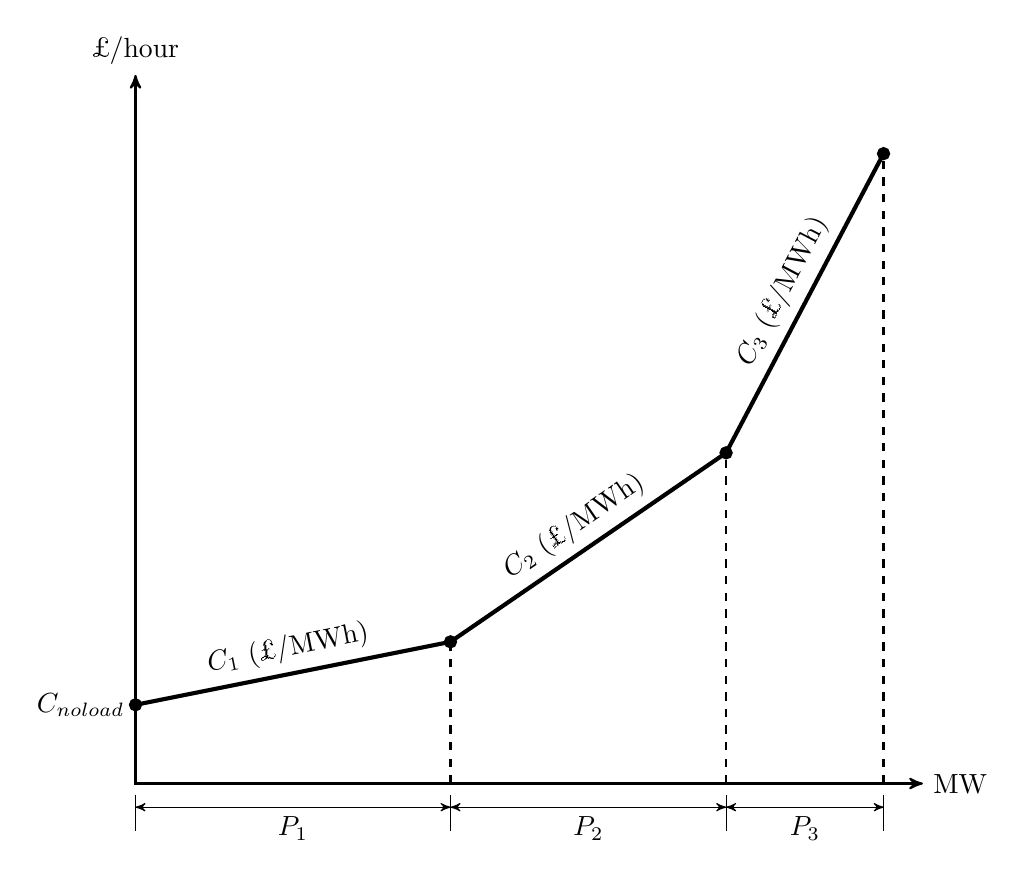
\begin{tikzpicture}[thick]
  \tikzstyle{incr}=[above,sloped,text width=30mm,text centered]

  \coordinate (orig) at (0,0);
  \coordinate (y) at (0,9);
  \coordinate (x) at (10,0);

  \coordinate (p0) at (0,1);
  \coordinate (p1) at (4,1.8);
  \coordinate (p2) at (7.5,4.2);
  \coordinate (p3) at (9.5,8);

  \draw[axis] (y) node[above]{\pounds/hour} -- (orig) -- (x) node[right]{MW};

  \foreach \pnt in {p0,p1,p2,p3}
    \node[circle,draw,minimum width=4pt,inner sep=0pt,fill=black] at (\pnt) {};

%   \draw[line width=1.5pt] (p0) node[left]{$C_{noload}$} --
%   node[incr]{{\small $1^{st}$ incremental price (\pounds/MWh)}} (p1) --
%   node[incr]{{\small $2^{nd}$ incremental price (\pounds/MWh)}} (p2) --
%   node[incr]{{\small $3^{rd}$ incremental price (\pounds/MWh)}} (p3);
  \draw[line width=1.5pt] (p0) node[left]{$C_{noload}$} --
  node[incr]{$C_1$~(\pounds/MWh)} (p1) --
  node[incr]{$C_2$~(\pounds/MWh)} (p2) --
  node[incr]{$C_3$~(\pounds/MWh)} (p3);

  \draw[help lines] (p1 |- x) coordinate (cp1) -- (p1);
  \draw[help lines] (p2 |- x) coordinate (cp2) -- (p2);
  \draw[help lines] (p3 |- x) coordinate (cp3) -- (p3);

  \coordinate (c1) at (intersection of orig--x and p1--cp1);
  \coordinate (c2) at (intersection of orig--x and p2--cp2);
  \coordinate (c3) at (intersection of orig--x and p3--cp3);
  \coordinate (off) at (0,3mm);

%  \fill[red] (c1) circle (2pt);
  \draw[<->,thin] ($(orig)-(off)$) -- node[below]{$P_1$} ($(c1)-(off)$);
  \draw[<->,thin] ($(c1)-(off)$) -- node[below]{$P_2$} ($(c2)-(off)$);
  \draw[<->,thin] ($(c2)-(off)$) -- node[below]{$P_3$} ($(c3)-(off)$);

  \foreach \pnt in {orig,c1,c2,c3}
    \draw[-,thin,shorten <= 4pt] (\pnt) -- ($(\pnt)-2*(off)$);

\end{tikzpicture}
\caption{Pool bid structure.}
\end{figure}


% \begin{figure}
% \label{fig:cost_function}
% \centering
% \begin{Large}
% \begin{tikzpicture}[thick]
% %  \draw[step=1.0cm,color=gray] (0,0) grid (8,5);
% %  \node at (4.5,9.5) {Active power cost function};
%   \coordinate (y) at (0,9);
%   \coordinate (x) at (10,0);
%   \coordinate (p0) at (0,0.1);
%   \coordinate (p1) at (3.2,0.4);
%   \coordinate (p2) at (5.2,1.0);
%   \coordinate (p3) at (7,2.5);
%   \coordinate (p4) at (8.6,5);
%   \coordinate (pn) at (9.5,8.5);
%
%   \foreach \pnt in {p0,p1,p2,p3,pn}
%     \node[circle,draw,minimum width=4pt,inner sep=0pt,fill=black] at (\pnt) {};
%
% %   \draw[axis] (y) -- node[anchor=south,rotate=90,minimum size=15mm]
% %   {Cost \$/MWh} (0,0) -- node[anchor=north,minimum size=15mm] {Set-point (MW)}
% %   (x);
%   \draw[axis] (y) node[above]{$c$} -- (0,0) -- (x) node[right]{$p$};
% %  \coordinate (offprca) at ($0.8*(y)$);
% %  \coordinate (offprcb) at ($0.533*(y)$);
% %  \coordinate (offqtya) at ($.6*(x)$);
% %  \coordinate (offqtyb) at ($.9*(x)$);
% %  \draw[] let \p1=(offprca), \p2=(offqtya) in
% %  (\p1) node[left] {$\alpha$} -- (\p2);
%   \draw[line width=1.5pt] (p0) -- (p1) -- (p2) -- (p3);
%   \draw[line width=1.5pt] (p3) -- ($(p3)!0.6!(p4)$);
%   \draw[dotted] ($(p3)!0.6!(p4)$) -- ($(p3)!1.5!(p4)$);
%   \draw[dashed,line width=1.5pt,shorten >=15pt] ($(p3)!0.6!(p4)$) -- (p4);
%
%   \draw[line width=1.5pt] ($(p4)!0.4!(pn)$) -- (pn);
%   \draw[dotted] ($(p4)!-0.5!(pn)$) -- ($(p4)!0.4!(pn)$);
%   \draw[dashed,line width=1.5pt,shorten >=15pt] ($(p4)!0.4!(pn)$) -- (p4);
%
%   \draw[help lines] (p1 |- x) node[below]{$p_1$} -- (p1) -- (y |- p1)
%   node[left]{$c_1$};
%   \draw[help lines] (p2 |- x) node[below]{$p_2$} -- (p2) -- (y |- p2)
%   node[left]{$c_2$};
%   \draw[help lines] (p3 |- x) node[below]{$p_3$} -- (p3) -- (y |- p3)
%   node[left]{$c_3$};
%   \draw[help lines] (pn |- x) node[below]{$p_n$} -- (pn) -- (y |- pn)
%   node[left]{$c_n$};
%
%   \foreach \x in {2,3.5,5,6.5}
%     \draw[->,line width=2pt] (\x,6.2) -- (\x,5);
%   \node at (4.25,6.2) {$y$};
% \end{tikzpicture}
% \end{Large}
% \caption{Piecewise linear active power cost function and illustration of
% constrained cost variable minimsation, adapted from [ref].}
% \end{figure}

Figure \ref{fig:poolbids} diagrams four of the five price parameters
that made up a bid.  A start-up price would also be stated, representing the
cost of turning on the generator from cold.  The no-load price $c_{noload}$
represents the cost in pounds of keeping the generator running regardless of output. Three
incremental prices $c_1$, $c_2$ and $c_3$ specify the cost in \pounds/MWh of
generation between set-points $p_1$, $p_2$ and $p_3$.

A settlement computer program would calculate an unconstrained schedule
(with no account being taken for the physical limitations of the transmission
system), meeting the forecast demand and requirements for reserve while minimising cost.
Cheapest bids up to the marginal point would get accepted first and the bid
price from the marginal generator would generally determine the system marginal
price for each settlement period.  The system marginal price would determine
the prices paid by consumers and paid to generators, which would be adjusted
such that that the costs of transmission are covered by the market and that the
availability of capacity is encouraged at certain times.

Variations in demand and changes in plant availability got adjusted for by
the grid operator, producing a constrained schedule.  Generators having
submitted bids would be instructed to increase or reduce production
appropriately.  Alternatively, the grid operator could instruct large customers
with contracts to curtail their demand to do so or instruct generators
contracted to provide ancillary services to adjust production.

\subsection{British Electricity Transmission and Trading Arrangements}
%\subsection{New Electricity Trading Arragements}
\label{sec:betta}
Concerns over exploitation of market power in The England and Wales Electricity
Pool and its effectiveness in reducing consumer electricity prices prompted the
introduction of New Electricity Trading Arrangements (NETA) in March 2001
\cite{martoccia:2005}.  The aim was to improve efficiency and provide greater
choice to participants.  Control of the Scottish transmission system was
handed over to England with the introduction of the nationwide British
Electricity Transmission and Trading Arrangments (BETTA) in April 2005 under The Energy
Act 2004.  While The Pool operated a single daily auction and dispatched plant
centrally, under the new arrangements participants became self-dispatching and
market positions became determined through continuous bilateral trading
between generators, suppliers, traders and consumers.

The majority of power is traded under the BETTA through long-term contracts
that are customised to the requirements of each party \cite{kirschen:book}.
These suit participants responsible for large power plants or those purchasing
large volumes of power for many customers.  Sizeable amounts of time and
effort are required for these long-term contracts to be formed and this results
in a high associated transaction cost.  However, they reduce risk for large
players and a degree of flexibility can be provided through option contracts.

Electric power is also traded directly between participants through
over-the-counter contracts that are usually of a standardised form.  Such contracts
typically concern smaller volumes of power and have much lower associated
transaction costs.  Often they are used by participants to refine their market
position ahead of delivery time.

Trading facilities, such as power exchanges, provide a means for participants
to fine-tune their positions further, through short-term transactions for
relatively small quantities of energy.  Modern exchanges are computerised and
accept anonymous offers and bids submitted electronically.  A submitted
offer/bid will be paired with any outstanding bids/offers in the system with
compatible price and quantity values.  The details are then displayed for
traders to observe and to use in subsequent trading.

All bilateral trading must be completed before ``gate-closure'' which is a
point in time, before delivery time, that gives the system operator an
opportunity to balance supply and demand and mitigate potential breaches of
system limits.  In keeping with the UK's free market philosphy, a competitive
spot market \cite{schweppe:spot} is used in the balancing process.  A
generator that is not fully loaded may offer a price at which it is willing to
increase its output by a specified quantity, stating the rate at which it is
capable of doing so.  Certain loads may also offer demand reductions at a
price which can typically be implemeted very quickly.  Longer-term contracts
for balancing services are also struck between the system operator and
generators/suppliers in order to avoid the price volatility often associated
with spot markets.

\section{Electricity Market Simulation}
Previous sections have shown the importance of electricity to
modern societies and have explained how the majority of
electricity supply in the UK is trusted to unadministered bilateral trading
arrangements. Electricity supply involves technology, money, people, natural resources and the environment.  These aspects are all changing
and the discipline must be constantly researched to ensure that systems such as
electricity markets are fit for purpose.  The value of electricity to society
means that it is not feasible to experiment with radical changes to trading
arrangements on real systems.  A practical alternative is to create abstract
mathematical models with sets of simplifying approximations and assumptions
and to find analytical solutions by simulating them using computer programs.

Game theory is the branch of applied mathematics in which behaviour in
strategic situations is captured mathematically.  A common approach to doing
this is to model the system and players as a mathematical optimisation problem.  Optimal
power flow is a classic optimisation problem in the field of electric
power engineering and variants are widely used to research electricity
markets.  In this thesis, optimal power flow forms one part of an
\textit{agent-based} simulation, which is an alternative approach to the
mathematics of games.

\subsection{Optimal Power Flow}
\label{sec:opf}
Nationalised electricity supply industries were for many years planned,
operated and controlled centrally.  A system operator would determine which
generators must operate and the required output of the operating units such
that demand and reserve requirements were met and the overall cost of
production was minimised.  In Electric Power Engineering, this is termed the
\textit{unit commitment} and \textit{economic dispatch} problem.

In 1962 a unit commitment formulation was published with power system
constraints incorporated \cite{carpentier:opf}.  \textit{Optimal power flow} is
this integration of the economic and the power flow aspects of power systems into a
mathematical optimisation problem.  The ability to use optimal power flow to
solve centralised power system operation problems and determine prices in power
pool markets has led to it being one of the most widely studied subjects in
the power systems community.

\subsubsection{Power Flow Formulation}
\label{sec:pf_form}
Optimal power flow derives its name from the \textit{power flow} (or load flow)
steady-state power system analysis technique.  Given sets of generator data,
load data and a nodal admittance matrix, a power flow study determines the
voltage
\begin{equation}
V_i = \vert V_i \vert \angle\delta_i = \vert
V_i\vert(\cos\delta_i + j\sin\delta_i)
\end{equation}
at each node $i$ in the power system from which branch flows may be calculated
\cite{grainger:psa}.

\paragraph{Nodal Admittance Matrix}
The nodal admittance matrix describes the electrical network and its
formulation is dependant upon the transmission line, transformer and shunt
models employed.  Following \cite[p.11]{pserc:mp_manual}, a branch in a power
system nodal representation is typically modelled as a medium length
transmission line in series with a regulating transformer at the ``from'' end.  A nominal-$\pi$ model with total series admittance $y_s = 1/(r_s+jx_s)$ and total shunt capacitance $b_c$ represents the transmission line.  The transformer is assumed to be ideal, phase-shifting and tap-changing, with the ratio between primary winding
voltage $v_{f}$ and secondary winding voltage $N = \tau e^{j\theta_{ph}}$
where $\tau$ is the tap ratio and $\theta_{ph}$ is the phase shift angle.
Figure \ref{fig:branch_model} diagrams this conventional branch model.  From
Kirchhoff's Current Law the current in the series impedance is
\begin{equation}
\label{eq:iseries}
i_s = \frac{b_c}{2}v_t - i_t
\end{equation}
and from Kirchhoff's Voltage Law the voltage across the secondary winding of
the transformer is
\begin{equation}
\frac{v_{f}}{N} = v_t + \frac{i_s}{y_s}
\end{equation}
Substituting $i_s$ from equation (\ref{eq:iseries}), gives
\begin{equation}
\label{eq:vfrom}
\frac{v_{f}}{N} = v_t - \frac{i_t}{y_s} + v_t\frac{b_c}{2y_s}
\end{equation}
and rearranging in terms if $i_t$, gives
\begin{equation}
\label{eq:ito}
i_t = v_s \left( \frac{-y_s}{\tau e^{\theta_{ph}}} \right) +
v_r \left( y_s + \frac{b_c}{2} \right)
\end{equation}
The current through the secondary winding of the transformer is
\begin{equation}
N^*i_f = i_s + \frac{b_c}{2}\frac{v_{f}}{N}
\end{equation}
Substituting $i_s$ from equation(\ref{eq:iseries}) again, gives
\begin{equation}
N^*i_f = \frac{b_c}{2}v_t - i_t + \frac{b_c}{2}\frac{v_{f}}{N}
\end{equation}
and substituting $\frac{v_{f}}{N}$ from equation (\ref{eq:vfrom}) and
rearranging, gives
\begin{equation}
\label{eq:ifrom}
i_s = v_s \left( \frac{1}{\tau^2} \left(y_s + \frac{b_c}{2}\right) \right) +
v_r \left(\frac{y_s}{\tau e^{-j\theta}}\right)
\end{equation}

%\begin{figure}
\centering
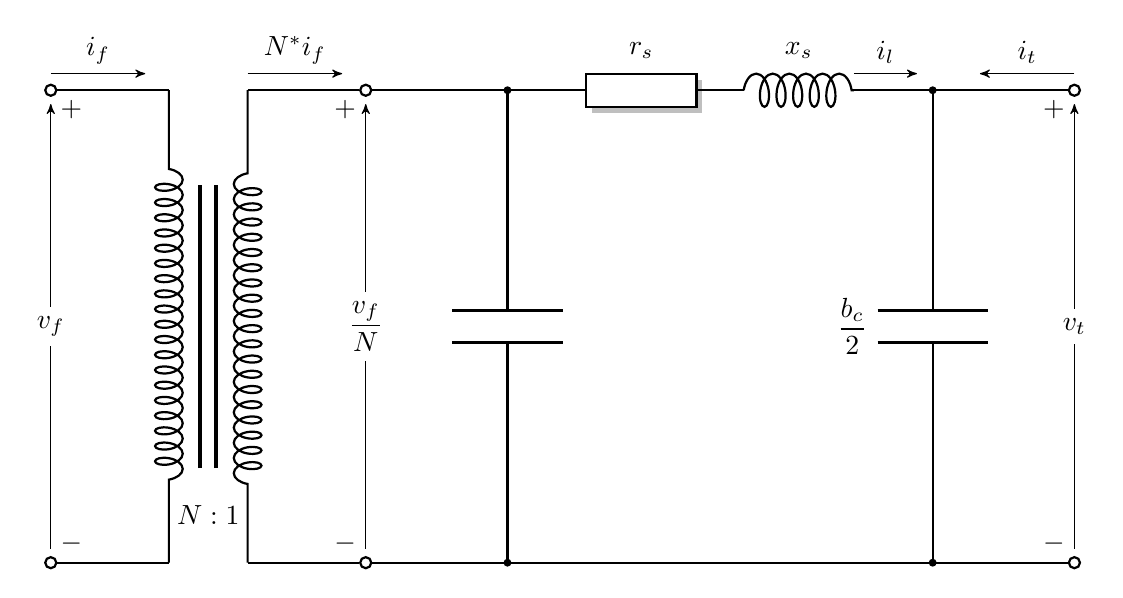
\begin{tikzpicture}[thick]
%   \def\capacitor(#1,#2){%
%     \draw (#1,#2+3cm) -- (#1,#2+5mm);
% %    \draw (#1-1cm,#2+5mm) -- (#1+1cm,#2+5mm);
% %     \draw[linewidth=1pt] (-1cm,-5mm) -- (1cm,-5mm);
% %     \draw[linewidth=1pt] (0,-1cm) -- (0,-5mm);
%   }
%
%   \capacitor(0,0);

%   \def\terminal(#1,#2){#3}{%
%     \node[circle,draw,minimum width=5pt,inner sep=0pt] (#3) at (#1,#2) {};
%   }
%   \terminal(5,5);

  \coordinate (vf0) at (0,0);
  \coordinate (vf+) at (0,6);
  \coordinate (vt0) at (13,0);
  \coordinate (vt+) at (13,6);

  \coordinate (trx) at (2,3);
  \coordinate (vf0p) at ($(trx)-(0.5,3)$);
  \coordinate (vf+p) at ($(trx)+(-0.5,3)$);
  \coordinate (vf0s) at ($(trx)-(-0.5,3)$);
  \coordinate (vf+s) at ($(trx)+(0.5,3)$);

  \coordinate (vl0) at (4,0);
  \coordinate (vl+) at (4,6);
  % resistor
  \coordinate (res) at (7.5,6);
  \coordinate (rin) at ($(res) -(7mm,0)$);
  \coordinate (rout) at ($(res) + (7mm,0)$);
  \coordinate (rh) at (0,6pt);
  % inductor
  \coordinate (ind) at (9.5,6);
  \coordinate (lin) at ($(ind)-(7mm,0)$);
  \coordinate (lout) at ($(ind)+(7mm,0)$);

  \coordinate (capw) at (7mm,0);
  \coordinate (bc1) at (5.8,3);
  \coordinate (bc1in) at ($(bc1) + (0,2mm)$);
  \coordinate (bc1out) at ($(bc1) - (0,2mm)$);
  \coordinate (bc2) at (11.2,3);
  \coordinate (bc2in) at ($(bc2) + (0,2mm)$);
  \coordinate (bc2out) at ($(bc2) - (0,2mm)$);

  \node[circle,draw,minimum width=4pt,inner sep=0pt] (nvf0) at (vf0) {};
  \node[circle,draw,minimum width=4pt,inner sep=0pt] (nvf+) at (vf+) {};
  \node[circle,draw,minimum width=4pt,inner sep=0pt] (nvl0) at (vl0) {};
  \node[circle,draw,minimum width=4pt,inner sep=0pt] (nvl+) at (vl+) {};
  \node[circle,draw,minimum width=4pt,inner sep=0pt] (nvt0) at (vt0) {};
  \node[circle,draw,minimum width=4pt,inner sep=0pt] (nvt+) at (vt+) {};

  \draw (nvl0) -- (nvt0);
  % transformer
  \draw (nvf0) -- (vf0p);
  \draw (vf0s) -- (nvl0);
  \draw (nvf+) -- (vf+p);
  \draw (vf+s) -- (nvl+);
  \draw[decorate,decoration={coil,amplitude=5pt,segment length=5.5pt,
  pre length=10mm,post length=10mm}] (vf+p) -- (vf0p);
  \draw[decorate,decoration={coil,amplitude=5pt,segment length=5.5pt,
  pre length=10mm,post length=10mm}] (vf0s) -- (vf+s);
  \coordinate (cor1) at ($(trx)-(1mm,0)$);
  \coordinate (cor2) at ($(trx)+(1mm,0)$);
  \coordinate (corh) at (0,1.8);
  \draw[line width=1.5pt] ($(cor1)-(corh)$) -- ($(cor1)+(corh)$);
  \draw[line width=1.5pt] ($(cor2)-(corh)$) -- ($(cor2)+(corh)$);

  % resistor
  \filldraw[fill=white,drop shadow] ($(rin)-(rh)$) rectangle ($(rout)+(rh)$);
  \draw ($(res) + (0,5mm)$) node {$r_s$};
  \draw (nvl+) -- (rin);

  \draw (rout) -- (lin);
  % inductor
  \draw[decorate,decoration={coil,amplitude=6pt,segment length=6pt}]
  (lin) -- (lout);
  \draw ($(ind) +(0,5mm)$) node {$x_s$};
  \draw (lout) -- (nvt+);
  % capacitor 1
  \draw (bc1in) -- (bc1in |- vf+s) node[circle,draw,minimum width=2pt,
  inner sep=0pt,fill=black]{};
  \draw (bc1out) -- (bc1out |- vf0s) node[circle,draw,minimum width=2pt,
  inner sep=0pt,fill=black]{};
  \draw[line width=1.2pt] ($(bc1in)-(capw)$) -- ($(bc1in)+(capw)$);
  \draw[line width=1.2pt] ($(bc1out)-(capw)$) -- ($(bc1out)+(capw)$);
%   \draw[line width=1.2pt] ($(bc1out)$) .. controls ($(bc1out)+(capw)+(-2mm,0)$)
%   .. ($(bc1out)+(capw)+(0,-2mm)$); \draw ($(bc1) + (capw)$) node[anchor=west] {$\dfrac{b_c}{2}$};
  % capacitor 2
  \draw (bc2in) -- (bc2in |- vt+) node[circle,draw,minimum width=2pt,
  inner sep=0pt,fill=black]{};
  \draw (bc2out) -- (bc2out |- vt0) node[circle,draw,minimum width=2pt,
  inner sep=0pt,fill=black]{};
  \draw[line width=1.2pt] ($(bc2in)-(capw)$) -- ($(bc2in)+(capw)$);
  \draw[line width=1.2pt] ($(bc2out)-(capw)$) -- ($(bc2out)+(capw)$);
  \draw ($(bc2) - (capw)$) node[anchor=east] {$\dfrac{b_c}{2}$};

  \draw[->,shorten >=5pt,shorten <=5pt,thin] (vf0) node[above right] {$-$} --
  node[fill=white] {$v_f$} (vf+) node[below right] {$+$};
  \draw[->,shorten >=5pt,shorten <=5pt,thin] (vl0) node[above left] {$-$} --
  node[fill=white] {$\dfrac{v_f}{N}$} (vl+) node[below left] {$+$};
  \draw[->,shorten >=5pt,shorten <=5pt,thin] (vt0) node[above left] {$-$} --
  node[fill=white] {$v_t$} (vt+) node[below left] {$+$};
  \node at ($(trx)-(0,2.4)$) {$N:1$};
  \draw[->,thin] ($(vf+)+(rh)$) -- node[above]{$i_f$} ++(12mm,0);
  \draw[->,thin] ($(vf+s)+(rh)$) -- node[above]{$N^*i_f$} ++(12mm,0);
  \draw[->,thin] ($(vt+)+(rh)$) -- node[above]{$i_t$} ++(-12mm,0);
  \draw[->,thin] ($(lout)+(rh)$) -- node[above]{$i_l$} ++(8mm,0);

\end{tikzpicture}
\caption{Nominal-$\pi$ transmission line model in series with a phase
shifting transformer model.}
\label{fig:branch_model}
\end{figure}

Combining equations (\ref{eq:ito}) and (\ref{eq:ifrom}), the \textit{from}
and \textit{to} end complex current injections for branch $l$ are
\begin{equation}
\label{eq:ybranch}
\begin{bmatrix}
i_f^l\\
i_t^l
\end{bmatrix}
=
\begin{bmatrix}
y_{ff}^l& y_{ft}^l\\
y_{tf}^l& y_{tt}^l
\end{bmatrix}
\begin{bmatrix}
v_f^l\\
v_t^l
\end{bmatrix}
\end{equation}
where
\begin{eqnarray}
\label{eq:yff}
y_{ff}^l& =& \frac{1}{\tau^2} \left(y_s + \frac{b_c}{2}\right)\\
\label{eq:yft}
y_{ft}^l& =& \frac{y_s}{\tau e^{-j\theta_{ph}}}\\
\label{eq:ytf}
y_{tf}^l& =& \frac{-y_s}{\tau e^{j\theta_{ph}}}\\
\label{eq:ytt}
y_{tt}^l& =& y_s + \frac{b_c}{2}
\end{eqnarray}
Let $Y_{ff}$, $Y_{ft}$, $Y_{tf}$ and $Y_{tt}$ be $n_l \times 1$ vectors where
the $l^{th}$ element of each corresponds to $y_{ff}^l$, $y_{ft}^l$,
$y_{tf}^l$ and $y_{tt}^l$, respectively.  Furthermore, let $C_f$ and $C_t$ be the
$n_l \times n_b$ branch-bus connection matrices, where $C_{f_{i,j}} = 1$ and
$C_{t_{i,k}} = 1$ if branch $i$ connects from bus $j$ to bus $k$.  The
$n_l \times n_b$ branch admittance matrices are
\begin{eqnarray}
Y_f& =& \diag(Y_{ff})C_f + \diag(Y_{ft})C_t\\
Y_t& =& \diag(Y_{tf})C_f + \diag(Y_{tt})C_t
\end{eqnarray}
and the
$n_b \times n_b$ nodal admittance matrix is
\begin{eqnarray}
Y_{bus}& =& C_f^\mathsf{T} Y_f + C_t^\mathsf{T} Y_t .
\end{eqnarray}
% and it relates the complex bus voltages to the nodal current injections
% \begin{eqnarray}
% I_{bus}& =& Y_{bus}V
% \end{eqnarray}
% The complex bus power injections are expressed as a non-linear function of $V$
% \begin{eqnarray}
% S_{bus}(V)& =& \diag(V)I_{bus}^* \nonumber \\
% \label{eq:sbus}
% &= & \diag(V)Y_{bus}^*V^*
% \end{eqnarray}
% The net complex power injection (generation - load) at each bus must equal the
% sum of complex power flows on each branch connected to the bus.  Hence the AC
% power balance equations are
% \begin{equation}
% \label{eq:mismatch}
% S_{bus}(V) + S_d - S_g = 0
% \end{equation}

\paragraph{Power Balance}
% Importantly, the relationship between nodal voltages and power entering the
% network is non-linear.
For a network of $n_b$ nodes, the current injected at
node $i$ is
\begin{equation}
I_i = \sum_{j=1}^{n_b} Y_{ij} V_j
\end{equation}
where $Y_{ij} = \vert Y_{ij}\vert \angle\theta_{ij}$ is the $(i,j)^{th}$ element
if the $Y_{bus}$ matrix.  Hence, the apparent power entering
the network at bus $i$ is
\begin{equation}
S_i = P_i+Q_i = V_iI_i^* = \sum_{n=1}^{n_b} \vert Y_{ij}V_iV_j \vert \angle
(\delta_i - \delta_j - \theta_{ij})
\end{equation}
Converting to polar coordinates and separating the real and imaginary parts,
the active power
\begin{equation}
P_i = \sum_{n=1}^{n_b} \vert Y_{ij}V_iV_j \vert \cos(\delta_i - \delta_j -
\theta_{ij})
\end{equation}
and the reactive power entering the network
\begin{equation}
Q_i = \sum_{n=1}^{n_b} \vert Y_{ij}V_iV_j \vert \sin(\delta_i - \delta_j -
\theta_{ij})
\end{equation}
at bus $i$ are non-linear functions of $V_i$, as indicated by the presence of
the sine and cosine terms.  Kirchoff's Current Law requires that the net
complex power injection (generation - load) at each bus equals the sum of
complex power flows on each branch connected to the bus.  The power balance
equations
\begin{equation}
\label{eq:p_balance}
P_g^i - P_d^i = P^i
\end{equation}
and
\begin{equation}
\label{eq:q_balance}
Q_g^i - Q_d^i = Q^i
\end{equation}
where the subscripts $g$ and $d$ indicate generation and demand
respectively, form a key non-linear constraint in the optimal power flow
problem.

\subsubsection{Optimal Power Flow Formulation}
Optimal power flow is a mathematical optimisation problem in which the complex
power balance equations (\ref{eq:p_balance}) and (\ref{eq:q_balance}) form one
of the constraints. Mathematical optimisation problems have the general form
\begin{equation}
\min_x f(x)
\end{equation}
subject to
\begin{eqnarray}
\label{eq:equality}
g(x)& =& 0\\
\label{eq:inequality}
h(x)& \leq& 0
\end{eqnarray}
where $x$ is the optimisation variable, $f$ is the objective function and
equations (\ref{eq:equality}) and (\ref{eq:inequality}) are sets of equality
and inequality constraints on $x$, respectively.  Typical inequality
constraints are bus voltage magnitude contingency state limits, generator
output limits and branch power or current flow limits.  The optimisation
variable $x$ may be made up of generator set-points, bus voltages, transformer
tap settings etc.  If the optimisation variable $x$ is empty then the
formulation reduces to the general power flow problem described in above.

A common objective of optimal power flow is total system cost minimisation.
For and network of $n_g$ generators the objective function is
\begin{equation}
\min_{\theta, V_m, P_g} \sum_{k=1}^{n_g} C_k(P_{g,k})
\end{equation}
where $C_k$ is a cost function (typically quadratic) of the set-point $P_{g,k}$
for generator $k$.  Alternative objectives may be to minimise losses, maxmimise
the voltage stability margin or minimise deviation of an optimisation variable
from a particular schedule \cite[\S18]{kallrath:2009}.

\subsubsection{Interior-Point Methods}
Many solution methods for optimal power flow have been developed in the
years since Carpienterm introduced the concept and the majority are reviewed
in \cite{momoh:part1,momoh:part2}.  Interior point methods have proven to be
particularly robust and solve the Lagrangian function
\begin{equation}
\mathcal{L}(x) = f(x) + \lambda^\mathsf{T}g(x) + \mu^\mathsf{T}h(x)
\end{equation}
where $\lambda$ and $\mu$ are the Lagrangian multipliers.

\subsection{Agent-Based Simulation}
Social systems, such as electricity markets, are inherently complex and involve
interactions between different types of individuals and between individuals
and collective entities, such as organisations or groups, the behaviour of which
is itself the product of individual interactions.  This complexity
drives classical monolithic equilibrium models to their limits.  Models are
often highly stylised and limited to small numbers of players with strong
constraining assumptions made about their behaviour.

Agent-based simulation involves modelling simultaneous operations and
interactions between adaptive agents and assessing their effect on the system
as a whole.  Macro-level system properties arise from agent interactions, even
those with simple behavioural rules, that could not be deduced by simply
aggregating the agent's properties. % Game of Life

Following \cite{tesfatsi:handbook}, the objectives of agent-based modelling
research fall roughly into four strands: empirical, normative, heuristic and
methodological. The \textit{empirical} objectives are to understand how and why macro-level
regularities have evolved from micro-level interactions when little or no
top-down control is present.  Reaserch with \textit{normative} goals aims to
relate agent-based models to an ideal standard or optimal design.  The objective being
to evaluate proposed designs for social policy, institutions or processes in
their ability to produce socially desirable system performance.  The
\textit{heuristic} strand aims to generate theories on the fundamental causal
mechanisms in social systems that can be observed, even in simple systems, when there are
alternative initial conditions.  This thesis aims to provide
\textit{methodologial} advancement in the field.  Improvements in the tools
and methods available aid research with the former objectives.

\section{Summary}


% Survey and critical assessment. Relation to own work.
\chapter{Related Work}
\label{ch:related_work}
This thesis concerns methodological advancement in the field of agent-based
electricity market simulation.  This chapter describes the research in the
context of similar work with particular emphasis on the methods employed.  The
bulk of the review focuses upon agent-based simulation with decision models
based upon reinforcment learning.  However, simulations applying alternative
methods, such as genetic algorithms and learning classifier systems, are also
surveyed.  In the interests of repeatability, the software developed for
this thesis has been released as open source and the project is described in
the context of other open source electric power engineering tools.

\section{Policy Gradient Reinforcement Learning}
Direct policy search reinforcement learning methods have been sucessfully
applied to financial decision making problems.  It is more common for
supervised learning techniques to be trained on sample data and used to
minimise errors in price forecasts.  However, in \cite{moody:98} a recurrent
reinforcement learning method is used to optimise investment performance
without forecasting prices.  The method is recurrent as it uses information
related to past decisions as input.  The authors compare using direct profit
and the Sharpe ratio \cite{sharpe:ratio66,sharpe:ratio94} as a reward signal.
The Sharpe ratio is a measure of isk adjusted return defined as
\begin{equation}
S_t = \frac{\mbox{Average}(R_t)}{\mbox{Standard Deviation}(R_t)}
\end{equation}
where $R_t$ is the return for period $t$.
% The parameters of the trading system $\theta$ are adjusted in the direction of
% the gradient $\partial S_t / \partial \theta_t$.

The trading system parameters $\theta$ are updated in the direction of the
steepest accent of the gradient of some performance function $U_t$ with repect
to $\theta$
\begin{equation}
\Delta\theta_t = \rho \frac{dU_t(\theta_t)}{d\theta_t}
\end{equation}
where $\rho$ is the learning rate.  Direct profit is the simplest performance
function defined, but assumes traders are insensitive to risk.  Investors
being, in general, sensitive to losses are willing to sacrifice potantial gains
for reduced risk of loss.
To allow on-line learning and parameter updates at each time period, the
authors define a \textit{differential} Sharpe ratio.  By maintaining an
exponential moving average of the Sharpe ratio, the need to compute return
averages and standard deviations for the entire trading history at each period
is avoided.  Alternative performance ratios including the \textit{information
ratio}, \textit{appraisal ratio} and \textit{Sterling ratio} are mentioned.

Simulations are conducted using artificial price data, equivalent to one year
of hourly trade in a 24-hour market, and 45 years of monthly data from the
Standard \& Poor (S\&P) 500 index and 3 month Treasury Bill (T-Bill) data. In a
portfolio management simulation, in which trading systems invested proportions
of their wealth among three different securities, it was shown that trading
systems maximising the differential Sharpe ratio produced more consistent
results and achieved higher risk adjusted returns than those trained to simply
maximise profit.  This result is interesting as the majority of applications of
reinforcement learning to electricity market simulation use profit as a reward
signal and may benefit from using measures of risk adjusted return.

In \cite{moody:direct} the recurrent reinforcement learning method from
\cite{moody:98} is contrasted with value function based approaches.  In
addition to the Sharpe ratio, the \textit{Downside Deviation} ratio is
described and may also be of use in electricity market simulation.  Simulation
results from trading systems trained on half-hourly USD/GBP foreign exchange
rate data and again learning switching strategies between the S\&P 500 stock
index and T-Bills are presented.  The results show that the recurrent
reinforcement learning method outperforms the Q-learning in the S\&P 500/T-Bill
allocation problem.  The authors also observe that the recurrent reinforcement
learning method has a simpler functional form, the output is not discrete and
easily maps to real valued actions and that the algorithm is more robust to
noise in financial data and adapts quickly to non-stationary environments.

In \cite{vengerov:grid} a marketplace for computational resources in
envisioned.  The authors propse a market in which grid service suppliers offer
to execute jobs submitted by customers for a price per CPU-hour.  The problem
formulation requires customers to request a quote for computing a job $k$ for a
time $\tau_k$ on $n_k$ CPUs.  The quote returned specifies a price $P_k$ at
which the $k$ would be charged and a delay time $d_k$ for the job.  The service
provider's goal is to learn a policy for pricing quotes that maximises long
term revenue when competing in a market environment with other providers.  A
differentiated pricing model is implemented where a standard service is priced
at 1~\$/CPU-hour and a premium sercice a $P$~\$/CPU-hour, with premium jobs
prioratised over standard jobs.  The state of the market environment is defined
by the current expected delays in the standard and premium service classes and
the product of the number of CPUs requested and the job execution time,
$n_k \tau_k$.  The reward $r(s,a)$ for action $a$ in state $s$ is the total
price paid for the job.  The policy gradient method employed is a modified
version of Williams' REINFORCE where
\begin{equation}
Q(s_t,a_t) = \sum_{t=1}^T r(s_t,a_t) - \overline{r}_t
\end{equation}
and $\overline{r}_t$ is the current average reward.

The authors recognise that their grid market model could be applied to any
multi-seller retail market environment.  The experimental results show that if
all grid service providers simultaneously use the learning algorithm then the
process converges to a Nash equilibrium.  The results also showed that
significant increases in profit were possible by offering both standard and
premium services.

% \section{Agent-Based Simulation}
% Relative to the traditional closed-form equilibrium approaches, agent-based
% simulation of (electricity) markets is a new field of research.  For
% comprehensive reviews and surveys of the many different techniques that have
% been applied in recent years the interested reader is directed to
% \cite{weidlich:08,tesfatsi:handbook,visud:thesis}.  This section will focus on
% reviewing literature from the field in which reinforcement learning techniques
% were applied in combination with explicit power system models.  A short review
% is also provided of some more general applications of reinforcement learning
% with connectionist systems and policy-gradient methods.

% Game theoretic models are commonly associated with economics and attempt to
% capture behaviour in strategic situations mathematically.  They have been
% applied to electric energy problems of many forms, including but not limited
% to analysis of market structure, market liquidity, pricing methodologies,
% regulatory structure, plant positioning and network congestion.  More
% recently, agent-based simulation has received a certain degree of attention
% from researchers and has been applied in some of these fields also.
%
% While popular and seemingly promising, agent-based simulation is still centred
% around abstracted models.  The assumptions made is this abstraction must be
% subjected to the same verification and validation as with equation-based
% models.  Verification of assumptions and model validation are often overlooked
% in agent-based simulations of energy markets, yet they are possibly the most
% important steps in the model building process.  Techniques used to develop,
% debug and maintain large computer programs can often be used to verify that a
% model does what it is intended to do.
%
% Validation of an energy market model is more difficult.  It can be accomplished
% using the intuition of experts or through comparison of simulation results
% with either historical market data or theoretical results from more abstract
% representations of the model.  Finding verifyable trends in existing markets
% is a very large challenge.  To then prove that a computational model
% replicates these characteristics with suitable fidelity is yet more
% challenging still.  Only when a model is suitably verified and validated can
% any conclusions be drawn from results obtained through implementation and
% simulation of suitable scenarios.

\section{Simulations Applying Q-learning}
% Krause et al.\ have published agent-based energy market research in which
% Q-learning methods were applied while considering physical system properties.
% In a comparison between Nash equilibrium analysis and agent-based simulation,
% the suitability of bottom-up modelling for the assessment of market evolution
% was assessed\cite{krause:nash}.  This is built upon in subsequent publications
% which evaluate the influence on market power and social welfare of three
% congestion management schemes and which analyse strategic behavior in combined
% gas and electricity markets\cite{krause:cong,krause:gas}.  Power Transmission
% Distribution Factors (PTDF) are used in place of explicit power flow equations
% in determining line flows.  The action domain of generating agents is limited
% to 0\%, 5\% and 10\% markups on true marginal costs.  The implementation of the
% Q-learning method used does not differentiate between environment states when
% selecting actions. This is a modification to the traditional formulation that
% still results in convincing conclusions, as with the popular Roth-Erev method.
%
% There are similar applications of Q-learning in which states \textit{are}
% defined, but none model the AC transmission system.  A common approach is to
% use categorised market price from the previous period as state
% information\cite{bakirtzis:psce,xiong:discrim}.
Agent-based simulation of electricity markets has been researched with
participants behavioral aspects modelled using Q-learning methods.  The most
prominent work in which this method has been is adopted has been conducted at
the Swiss Federal Institutes of Technology in Zurich and Lausanne.  The
foundations for this were laid in \cite{krause:nash04} with a
comparison of agent-based modelling using reinforcement learning with Nash
equilibrium analysis in assessing network constrained power pool market
dynamics.  Parameter sensistivity of comparison results were later analysed in
\cite{krause:nash06}.

In the papers a mandatory spot market is modelled and cleared using a DC
optimal power flow formulation.  A five bus power system model is defined with
three generators and four inelastic and constant loads.  Linear marginal cost
functions
\begin{equation}
C_{g,i}(P_{g,i}) = b_{g,i} + s_{g,i}P_{g,i}
\end{equation}
are assumed for each generator $i$ where $P_{g,i}$ is the active power output,
$s_{g,i}$ is the slope of the cost function and $b_{g,i}$ is the cost when
$P_{g,i} = 0$.  Suppliers are given the option to markup their bids to the
market not by increasing the slope, but by increasing $b_{g,i}$ by 10\%, 20\%
or 30\%.  A price cap of \$60/MW is set, but may not be exceeded by any of the
available markups.

Nash equilibrium of the market is computed by clearing the market for all
possible markup combinations and determining the actions for which no player is
motivated to deviate from as it would result in a decrease in expected reward.
Experiments are conducted in which there is a single Nash equilibrium and two
equilibria.

An $\epsilon$-greedy strategy is applied for action selection and a stateless
action value function is updated at each time step $t$ according to
\begin{equation}
Q(a_t) \leftarrow Q(a_t) + \alpha(r_{t+1} - Q(a_t))
\end{equation}
where $\alpha$ is the learning rate.  Further to \cite{krause:nash04},
simulations with discrete sets of values for the parameters $\alpha$ and
$\epsilon$ were carried out in \cite{krause:nash06}.  While parameter
variations affected the frequency of equilibrium oscillations, Nash equilibrium
was still approached and the oscillatory behaviour observed for almost all
combinations.

The significance of this research is that is verifies that the agent-based
approach settles at the same theoretical optimum as with closed-form equilibrium
approaches and that exploratory policies result in the exploitation of multiple
equlibria if they exist.


Having validated the suitability of an agent-based, bottom-up, approach to
assessing evolution of market characteristics, the authors applied the technique
in a comparison of congestion management schemes \cite{krause:cong}.  The first
scheme considered was \textit{locational marginal pricing}, or nodal pricing,
where congestion is managed by optimising the output of generators with respect to
maximum social welfare.  Loading of branches to their flow limits results in
non-uniform nodal marginal prices.  A nodal marginal price equals the
increase in the total system cost (the value of the objective function) when
generation at that node is increased by 1MW.  These prices are commonly used in
electricity market analysis as they may be determined from the Lagrangian
multipliers on the active power balance constraints in the optimal power flow
formulation.  The second scheme considered, named \textit{market splitting}, is
similar to locational marginal pricing, but the system gets subdivided into
zones within which the nodal prices are uniform.  The final \textit{flow based
market coupling} scheme also uses uniform zonal pricing, but requires a
simplified representation of the network.  Power flows within zones are not
represented and all lines within zones are aggregated into one equivalent
interconnector.

In a simpler alternative to the conventional DC optimal power flow formulation,
the computation of line power flows is done using a matrix power transfer
distribution factors.  The $(i,j)^{th}$ element of this matrix corresponds to
the change in active power flow on line $j$ given an additional injection of
1MW at the slack bus and corresponding withdrawl of 1MW at node $i$.

The congestion management schemes are evaluated under perfect competition, where
suppliers bid at marginal cost, and under oligopolistic competition, in which
markups of 5\% and 10\% may be added to marginal cost.  The benefits obtained
between reward at marginal cost and a maximum markup are used to assess market
power.  The experimental results show different market power allocations under
the three constraint management schemes.  The significance of this work is that
it demonstrates an agent-based model being applied to an important problem in
the electricity supply industry.

The same Q-learning method is used in \cite{krause:gas} to analyse strategic
behaviour in integrated electricity and gas markets.  Again, power flow are
modelled using a power transfer distribution matrix.  Pipeline losses in the
gas network are approximated using using a cubic function of the flow.  Three
combined gas and electricity models are compared.  In the first model,
operators of gas-fired power plant submit separate bid functions for gas and
electricity.  Bids are then cleared as a single optimisation problem.  In model
two, operators submit one offer for their capacity to convert gas to
electricity.  In the final model, bids are submitted only to the electricity
market, after which gas is purchased regardless of price.  Gas supply offers are
modelled as a linear function with no strategic involvement.  The models are
compared in terms of social welfare using a three bus power system model with
three non-gas-fired power plants and one gas-fired plant.  The experimental
results show little difference between electricity prices and social welfare
prices between the models.

However, this research illustrates the interest in and complexity associated
with modelling relationships between markets.  The authors recognise the need
for further and more detailed simulation in order to improve evaluation of
market coupling models.


Researchers at the Argonne Nationa Laboratory have published results from a
preliminary study of interactions between \textit{emission} and electricity
markets \cite{wang:09}.  A cap-and-trade system for emissions is modelled where
generator companies are allocated with $\mbox{CO}_2$ allowances that may
subsequently be traded.  Generator companies are assumed to be price takers in
the emissions market and to have negligible influence on market clearing
prices. Prices for allowances from the European Energy Exchange were used.
Whereas in the electricity market, an oligopoly is assumed and bids are cleared
using a DC optimal power flow formulation.  To improve selection of the
$\epsilon$ parameter for exploratory action selection, a simulated annealing
(SA) Q-learning method based on the Metropolis criterion is used \cite{guo:sa}.
Under this method $\epsilon$ is changed at each simulation step to allow
solutions to escape from local optima.  A two bus system is used to study cases
in which, allowance trading is not used, allowances can be exchanged in the
emission market and with variations in the allowance allocations.

A one year, hourly load profile with a summer peak is used to represent changes
in demand.  The electricity market is cleared each hour and the emissions market
at the end of each simulated week.  The agents learn, when they have a defecit
of allowances, to borrow future allowances in the summer when load and
allowance prices are high.  Conversly, when they have a surplus they learn to
sell at this time.  In the third case, the authors show the sensitivity of
profits to initial allocations and conclude that the experimental results can
not be generalised.  The authors cite further model validation and agent
learning method improvements as necessary future work.

The SA-Q-learning method is also used by researchers from the University of
Thessaloniki in \cite{tellidou:tacit} to study capacity withholding and tacit
collusion among electricity market participants.  A mandatory spot market is
implemented, where bid quantities may be less than net capacity and bid prices
may be marked up upon marginal cost by increasing the slope of a linear cost
function.  Again market clearing is achieved using DC optimal power flow and
locational marginal prices are used to calculate profits and reinforce the
learning process.  Demand is assumed to be inelastic and transmission
system parameters constant between simulation periods.  A simple two node
power system model with two generators is used in three test cases.  In a
reference case each generator bids full capacity at marginal cost.  In the
second case, generators bid quantities in steps of 10MW and price markups in
steps of \euro{2}/MWh.  In the final case the same generation capacity is
split among eight identical generators to increase the level of competition.  the
experimental results show that generators learn to withhold capacity and develop
tacit collusion strategies to capture congestion profits.

The convergence to Nash equilibrium shown in \cite{krause:nash04} is confirmed
in \cite{sistani:06}.  Boltzman (soft-max) exploration is used for action
selection with the temperature parameter adjusted during the simulations.  A
modified version of the IEEE 30 bus test system is used with the number of
generators reduced from nine to six.  No optimal power flow formulation or
details of the reward signal are provided.  Generators are given a three step
action space where the slope of a linear supply function may be less then, equal
to or above marginal cost.  The experimental results show that with temperature
parameter adjustment Nash equilibrium is achieved and oscillation associated
with $\epsilon$-greedy action selection are avoided.


\section{Simulations Applying Roth-Erev}
A reinforcement learning method based on empirical results obtained from
observing how humans learn decision making strategies in games against multiple
strategic players has received considerable attention from the agent-based
electricity market simultaion community \cite{roth:games,roth:aer}.

In \cite{nicolaisen:2001} an agent-based model of a wholesale electricity market
with both supply and demand side participation is constructed.  It is used to
study market power and short-run market efficiency under discriminatory pricing
through systematic variation of concentration and capacity conditions.  To model
the power system, each trader is assigned values of available transmission
capability (ATC) with respect to each other trader.  Offers from buyers and
sellers are matched on a merit order basis, with quantities restricted by
the ATCs.  Two issues with the original Roth-Erev method are observed and the
modified version defined in Section \ref{sec:variant} above is proposed.

A maximum markup (markdown) of \$40/MWh is specified for each seller (buyer).
Traders are not permitted to make negative profits and the feasible price range
is divided into 30 offer prices for 1000 auction rounds cases and 100 offer
prices for 10000 aution round cases.  The parameters of the Roth-Erev method are
calibrated using direct search within reasonable ranges.  Nine combinations of
buyer and sellers numbers and total trading capacities are tested using the
calibarated values and \textit{best-fit} parameter values determined by Erev \&
Roth.

The experimental results show that good market efficiency is achieved under all
configurations and the sensitivity to method parameters is small.  Levels of
market power are found to be strongly predictive and little difference is found
between cases in which opportunistic price offers are permitted and when traders
are forced to bid at marginal cost.  The results are compared with those from
\cite{nicolaisen:2000}, in which genetic algorithms were used.  The authors
conclude that the reinforcement learning approach leads to higher market
efficiency due their adaption according to \textit{individual} profits.

Further research from Iowa State University, involving the modified Roth-Erev
method, has centered around the AMES wholesale electricity market test bed.  A
detailed description of which is provided in Section \ref{sec:ames} below.

In \cite{tesfatsi:psce} AMES is used to investigate strategic capacity
withholding in a wholesale electricity market design proposed by U.S. Federal
Energy Regulatory Commission in April 2003.  A five bus power system model with
five generators and three dispatchable loads is defined and capacity withholding
is represented by premitting traders to lower than true operating capacity and
higher than true marginal costs.

Comparing results from a benchmark case (in which true production costs are
reported, but higher than marginal cost functions may be reported) and cases in
which reported production limits may be less than the true values, the authors
find, that with sufficient capacity reserve, no evidence to suggest potential
for inducing higher net earnings through capacity withholding in the WPMP.

Researchers from the University of Genoa have used the modified Roth-Erev
method to study strategic behaviour in the Italian wholsale electricity market
\cite{cincotti:09}.  The exact clearing procedure is replicated and a model of
the Italian transmission system, including an interconnector to Sicily, with
zonal subdivision, is defined.  Within each of the 11 zones, thermal plant is
combined according to technology (coal, oil, combined cycle gas, turbo gas and
repower) and associated with one of 16 generation companies according to the
size of the companies share.  The resulting 53 agents are assumed to bid full
capacity and may markup bid prices in steps of 5\%, with a maximum markup of
300\%.  Bids are cleared using a DC optimal power flow formulation with
generation capacity constraints and zone interconnector flow limits.  Agents are
rewarded according to a uniform national price, computed as a weighted average
of zonal prices with respect to zonal load.  Using actual hourly load data, it
is shown that in experiments in which agents \textit{learn} their optimal
strategy, histrorical trends were replicated in all but certain hours of peak
load.  The authors state a desire to test different learning methods and perform
further empirical validation.

In \cite{micola:08} a multi-tier model of wholesale natural gas, wholesale
electricity and retail electricity markets is studied using another variant of
the Roth-Erev method.  Coordination between strategic business units (SBU)
within the same firm, but participating in different markets, is varied
systematically and profit differences observed.

An initial two-tier model involves firms with two associated agents rewards,
$r^1$ and $r^2$, are initially independant.  A \textit{reward independance}
parameter $\alpha$ is used to control the fraction of profit from the other
market that is used in rewarding the agent.  The total rewards are
\begin{equation}
R^1(t) = (1-\alpha)r^1(t) + \alpha r^2(t)
\end{equation}
and
\begin{equation}
R^2(t) = (1-\alpha)r^2(t) + \alpha r^1(t)
\end{equation}
Each action $a$ is a single price bid between zero and the price from the
preceeding market.  The Roth-Erev method is modified such that similar
actions, $a-1$ and $a+1$, are reinforced also.  For each agent, the action
selection propensities in auction round $t$ are
\begin{equation}
p^i_a(t) = \begin{cases}
(1-\gamma)p^i_a(t-1) + R^i(t)& \text{if $s=k$}\\
(1-\gamma)p^i_a(t-1) + (1-\delta)R^i(t)& \text{if $s=k-1$ or $s=k+1$}\\
(1-\gamma)p^i_a(t-1)& \text{if $s\neq k-1$, $s\neq k$ or $s\neq k+1$}
\end{cases}
\end{equation}
where $\delta$, with $0\leq \delta \leq 1$, is the \textit{local
experimentation} parameter, $\gamma$ is the discount parameter and $i\in \lbrace
1,2 \rbrace$.  Actions whose probability of selection fall below a specified
value are removed from the action space.

The initial simulation consists of two wholesalers and three retailers and
$\alpha$ is varied from $0$ to $0.5$ in $51$ discrete steps.  The experiment
is repeated using a three tier model in which two natural gas shippers supply
three electricity generators who sell to four electricity retailers.  The
results show a rise in market prices as reward interdependance is increased and
greater profits for integrated firms.

In \cite{weidlich:06} the modified Roth-Erev method is used to study
interrelationships between contracts markets and balancing markets.  Bids on the
day-ahead contracts market consist of a price and a volume, which are assumed to
be the same for each hour of the day.  Demand is assumed to be fixed and
inelastic.  Bids on the balancing market consist of a reserve price, a
\textit{work} price and an offered quantity.  The reserve price is that which
must be paid for the quantity to be kept on standby and the work price must be
paid if that quantity is called upon for transmission system stabilisation.  No
optimal power flow formulation or power system model is defined.  At the
day-ahead stage contract market and balancing market (according to reserve
price) bids and are cleared by stacking in order of ascending price until the
forecast demand is met.  On the following day, accepted balancing bids are
cleared according to work price such that requirements for researve dispatch
are met.  Bid prices on the contracts market are stratified into 21 discrete
values between 0 and 100 and bid quantities into six discrete values between 0
and maximum capacity, giving 126 possible actions.  Bid quantities on the
balancing market are equal to the capacity remaining after contract market
participation.  21 discrete capacity prices between 0 and 500 and 5 work prices
between 0 and 100 are permitted, giving 105 possible actions in the balancing
market.  Separate instances of the modified Roth-Erev method are used to learn
bidding strategies for each agent in each of the markets.

Interrelationsships between the markets are studied using four scenarios in
which the order of market execution and the balancing market pricing mechanism
(discriminatory or pay-as-bid) are changed.  Clearing prices in the market
executed first are shown to have a considerable effect on prices in the
following market.  The authors find agent-based simulation to be a suitable
tool for reproducing realistic market outcomes and recognise a need for more
detailed models with larger action domains.

In the same year, the authors collaborated with Jian Yao and Shnuel Oren from
the University of California to study the dynamics between two settlement
markets using the modified Roth-Erev method.  The markets are a forwards
contract market, in which transmission constraints are ignored, and a spot
market that is cleared using a DC optimal power flow formulation with line
flows calculated using power transfer distribution factors.  Zonal prices are
set in the forward market as weighted averages of nodal prices with repect to
historical load shares.  Profits are dtermined using these zonal prices and
nodal prices from optimisation of the spot market.  Demand is assumed
inelastic to price, but different contingency states with peak and low demand
levels are examined.  A 53 bus stylised model of the Belgian electricity
system from \cite{yao:07,yao:08} is used to validate the results against those
obtained using equilibrium methods.  The nineteen generators are divided among
two firms which learn strategies for bid price and quantity selection using the
modified Roth-Erev method with a set of fixed parameter values taken from
\cite{roth:aer}.  The results show that the presence of a forward contracts
market produces lower overall electricity prices and lower price volatility.
The authors mention risk aversion to be included in suppliers utility
functions in future work.

% \subsection{Learning Method Comparisons}
% \subsection{Heuristic Approaches}
% \section{Simulations Applying Genetic Algorithms}
% \section{Learning Classifier Systems}

% \section{Closed-Form Equilibrium}
% Hobbs, Neuhoff

% \section{Policy-Gradient Reinforcement Learning}
% TD-Gammon

\section{Open Source Electric Power Engineering Software}
\label{sec:oss}
In order to couple exisiting implementations of policy gradient reinforcement
learning methods from the PyBrain machine learning library with scalable and
extensible optimal power flow formulations, the
MATLAB\footnote{MATLAB is a registered tradeamark of The Mathworks, Inc.}
source code from MATPOWER was translated to the Python programming language.
With permission from the MATPOWER developers, the resulting package has been
released under the terms of the GNU General Public License (GPL) as a project
named PYLON \cite{lincoln:pyreto}.   This section describes the project in the
context of other open source electric power engineering software and
demonstrates the contribution made.

\subsection{MATPOWER}
Since 1996, a team of researhers at the Power Systems Engineering Research
Center at Cornell University have been developing MATPOWER -- a package of
MATLAB workspace files for solving power flow and optimal power flow problems.
Initial developement was part of the PowerWeb project which is a power
exchange auction market simulator that is accessed by multiple users
simultaneously through a web interface.  MATPOWER is designed to be easy to use
and modify while also offering good performance.  It is available under a
custom license that permits it to be used for any purpose providing the project
and authors are cited.  MATPOWER is very popular in education and research and
an active mailing list is maintained by Ray Zimmerman.

MATPOWER includes five power solvers for both AC and DC problems.  The default
solver uses Newton's method \cite{tinney:67} with the full Jacobian matrix
updated at each iteration.  Two variations on the fast decoupled method
\cite{stott:74} described in \cite{amerongen:89} provide faster convergence in
certain networks.  The standard Gauss-Seidel method \cite{glimn:57} is provided
largely for academic reasons and the DC solver provides non-iterative
method.  The properties of MATLAB sparse matrices are exploited, allowing the
solvers to scale well to very large systems.  All functions are run from the
MATLAB command line or from within users programs and no graphical user
interface is provided.

Starting with the first beta release of version 4.0, MATPOWER includes a pure
MATLAB primal dual interior point method (PDIPM) that can be used for solving
DC and AC optimal power flow problems \cite{zimmerman:ccv}.  Previously,
FMINCON from the MATLAB Optimization Toolbox\footnote{Optimization Toolbox is a registered trademark
of The Mathworks, Inc.} was required or one of a suite of high performance
closed-source solvers.  TSPOPF is a collection of three AC optimal power flow
solvers, implemented in the C programming language and released as MATLAB MEX
files.  It includes the original implementation of the step-controlled PDIPM
from which the pure MATLAB version was derived.  MINOPF provides an interface
to the Fortran based MINOS\footnote{MINOS is trademark of Stanford Business
Software, Inc.} solver developed at the Systems Optimization Laboratory at
Stanford University and is often the fastest solver for MATPOWER, but is
available only for educational and research purposes.  DC optimal power flow
problems can alternatively be solved using a MEX interface to BPMPD -- a
commercial interior point method for linear and quadratic programming.

MATPOWER has an \textit{extensible} optimal power flow formulation that allows
additional optimisation variable and problem constraints to be introduced by
the user.  The is used internally to extend the standard optimisation problem
to supprt piecewise linear cost functions, dispatchable loads, generator PQ
capability curves and branch angle difference limit constraints.  Examples of
additional extensions include: reserve requirements, environmental costs and
contingency constraints.

MATPOWER currently requires MATLAB, version 6.5 or greater, which is a
commercial software product from The Mathworks, Inc that is supported on all
major platforms.  However, with the recent inclusion of a native PDIPM it
should be possible to run MATPOWER on GNU/Octave with minimal alteration.

\subsection{MATDYN}
MatDyn is an extension to MATPOWER developed by Stijn Cole from the Katholieke
Universiteit Leuven for dynamic analysis of electric power systems.  It has
been released under the same license as MATPOWER and has the same style of
code.  The MATPOWER case format is extended with structs for dynamic and event
data.  MatDyn uses MATPOWER to obtain a power flow solution that is then used
in solving the system of differential algrbraic equations that represent the
power system.  Results for MatDyn are validated against those obtained from
PSS/E\footnote{PSS/E is a registered trademark of Siemens Power Transmission \&
Distribution, Inc. Power Technologies International.} and PSAT (An open source
tool described in Section \ref{sec:psat}, below) and show good correspondance.

\subsection{Power System Analysis Toolbox}
\label{sec:psat}
The Power System Analysis Toolbox (PSAT) is a MATLAB toolbox for static and
dynamic analysis of electric power systems developed by Federico Milano,
currently at the University of Castilla in La Mancha, Spain.  It is released
under the terms of the GNU GPL version 2 and offers routines for:  power flow,
bifurcation analysis, optimal power flow, small signal stability anlysis, time
domain simulation and phasor measurement unit placement.  A large number of
input data formats are supported using Perl scripts and simulation reports can
be exported plain text, Excel spreadsheets or \LaTeX~code.  PSAT may be run
from the MATLAB commandline or from a MATLAB based graphical user interface
with support for network design using Simulink\footnote{Simulink is a
registered trademark of The Mathworks, Inc.}.  A slightly modified version of
PSAT that can be run from the GNU/Octave commandline is also available.

Optimal power flow problems are solved via an interface to the General
Algebraic Modeling System (GAMS).  GAMS defines optimisation problems using a
high-level modelling language and has a large solver portfolio, including all
of the major commercial and academic solvers.  The interface can be used for
solving single period optimal power flow problems where the objective function
can represent maximisation of social benefit, maximisation of the distance to
the maximum loading condition or multi-objective of a combination of these.
Multi-period optimal power flow is formulated as a mixed integer problem with
linearised power balance constraints.  Again, the objective function represents
maximisation of social welfare, but is extended to include startup and
shutdown costs.

Power flow and dynamic data are typically separated in electric power
simulation tools, but in PSAT they are integrated.  This combined with the
large number of routines supported by PSAT can make the code base difficult to
understand and modify.  However, comprehensive documentation is included with
PSAT and the mailing list is extremely active.  The majority of correspondance
on the list concerns PSAT's dynamic simulation features.  The price of
GAMS licenses and the need for optimal power flow problems to be converted to
the GAMS language can be barriers to its use.

\subsection{UWPFLOW}
Continuation and Direct Methods to Locate Fold Bifurcations in AC/DC/FACTS
Power Systems

\subsection{TEFTS}
Transient Stability Program to Study Energy Functions and Voltage Stability
(Bifurcation) Phenomena in AC/DC Power Systems

\subsection{Voltage Stability Toolbox}

\subsection{Distribution System Simulator}

\subsection{Agent-based Modelling of Electricity Systems}
\label{sec:ames}
The AMES (Agent-based Modeling of Electricity Systems) power market test bed is
a software package that models core features of the Wholesale Power Market
Platform (WPMP) -- a market design proposed by the US Federal Energy Regulatory
Commission (FERC) in April 2003 for common adoption in regions of the
US\cite{tesfatsi:wpmp}. The design features:
\begin{itemize}
  \item a centralised structure managed by an independent market operator,
  \item parallel day-ahead and real-time markets and
  \item locational marginal pricing.
\end{itemize}
Learning agents represent load serving entities or generating companies and
learn using the Roth-Erev methods, described in Section \ref{sec:rotherev}
above, implemented using the Repast agent simulation toolkit
\cite{gieseler:thesis}.  The permissive license under which the source code for
these algorithms has been released allowed direct translation of them for use
in this study.  Agents learn from the solutions of hourly bid/offer based
DC-OPF problems formulated as quadratic programs using the DCOPFJ package
\cite{tesfatsi:dcopf} described in Section \ref{sec:dcopfj}, below.

The capabilities of AMES are demonstrated using a 5-bus network model in
\cite{tesfatsi:pes09}.  The model is provided with AMES and a step-by-step
tutorial explains how it may be used simulate.  AMES comes with a
Swing-based graphical user interface with plotting and table editor tools and
is released under the the GNU General Public license version 2.

\subsection{DCOPFJ}
\label{sec:dcopfj}

\subsection{PyBrain}


% Analysis, design, implementation and interpretation of results.
\chapter{Modelling Power Trade}
\label{ch:method}
This chapter defines the model used in chapters \ref{ch:nashanalysis} and
\ref{ch:exploitation} to simulate competitive electric power trade and compare
learning algorithms. The first section describes how optimal power flow
solutions are used to clear offers submitted to a simulated power exchange
auction market. The second section defines how market participants are modelled
as agents that use the reinforcement learning algorithms to adjust their bidding
behaviour. It explains the modular structure of a multi-agent system that
coordinates interactions between the auction model and participant agents.

% Societies reliance on secure energy supplies and the high volumes of
% electricity typically consumed render it impractical to experiment with
% radically new approaches to energy trade on real systems.  This section
% explains the approach taken modelling real systems in software such that they
% may be simulated computationally.  The method by which the physical power
% systems, that deliver electricity to consumers, were modeled is given, as well
% as for the mechanisms that facilitate trade and participants that utilise
% these mechanisms.
%
% \subsection{Energy market model}
% Mechanisms for facilitating competitive trade between electricity producers and
% consumers differ greatly in the specifics of their implementations in coutries
% throughout the world.  However, fundamentally they either provide a
% centralised pool through which all electricity is bought and sold or they
% permit producers and suppliers to trade directly.
%
% The UK transmission network is frequently congested[].  The thermal limits of
% transmission lines between particular areas are often reached.  The balancing
% mechanism is the financial instrument used by the system operator to resolve
% constraint issues and energy imbalances.  Should the market not be suitably
% effective in this function the system operator may choose to contract outwith
% the balancing mechanism.  By way of incentive to match demand and avoid
% congestion, imbalance charges are imposed on responsible participants.  There
% is some evidence to suggest that centralised resolution by a system operator
% and socialisation of the incurred costs leads to inefficient despatch of
% generators[Neuhoff].
%
% There are a number of alternative approaches to congestion
% resolution.
% %\cite{neuhoff:power}
%
% \subsection{Transmission capacity rights}
% One approach is to issue contracts for transmission capacity rights or
% equivalent financial rights.  The maximum available transmission capacity
% being auctioned for certain periods of time and firm contracts made entitling
% owners to full compensation upon curtailment or
% withdrawl.
% %\cite{efet:principles}.
%
% The states of Pensylvania, New Jersey and Maryland (PJM) operate a
% non-compulsory power pool with nodal market-clearing prices based on
% competitive bids.  This is complemented by daily and monthly capacity markets
% plus the monthly auction of Financial Transmission Rights to provide a hedging
% mechanism against future congestion charges.
%
% \subsection{Transmission charging}
% Impose delivery charges which increase as network constraints are approached.
%
%
% \subsection{Extended bids/offers}
% Request extended bids and offers which include costs associated with the
% adjustment of participant's desired position.
%
% \subsection{Software agents}
% Participants are modeled in software also.  The nature of a highly distributed
% power system dictates that a very large number of entities may be interacting
% in the marketplace.  Economic studies regularly integrate participant logic
% into the same optimisation problem as the market.  However, this does not
% scale to large numbers of individual participants.  Separating participant
% logic into individual software agents allows their action selection procedures
% to be processed in simultaneously.  The definition of an agent in this context
% emerges from the machine learning technique employed to implement the
% competitive decision making process.

\section{Electricity Market Model}
A power exchange auction market, based on SmartMarket by
\citeA[p.92]{pserc:mp_manual}, is used in this thesis as a trading
environment for comparing reinforcement learning algorithms.  In each trading
period the auction accepts offers to sell blocks of power from participating
agents\footnote{A double-sided auction, in which bids to buy blocks of power may
be submitted by agents associated with dispatchable loads, has also been
implemented, but this feature is not used.}.
% \subsection{Clearing Process} To simulate electric power trade a model is used
% in which agents representing market participants do not provide cost functions
% for the generators in their portfolio, but submit offers to sell and/or bids
% to buy blocks of active or reactive power.  The offers/bids are submitted to a
% power exchange auction market model based on SmartMarket from
% \citeA[p.92]{pserc:mp_manual}.
A clearing process begins by withholding offers above the price cap, along with
those specifying non-positive quantities.  Valid offers for each generator are
sorted into non-decreasing order with respect to price and converted into
corresponding generator capacities and piecewise linear cost functions (See
Section \ref{sec:pw_linear} below).  The newly configured units form an optimal
power flow problem, the solution to which provides generator set-points and
nodal marginal prices that are used to determine the proportion of each offer
block that is cleared and the associated clearing price.  The cleared offers
determine each agent's revenue and hence the profit used as a reward
signal.

% Pricing may be uniform,
% where each offer/bid is cleared at the price of the marginal unit, or
% discriminatory, where the offer/bid is cleared at the price at which it
% offered/bid (pay-as-bid).

A nodal marginal pricing scheme is used in which the price of each offer is
cleared at the value of the Lagrangian multiplier on the power balance
constraint for the bus at which the offer's generator is connected. An
alternative discriminatory pricing scheme may be used in which offers are
cleared at the price at which they were submitted (pay-as-bid).  The advanced
auction types from \textsc{Matpower} that scale nodal marginal prices are not
used, but could be used in a detailed study of pricing schemes.

\subsection{Optimal Power Flow}
\label{sec:pw_linear}
Bespoke implementations of both the DC and AC optimal power flow formulations
from \matpower are used in the auction clearing process. The trade-offs between
DC and AC formulations have been examined by \citeA{overbye:acdc}.  DC models
were found suitable for most nodal marginal price calculations and are
considerably less computationally expensive to solve.  The AC optimal power
flow formulation is used to examine the exploitation of voltage
constraints, that are not part of the DC formulation.

% A class diagram in the Unified Modelling Language (UML) for the
% object-orientated power system model that is used to compute optimal power
% flow solutions is shown in Figure \ref{fig:cls_pylon}.  Each branch is
% associated with two buses and forms an edge in the nodal power system
% representation.
%
% \ifthenelse{\boolean{includefigures}}{\begin{figure}
  \centering
  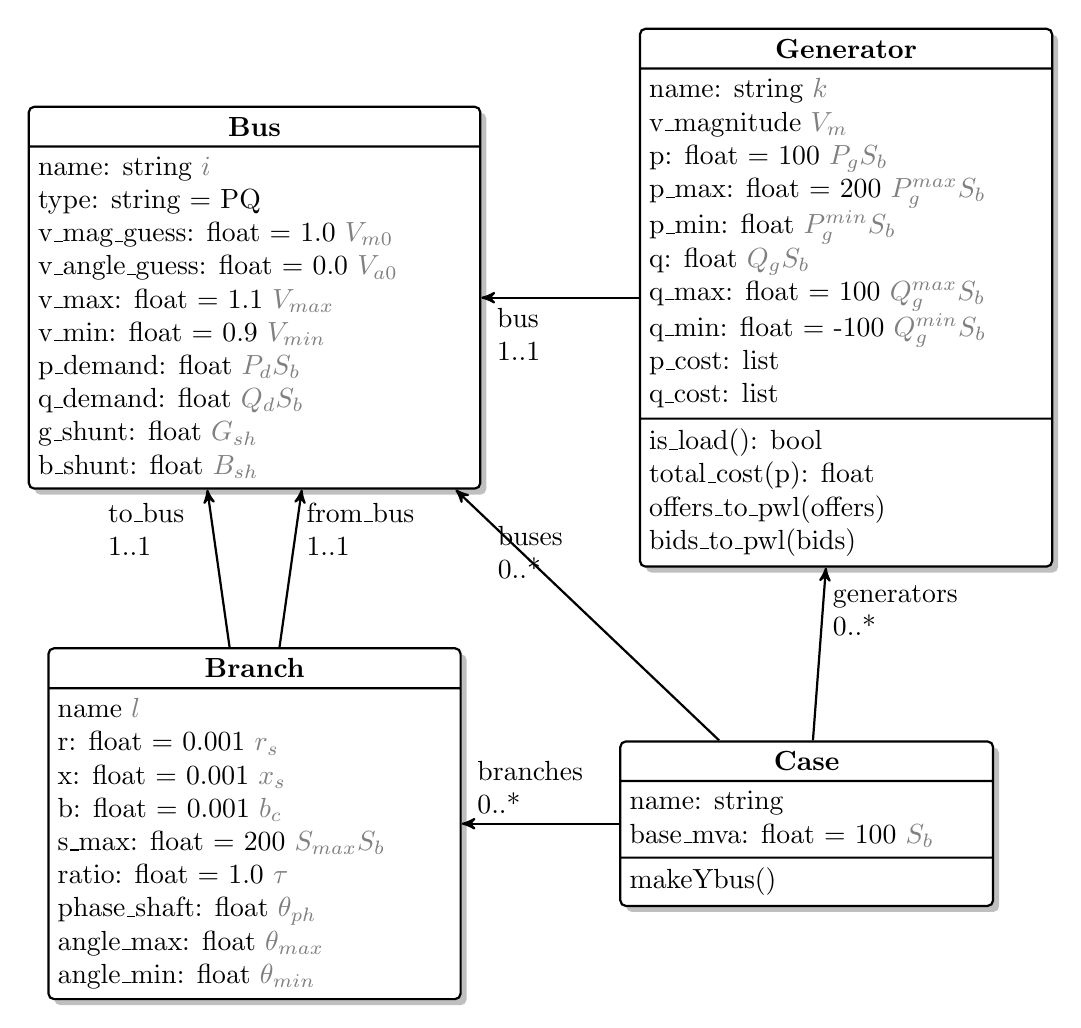
\begin{tikzpicture}[node distance=2cm,thick]

%     \node (Case) [final, rectangle split, rectangle split parts=3]{
%       \textbf{Case}
%       \nodepart[text justified]{second}%
%       name\newline
%       baseMVA\hfill{\color{gray} $S_{base}$}
%       \nodepart[text justified]{third}%
%       makeYbus()\newline
%       makeBdc()\newline
%       dSbus\_dV()\newline
%       dIbr\_dV()\newline
%       dSbr\_dV()\newline
%       dAbr\_dV()\newline
%       d2Sbus\_dV2()\newline
%       d2Ibr\_dV2()\newline
%       d2Sbr\_dV2()\newline
%       d2ASbr\_dV2()\newline
%       d2AIbr\_dV2()
%     };

    \node (Bus) at (0,0) [final, rectangle split, rectangle split parts=2,
            text width=5.5cm]{
      \textbf{Bus}
        \nodepart[text justified]{second}%
        name: string~{\color{gray} $i$}\newline
        type: string = PQ\newline
        v\_mag\_guess: float = 1.0~{\color{gray} $V_{m0}$}\newline
        v\_angle\_guess: float = 0.0~{\color{gray} $V_{a0}$}\newline
        v\_max: float = 1.1~{\color{gray} $V_{max}$}\newline
        v\_min: float = 0.9~{\color{gray} $V_{min}$}\newline
        p\_demand: float~{\color{gray} $P_d S_{b}$}\newline
        q\_demand: float~{\color{gray} $Q_d S_{b}$}\newline
        g\_shunt: float~{\color{gray} $G_{sh}$}\newline
        b\_shunt: float~{\color{gray} $B_{sh}$}};

    \node (Branch) [final, rectangle split, rectangle split parts=2,
    				text width=5cm, below=of Bus]{
      \textbf{Branch}
        \nodepart[text justified]{second}%
        name~{\color{gray} $l$}\newline
%        online: bool = true\newline
        r: float = 0.001~{\color{gray} $r_s$}\newline
        x: float = 0.001~{\color{gray} $x_s$}\newline
        b: float = 0.001~{\color{gray} $b_c$}\newline
        s\_max: float = 200~{\color{gray} $S_{max} S_{b}$}\newline
        ratio: float = 1.0~{\color{gray} $\tau$}\newline
        phase\_shaft: float~{\color{gray} $\theta_{ph}$}\newline
        angle\_max: float~{\color{gray} $\theta_{max}$}\newline
        angle\_min: float~{\color{gray} $\theta_{min}$}}

    edge [->] node[near end,left,text width=12mm]
    {to\_bus 1..1} ([xshift=-6mm]Bus.south)
    edge [->] node[near end,right,text width=16mm]
    {from\_bus 1..1} ([xshift=6mm]Bus.south);

    \node (Gen) [final, rectangle split, rectangle split parts=3,
    		     text width=5cm, right=of Bus]{
      \textbf{Generator}
        \nodepart[text justified]{second}%
        name: string~{\color{gray} $k$}\newline
%        online\newline
        v\_magnitude~{\color{gray} $V_m$}\newline
        p: float = 100~{\color{gray} $P_g S_{b}$}\newline
        p\_max: float = 200~{\color{gray} $P_g^{max} S_{b}$}\newline
        p\_min: float~{\color{gray} $P_g^{min} S_{b}$}\newline
        q: float~{\color{gray} $Q_g S_{b}$}\newline
        q\_max: float = 100~{\color{gray} $Q_g^{max} S_{b}$}\newline
        q\_min: float = -100~{\color{gray} $Q_g^{min} S_{b}$}\newline
        p\_cost: list\newline
        q\_cost: list
        \nodepart[text justified]{third}
        is\_load(): bool\newline
        total\_cost(p): float\newline
        offers\_to\_pwl(offers)\newline
        bids\_to\_pwl(bids)}

    edge [->] node[near end,below,text width=6mm] {bus 1..1} (Bus);

    \node (Case) [final, rectangle split, rectangle split parts=3,
    		      text width=4.5cm, right=of Branch] {
      \textbf{Case}
        \nodepart[text justified]{second}%
        name: string\newline
        base\_mva: float = 100~{\color{gray} $S_{b}$}
		\nodepart[text justified]{third}%
		makeYbus()
    }

    edge [->] node[near end,text width=6mm] {buses 0..*} (Bus)
    edge [->] node[near end,above,text width=6mm] {branches 0..*} (Branch)
    edge [->] node[near end,right,text width=6mm] {generators 0..*} (Gen);

  \end{tikzpicture}
  \caption{Class diagram for the power system model.}
  \label{fig:cls_pylon}
\end{figure}
}{}

As in \textsc{Matpower}, generator active power, and optionally reactive power,
output costs may be defined by convex $n$-segment piecewise linear cost
functions
\begin{equation}
c^{(i)}(p) = m_ip + b_i
\end{equation}
where $p$ is the generator set-point for $p_i \leq p \leq p_{i+1}$ with
$i = 1,2,\dotsc n$, $m_i$ is the variable cost for segment $i$ in
\$/MWh where $m_{i+1} \geq m_i$ and $p_{i+1} > p_i$, and $b_i$ is the
$y$-intercept in \$, also for segment $i$.

Since these cost functions are non-differentiable, the constrained cost variable
approach from \citeA{zimmerman:ccv} is used to make the optimisation problem
smooth.  For each generator $j$ a helper cost variable $y_j$ is added to the
vector of optimisation variables.  Figure~\ref{fig:ccv_function}
\cite[Figure5-3]{pserc:mp_manual} illustrates how the additional inequality
constraints
\begin{equation}
y_j \geq m_{j,i}(p-p_i) + c_i, \quad i = 1\dotsc n
\end{equation}
ensure that $y_j$ lies on or above $c^{(i)}(p)$ as the objective function
minimises the sum of cost variables for all generators:
\begin{equation}
\min_{\theta, V_m, P_g, Q_g, y} \sum_{j=1}^{n_g}y_j
\end{equation}

The extended optimal power flow formulations from \textsc{Matpower} with
user-defined cost functions and generator P-Q capability curves are not used,
but could be applied in further development of this work.

% \section{DC OPF Formulation}
% Piecewise linear cost functions are also used to define generator active power
% costs in the DC optimal power flow formulation.  Since the power flow equations
% are linearised, following the assumptions in equations (\ref{eq:lossless}),
% (\ref{eq:oneperunit}) and (\ref{eq:busangdiff}), the optimal power flow
% problem simplifies to a linear program.  The voltage magnitude variables $V_m$
% and generator reactive power set-point variable $Q_g$ are eliminated following
% the assumption in equation (\ref{eq:busangdiff}) since branch reactive power
% flows depend on bus voltage angle differences.  The objective function reduces to
% \begin{equation}
% \min_{\theta, P_g, y} \sum_{i=1}^{n_g}y_i
% \end{equation}
% Combining the nodal real power injections, expressed as a function of $\Theta$,
% from equation (\ref{eq:bbus}), with active power generation $P_g$ and active
% demand $P_d$, the power balance constraint is
% \begin{equation}
% B_{bus}\Theta + P_{bus,ph} + P_d - C_gP_g = 0
% \end{equation}
% Limits on branch active power flows $B_f\Theta$ and $B_t\Theta$ are enforced by
% the inequality constraints
% \begin{eqnarray}
% B_f\Theta + P_{f,ph} - F_{max}& \leq& 0\\
% -B_f\Theta + P_{f,ph} - F_{max}& \leq& 0
% \end{eqnarray}
% The reference bus voltage angle equality constraint from
% equation (\ref{eq:refbusang}) and the $p_g$ limit constraint from
% (\ref{eq:pglim}) are also applied.

\subsection{Unit De-commitment}
\label{sec:decommit}
The optimal power flow formulations constrain generator set-points between
upper and lower power limits.  The output of expensive generators can be
reduced to the lower limit, but they can not be completely shutdown.  The
online status of generators could be added to the vector of
optimisation variables, but being Boolean the problems would be
mixed-integer non-linear programs which are typically very difficult to
solve.

To compute a least cost commitment and dispatch the unit de-commitment
algorithm from \citeA[p.57]{pserc:mp_manual} is used.  The algorithm
involves shutting down the most expensive units until the
minimum generation capacity is less than the total load capacity and then
solving repeated optimal power flow problems with candidate generating units,
that are at their minimum active power limit, deactivated.  The lowest cost
solution is returned when no further improvement can be made and no candidate
generators remain.

% \begin{algorithm}%[H]
% \caption{Unit de-commitment}
% \label{alg:ud}
% \begin{algorithmic}[1]
% %\STATE $\text{initialise}~N \leftarrow 0$
% %\STATE $P_{d} \leftarrow \text{total load capacity}$
% %\STATE $P_{g}^{min} \leftarrow \text{total min.\ gen.\ capacity}$
% \WHILE{$\sum P_{g}^{min} > \sum P_{d}$}
% %	\STATE $N \leftarrow N + 1$
% 	\STATE shutdown most expensive unit
% \ENDWHILE
%
% %\STATE $\text{solve initial OPF}$
% \STATE $f \leftarrow \text{initial total system cost}$
%
% \REPEAT
% 	\STATE $c \leftarrow \text{generators at } P_{min}$
% 	\FOR{$g$ in $c$}
% 		\STATE $d \leftarrow \text{true}$
% 		\STATE shutdown $g$
% 		\STATE $f^\prime \leftarrow \text{new total system cost}$
% 		\IF{$f^\prime < f$}
% 			\STATE $f \leftarrow f^\prime$
% 			\STATE $g_{c} \leftarrow g$
% 			\STATE $d \leftarrow \text{false}$
% 		\ENDIF
% 		\STATE startup $g$
% 	\ENDFOR
% 	\STATE shutdown $g_c$
% \UNTIL{$d = \text{true}$}
% \end{algorithmic}
% \end{algorithm}

%\newpage
\section{Multi-Agent System}
\label{sec:mas}
Market participants are modelled using PyBrain software agents that use
reinforcement learning algorithms to adjust their behaviour
\cite{schaul:2010}. Their interaction with the market is coordinated in multi-agent simulations,
the structure of which is derived from PyBrain's single player design.

% In PyBrain, agents do not interact directly with their environment, but are
% associated with a particular \textit{task}.
This section describes: discrete and continuous market \textit{environments},
agent \textit{tasks} and \textit{modules} used for policy function
approximation and storing state-action values or action propensities.  The
process by which each agent's policy is updated by a \textit{learner} is
explained and the sequence of interactions between multiple agents and the
market is described and diagrammed.

\subsection{Market Environment}
Each agent has a portfolio of $n_g$ generators associated their environment.
Figure \ref{fig:cls_pyreto} illustrates the association and how the environment
references an instance of the auction market for offer submission.  Each
environment is responsible for \begin{inparaenum}[(i)] \item returning a
vector representation of its current state and \item accepting an action
vector which transforms the environment into a new state. \end{inparaenum}  To
facilitate testing of value function based and policy gradient learning
methods, both discrete and continuous representations of an electric power
trading environment are defined.

\ifthenelse{\boolean{includefigures}}{\begin{figure}
  \label{fig:cls_pyreto}
  \centering
  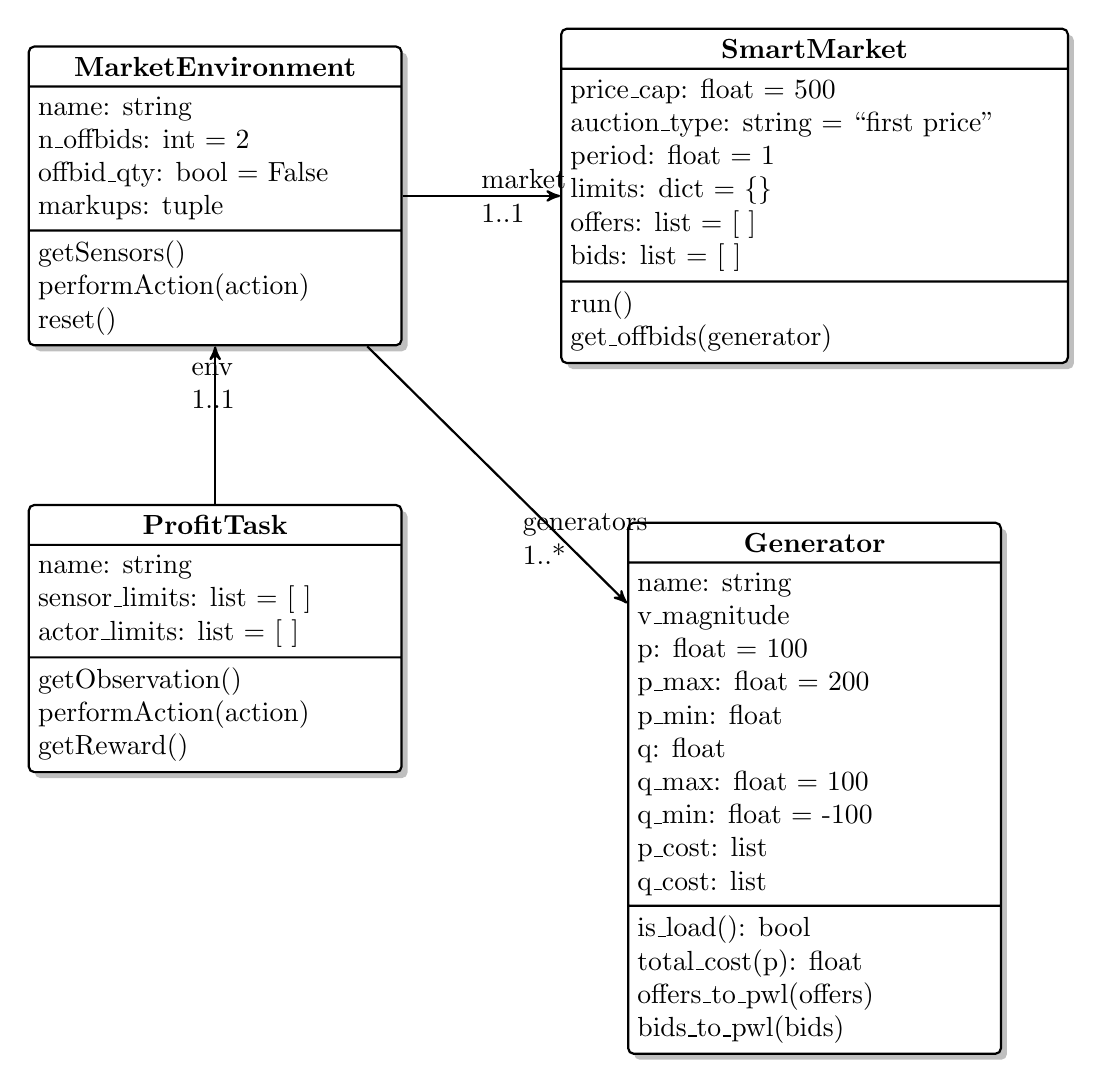
\begin{tikzpicture}[node distance=2cm,thick]

    \node (Mkt) [final, rectangle split, rectangle split parts=3,
    		      		 text width=6.2cm] {
      \textbf{SmartMarket}
        \nodepart[text justified]{second}%
        price\_cap: float = 500\newline
        auction\_type: string = ``first price"\newline
        period: float = 1\newline
        limits: dict = $\lbrace \rbrace$\newline
        offers: list = [ ]\newline
        bids: list = [ ]
		\nodepart[text justified]{third}%
		run()\newline
		get\_offbids(generator)
    };

    \node (Gen) [final, rectangle split, rectangle split parts=3,
    		     text width=4.5cm, below=of Mkt]{
      \textbf{Generator}
        \nodepart[text justified]{second}%
        name: string\newline
%        online\newline
        v\_magnitude\newline
        p: float = 100\newline
        p\_max: float = 200\newline
        p\_min: float\newline
        q: float\newline
        q\_max: float = 100\newline
        q\_min: float = -100\newline
        p\_cost: list\newline
        q\_cost: list
        \nodepart[text justified]{third}
        is\_load(): bool\newline
        total\_cost(p): float\newline
        offers\_to\_pwl(offers)\newline
        bids\_to\_pwl(bids)};

    \node (Env) [final, rectangle split, rectangle split parts=3,
    		      		 text width=4.5cm,left=of Mkt] {
      \textbf{MarketEnvironment}
        \nodepart[text justified]{second}%
        name: string\newline
        n\_offbids: int = 2\newline
        offbid\_qty: bool = False\newline
        markups: tuple
		\nodepart[text justified]{third}%
		getSensors()\newline
		performAction(action)\newline
		reset()
    }

    edge [->] node[near end,text width=10mm] {market 1..1} (Mkt)
    edge [->] node[near end,text width=10mm] {generators 1..*} (Gen);

    \node (Task) [final, rectangle split, rectangle split parts=3,
    		      		 text width=4.5cm,below=of Env] {
      \textbf{ProfitTask}
        \nodepart[text justified]{second}%
        name: string\newline
        sensor\_limits: list = [ ]\newline
        actor\_limits: list = [ ]
		\nodepart[text justified]{third}%
		getObservation()\newline
		performAction(action)\newline
		getReward()
    }

    edge [->] node[near end,text width=6mm] {env 1..1} (Env);

  \end{tikzpicture}
  \caption{Class diagram for the Pyreto.}
\end{figure}
}{}

\subsubsection{Discrete Market Environment}
An environment with $n_s$ discrete states and $n_a$ discrete action
possibilities is defined for agents operating learning methods that make use of
look-up tables. The environment produces a state $s$, where $s \in \mathbb{Z}^+$
and $0\leq s < n_s$, at each simulation step and accepts an action $a$, where $a
\in \mathbb{Z}^+$ and $0\leq a < n_a$.

To keep the size of the state space reasonable, discrete states are derived only
from the total system demand $d=\sum P_d$ where $P_d$ is the vector of active
power demand at each bus.  Informally, the state space is $n_s$ states between the minimum and maximum
demand and the current state for the environment is the index of the state to
which the current demand relates.  Each simulation episode of $n_t$ steps has a
demand profile vector $U$ of length $n_t$, where each element $0 \leq u_i \leq 1$. The
load at each bus $P_{dt} = u_tP_{d0}$ in simulation period $t$, where $P_{d0}$
is the initial demand vector.  The state
size $d_s = d(\max U - \min U)/n_s$ and the state space vector is $\mathscr{S}=d_si$ for
 $i=1\dotsc n_s$. At simulation step $t$, the state returned by the environment
 $s_t = i$ if
$\mathscr{S}_i \leq P_{dt} \leq \mathscr{S}_{i+1}$ for $i = 0\dotsc n_s$.


The action space for a discrete environment is defined by a vector $m$, where
$0 \leq m_i \leq 100$, of percentage markups on marginal cost with length
$n_m$, a vector $w$, where $0 \leq w_i \leq 100$, of percentage capacity
withholds with length $n_w$ and a scalar number of offers $n_o$, where $n_o \in
\mathbb{Z}^+$, to be submitted for each generator associated with the
environment.

A $n_a \times 2n_gn_o$ matrix with all permutations of markup and withhold for
each offer that is to be submitted for each generator is computed. As an
example, Table \ref{tbl:example_actions} shows all possible actions when markups
are restricted to 0, 10\% or 20\%, $m=\lbrace 0,10,20,30 \rbrace$, and 0\% of
capacity may be withheld, $w=\lbrace 0 \rbrace$, from two generators, $n_g=2$,
with one offer submitted for each, $n_o=1$.  Each row corresponds to an action and the column values specify the percentage price
markup and the percentage of capacity to be withheld for each of the $n_gn_o$
offers.  The size of the permutation matrix grows rapidly as $n_o$, $n_g$, $n_m$
and $n_w$ increase.

% For operation with learning methods that use look-up tables to store
% state-action values, an environment with $n_s$ discrete states and $n_a$
% discrete actions is defined.  An agent can not observe offers/bids submitted
% by competitor agents, but may sense other aspects of the power system
% model.  To ensure that the size of the environment state space is
% kept reasonable, the agent is limited to observing a demand forecast.  The
% initial demand at each bus $P_{d0}$, as defined in the original power system
% model, is assumed to be peak and the demand can follow a profile at each
% step $t$ of the simulation (See Chapter \ref{ch:exploitation}).  The state
% space is divided into discrete steps of size $P_{step} = (P_{d0} - P_d^{min}) /
% n_s$, where $P_d^{min}$ is the total demand at the lowest point of the profile.  The
% environment computes the total system demand $P_{dt}$ at step $t$ and returns
% an integer representation of the state
% \begin{equation}
% s_t = \frac{(P_{dt} - P_d^{min})}{P_{step}} + 1.
% \end{equation}
%
% To define the action space, a vector of percentage markups on marginal cost
% $m_e$ is defined for each environment $e$ along with a variable $n_o \in
% \mathbb{Z}^+$ which denotes the number of offers/bids to be submitted by the
% agent.  (A similar vector of percentage markdowns on total capacity has also
% been implemented, but is not used in this thesis.)  A set of all unique
% permutations of markup for $n_o$ offers/bids of length $n_a$ is formed, from
% which the agent must select select.  The action vector that the discrete
% environment is passed consists of a single integer value, corresponding to the
% column index in the agent's action value table.  The quantity and price for
% each offer/bid submitted to the market is taken from the vector of
% permutations using the $a_t$ as the index.  An example of the possible
% permutations of 0, 10 and 20\% markups for a portfolio of two generators is
% given in Table \ref{tbl:example_actions}.  It should be clear how quickly the
% number of possible actions can grow as the number of possible markups and the
% size of the portfolio increases.

\begin{table}
\caption{Example discrete action domain.}
\label{tbl:example_actions}
\begin{center}
\begin{tabular}{c|c|c|c|c}
\hline
$a$ &$m_1$ &$w_1$ &$m_2$ &$w_2$ \\
\hline
 0 &0 &0 &0 &0 \\
 1 &0 &0 &10 &0 \\
 2 &0 &0 &20 &0 \\
 3 &10 &0 &0 &0 \\
 4 &10 &0 &10 &0 \\
 5 &10 &0 &20 &0 \\
 6 &20 &0 &0 &0 \\
 7 &20 &0 &10 &0 \\
 8 &20 &0 &20 &0 \\
\hline
\end{tabular}
\end{center}
\end{table}

\subsubsection{Continuous Market Environment}
% For a power system with $n_b$ buses and $n_l$ branches, the visible state of
% the environment is a vector $s_e$ of length $n_s = 2n_b + 2n_l$.
%$s^i_g$ represents the  for the agent associated with generator $i$.
% $s^i_e$ is composed of sensor values for all buses, branches and generators.
% \begin{equation}
% s^i_{e,l} =
% \begin{bmatrix}
% P_f\\
% Q_f\\
% P_t\\
% Q_t\\
% \mu_{S_f}\\
% \mu_{S_t}
% \end{bmatrix}, \quad
% s^i_{e,b} =
% \begin{bmatrix}
% V_m\\
% V_a\\
% \lambda_P\\
% \lambda_Q\\
% \mu_{v_{min}}\\
% \mu_{v_{max}}
% \end{bmatrix}, \quad
% s^i_{e,g} =
% \begin{bmatrix}
% P_g\\
% \mu_{p_{min}}\\
% \mu_{p_{max}}\\
% \mu_{q_{min}}\\
% \mu_{q_{max}}
% \end{bmatrix}\ \quad
% s^i_e =
% \begin{bmatrix}
% s^i_{e,b}\\
% s^i_{e,b}\\
% s^i_{e,g}
% \end{bmatrix}
% \end{equation}
% Not all of the values are used by each agent and they are filtered according
% to the agent's task.

% For agents operating policy gradient methods, continuous environments that
% output $n_s$ sensors and accept $n_a$ actions are defined.  Each environment
% may be configured for actions that specify just price or price and quantity.  If
% $q_e^i = 0$ where $q_e^i \in (0,1)$ then the agent's action is price selection
% and the offer/bid quantity is determined by the maximum rated capacity of the
% generator in question divided by the number of offers being submitted for it.
% The environment accepts an action vector $a_e$ of length $n_a$ if $q_e^i = 0$,
% otherwise of length $2n_a$.  If $q_e^i = 0$, the $i$-th element of $a_e$ is
% the offered/bid price in \$/MWh, where $i = 1,2,\dotsc n_{in}$.  If $q_e^i =
% 1$, the $i$-th element of $a_e$ is the offered/bid price in \$/MWh, where $i =
% 1,3,5,\dotsc n_{in}-1$ and the $j$-th element of $a_e$ is the offered/bid
% quantity in MW where $j = 2,4,6,\dotsc n_{in}$.  The action vector passed to
% the environment is converted into sets of offers/bids that are submitted to
% the market model.
% %If $q_e^i = 0$, then $qty = p_{max}/n_{in}$.

A continuous market environment that outputs a state vector $s$, where $s_i
\in \mathbb{R}$, and accepts an action vector $a$, where $a_i \in \mathbb{R}$,
is defined for agents operating policy gradient methods.  Scalar variables $m_{u}$ and $w_{u}$ define the upper limit on the percentage
markups on marginal cost and the upper limit on the percentage of capacity that
can be withheld, respectively.  Again, $n_o$ defines the number of offers to be
submitted for each generator associated with the environment.

The state vector can be any set of variables from the power system or market
model.  For example: bus voltages, branch power flows, generator limit
Lagrangian multipliers etc.  Each element of the vector provides one input to the neural network used for policy function approximation.

The action vector $a$ has length $2n_gn_o$.  Element $a_i$, where $0\leq a_i
\leq m_{u}$, corresponds to the percentage price markup and each element
$a_{i+1}$, where $0\leq a_{i+1} \leq w_{u}$, to the percentage of capacity
to be withheld for the $(i/2)^{th}$ offer, where $i=0,2,4,\dotsc,2n_gn_o$.

Not having to discretize the state space and compute a matrix of action
permutations greatly simplifies the implementation of a continuous environment
and increases in $n_g$ and $n_o$ only impact the number of output nodes
on the neural network.

\subsection{Agent Task}
To allow alternative goals (such a profit maximisation or the meeting some
target level for plant utilisation) to be associated with a single type of
environment, an agent does not interact \textit{directly} with its environment,
but is paired with a particular \textit{task}. A task defines the reward
returned to the agent and thus defines the agent's purpose.

For all simulations in this thesis the goal of each agent is to maximise direct
financial profit.  Rewards are defined as the sum of earnings from the previous
period $t$ as determined by the difference between the revenue from cleared
offers and the generator marginal cost at its total cleared quantity.  Using
some measure of risk adjusted return (as in \cite{moody:direct}) might be of
interest in the context of simulated electricity trade and this would simply
involve the definition of a new task and would not require any modification of
the environment.

% Sensor data from the environment is filtered according to the task
% being performed.  Agents with value-function learning methods use a table to
% store state-action values, with one row per environment state.  Thus, observations
% consist of a single value $s_v$, where $s_v \leq n_s$ and $s_v \in
% \mathbb{Z}^+$.

Agents with policy-gradient learning methods approximate their policy functions
using artificial neural networks that are presented with an input vector $s_n$
of length $n_s$ where $s_{n,i} \in \mathbb{R}$.  To condition the environment
state before input to the connectionist system, where possible, a vector $s_{l}$
of lower sensor limts and a vector $s_{u}$ of upper sensor limits is
defined.  These are used to calculated a normalised state vector
\begin{equation}
v = 2\left(\frac{s - s_{l}}{s_{u} - s_{l}}\right) - 1
\end{equation}
where $-1 \leq s_{n,i} \leq 1$.

The output from the policy function approximator $y$ is denormalized using
vectors of minimum and maximum action limits, $a_{min}$ and $a_{max}$
respectively, to give an action vector
\begin{equation}
a = \left(\frac{y + 1}{2}\right)(a_{u} - a_{l}) + a_{l}
\end{equation}
where $0\leq a_i \leq m_{u}$ and $0\leq a_{i+1} \leq w_{u}$ for $i=0,2,4,
\dotsc, 2n_gn_o$.

\subsection{Market Participant Agent}
Each agent is defined as an entity capable of producing an action $a$
based on a previous observation $s$ of its environment.
% , where $a_i$ and $s_i$
% are vectors of length $n_a$ and $n_s$ respectively, where
% $n_s$ is the total number of states and $n_a$ is the total number of actions.
%Figure X shows in UML that
The UML class diagram in Figure \ref{fig:cls_agent} illustrates how each agent
in PyBrain is associated with a \textit{module}, a \textit{learner} (modified
Roth-Erev in the diagram), a \textit{dataset} and an
\textit{explorer}.

\ifthenelse{\boolean{includefigures}}{\begin{figure}
  \centering
  \begin{small}
  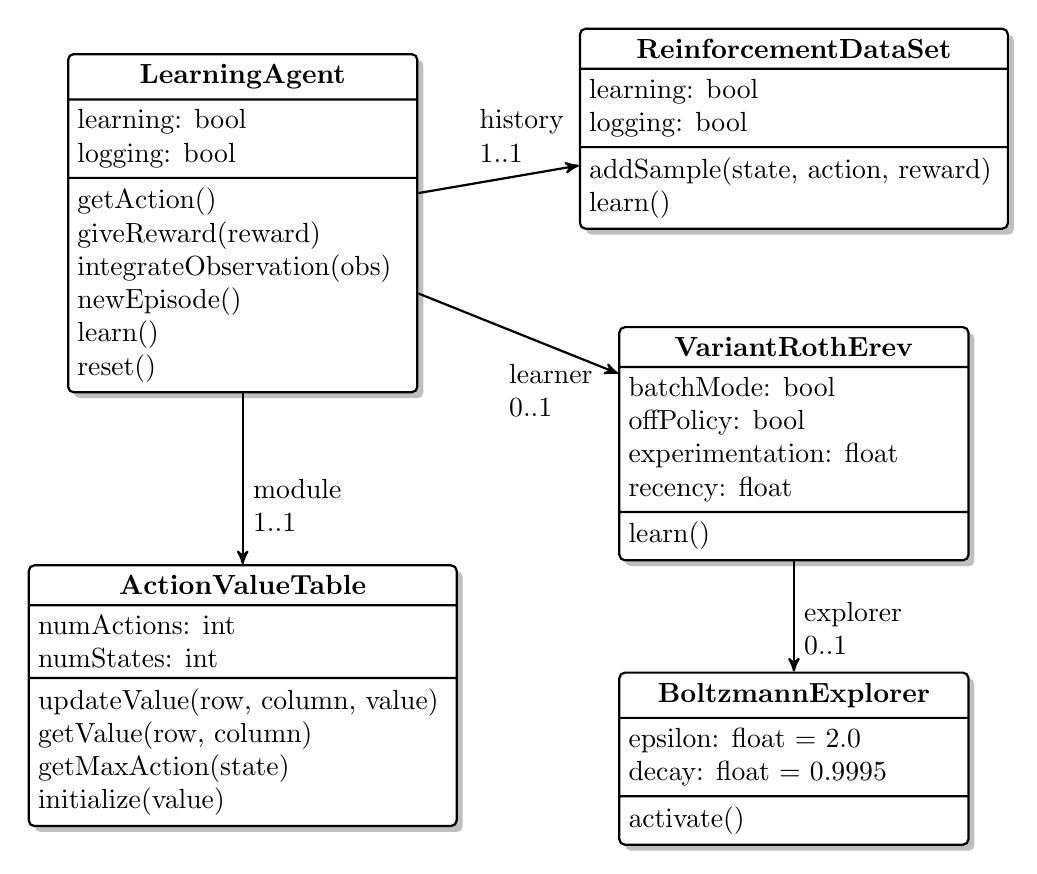
\begin{tikzpicture}[thick]

  \tikzstyle{final}=[rectangle, draw, fill=white, text=black, drop shadow,
    text width=3cm, text centered, rounded corners=2pt]

    \node (Agt) [final, rectangle split, rectangle split parts=3,
    		      		 text width=4.2cm] {
      \textbf{LearningAgent}
        \nodepart[text justified]{second}%
        learning: bool\newline
        logging: bool
		\nodepart[text justified]{third}%
		getAction()\newline
		giveReward(reward)\newline
		integrateObservation(obs)\newline
		newEpisode()\newline
		learn()\newline
		reset()
    };

%    \node (AuxNode01) [text width=4mm,text height=1cm,below of= Agt] {};


    \node (Mod) [final, rectangle split, rectangle split parts=3,
    		     text width=5.2cm,below of=Agt,node distance=6cm] {
      \textbf{ActionValueTable}
        \nodepart[text justified]{second}%
        numActions: int\newline
        numStates: int
		\nodepart[text justified]{third}%
		updateValue(row, column, value)\newline
		getValue(row, column)\newline
		getMaxAction(state)\newline
		initialize(value)
    }
    edge [<-] node[near start,right,text width=15mm,yshift=2mm] {module 1..1}
    (Agt);


    \node (Lrn) [final, rectangle split, rectangle split parts=3,
    		     text width=4.2cm] at (7,-2.8) {
      \textbf{VariantRothErev}
        \nodepart[text justified]{second}%
        batchMode: bool\newline
        offPolicy: bool\newline
        experimentation: float\newline
        recency: float
		\nodepart[text justified]{third}%
		learn()
    }
    edge [<-] node[near start,below,text width=15mm] {learner 0..1} (Agt);


    \node (Dat) [final, rectangle split, rectangle split parts=3,
    		     text width=5.2cm,above of=Lrn,node distance=4cm] {
      \textbf{ReinforcementDataSet}
        \nodepart[text justified]{second}%
        learning: bool\newline
        logging: bool
		\nodepart[text justified]{third}%
		addSample(state, action, reward)\newline
		learn()
    }
    edge [<-] node[near start,above,text width=15mm] {history 1..1} (Agt);


    \node (Exp) [final, rectangle split, rectangle split parts=3,
    		     text width=4.2cm,below of=Lrn,node distance=4cm] {
      \textbf{BoltzmannExplorer}
        \nodepart[text justified]{second}%
        epsilon: float = 2.0\newline
        decay: float = 0.9995
		\nodepart[text justified]{third}%
		activate()
    }
    edge [<-] node[near start,right,text width=15mm,yshift=2mm] {explorer 0..1}
    (Lrn);

  \end{tikzpicture}
  \end{small}
  \caption{Learning agent UML class diagram.}
  \label{fig:cls_agent}
\end{figure}
}{}

The module is used to determine the agent's policy for action selection and
returns an action vector $a$ when activated with a state vector.  When
using value function based methods the module is a $n_s \times n_a$ table of
the form
\begin{equation}
\bordermatrix[{[]}]{%
 & a_0 & a_1 & & a_{n_a} \cr
s_0 & v_{0,0}& v_{0,1}& \dotsb & v_{0,m} \cr
s_1 & v_{1,0}& \ddots& & \vdots \cr
    & \vdots & & \ddots & \vdots \cr
s_{n_s} & v_{n,0} & \dotsb & \dotsb & v_{n_s,n_a}
}
\end{equation}
where each element $v_{i,j}$ is the value in state $i$ associated with
selecting action $j$.  When using a policy gradient method, the module is a
multi-layer feed-forward artificial neural network that outputs a vector $a$
when presented with observation~$s_n$.

The learner can be any reinforcement learning algorithm that modifies the
values/propensities/parameters of the module to increase expected future
reward. The dataset stores state-action-reward triples for each interaction between the
agent and its environment.  The stored history is used by a learners when
computing updates to the module.

Each learner has an association with an explorer that returns an explorative
action $a_e$ when activated with action $a$ from the module.  Softmax and
$\epsilon$-greedy explorers are implemented for discrete action spaces.  Policy
gradient methods use a module that adds Gaussian noise to $a_m$.  The explorer
has a parameter $\sigma$ that relates to the standard deviation of the normal
distribution.  The actual standard deviation
\begin{equation}
\sigma_e = \begin{cases}
\ln(\sigma + 1) + 1 & \text{if $\sigma \geq 0$}\\
\exp(\sigma) & \text{if $\sigma < 0$}
\end{cases}
\end{equation}
to prevent negative $\sigma$ values from causing an error if automatically
adjusted during back-propagation.

%TODO: PG explorer module.

% For example, the $\epsilon$-greedy explorer
% has a randomness parameter $\epsilon$ and a decay parameter $d$.  When the
% $\epsilon$-greedy explorer is activated, a random number $x_r$ is drawn where
% $0 \leq x_r \leq 1$.  If $x_r < \epsilon$ then a random vector of the same
% length as $a_e$ is returned, otherwise $a_e = a_m$.

\subsection{Simulation Event Sequence}
\ifthenelse{\boolean{includefigures}}{\begin{figure}
  \centering
  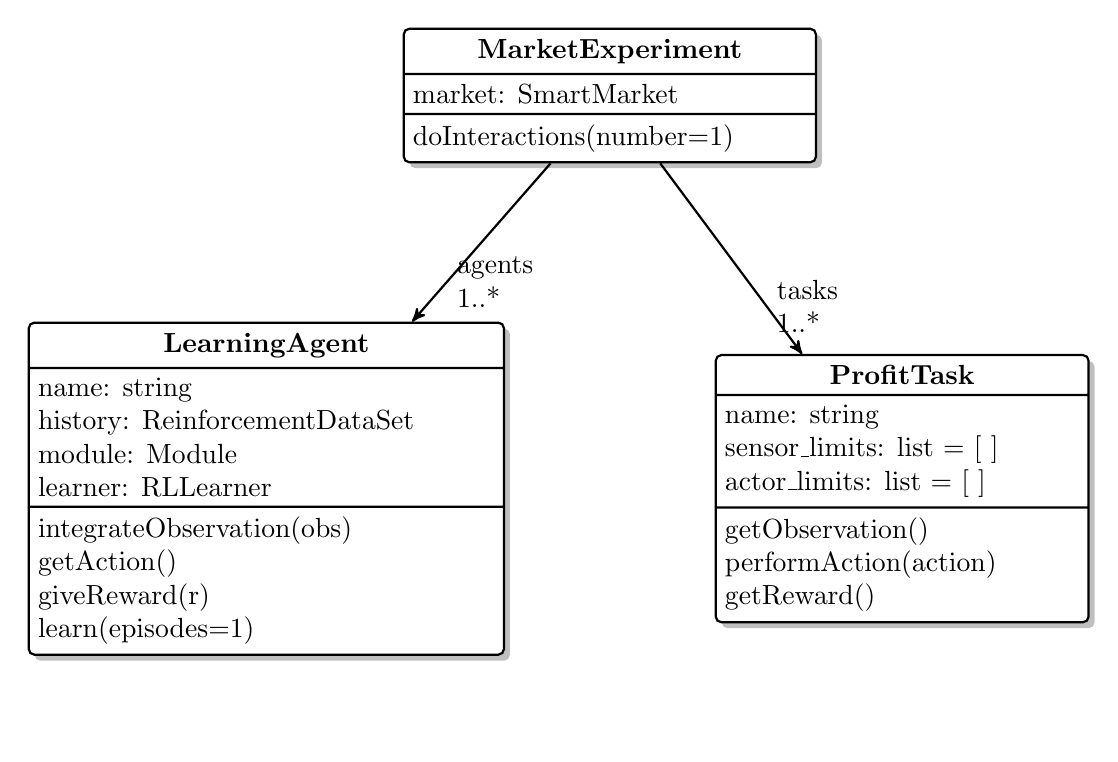
\begin{tikzpicture}[thick]

    \node (Agent) [final, rectangle split, rectangle split parts=3,
    		       text width=5.8cm] {
      \textbf{LearningAgent}
        \nodepart[text justified]{second}%
        name: string\newline
        history: ReinforcementDataSet\newline
        module: Module\newline
        learner: RLLearner
		\nodepart[text justified]{third}%
		integrateObservation(obs)\newline
		getAction()\newline
		giveReward(r)\newline
		learn(episodes=1)
    };

    \node (AuxNode01) [text width=4mm,text height=6cm,right=of Agent] {};


    \node (Task) [final, rectangle split, rectangle split parts=3,
    		      text width=4.5cm,right=of AuxNode01] {
      \textbf{ProfitTask}
        \nodepart[text justified]{second}%
        name: string\newline
        sensor\_limits: list = [ ]\newline
        actor\_limits: list = [ ]
		\nodepart[text justified]{third}%
		getObservation()\newline
		performAction(action)\newline
		getReward()
    };


    \node (Expr) [final, rectangle split, rectangle split parts=3,
    		      text width=5cm,above=of AuxNode01] {
      \textbf{MarketExperiment}
        \nodepart[text justified]{second}%
        market: SmartMarket
		\nodepart[text justified]{third}%
		doInteractions(number=1)
    }
    edge [->] node[near end,right,text width=6mm] {agents 1..*} (Agent)
    edge [->] node[near end,right,text width=6mm] {tasks 1..*} (Task);

  \end{tikzpicture}
  \caption{Class diagram for Pyreto market experiment.}
  \label{fig:cls_experiment}
\end{figure}
}{}
Each simulation consists of one or more task-agent pairs.  Figure
\ref{fig:cls_experiment} shows the class associations for a simulation
experiment.  At the beginning of each simulation step (trading period) $t$ the
market is initialised and all previous offers are removed.  Figure
\ref{fig:seq_action} is a UML sequence diagram that illustrates the process of
choosing and performing an action that follows.  For each task-agent tuple an
observation $s_t$ is retrieved from the task and integrated into the agent.  When an action
is requested from the agent its module is activated with $s_t$ and the action
$a_{e,t}$ is returned.  Action $a_{e,t}$ is performed on the environment
associated with the agent's task.

\ifthenelse{\boolean{includefigures}}{\begin{figure}
  \centering
  \begin{small}
  \begin{sequencediagram}
    \newthread{exp}{:Experiment}
    \newinst{tsk}{:Task}
    \newinst{env}{:Environment}
    \newinst{agt}{:Agent}
    \newinst{mod}{:Module}
    \newinst{epl}{Explorer}

    \begin{call}{exp}{getObservation()}{tsk}{$s_t$}
      \begin{call}{tsk}{getSensors()}{env}{$s_e$}
      \end{call}
      \begin{callself}{tsk}{normalise($s_e$)}{$s_t$}
      \end{callself}
    \end{call}

    \begin{call}{exp}{integrateObservation($s_t$)}{agt}{}
      \begin{callself}{agt}{setLastObs($s_t$)}{}
      \end{callself}
    \end{call}

    \begin{call}{exp}{getAction()}{agt}{$a_e$}
      \begin{callself}{agt}{getLastObs()}{$s_t$}
      \end{callself}
      \begin{call}{agt}{activate($s_t$)}{mod}{$a$}
      \end{call}
      \begin{call}{agt}{activate($a$)}{epl}{$a_e$}
      \end{call}
      \begin{callself}{agt}{setLastAction()}{$a_e$}
      \end{callself}
    \end{call}

    \begin{call}{exp}{performAction($a_e$)}{tsk}{}
      \begin{callself}{tsk}{denormalise($a_e$)}{$a_t$}
      \end{callself}
      \begin{call}{tsk}{performAction($a_t$)}{env}{}
      \end{call}
    \end{call}

  \end{sequencediagram}
  \end{small}
  \caption{Action selection sequence diagram.}
  \label{fig:seq_action}
\end{figure}
}{}
\ifthenelse{\boolean{includefigures}}{\begin{figure}
  \centering
  \begin{small}
  \begin{sequencediagram}
    \newthread{exp}{:Experiment}
    \newinst{tsk}{:Task}
    \newinst{env}{:Environment}
    \newinst{agt}{:Agent}
    \newinst{mkt}{:Market}
    \newinst{dat}{:Dataset}

    \begin{call}{exp}{getReward()}{tsk}{$r_t$}
      \begin{call}{tsk}{getGenerators()}{env}{$g$}
      \end{call}
      \begin{call}{tsk}{getClearedOffers($g$)}{mkt}{$\sigma_g$}
      \end{call}
      \begin{callself}{tsk}{getEarnings($\sigma_g$)}{$r_t$}
      \end{callself}
    \end{call}

    \begin{call}{exp}{giveReward($r_t$)}{agt}{}
      \begin{callself}{agt}{getLastObs()}{$s_t$}
      \end{callself}
      \begin{callself}{agt}{getLastObs()}{$a_e$}
      \end{callself}
      \begin{call}{agt}{addSample($s_t$,$a_e$,$r_t$)}{dat}{}
      \end{call}
    \end{call}

  \end{sequencediagram}
  \end{small}
  \caption{Sequence diagram for the reward process.}
  \label{fig:seq_reward}
\end{figure}
}{}

When all actions have been performed the offers are cleared by the market using
the solution to a newly formed optimal power flow problem.  Figure
\ref{fig:seq_reward} illustrates the subsequent reward process.  The cleared
offers associated with the generators in the task's environment are retrieved from the market and the
reward $r_t$ is computed from the difference between revenue and marginal
cost at the total cleared quantity.
% For each generator in the agent's portfolio
% that was previously online and is not dispatched, a shutdown cost $c_{down}$ is
% subtracted from the reward.
% \begin{equation} r_t = \mbox{revenue} - (c_{fixed} + c_{variable})
% \end{equation}
The reward $r_t$ is given to the associated agent and the value is stored, along
with the previous state $s_t$ and selected action $a_{e,t}$, under a new sample
is the dataset.

\ifthenelse{\boolean{includefigures}}{\begin{figure}
  \centering
  \begin{small}
  \begin{sequencediagram}
    \newthread{exp}{:Experiment}
    \newinst[1.5]{agt}{:Agent}
    \newinst{lrn}{:Learner}
    \newinst[1]{dat}{:Dataset}
    \newinst{mod}{:Module}

    \begin{call}{exp}{learnEpisodes($1$)}{agt}{}
      \begin{call}{agt}{learn()}{lrn}{}
        \begin{sdblock}{batchMode}{}
          \begin{call}{lrn}{getSample()}{dat}{$s$, $a$, $r$}
          \end{call}
          \begin{call}{lrn}{getValue($s_{-1}$,$a_{-1}$)}{mod}{$q_v$}
          \end{call}
          \begin{call}{lrn}{getValue($s$,$a$)}{mod}{$q_{+1}$}
          \end{call}
          \begin{callself}{lrn}{getQ($q_v$,$\alpha$,$r$,$\gamma$,$q_{+1}$)}{$q_u$}
          \end{callself}
          \begin{call}{lrn}{updateValue($s_{-1}$,$a_{-1}$,$q_u$)}{mod}{}
          \end{call}
        \end{sdblock}
      \end{call}
    \end{call}

  \end{sequencediagram}
  \end{small}
  \caption{Sequence diagram for the SARSA learning process.}
  \label{fig:seq_learn}
\end{figure}
}{}

The learning process is illustrated by the UML sequence diagram in Figure
\ref{fig:seq_learn}.  Each agent learns from its actions using $r_t$, at which
point the values or parameters of the module associated with the agent are
updated according to the output of the learner's algorithm.  Each agent is then
reset and the history of states, actions and rewards is cleared.

The combination of an action, reward and learning process for each agent
constitutes one step of the simulation and the processes are repeated until a
specified number of steps are complete.

% \subsection{Auction Example}
% To demonstrate the simulation process this example will walk through a single
% step.  The six bus power system model used in this example is adapted from
% \citeA[pp.~104, 112, 119, 123-124, 549]{wood:pgoc} and a one-line diagram for
% the case is given in Figure \ref{fig:case6ww}.  The model has 3 generators
% with a total capacity of 530MW and the total system load is 210MW.  The
% initial generator costs are defined by quadratic functions of the form $a + bx
% + cx^2$, where $x$ is the generator set-point, with the parameters are given in
% Table \ref{tbl:ex_coeffs}.
% \begin{table}
% \begin{center}
% \begin{tabular}{c|c|c|c}
% \hline
% Generator bus & $a$ & $b$ & $c$ \\
% \hline
% 1 & 215.0 & 10.0 & 0.005 \\
% 2 & 200.0 & 12.0 & 0.008 \\
% 3 & 240.0 & 15.0 & 0.010 \\
% \hline
% \end{tabular}
% \end{center}
% \caption{Generator cost function coefficients.}
% \label{tbl:ex_coeffs}
% \end{table}
%
% Suppose each offers half of its capacity with a markup of 10\% and the
% remainder marked up by 20\%.  This correlates to a set of offers with
% quantities and prices given in Table \ref{tbl:ex_offers}.
% \begin{table}
% \begin{center}
% \begin{tabular}{c|cc|cc}
% \hline
% Generator bus & \multicolumn{2}{c}{Offer 1} & \multicolumn{2}{|c}{Offer 2}\\
%  & MW & \$/MWh & MW & \$/MWh \\
% \hline
% 1 & 100 & 20 & 100 & 30 \\
% 2 & 75  & 25 & 75  & 40 \\
% 3 & 90  & 30 & \sout{90}  & \sout{50} \\
% \hline
% \end{tabular}
% \end{center}
% \caption{Offered quantities and prices.}
% \label{tbl:ex_offers}
% \end{table}
% Setting a price
% cap of \$45 causes the second offer from the generator at bus 3 to be withheld
% and ignored in the conversion to piecewise linear cost functions.
%
% Table
% \ref{tbl:ex_pwl} lists the points of the resulting piecewise linear cost
% functions and Figure X plots the original marginal cost function and the cost
% function corresponding to the submitted offers for the generator at bus 1.
% \begin{table}
% \begin{center}
% \begin{tabular}{c|c|c|c}
% \hline
% Generator bus & $(P_g, C)$ & $(P_g, C)$ & $(P_g, C)$ \\
% \hline
% 1 & (0, 215) & (100, 10.0) & (200, 0.005) \\
% 2 & (0, 200) & (75, 12.0) & (150, 0.008) \\
% 3 & (0, 240) & (90, 15.0) & (180, 0.010) \\
% \hline
% \end{tabular}
% \end{center}
% \caption{Piecewise linear cost function points.}
% \label{tbl:ex_pwl}
% \end{table}
% Also plotted is the generator set-point from the optimal power flow
% solution and the elevation of the nodal marginal price caused by network
% congestion and branch losses.  The diagram indicates the difference between the
% original marginal cost function and the cleared price that is the earnings from
% that generator and would be used as part of the reward for the responsible
% agent.

\section{Summary}
The power exchange auction market model defined in this chapter provides a layer
of abstraction over the underlying optimal power flow problem and presents
agents with a simple interface for selling power.  The modular nature of the
simulation framework described allows the type of learning algorithm, policy
function approximator, exploration technique or task to be easily changed.  The
framework can simulate competitive electric power trade using almost any
conventional bus-branch power system model with little configuration, but
provides the facilities for adjusting all of the main aspects of a simulation.
The framework's modularity and support for easy configuration is intended to
allow transparent comparison of learning methods under a wide variety of
different scenarios.


% Critical assessment of own work.
\chapter{Nash Equilibrium Analysis}
\label{ch:learningtotrade}
This chapter examines the convergence to a Nash
equilibrium\footnote{Informally, a Nash equlibrium is a point at which no
player is motivated to deviate from its strategy as it would result in lower
gain.} of agents compteting with portfolios of generating plant.  Value
function based and policy gradient reinforcement learning algorithms are
compared in their ability to converge on an optimal policy using a six bus
electric power system model.

\section{Introduction}
To the best of the author's knowledge, this thesis presents the first case of
policy gradient reinforcement learning methods being applied to electricity
trading problems.  As a first step it is necessary to confirm that when using
these methods, a system of multiple agents will converge to the same Nash
equilibrium that conventional closed-form simulation techniques produce.

This is the same approach by \citeA{krause:nash06} before performing the study
of congestion management techniques that is reviewed in Section
\ref{sec:related_cong}.  Nash equilibria can be difficult
to determine in complex systems so the experiment presented here utilises a
model simple enough that it can be determined through exhaustive search.

By observing the actions taken and the reward received by each agent over the
initial simulation periods it is possible to compare different configurations
of the algorithms in their speed of convergence to an optimal policy.  In the
following sections the objectives of this experiment are explictly defined, the
setup of the simulations is explained and simulation results with discussion
and critical analysis are provided.

\section{Aims and Objectives}
Some elements of this experiment are very similar to those presented in
\citeA{krause:nash06} and the initial aim is to reproduce those results.
The additional objectives are to show that:
\begin{itemize}
  \item Policy gradient methods converge to the same Nash equilibrium as value
  function based methods.
  \item The differences in speed of convergence to an optimal policy between
  the learning methods.
%   \item The sensitivity of policy convergence to algorithm parameter choices
%   and policy function approximation structure.
\end{itemize}
Meeting these objectives aims to provide a basis for more complicated
experiments that are less intuitively tractable.

\section{Method of Simulation}
% Each learning method is tested individually using a range of parameter
% configurations.  A power system model with one bus, one generator $k$ and
% one dispatchable load $l$.  In this
% context, the market clearing process is equivalent to creating offer and bids
% stacks and finding the point of intersection.  A passive agent is associated
% with the dispatchable load.  This agent bids for $-p_{g,l}^{min}$ at marginal
% cost each period regardless of environment state or reward signal.  A
% dispathcable load is used instead of a constant load to allow a price to be
% set. Generator $k$ is given sufficient capacity to supply the demand
% of the dispatchable load, $p_{g,k}^{max} > -p_{g,l}^{min}$, and the marginal of
% the $k$ is half that of the load $l$.  The generator and dispatchable load
% attributes are given in Table X.  A price cap for the market is set to twice the
% marginal cost of the $l$ at full capacity, $p_{g,l}^{min}$.  The DC optimal
% power flow formulation (See Section \ref{sec:opf}, above) is used to clear the
% market and reactive power trade is omitted.
Learning methods are compared in this experiment by repeating the same
simulation with different algorithms used by the agents.  An alternative
might be to use a combination of methods in the same simulation, but the
approach used here is intended to be an extension of the work in
\citeA{krause:nash06}.

Each simulation uses the six bus electric power system model adapted from
\citeA[pp.~104, 112, 119, 123-124, 549]{wood:pgoc}.  The six buses are
connected by eleven transmission lines at 230kV.  It contains three generating
units with a total capacity of 440MW and loads at three locations, each of
70MW. The connectivity of the branches and the locations of the generators and
loads is shown in Figure~\ref{fig:case6ww}.  Data for the power system model is
provided in Appendix \ref{adx:case6ww} and is distributed with the software
developed for this thesis (See Appendix \ref{sec:pylon}).

Two sets of generator operating costs are defined to create two different
equilibria for investigation. The first set is listed in Table
\ref{tbl:case6ww_gencost1}. It defines two low cost generators that can not
offer a price greater than the marginal cost of the most expensive generator
when the maximum markup is applied.  The second set is listed in Table
\ref{tbl:case6ww_gencost2} and narrows the cost differences such that offer
prices overlap and may exceed the marginal cost of the most expensive
generator.

%\begin{figure}
\label{fig:case6ww}
\centering
\begin{scriptsize}
\begin{tikzpicture}[thick]

\coordinate (c1) at (0,4);
\coordinate (c2) at (5,6.5);
\coordinate (c3) at (10,4);
\coordinate (c4) at (0,0);
\coordinate (c5) at (5,-2.5);
\coordinate (c6) at (10,0);
\coordinate (over) at (0,3.75);

\busbar{b1}{c1}{20mm}
\busbar{b2}{c2}{30mm}
\busbar{b3}{c3}{20mm}
\busbar{b4}{c4}{20mm}
\busbar{b5}{c5}{30mm}
\busbar{b6}{c6}{20mm}

% Branch 1-2.
\draw[line] ([xshift=5mm] b1.north) node[rotate=90,above right]{$15.41$}
node[rotate=90,below right]{$-9.58$} -- ++(0,3.75) -| ([xshift=-8mm] b2.north)
node[rotate=90,above right]{$-15.14$} node[rotate=90,below right]{$5.70$};
% Branch 1-4.
\draw[line] ([xshift=-5mm] b1.south) node[rotate=90,above left]{$33.95$}
node[rotate=90,below left]{$22.50$} -- ([xshift=-5mm] b4.north)
node[rotate=90,above right]{$-33.15$} node[rotate=90,below right]{$-23.46$};
% Branch 1-5.
\draw[line] ([xshift=5mm] b1.south) node[rotate=90,above left]{$27.86$}
node[rotate=90,below left]{$12.80$} -- ([xshift=5mm,yshift=-15mm] b1.south)
-- ([xshift=-8mm,yshift=15mm] b5.north) -- ([xshift=-8mm] b5.north)
node[rotate=90,above right]{$-27.11$} node[rotate=90,below right]{$-16.20$};
% Branch 2-3.
\draw[line] ([xshift=8mm] b2.north) node[rotate=90,above right]{$0.29$}
node[rotate=90,below right]{$-11.76$} -- ++(0,1.25) -| ([xshift=-5mm] b3.north)
node[rotate=90,above right]{$-0.25$} node[rotate=90,below right]{$5.18$};
% Branch 2-4.
\draw[line,ultra thick] ([xshift=-8mm] b2.south) node[rotate=90,above
left]{$41.74$} node[rotate=90,below left]{$43.11$} --
([xshift=-8mm,yshift=-15mm] b2.south) -- node[sloped,above]{$\vert S_{max}^5
\vert = 60.0$} ([xshift=5mm,yshift=15mm] b4.north) -- ([xshift=5mm] b4.north)
node[rotate=90,above right]{$-40.06$} node[rotate=90,below right]{$-41.83$};
% Branch 2-5.
\draw[line] (b2.south) node[rotate=90,above left]{$17.35$}
node[rotate=90,below left]{$14.93$} -- (b5.north) node[rotate=90,above
right]{$-16.81$} node[rotate=90,below right]{$-17.46$};
% Branch 2-6.
\draw[line] ([xshift=8mm] b2.south) node[rotate=90,above left]{$25.03$}
node[rotate=90,below left]{$12.67$} -- ([xshift=8mm,yshift=-15mm] b2.south)
-- ([xshift=-5mm,yshift=15mm] b6.north) -- ([xshift=-5mm] b6.north)
node[rotate=90,above right]{$-24.49$} node[rotate=90,below right]{$-16.38$};
% Branch 3-5.
\draw[line] ([xshift=-5mm] b3.south) node[rotate=90,above left]{$23.18$}
node[rotate=90,below left]{$21.57$} -- ([xshift=-5mm,yshift=-15mm] b3.south)
-- ([xshift=8mm,yshift=15mm] b5.north) -- ([xshift=8mm] b5.north)
node[rotate=90,above right]{$-21.99$} node[rotate=90,below right]{$-24.28$};
% Branch 3-6.
\draw[line] ([xshift=5mm] b3.south) node[rotate=90,above left]{$47.50$}
node[rotate=90,below left]{$59.90$} -- ([xshift=5mm] b6.north)
node[rotate=90,above right]{$-46.45$} node[rotate=90,below right]{$-56.82$};
% Branch 4-5.
\draw[line] ([xshift=5mm] b4.south) node[rotate=90,above left]{$3.21$}
node[rotate=90,below left]{$-4.71$} -- ++(0,-3.75) -| ([xshift=-8mm] b5.south)
node[rotate=90,above left]{$-3.19$} node[rotate=90,below left]{$-3.03$};
% Branch 5-6.
\draw[line] ([xshift=8mm] b5.south) node[rotate=90,above left]{$-0.90$}
node[rotate=90,below left]{$-9.03$} -- ++(0,-1.25) -| ([xshift=-5mm] b6.south)
node[rotate=90,above left]{$0.94$} node[rotate=90,below left]{$3.21$};

% Generator 1.
\genset{g1}{$(c1)+(-5mm,15mm)$}
\draw[line] ([xshift=-5mm] b1.north) -- node[sloped,above]{$77.22$}
node[sloped,below]{$25.72$} (g1.south);
% Generator 2.
\genset{g2}{$(c2)+(0,15mm)$}
\draw[line] (b2.north) -- node[sloped,above]{$69.27$}
node[sloped,below]{$64.65$} (g2.south);
% Generator 3.
\genset{g3}{$(c3)+(5mm,15mm)$}
\draw[line] ([xshift=5mm] b3.north) -- node[sloped,above]{$70.42$}
node[sloped,below]{$86.64$} (g3.south);

% Load 1.
\loadd{l1}{$(c4)-(5mm,15mm)$}
\draw[line] (l1.south) -- node[sloped,above]{$70.00$}
node[sloped,below]{$70.00$} ([xshift=-5mm] b4.south);
% Load 2.
\loadd{l2}{$(c5)-(0mm,15mm)$}
\draw[line] (l2.south) -- node[sloped,above]{$70.00$}
node[sloped,below]{$70.00$} (b5.south);
% Load 3.
\loadd{l3}{$(c6)+(5mm,-15mm)$}
\draw[line] (l3.south) -- node[sloped,above]{$70.00$}
node[sloped,below]{$70.00$} ([xshift=5mm] b6.south);

\end{tikzpicture}
\end{scriptsize}
\caption{One line diagram for six bus power system model from [].}
\end{figure}


\begin{table}
\begin{center}
\begin{tabular}{c|c|c|c|c}
\hline
Gen &$C_{down}$ &$a$ &$b$ &$c$ \\
\hline\hline
 1 &100 &0.0 &4.0 &200.0 \\
 2 &100 &0.0 &3.0 &200.0 \\
 3 &100 &0.0 &6.0 &200.0 \\
\hline
\end{tabular}
\caption{Generator cost configuration 1 for 6-bus case.}
\label{tbl:case6ww_gencost1}
\end{center}
\end{table}

\begin{table}
\begin{center}
\begin{tabular}{c|c|c|c|c}
\hline
Gen &$C_{down}$ &$a$ &$b$ &$c$ \\
\hline\hline
 1 &100 &0.0 &5.1 &200.0 \\
 2 &100 &0.0 &4.5 &200.0 \\
 3 &100 &0.0 &6.0 &200.0 \\
\hline
\end{tabular}
\caption{Generator cost configuration 2 for 6-bus case.}
\label{tbl:case6ww_gencost2}
\end{center}
\end{table}

No load profile is defined, the system load is assumed to be peak for all
simulation periods, so only one system state is defined for the value function
based algorithms.  The minimum operating point, $P^{min}$, for all generators
is made to be zero so as to simplify the experiment and avoid the need to
use the unit decommitment algorithm defined in Section \ref{sec:decommit}.

The maximum capacity for the most expensive generator $P^{max}_3$=220MW such
that it may supply almost all of the load if it is dispatched.  This
generator is associated with a passive agent that always offers a maginal
cost.  For the other generators $P^{max}_1$=110MW and $P^{max}_2$=110MW.  These
two generators are each associated with am active learning agent whose activity
in the market is restricted to one offer of maximum capacity in each period,
at a price representing a markup of between 0 and 30\% on marginal cost.
Value function based methods are restricted to discrete markup steps of 10\%,
giving possible markup actions of 0, 10, 20 and 30\%. The market price cap is
set such that it is never reached by any markup and does not complicate the
experiment.  Discrimnatory pricing (pay-as-bid) is used in order to provide a
clearer reward signal to agents with low cost generators.

The learning methods compared are Q-learning, ENAC, REINFORCE and the variant
Roth-Erev technique.  For Q-learning $\alpha=0.3$, $\gamma=0.99$ and
$\epsilon$-greedy action selection is used with $\epsilon=0.9$ and $d=0.97$.
For Roth-Erev learning $\epsilon=0.55$, $\phi=0.3$ and Boltzmann action
selection is used with $\tau=100$ and $d=0.98$.  Both REINFORCE and ENAC use a
three-layer neural network with one linear input node, two hidden $\tanh$
nodes, one output $\tanh$ node and bias nodes in the hidden and output layers.

As in \citeA{krause:nash06}, the point of Nash equilibrium is established by
computing each agent's reward for all possible combinations of markup.  The
rewards for Agent 1 and Agent 2 under cost configuration 1 are given in Table
\ref{tbl:nash1}.  The Nash equilibrium points are marked with a *.  It shows
that the optimal policy for each agent is to apply the maximum markup to each
offer as this never results in thier generators failing to be dispatched. The
rewards under cost configuration 2 are given in Table \ref{tbl:nash2}. It
shows that the optimal point occurs when Agent 2 applies its maximum markup
and Agent 1 offers a price just below the marginal cost of the passive agent's
generator.

\begin{table}
\begin{center}
\begin{small}
\begin{tabular}{c.{2.2}|.{2.1}.{2.1}|.{2.1}.{2.1}|.{2.1}.{2.1}|.{3.1}.{2.1}|}
\cline{3-10}
 & &\multicolumn{8}{c|}{$G_1$} \\
\cline{3-10}
 & &\multicolumn{2}{c|}{0.0\%} &\multicolumn{2}{c|}{10.0\%} &\multicolumn{2}{c|}{20.0\%} &\multicolumn{2}{c|}{30.0\%} \\
 & &r_1 &r_2 &r_1 &r_2 &r_1 &r_2 &r_1 &r_2 \\
\hline
\multicolumn{1}{|c|}{\multirow{4}{*}{$G_2$}} &0.0\% &0.0 &0.0 &40.0 &0.0 &80.0 &0.0 &120.0 &0.0 \\
\multicolumn{1}{|c|}{} &10.0\% &0.0 &33.0 &40.0 &33.0 &80.0 &33.0 &120.0 &33.0 \\
\multicolumn{1}{|c|}{} &20.0\% &0.0 &66.0 &40.0 &66.0 &80.0 &66.0 &120.0 &66.0 \\
\multicolumn{1}{|c|}{} &30.0\% &0.0 &99.0 &40.0 &99.0 &80.0 &99.0 &120.0^*
&99.0^* \\
\hline
\end{tabular}
\caption{Agent rewards under cost configuration~1}
\label{tbl:nash1}
\end{small}
\end{center}
\end{table}

\begin{table}
\begin{center}
\begin{small}
\begin{tabular}{c.{2.2}|.{2.1}.{3.1}|.{2.1}.{3.1}|.{2.1}.{3.1}|.{2.1}.{3.1}|}
\cline{3-10}
 & &\multicolumn{8}{c|}{$G_1$} \\
\cline{3-10}
 & &\multicolumn{2}{c|}{0.0\%} &\multicolumn{2}{c|}{10.0\%} &\multicolumn{2}{c|}{20.0\%} &\multicolumn{2}{c|}{30.0\%} \\
 & &r_1 &r_2 &r_1 &r_2 &r_1 &r_2 &r_1 &r_2 \\
\hline
\multicolumn{1}{|c|}{\multirow{4}{*}{$G_2$}} &0.0\% &0.0 &0.0 &51.0 &0.0 &0.0 &0.0 &0.0 &0.0 \\
\multicolumn{1}{|c|}{} &10.0\% &0.0 &49.5 &51.0 &49.5 &0.0 &49.5 &0.0 &49.5 \\
\multicolumn{1}{|c|}{} &20.0\% &0.0 &92.2 &51.0 &99.0 &0.0 &99.0 &0.0 &99.0 \\
\multicolumn{1}{|c|}{} &30.0\% &0.0 &126.8 &54.8^* &138.4^* &0.0 &148.5 &0.0
&148.5 \\
\hline
\end{tabular}
\caption{Agent rewards under cost configuration~2}
\label{tbl:nash2}
\end{small}
\end{center}
\end{table}

\section{Simulation Results}
Each action taken by an agent and the consequent reward is recorded for each
simulation.  Values are averaged over the 10 simulation runs and standard
deviations calculated using the formula
\begin{equation}
SD = \sum_{i=0}^{N}\frac{(x_i - m)^2}{N-1}
\end{equation}
where $x_i$ is the action or reward value in simulation $i$ of $N$ simulation
runs and $m$ is the mean of the values.

Figure \ref{fig:5_1_action_a1} plots the average markup on marginal cost and
the standard deviation over the 10 simulation runs for Agent 1 under the first
price configuration using the variant Roth-Erev, Q-learning, REINFORCE and ENAC
learning methods.  The second $y$-axis in each plot gives the value of
the exploration parameter for each method.  Figure \ref{fig:5_1_action_a2}
plots the same quantities for Agent 2.  Plots of reward are not given as
generator prices and the market are configured such that an agent's reward is
directly proportional to its action.

\begin{figure}
  \centering
  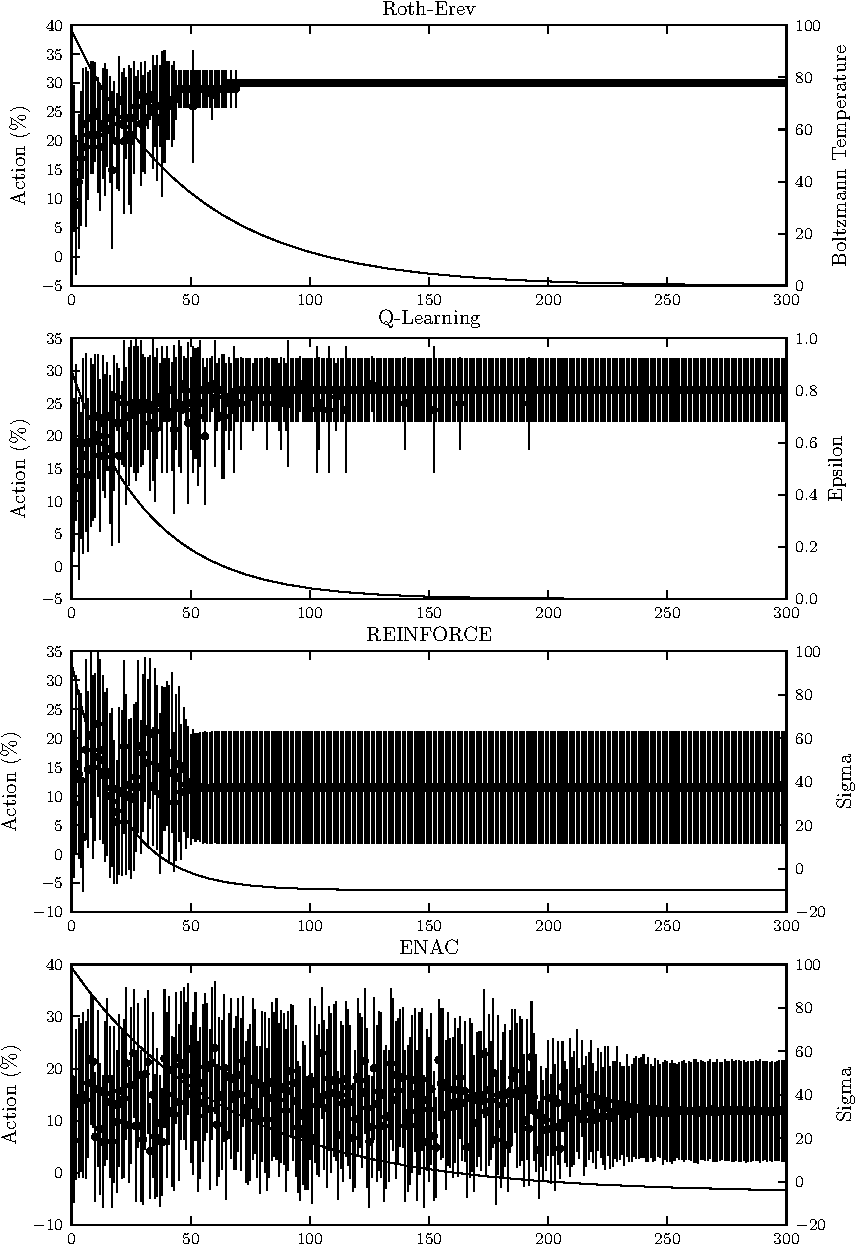
\includegraphics{figures/fig5_1_action_a1}
  \caption{Average markup for agent 1 and standard deviation over 10 runs.}
  \label{fig:5_1_action_a1}
\end{figure}

\begin{figure}
  \centering
  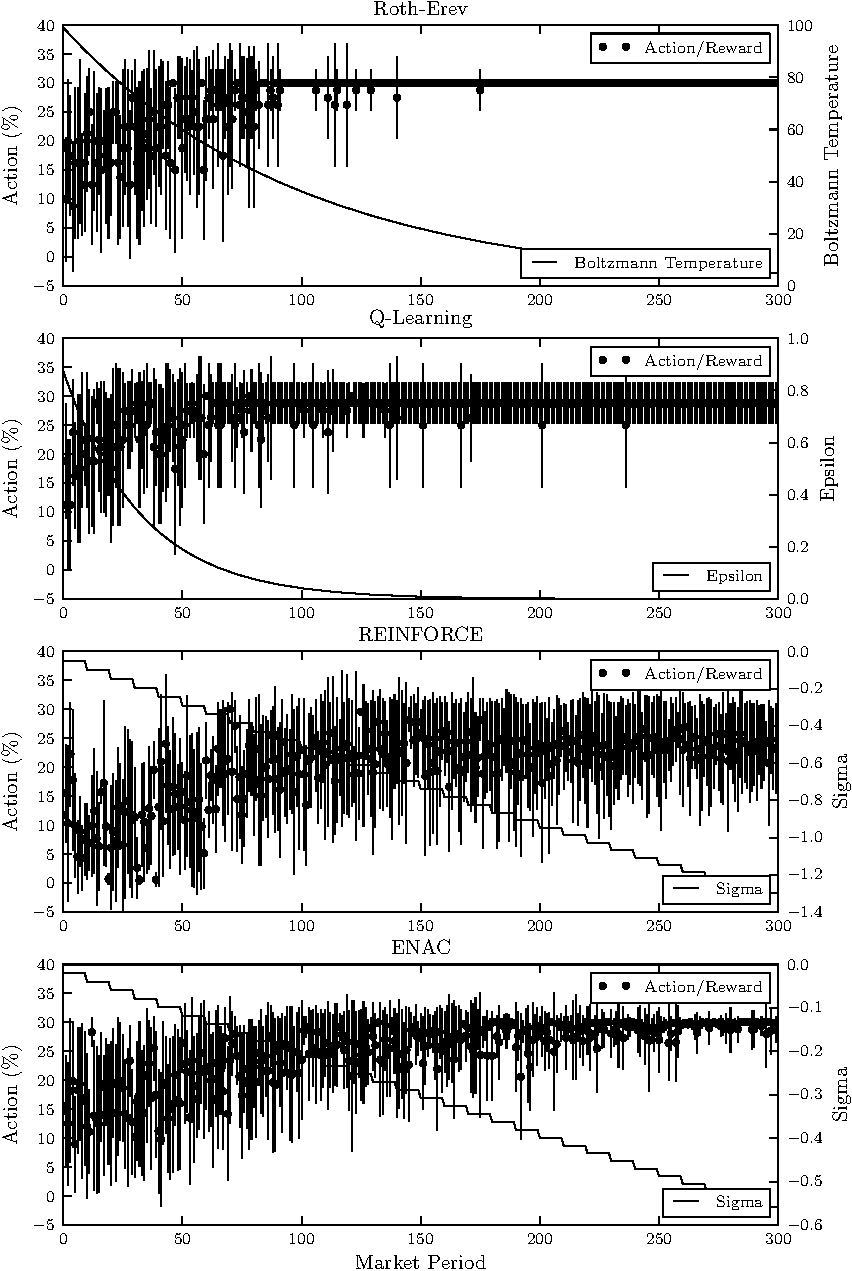
\includegraphics{figures/fig5_1_action_a2}
  \caption{Average markup for agent 2 and standard deviation over 10 runs.}
  \label{fig:5_1_action_a2}
\end{figure}

Figures \ref{fig:5_2_action_a1} and \ref{fig:5_2_action_a2} plot the average
markup for Agent 1 and Agent 2, respectively, under the second price
configuration and again for the variant Roth-Erev, Q-learning, REINFORCE and
ENAC learning methods.  Figures \ref{fig:5_2_reward_a1} and
\ref{fig:5_2_reward_a2} plot the associated average \textit{rewards} for
Agent 1 and Agent 2.  Again the standard deviation and exploration parameter
values are plotted. The plots are vertically aligned and have equal $x$-axis
limits to aid algorithm comparison.
\begin{figure}
  \centering
  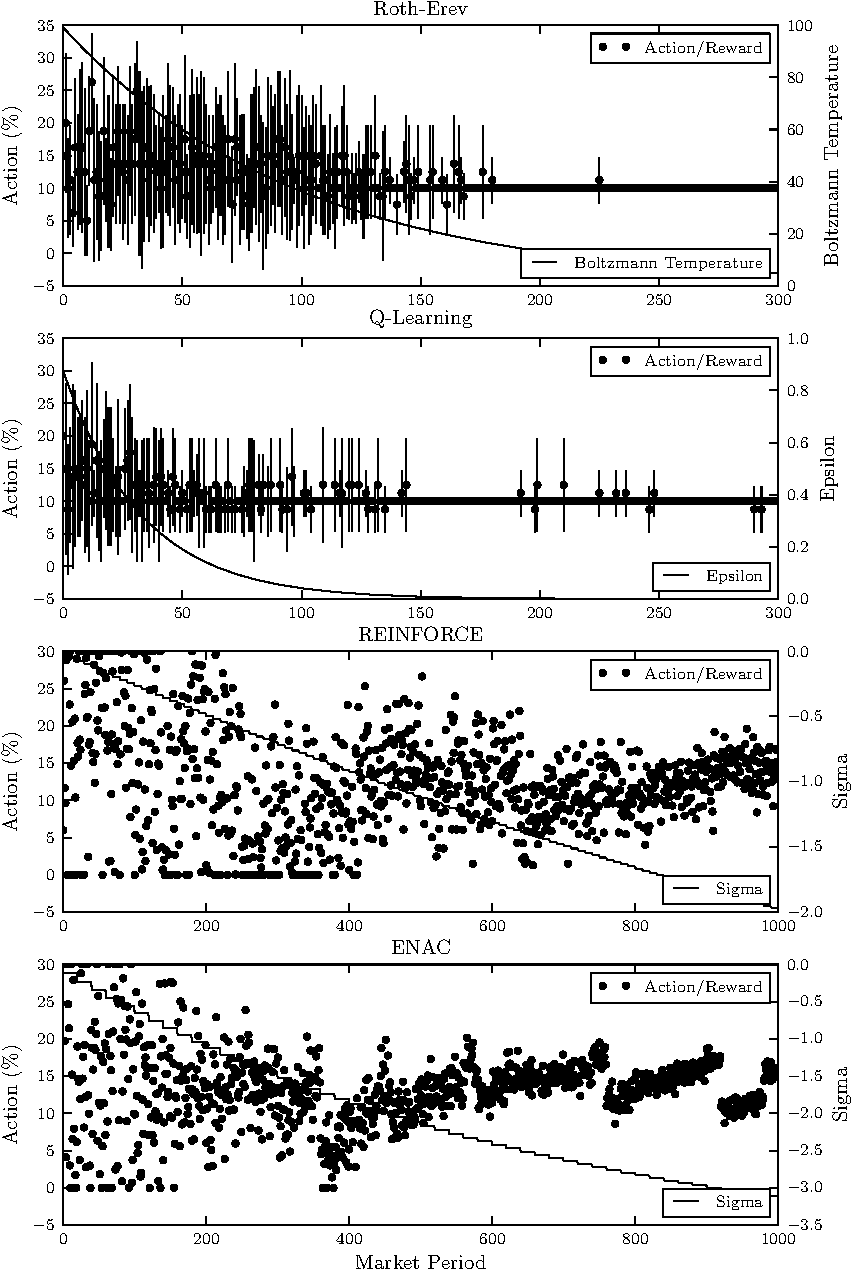
\includegraphics{figures/fig5_2_action_a1}
  \caption{Average markup for agent 1 and standard deviation.}
  \label{fig:5_2_action_a1}
\end{figure}
\begin{figure}
  \centering
  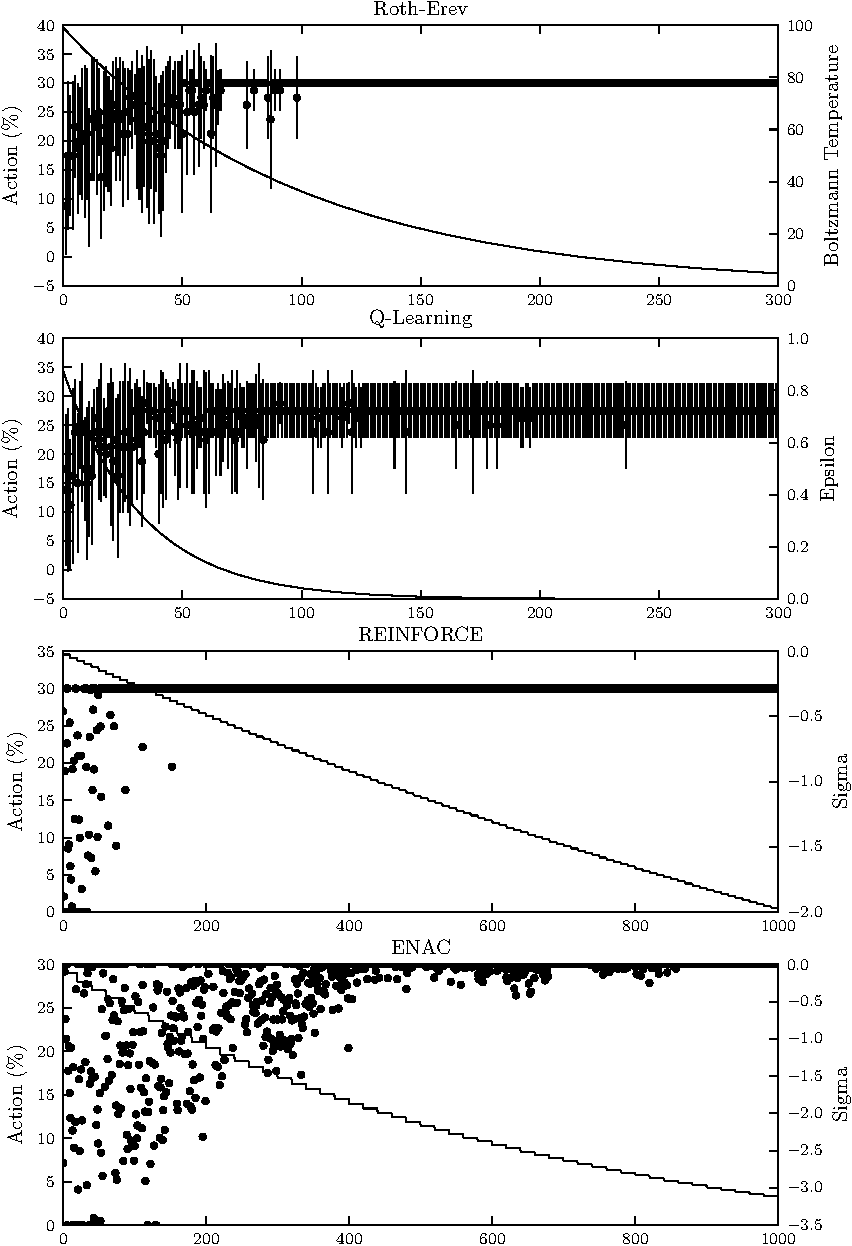
\includegraphics{figures/fig5_2_action_a2}
  \caption{Average markup for agent 2 and standard deviation.}
  \label{fig:5_2_action_a2}
\end{figure}
\begin{figure}
  \centering
  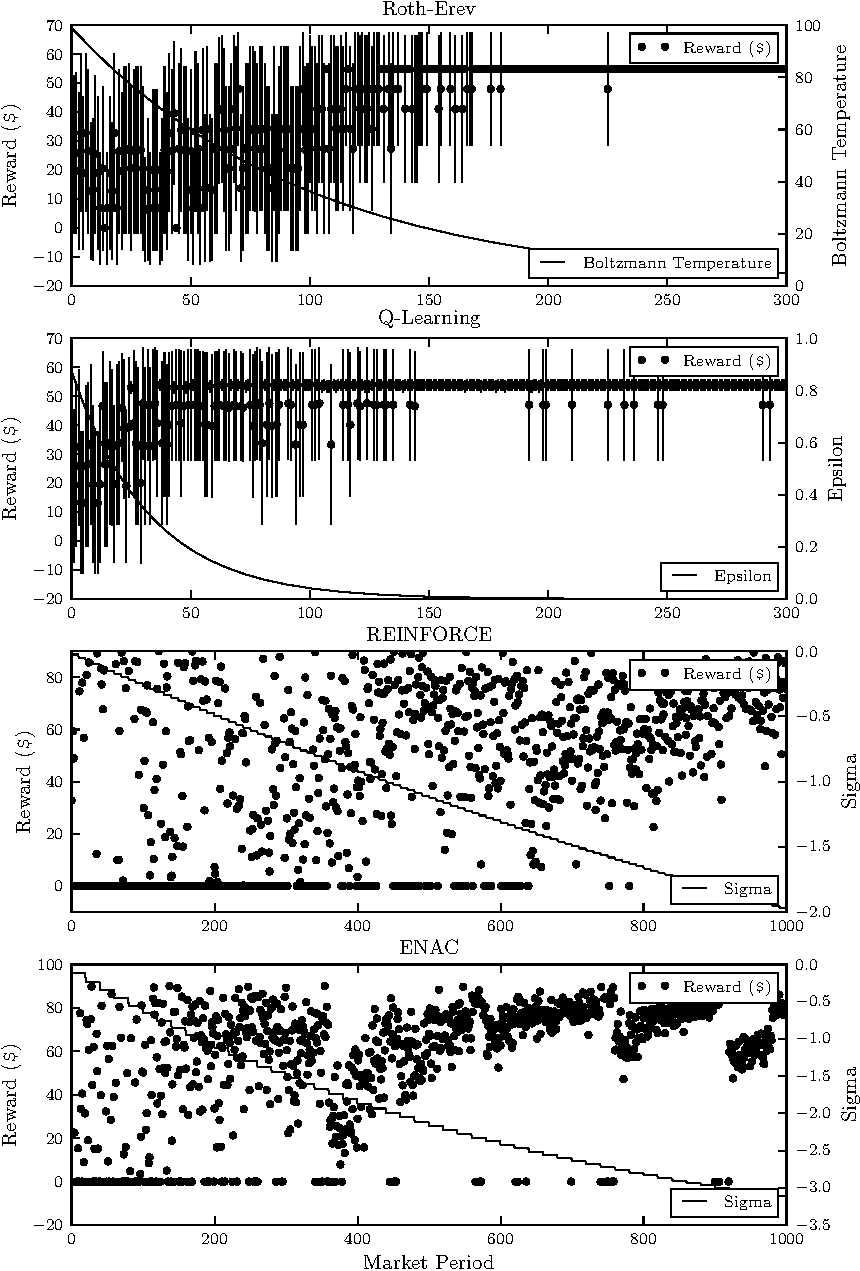
\includegraphics{figures/fig5_2_reward_a1}
  \caption{Average reward for agent 1 and standard deviation.}
  \label{fig:5_2_reward_a1}
\end{figure}
\begin{figure}
  \centering
  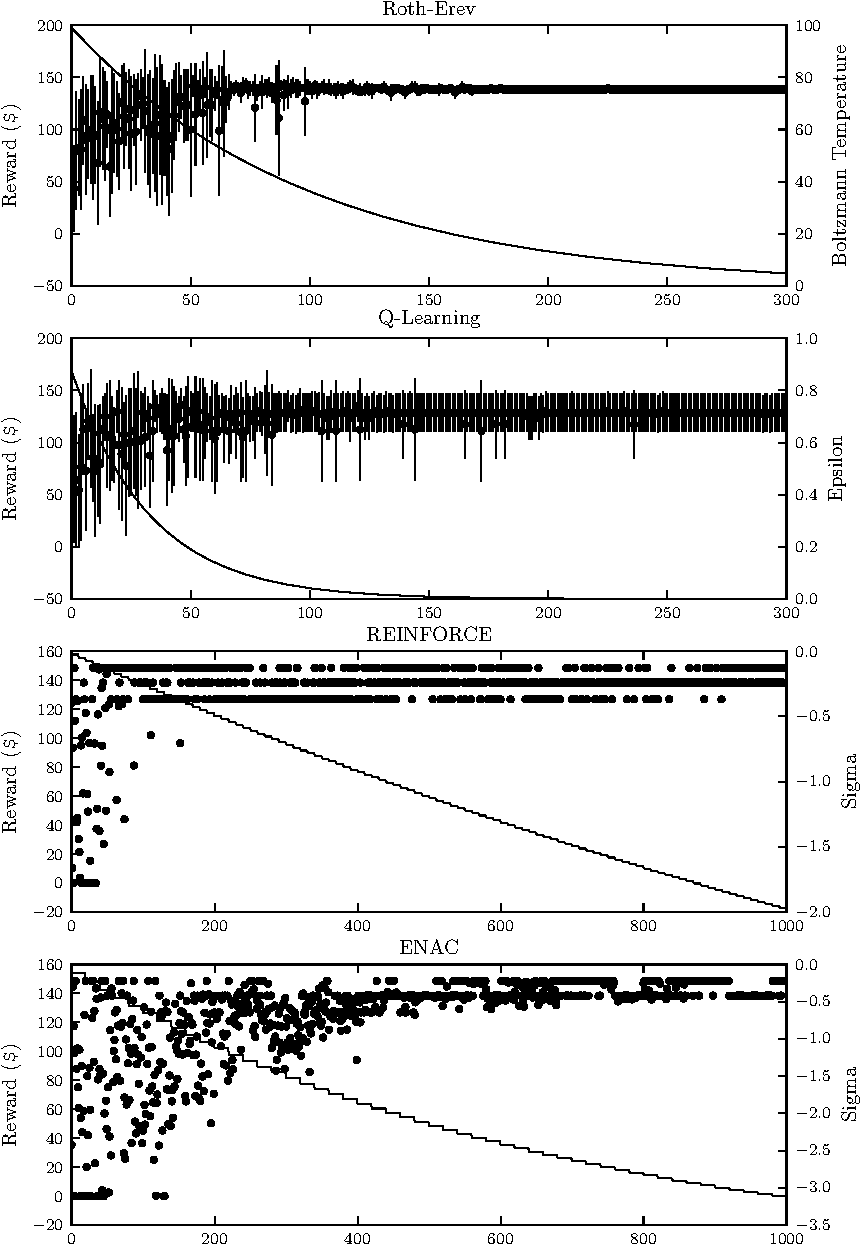
\includegraphics{figures/fig5_2_reward_a2}
  \caption{Average reward for agent 2 and standard deviation.}
  \label{fig:5_2_reward_a2}
\end{figure}

\section{Discussion and Critical Analysis}
Under the first generator price configuration the agents face a simple
control task and receive a clear reward signal that is directly proportional to
their markup action.  The results show that all of the methods consistently
converge to the point of Nash equilibrium.  A multitude of parameter and nerual
network structure variations could be investigated and a sea of similar
plots would be produced.  The author's experience is that the speed of
convergence is largely determined by the rate at which the exploration parameter value is reduced.
The policy gradient methods are sensitive to high learning rate parameter
values, but make only very small policy adjustments if this parameter is set
too low. All of the plots for REINFORCE and ENAC show that the methods only converge to a
stable policy if the exploration parameter $\sigma$ is manually reduced to
below approximately~$-2$.

The second pricing configuration provides a more challenging control problem in
which there is some interdependence between the agent's rewards and where
Agent~1 must learn to undercut the passive agent.  The results show that the
variant Roth-Erev and Q-learning methods both consistantly learn their optimal
policy and converge to the Nash equilibrium.  It should be noted that Agent~1
can markup its marginal price by slightly more than 10\% and still undercut
the passive agent, but these methods are restricted to discrete actions.

When using REINFORCE or ENAC, Agent~2 tends also to learn to maximise its
markup, but less consistantly.  Agent~1 typically learns to undercut the
passive agent, but does not converge to a consistant value.  The problem is
similar to the cliff-edge walking problems often used as benchmarks in
reinforcement learning research and may be difficult to approximate a policy
for using a small number of $\tanh$ functions. It may be possible to improve
the performance of these agents through more educated policy function
approximator design, but these methods are not really intended for operation in
such simple environments.

This experiment confirms the convergence to a Nash equilibrium of the
Q-learning methods that is published in \citeA{krause:nash06} and, to a degree,
extends the conclusion to policy gradient methods.  The results show that
while these methods do converge to the same or similar policies as the
Q-learning and Roth-Erev methods, they do not exhibit the same level of
consistency.  Value function based methods or the Roth-Erev method may be the
most suitable choice of algorithm in the simple electricity market simulations
typlically found in the literature.

\section{Summary}
The simulations conducted here do not exploit any of
the abilities of policy gradient methods to utilise multi-dimensional
continuous state information and their behaviour in more complex environments
must be examined.

%\section{Summary}


% \chapter{Competitive Power Trade}
% Having compared the learning methods in a one-player context, this section
% describes the method used to pit them against one and other and compare their
% performance.
%
% \section{Aims \& Objectives}
% Competition is fundamental to markets and this experiment aims to compare
% learning methods in a complex dynamic market environment with multiple
% competing participants.  The objective is to compare:
% \begin{itemize}
%   \item Performance, in terms of profitability, over a finite number of
%   periods,
%   \item Profitability when trading both active and reactive power.
%   \item Consistency of profit making and,
%   \item Sensitivity to algorithm parameter changes.
% \end{itemize}
%
% \section{Method of Simulation}
% Figure X illustrates the structure of the six bus power system model, from
% \cite{wood:pgoc}, with three generators and fixed demand at three of the buses
% used to provide a dynamic environment with typical system values.  Bus,
% branch and generator attribute values are stated in Tables X, Y, Z,
% respectively.  Three learning methods are compared in six simulations
% encapsulating all method--generator combinations.
%
% A price cap $c_{cap}$ of twice the marginal cost of the most expensive generator
% at full capacity is set by the market.  The simulations are repeated for with agents
% actions composing both price and quantity and with just price.  For the
% value-function methods, the state is defined by the market clearing price from
% the previous period, divided equally into $x_s$ discrete states between $0$ and
% $c_{cap}$.  The state vector $s_t$ for the policy gradient methods consists of
% the market clearing price and generator set-point from the previous period.
% \begin{equation}
% s_t =
% \begin{bmatrix}
% c_{mcp}\\
% p_g
% \end{bmatrix}
% \end{equation}
% The script used to conduct the simulation is provided in Listing X.

\chapter{System Constraint Exploitation}
\label{ch:exploitation}
% One of the main features of agents using policy gradient learning methods and
% artifical neural networks for policy function approximation is their ability to
% accept many signals of continuous sensor data.  This section describes an
% experiment in which the power system is severly constrained for certain
% periods, resulting in elevated nodal marginal prices in particular areas.  The
% methods are tested in their ability to exploit these constraints and improve
% their total accumulated reward.
This chapter explores the exploitation of constraints in electric power
system models by agents whose behaviour is determined by reinforcement learning
algorithms.  Value function based and policy gradient methods are compared
using the IEEE Reliability Test System, with dynamic loads and probabilistic
transmission line outages.

\section{Introduction}
Having explored the basic properties of various learning methods in
Chapter~\ref{ch:learningtotrade}, this experiment examines them under a complex dynamic scenario.  Policy gradient methods have been used in robotic control
applications with multi-dimensional, continuous state and action spaces, and
exhibit a degree of robustness to sensor noise.  In this experiment,
these features are explored in the context of learning to trade power.

Control of a portfolio of generators using continous sensor data from
simulations of a standard test power system model with realisitic load dynamics
is examined.  To force the system into a constrained state at certain times, transmission line outages are simualated according to the probabilities given in Table Z.  By
observing the actions taken and the reward received by an agent during these
periods it is examined if these methods can be used to exploit such
occurances.

\section{Aims and Objectives}
This experiment aims to compare the operation of learning methods in dynamic
electric power system environments.  Specifically, the objective are to
determine:
\begin{itemize}
  \item If policy gradient methods can be used to achieve greater profit under
  dynamic loading conditions.
  \item If policy gradient methods can exploit outages and the resulting system
  constraints to further increased profit.
  \item The value of using AC optimal power flow formulations in agent base
  electricity market simulation.
\end{itemize}
Meeting these objectives aims to demonstrate the value of policy gradient
methods in electricity market participant modelling.

\section{Method of Simulation}
The learning methods are compared by repeating the same simulation with
different types of algorithm in-place.  Some simplification of the state
and action domains for the value function based methods is required, but the
portfolios of generation and load profiles are constant.

The IEEE Reliability Test System \cite{ieee79rts} provides the power system
model, load profiles and outage probabilities used in each simulation.  The
model has 24 bus locations, connected by 32 transmission lines, 4 transformers
and 2 underground cables.  The transformers tie together two system areas at
230kV and 138kV.  The model has 32 generators of 9 different types (See Table
X) with a total capacity of 3.45GW and load at 17 locations, totalling 2.85GW.
Generator costs are quadratic functions of output, defined by the parameters in
Table Y.  Figure X plots the cost functions for each type of generator over
their production range and illustrates their categorisation by fuel type.  Data
for the model is provided in Appendix \ref{adx:ieee_rts} and the connectivity
of branches and the location of generators and loads is illustrated in
Figure~Y.

\begin{figure}
  \centering
  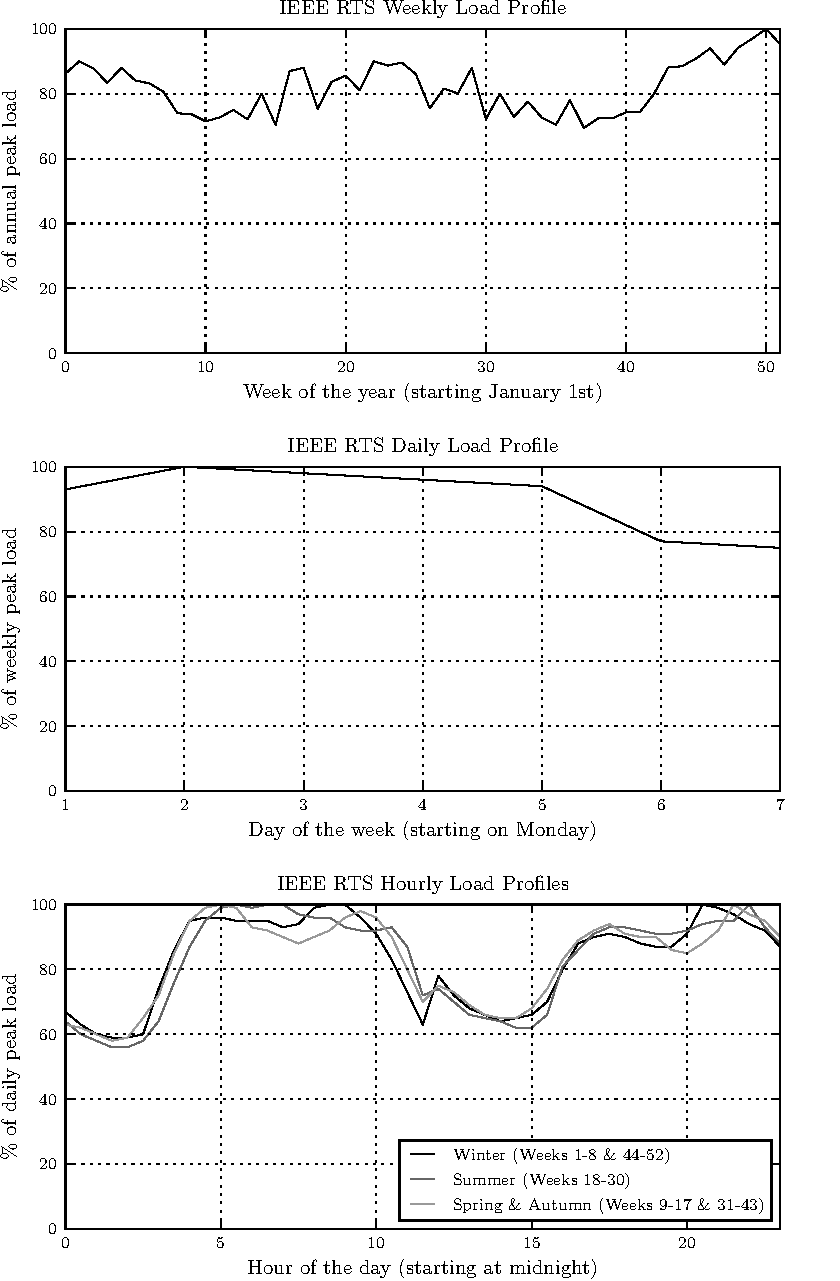
\includegraphics{figures/ieee_rts_profiles}
  \caption{Hourly, daily and weekly load profile plots from the IEEE
  Reliability Test System}
  \label{fig:iee_rts_profiles}
\end{figure}

The generating stock is divided into 5 portfolios, as listed in Table Z, that
are each endowed to a learning agent.  The synchronous generator is associated
with a passive agent that always offers at marginal cost i.e.~\$/MWh~0.
Markups of offer price are restricted a maximum of 30\% and discrete markup
steps of 10\% are defined for value function based methods.

%\newcommand{\generatorunit}[3]{
  \node[circle,draw,thick,minimum width=6mm,#3] (#1) at (#2) {};
  \draw[thick] ($(#2)-(2mm,0)$) sin ++(1mm,1mm) cos ++(1mm,-1mm)
  sin ++(1mm,-1mm) cos ++(1mm,1mm);
}

\begin{figure}
\centering
\small
\begin{tikzpicture}[thick,label distance=0mm]
  \tikzstyle{busbar} = [rectangle,draw,fill=black!50,inner sep=0pt];
  \tikzstyle{hbus} = [busbar,minimum width=10mm,minimum height=2pt];
  \tikzstyle{vbus} = [busbar,minimum width=2pt,minimum height=10mm];
  \tikzstyle{overhead} = [-,thick];
  \tikzstyle{cable} = [thick];
  \tikzstyle{trxcircle} = [circle,draw=black,inner sep=0pt,minimum width=5mm];
  \tikzstyle{every pin edge}=[-,shorten <=1pt,thin];

\node[hbus,minimum width=15mm,label=left:Bus 1] (bus1) at (5,0) {};
\node[hbus,minimum width=15mm,label=right:Bus 2] (bus2) at (7,0) {};
\node[hbus,label=right:Bus 3] (bus3) at (0,6) {};
\node[vbus,label=above:Bus 4] (bus4) at (3,4) {};
\node[vbus,label=above:Bus 5] (bus5) at (6.5,3) {};
\node[vbus,label=above:Bus 6] (bus6) at (12,5.3) {};
\node[hbus,label=right:Bus 7] (bus7) at (11,0.5) {};
\node[vbus,label=above:Bus 8] (bus8) at (12,3) {};
\node[hbus,minimum width=20mm,label=left:Bus 9] (bus9) at (5,6) {};
\node[hbus,minimum width=20mm,label=right:Bus 10] (bus10) at (8,6) {};
\node[hbus,minimum width=20mm,label=left:Bus 11] (bus11) at (5,8) {};
\node[hbus,minimum width=20mm,label=right:Bus 12] (bus12) at (8,8) {};
\node[vbus,label={[xshift=-4mm]below:Bus 13}] (bus13) at (12,10) {};
\node[vbus,label=above:Bus 14] (bus14) at (3.5,11.5) {};
\node[hbus,minimum width=20mm,label=right:Bus 15] (bus15) at (0.5,12) {};
\node[hbus,minimum width=15mm,label=right:Bus 16] (bus16) at (0,14) {};
\node[vbus,minimum height=20mm,label=above:Bus 17] (bus17) at (-1,16) {};
\node[hbus,minimum width=20mm,label=right:Bus 18] (bus18) at (2,18) {};
\node[hbus,label=below right:Bus 19] (bus19) at (4.5,14) {};
\node[hbus,minimum width=15mm,label=below right:Bus 20] (bus20) at (7,14) {};
\node[hbus,minimum width=25mm,label=right:Bus 21] (bus21) at (5,17) {};
\node[hbus,label=right:Bus 22] (bus22) at (9,17) {};
\node[vbus,minimum height=15mm,label=above:Bus 23] (bus23) at (11,14.55) {};
\node[hbus,label=right:Bus 24] (bus24) at (0,8) {};

% Branch 1-2.
\draw[cable] ([xshift=5mm] bus1.north) -- ++(0,5mm) node[xshift=5mm,above]
{cable} -| ([xshift=-5mm] bus2.north);
% Branch 1-3.
\draw[overhead] ([xshift=-5mm] bus1.north) -- ([xshift=-5mm,yshift=5mm]
bus1.north) -- ([xshift=0mm,yshift=-5mm] bus3.south) -- (bus3.south);
% Branch 1-5.
\draw[overhead] (bus1.north) |- (bus5.west);
% Branch 2-4.
\draw[overhead] (bus2.north) -- ([yshift=5mm] bus2.north) -- ([xshift=5mm]
bus4.east) -- (bus4.east);
% Branch 2-6.
\draw[overhead] ([xshift=5mm] bus2.north) -- ([xshift=5mm,yshift=5mm]
bus2.north) -- ([xshift=-5mm,yshift=-3mm] bus6.west) -- ([yshift=-3mm]
bus6.west);
% Branche 3-9.
\draw[overhead] ([xshift=3mm] bus3.south) -- ++(0,-5mm) -| ([xshift=-5mm]
bus9.south);
% Branch 3-24.
\draw node[trxcircle,yshift=-1mm,above of=bus3] (t3-24p) {};
\draw node[trxcircle,yshift=1mm,above of=bus3] (t3-24s) {};
\draw[overhead] (bus3.north) -- (t3-24p.south);
\draw[overhead] (t3-24s.north) -- (bus24.south);
% Branch 4-9.
\draw[overhead] ([yshift=3mm] bus4.east) -- ([xshift=5mm,yshift=3mm] bus4.east)
-- ([yshift=-5mm] bus9.south) -- (bus9.south);
% Branch 5-10.
\draw[overhead] (bus5.east) -| (bus10.south);
% Branch 6-10.
\draw[overhead] (bus6.west) -| node[above right] {cable} ([xshift=5mm]
bus10.south);
% Branch 7-8.
\draw[overhead] ([xshift=-3mm] bus7.north) |- ([yshift=-3mm] bus8.west);
% Branch 8-9.
\draw[overhead] (bus8.west) -- ([xshift=-5mm] bus8.west) --
([xshift=5mm,yshift=-5mm] bus9.south) -- ([xshift=5mm] bus9.south);
% Branch 8-10;
\draw[overhead] ([yshift=3mm] bus8.west) -- ([xshift=-5mm,yshift=3mm]
bus8.west) -- ([xshift=-5mm,yshift=-10mm] bus10.south) -- ([xshift=-5mm]
bus10.south);
% Branch 9-11.
\draw node[trxcircle,yshift=-1mm,xshift=-5mm,above of=bus9] (t9-11p) {};
\draw node[trxcircle,yshift=1mm,xshift=-5mm,above of=bus9] (t9-11s) {};
\draw[overhead] ([xshift=-5mm] bus9.north) -- (t9-11p.south);
\draw[overhead] (t9-11s.north) -- ([xshift=-5mm] bus11.south);
% Branch 9-12.
\draw node[trxcircle,yshift=-1mm,xshift=-5mm,node distance=7mm,below of=bus12]
(t9-12p) {};
\draw node[trxcircle,yshift=1mm,xshift=-5mm,node distance=7mm,below of=bus12]
(t9-12s) {};
\draw[overhead] ([xshift=5mm] bus9.north) -- ([xshift=5mm,yshift=3mm]
bus9.north) -- ([yshift=-3mm] t9-12p.south) -- (t9-12p.south);
\draw[overhead] (t9-12s.north) -- ([xshift=-5mm] bus12.south);
% Branch 10-11.
\draw node[trxcircle,yshift=-1mm,xshift=5mm,node distance=7mm,below of=bus11]
(t10-11p) {};
\draw node[trxcircle,yshift=1mm,xshift=5mm,node distance=7mm,below of=bus11]
(t10-11s) {};
\draw[overhead] ([xshift=-5mm] bus10.north) -- ([xshift=-5mm,yshift=3mm]
bus10.north) -- ([yshift=-3mm] t10-11p.south) -- (t10-11p.south);
\draw[overhead] (t10-11s.north) -- ([xshift=5mm] bus11.south);
% Branch 10-12.
\draw node[trxcircle,yshift=-1mm,xshift=5mm,above of=bus10] (t10-12p) {};
\draw node[trxcircle,yshift=1mm,xshift=5mm,above of=bus10] (t10-12s) {};
\draw[overhead] ([xshift=5mm] bus10.north) -- (t10-12p.south);
\draw[overhead] (t10-12s.north) -- ([xshift=5mm] bus12.south);
% Branch 11-13.
\draw[overhead] ([xshift=5mm] bus11.north) -- ([xshift=5mm,yshift=5mm]
bus11.north) -- ([xshift=-5mm] bus13.west) -- (bus13.west);
% Branch 11-14.
\draw[overhead] ([xshift=-5mm] bus11.north) |- ([yshift=-3mm] bus14.east);
% Branch 12-13.
\draw[overhead] ([xshift=-5mm] bus12.north) -- ([xshift=-5mm,yshift=7mm]
bus12.north) -- ([xshift=-5mm,yshift=-3mm] bus13.west) -- ([yshift=-3mm]
bus13.west);
% Branch 12-23.
\draw[overhead] ([xshift=5mm] bus12.north) |- ([yshift=-5mm] bus23.west);
% Branch 13-23.
\draw[overhead] ([yshift=3mm] bus13.west) -- ([xshift=-5mm,yshift=3mm]
bus13.west) |- ([yshift=-5mm] bus23.east);
% Branch 14-16.
\draw[overhead] ([yshift=3mm] bus14.west) -- ([xshift=-6mm,yshift=3mm]
bus14.west) |- ([xshift=5mm,yshift=-5mm] bus16.south) -- ([xshift=5mm]
bus16.south);
% Branch 15-16.
\draw[overhead] ([xshift=-5mm] bus15.north) -- (bus16.south);
% Branches 15-21.
\draw[overhead] (bus15.north) -- ([yshift=5mm] bus15.north) -- ([yshift=-10mm]
bus21.south) -- (bus21.south);
\draw[overhead] ([xshift=5mm] bus15.north) -- ([xshift=5mm,yshift=5mm]
bus15.north) -- ([xshift=5mm,yshift=-10mm] bus21.south) -- ([xshift=5mm]
bus21.south);
% Branch 15-24.
\draw[overhead] ([xshift=-5mm] bus15.south) -- (bus24.north);
% Branch 16-17.
\draw[overhead] ([xshift=-5mm] bus16.north) |- ([yshift=-5mm] bus17.east);
% Branch16-19.
\draw[overhead] ([xshift=5mm] bus16.north) -- ([xshift=5mm,yshift=5mm]
bus16.north) -| ([xshift=-3mm] bus19.north);
% Branch 17-18.
\draw[overhead] ([yshift=5mm] bus17.east) -| ([xshift=-5mm] bus18.south);
% Branch 17-22.
\draw[overhead] (bus17.east) -- ([xshift=20mm] bus17.east) -- ([xshift=20mm,
yshift=-5mm] bus17.east) -| ([xshift=3mm] bus22.south);
% Branches 18-21.
\draw[overhead] (bus18.south) -- ([yshift=-20mm] bus18.south) -|
([xshift=-5mm] bus21.south);
\draw[overhead] ([xshift=5mm] bus18.south) -- ([xshift=5mm,yshift=-15mm]
bus18.south) -| ([xshift=-10mm] bus21.south);
% Branches 19-20.
\draw[overhead] (bus19.north) -- ([yshift=10mm] bus19.north) -|
([xshift=-1.5mm] bus20.north);
\draw[overhead] ([xshift=3mm] bus19.north) -- ([xshift=3mm,yshift=5mm]
bus19.north) -| ([xshift=-4.5mm] bus20.north);
% Branches 20-23.
\draw[overhead] ([xshift=1.5mm] bus20.north) |- ([yshift=5mm] bus23.west);
\draw[overhead] ([xshift=4.5mm] bus20.north) |- (bus23.west);
% Branch 21-22.
\draw[overhead] ([xshift=10mm] bus21.south) -- ([xshift=10mm,yshift=-7.5mm]
bus21.south) -| ([xshift=-3mm] bus22.south);

% Generator @ Bus 1.
\generatorunit{gen1}{4.5,-0.8}{label=left:192 MW,pin={[pin distance=12mm,text
centered,text width=10.5mm]165:2$\times$U20 2$\times$U76}};
\draw[overhead] ([xshift=-5mm] bus1.south) -- (gen1.north);
% Generator @ Bus 2.
\generatorunit{gen2}{7.5,-0.8}{label=right:192 MW,pin={[pin distance=12mm,text
centered,text width=10.5mm]15:2$\times$U20 2$\times$U76}};
\draw[overhead] ([xshift=5mm] bus2.south) -- (gen2.north);
% Generator @ Bus 7.
\generatorunit{gen3}{11,-0.3}{label=right:300 MW,pin=below:3$\times$U100};
\draw[overhead] (bus7.south) -- (gen3.north);
% Generator @ Bus 13.
\generatorunit{gen4}{12.3,10.9}{label=above:591 MW,pin={[pin distance=8mm]
left:3$\times$U197}};
\draw[overhead] ([yshift=3mm] bus13.east) -- ([yshift=3mm,xshift=2.5mm]
bus13.east) -- (gen4.south);
% Generator @ Bus 14.
\generatorunit{gen5}{4.3,11.8}{label={[text justified,text
width=15mm]right:Synch. Cond.}}; \draw[overhead] ([yshift=3mm] bus14.east) --
(gen5.west);
% Generator @ Bus 15.
\generatorunit{gen6}{0.5,11.2}{label={[text centered,text width=10mm]below:215 MW},
pin={[pin distance=5mm,text centered,text width=15mm]-70:5$\times$U12
1$\times$U155}}; \draw[overhead] (bus15.south) -- (gen6.north);
% Generator @ Bus 16.
\generatorunit{gen7}{0.0,15}{label=right:155 MW};
\draw[overhead] (bus16.north) -- (gen7.south);
% Generator @ Bus 18.
\generatorunit{gen8}{1.5,18.8}{label=left:400 MW,pin={[pin distance=6mm]below
left:Nuclear}}; \draw[overhead] ([xshift=-5mm] bus18.north) -- (gen8.south);
% Generator @ Bus 21.
\generatorunit{gen9}{5,17.8}{label=right:400 MW,pin={above right:Nuclear}};
\draw[overhead] (bus21.north) -- (gen9.south);
% Generator @ Bus 22.
\generatorunit{gen10}{9,17.8}{label=right:300 MW,pin={above:Hydro, 6$\times$U50}};
\draw[overhead] (bus22.north) -- (gen10.south);
% Generator @ Bus 23.
\generatorunit{gen11}{11.8,15.05}{label=below:660 MW,pin={[text centered,text
width=15mm]above:2$\times$U155 1$\times$U350}};
\draw[overhead] ([yshift=5.05mm] bus23.east) -- (gen11.west);

% Load @ Bus 1.
\draw[loadline] ([xshift=5mm] bus1.south) -- ++(0,-0.8) node[text centered,text
width=10mm,below] {108 MW};
% Load @ Bus 2.
\draw[loadline] ([xshift=-5mm] bus2.south) -- ++(0,-0.8) node[text
centered,text width=10mm,below] {97 MW};
% Load @ Bus 3.
\draw[loadline] ([xshift=-3mm] bus3.south) -- ++(0,-0.8) node[text
centered,text width=10mm,below] {108 MW};
% Load @ Bus 4.
\draw[loadline] ([yshift=-3mm] bus4.east) -- ++(3mm,0) -- ++(0,-0.8)
node[below] {74 MW};
% Load @ Bus 5.
\draw[loadline] ([yshift=-3mm] bus5.east) -- ++(3mm,0) --
++(0,-0.8) node[below] {71 MW};
% Load @ Bus 6.
\draw[loadline] (bus6.east) -- ++(3mm,0) -- ++(0,-0.8) node[below] {136 MW};
% Load @ Bus 7.
\draw[loadline] ([xshift=3mm] bus7.north) -- ++(0,0.8) node[right] {125 MW};
% Load @ Bus 8.
\draw[loadline] (bus8.east) -- ++(3mm,0) -- ++(0,-0.8) node[left] {171 MW};
% Load @ Bus 9.
\draw[loadline] ([xshift=2.5mm] bus9.south) -- ++(0,-1) node[below] {175 MW};
% Load @ Bus 10.
\draw[loadline] ([xshift=7.5mm] bus10.north) -- ++(0,3mm) -- ++(8mm,0)
node[above right] {195 MW};
% Load @ Bus 13.
\draw[loadline] ([yshift=-3mm] bus13.east) -- ++(2.5mm,0) -- ++(0,-1)
node[below] {265 MW};
% Load @ Bus 14.
\draw[loadline] ([yshift=-3mm] bus14.west) -- ++(-3mm,0) -- ++(0,-0.8)
node[below] {194 MW};
% Load @ Bus 15.
\draw[loadline] ([xshift=7mm] bus15.south) -- ++(0,-0.8) node[right]
{317 MW};
% Load @ Bus 16.
\draw[loadline] ([xshift=-5mm] bus16.south) -- ++(0,-0.8) node[text centered,
text width=10mm,below] {100 MW};
% Load @ Bus 18.
\draw[loadline] ([xshift=5mm] bus18.north) -- ++(0,0.8) node[right] {333 MW};
% Load @ Bus 19.
\draw[loadline] (bus19.south) -- ++(0,-0.8) node[right] {181 MW};
% Load @ Bus 20.
\draw[loadline] (bus20.south) -- ++(0,-0.8) node[below] {128 MW};

% Area voltage labels.
\node[draw] at (1,2) {\normalsize{138 kV}};
\node[draw] at (6.5,10.3) {\normalsize{230 kV}};

\end{tikzpicture}
\caption{IEEE Reliability Test System}
\label{fig:ieee79rts}
\end{figure}

\section{Simulation Results}
\section{Discussion and Critical Analysis}
\label{sec:discuss}
\section{Summary}


% State hypothesis. Further Work. Restate contribution.
\chapter{Conclusions and Further Work}
\label{ch:conclusion}
This final chapter summarises the conclusions that can be drawn from the
results presented in this thesis and gives some ideas for directing further
research.

\section{Summary Conclusions}
This thesis has introduced the use of policy gradient reinforcement learning
algorithms in modelling strategies of electricity market participants. Over
the last two decades, competitive markets have become an essential component of
electricity supply industries in many large countries.  They will play an
important role in the future as the world population continues to grow and
finite primary energy fuel resources become increasingly scarce.  Electric
energy trade requires a unique market design, but radical architecture changes
can not be experimented with on real systems.

Computational simulation is a well established technique for evaluating market
design concepts and agent-based simulation is an approach that allows large
complex systems to be modelled.  There are many examples of learning algorithms
being used to model electricity market participants in the literature, but
policy gradient methods have not been previously applied.  These
methods use function approximation techniques to operate in environments
with state and actions spaces that are continuous, discrete or mixed and have
been successfully applied in robot control and other problems.

To examine the properties of policy gradient methods and compare their
performance with previously applied value function based methods, a modular
simulation framework has been defined and implemented.  The framework uses a
power exchange auction market model with nodal marginal pricing to provide an
environment in which agents can \textit{learn to trade power} competitively.

The framework has first been used in a simulation that compares the convergence
to Nash equilibria of four different learning algorithms.  The simulation
structures reproduced the findings of \citeA{krause:nash06} and presented
similar results for policy gradient methods.  Policy gradient methods were
found: to exhibit very different characteristics to value function based
methods, to require a larger number of interactions before learning an optimal
policy and to require low learning rate and exploration rate decay parameters
for complex equilibria to be approached.

In a second simulation the framework was used to compare the same algorithms in
a complex dynamic electricity trading environment.  A reference electric power
system model, designed for reliability analysis, was used to provide a
realistic environment of a reasonable size.  The algorithms were compared in
their ability to observe and exploit constraints in the system as loads followed
an hourly profile.  It was not found that policy gradient methods could use
additional bus voltage data to achieve greater performance than an action-value
function based method or a stateful variant of the Roth-Erev technique.
However, they were shown to learn effective strategies under noisy dynamic
conditions and to improve performance using complex continuous state
representations.

In conclusion, policy gradient methods are a valid option for modelling the
strategies of electricity market participants.  They can use profit feedback
from an electricity market model to adjust the parameters of a policy function
approximator in the direction of increased reward.  Function approximators allow
market participants to be modelled using agents that accept complex power system
state data and produce offers for diverse portfolios of generators with
price markups applied and capacity withheld.  This thesis has compared
a selection of techniques for participant modelling and provides guidance for
algorithm and parameter selection.
% It has been how even moderately complex electricity market simulations produce
% state and action spaces that are too large for value function based methods to
% explore. Policy gradient methods have been shown to produce consistent
% behaviour in increasingly complex dynamic trading problems.
Further development of the ideas in this thesis could allow advanced learning
algorithms to be used to support the decisions made by traders in electricity
markets or in fully automated energy trade.

\section{Further Work}
\label{sec:furtherwork}
This final section highlights some of the shortcomings of the methodology
presented in this thesis and explains how the models could be further developed.
It introduces some alternative learning algorithms that might also be used to
simulate electricity market participant behaviour.
% Also, two new reinforcement learning problem formulations are defined that
% concern two highly pertinent issues in electric power Engineering.
It explains how a model formulated using data from National Grid Ltd.~could be
used in practical simulations of the UK electricity market and describes some
other possibilities for using AC optimal power flow in agent-based electric
power market simulation.

\subsection{Parameter Sensitivity and Delayed Reward}
The simulations presented in this thesis use typical algorithm parameter choices
that are either the default values from PyBrain or inspired by the literature.
Alternative function approximation and back-propagation techniques, such as
decision trees, (neuro-)fuzzy methods \cite{jang93anfis} and RProp
\cite{riedmiller93}, could be investigated in the future. In reinforcement
learning, parameter sensitivity analysis is often conducted by the algorithm
developers using standard benchmark problems (such as mazes or pole balancing
problems \cite{schaul:2010}) that are familiar to researchers in artificial
intelligence and allow results to be compared. The shortage of published results
and lack of standardised electricity trading models might limit the benefits of
using this problem for general parameter sensitivity analysis.

The reward signals received by agents in all of the simulations presented in
this thesis result directly from the agent's previous action.  In
practice, a market settlement process would introduce delays to payments for
electricity production. Time did not permit value function based methods with
eligibility traces (See Section \ref{sec:eligibility}) to be compared with
policy gradient methods, but the ability to learn under delayed reward is a
fundamental part of both reinforcement learning and market trade and deserves
investigation in this context.

% Actions in previous states not only effect the reward signal, but the current
% range of possible actions.  The rate at which generator types can ramp up or
% ramp down production is a typical constraining factor in this regard.
% Multi-period optimal power flow formulations may incorporate such constraints,
% but are challenging to implement and solve.

\subsection{Alternative Learning Algorithms}
This thesis has concentrated on traditional value function based methods, the
Roth-Erev technique and two policy gradient reinforcement learning methods.
However, there are other learning algorithms that have been published recently
that could also be used in electric power trade simulations.

\citeA{riedmiller05nfq} presented Neuro-Fitted Q-Iteration (NFQ)
algorithms that attempt to overcome many of the problems experienced when implementing
Q-learning methods with value function approximation using neural networks.
They store all transition experiences and perform off-line updates using
supervised learning techniques such as RProp \cite{riedmiller93}.  The method
has been shown to be robust against parameterisation and to learn quickly in
standard benchmark tests and real-world applications \cite{kietzmann09}.

The GQ$(\lambda)$ algorithm by \citeA{maei10} is another extension of Q-learning
for operation in continuous environments.  Convergence guarantees have been
shown and the scaling properties suggest the method is suitable for large-scale
reinforcement learning applications.
% A software implementation of GQ$(\lambda)$
% has been developed and recently made available as open source.

Four new Natural Actor-Critic algorithms have been presented by
\citeA{bhatnagar09}. Like ENAC, they use function approximation techniques and
are suitable for large-scale applications of reinforcement learning.  Three of
the algorithms are extensions to ENAC, but are fully incremental: the gradient
computation is never reset while the policy is updated at every simulation step.
 The authors state a need to assess the ultimate utility of these algorithms
through application in real-world problems.

This thesis provides a framework that would allow implementations of these
algorithms to be assessed and used to research aspects of electricity
markets.  As in the simulations described in this thesis, alternative algorithms
could be investigated with the same algorithm being used by all agents at the
same time.  Alternatively, a selection of algorithms could be cycled
around each of the agents in a series of simulations and the ultimate overall
performance examined.

% \subsection{Learning to Optimise Power Flow}
% Two important problems in electric power Engineering, to which to the
% application of advanced reinforcement learning algorithms would be of value,
% are:
% \begin{itemize}
%   \item System optimisation, close to real-time, such that sufficient reserve
%   is allocated to ensure acceptable system security while costs are minimised
%   according to the outcome of the electricity markets, and
%   \item Capital investment planning, both by system operators needing to expand
%   transmission capacity and energy companies wanting to develop new generating
%   plant.
% \end{itemize}
%
%
% As explained in Section \ref{sec:opf}, the objective of the classical optimal
% power flow problem is to find generator set-points that allow all system and
% plant constraints to be satisfied while the total system cost is minimised.
% Interior point methods are possibly the most robust technique for finding
% solutions, but the problem may also be formulated as a continuous
% reinforcement learning task that could be learned by a system operator agent.
% To illustrate the concept, this section presents a preliminary formulation of
% such a task and demonstrates how a system operator agent can use policy
% gradient methods to learn to optimise power flow.
%
% \subsubsection{System Operator Task and Environment}
% The state of the system operator agent's environment is defined simply as a
% demand forecast.  That is, the environment returns a vector of active power
% demand at all system buses.  The initial demand is assumed to be peak and is
% used to normalise the values of the sensor vector to be between $-1$ and $+1$
% before input the the mutil-layer perceptron used for policy function
% approximation.  Simulations are divided into episodes (days) over which the
% demand at each bus follows the profile shown in Figure X.
%
% The agent's action and the output of the policy function approximator is a
% vector of the active power set-points of all generators, excluding the
% generator at the system slack bus.  The set-points are bound by the generator's minimum
% and maximum rated capacity. These bounds are used to denormalise the output
% values from the final Sigmoid layer (that are between $-1$ and $+1$) to give
% valid set-point values.
%
% The new generator set-points are used to form an AC power flow problem that is
% solved using Newton's method \cite{tinney:67}.  The power flow solution
% determines the complex voltage at each bus, the branch power flows and losses,
% the reactive power output of the generators and the active power output of the
% slack bus generator.
%
% The reward is defined as the negative of the sum of all generator costs.  The
% negative of the costs must used since the learning methods attempt to maximise
% reward and the objective is to minimise cost.  The power flow solution does not
% satisfy system constraints, such as voltage limits or generators reactive power
% limits and penalty costs must be applied to the reward so the agent learns to
% obey them.
%
% \subsubsection{Slack Bus Generator Control}
% This initial proof of concept attempts only to enforce the set-point limit on
% the slack bus generator.  The reward is updated according to
% \begin{equation}
% r =
% \begin{cases}
% r + \phi (P_{slack} - P_{max}), & \text{$P_{slack} > P_{max}$} \\
% r, & \text{otherwise}
% \end{cases}
% \end{equation}
% The six bus network model described in Chapter \ref{ch:nashanalysis} is used
% with the coefficients of the generator's quadratic cost functions given in Table X.  Learning is conducted in batch
% mode, with 7 episodes conducted before the parameters of the policy are
% updated.  The system operator agent uses the ENAC learning method with RProp
% gradient descent and an initial value of $\sigma = 50$, which is reduced after
% each simulated week according to $\sigma_{i+1} = 0.5\sigma_i - 2$.
%
% Figure X shows the average output of each generator over 52 simulated weeks of
% control. Plotted in Figure Y is the average total system cost for each week along with
% theoretically optimal values as calcualted by DC and AC optimal power flow
% solvers.  The results show that, with suitable initial experimentation, the
% agent learns to dispatch the generators in the most economically efficient
% manner while controlling the slack bus generators to valid output levels.  The
% average total system cost converges to slightly less that of the optimal
% solution due to the disregard for other constraints, particularly the
% branch flow constraint between buses 2 and 4 which is binding at times of peak
% load.
%
% \subsection{Learning to Plan Investment}

\subsection{UK Transmission System}
Some of the more ambitious agent-based electricity market simulations have used
stylised models of national transmission systems
\cite{cincotti:09,weidlich:06}.  This work has often been motivated by recent
or expected changes to the arrangements in the associated regions.
% The drop in
% oil prices around the time of the global economic crash in 2008 was not
% reflected quickly in energy prices and this amplified concerns over liquiduty
% levels in the UK electricity markets.  Ofgem found competition to be
% sufficient[ref], but the concerns persists and the market arrangements have
% been re-examined under Project Discovery[ref].
In the UK, nine large power stations are due to be decommissioned by 2016 in
accordance with EU Large Combustion Plant Directive \cite{ngt07lcpd}.  Coupled
with obligations, made in the Climate Change Act 2008, to cut greenhouse gas
emissions by 80\% of 1990 levels by 2050, coming years are likely to see major
changes in the way the UK power system is operated.
% The ability of the market to sufficiently incentivize new
% investment in generation that will cover the resulting shortfall is in question.  The concern extends
% to the need for long-term investment in new nuclear power plant that is deemed
% necessary for the UK to meet the legally binding obligations, made in the
% Climate Change Bill, to cut greenhouse gas emissions by 80\% by 2050, compared
% to 1990 levels.
Examination of the situation could be enhanced by advanced participant
behavioural models and accurate electric power system simulations such as those
presented in this thesis.

Figure \ref{fig:ngt_grid} illustrates a model of the UK transmission system that
has been formulated from data provided by the \citeA{ngtsys2010}.  This model
has been converted into PSS/E raw file format and is included with the
code developed for this thesis (See Appendix \ref{sec:pylon}).
% Generator set-points were determined using the state estimator from Pylon
% [Crow].  The power flow results are shown in Figure X and correlate accurately
% with those in [SYS], having a mean variance of X.XX. Cost data for each of the
% aggregated generating units has been estimated from public sources and stored
% in the PSS/E version 30 optimal power flow data file in Appendix
% \ref{sec:nget_opf}.  Execution times for solving this case using DC, AC and
% unit de-commitment optimal power flow are shown in Table X.
\ifthenelse{\boolean{includefigures}}{
	\begin{figure}
	  \centering
	  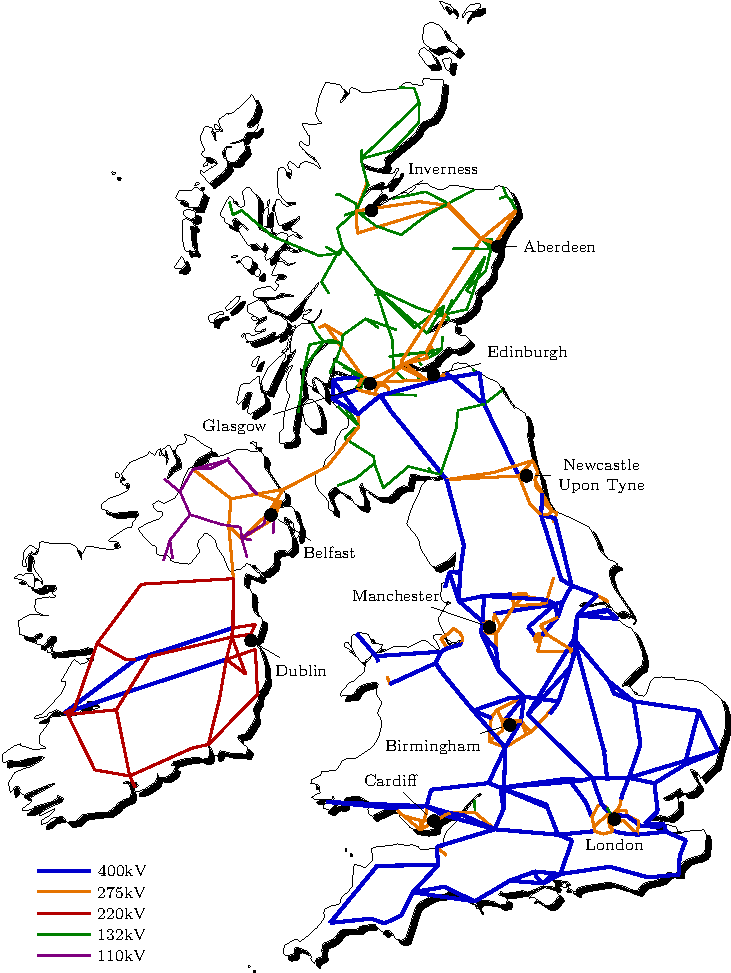
\includegraphics{figures/ngt_grid}
	  \caption{UK transmission system.}
	  \label{fig:ngt_grid}
	\end{figure}
}{}
It is currently too computationally expensive to be solved repeatedly in an
agent-based simulation, but optimisation efforts might allow for it to be used
in studies pertinent to the UK energy industry.

% However, significant improvements in
% speed should be possible through more efficient construction of the Hessian
% matrices in the AC optimal power flow solver.  Agent-based simulation lends
% itself to parallelisation and the artificial neural networks could be
% processed in multiple threads on multi-core processors or on distributed
% memory architectures.

\subsection{AC Optimal Power Flow}
This thesis presents the first application of AC optimal power flow in
electricity market simulation using reinforcement learning agents.  AC optimal
power flow formulations are more difficult to implement and more computationally
expensive to solve than their linearised DC counterparts.  The
additional time and effort required for their use does not always add sufficient
value to simulations.  However, the option to use AC formulations does
provide certain opportunities for further work.

The inclusion of reactive power costs in the objective function of an AC optimal
power flow problem provides an opportunity to run auctions for voltage support
in parallel with those for active power.  These could be open to agents
associated with reactive compensation equipment such as that commonly needed for
wind farm developments.  Traditionally, reactive power markets have been mostly
of academic interest, but as the UK makes greater use of on and off-shore wind
power, the topic could become of increasing importance.

Bus voltages are not all assumed to be 1~per-unit in AC optimal power flow
problems, but are part of the vector of optimisation variables.  Adjusting
phase shift angles, $\theta_{shift}$, can offer a degree of control over
the direction of power flows.  The control of transformer tap ratios, $\tau$,
and phase shift angles by learning agents could become a topic of interest
in congestion management research.

\subsection{Multi-Market Simulation}
% Policy gradient method's superior use of sensory data and their ability to
% operate in large action domains opens opportunities for more detailed study of
% inter-market relationships.
Finally, the global economy is a holistic system of
systems and the analysis of markets independently must be of limited value.
Recent agent-based electricity market studies have investigated the
interaction between electricity, gas and emission allowance markets
\cite{krause:gas,wang:09}.
% Non-linear models [ref] have been published for gas flows in pipelines such as
% those of the UK gas network.

Data for the UK gas transmission network provided by the \citeA{ngtsys2010} is
of limited detail, compared to that for the electricity transmission system,
but suitable models could be used to study the the relationships
between UK gas and electricity markets.  As in \citeA{krause:gas}, actions in
the gas market would constrain the generators options to sell power in subsequent
electricity auctions.  Add to this the option to trade in emissions allowance
markets and agents would be presented with large state and action spaces and
would require suitably advanced learning methods.

% \subsection{Common Information Model}
% Many tools exist for steady-state analysis of balanced three-phase AC networks
% and most are centred around bespoke models that describe the power system
% data.  Several attempts have been made in the past to standardise the format
% in which power system data is stored [CDF, UKGDS, ODF] and latest and most
% popular is the Common Information Model.
%
% The Common Information Model (CIM) is an abstract ontological model that
% describes the elements of national electric power systems and the associations
% between them.  CIM is an evolving international standard approved by the
% International Electrotechnical Commission (IEC).
%
% Unlike many tool specific models the CIM does not simplify the power system
% into a graph of buses connected by branches.  Instead it describes each of the
% components in the system and the electrical connectivity between them.
% Conventional numerical techniques for steady-state analysis of AC power
% systems require a simplified bus-branch model such that when the voltage angle
% and magnitude at each bus is determined the power flows on each branch may be
% calculated.

% market power, constraint management
%\section{Decentralised Trade}
% distribution level, renewables
%\section{Standarisation}
% CIM for markets
%\section{Blackbox optimisation}
% periodic

%\subsection{Summary}

\bibliographystyle{apacite}
\renewcommand{\bibname}{Bibliography}
\bibliography{literature}
%\addcontentsline{toc}{chapter}{Bibliography}

\appendix
\chapter{Open Source Electric Power Engineering Software}
\label{sec:oss}
For the purposes of this thesis the Matlab source code from \matpower was
translated into the Python programming language and released as a project named
Pylon\footnote{http://packages.python.org/Pylon/} \cite{lincoln:pyreto}. It was
translated to allow existing implementations of policy gradient reinforcement
learning methods, from the PyBrain machine learning library \cite{schaul:2010},
to be coupled with \textsc{Matpower}'s scalable and extensible optimal power
flow formulations. With permission from the \matpower developers, the resulting
code was released under the terms of the Apache License, version~2.0, and this
section describes the project in the context of other open source Electrical
Power Engineering software tools to illustrate the contribution made.

Table \ref{tbl:featurematrix} lists the programming language and license
for each of the projects reviewed and shows which projects feature: power
flow (PF), multi-phase power flow (MPF), DC optimal power flow (DCOPF), AC optimal
power flow (ACOPF), continuation power flow (CPF), small-signal stability
analysis (SSSA), time domain simulation (TDS), state estimation (SE), sparse
matrices (SP), a graphical user interface (GUI) and reinforcement learning
(RL) agent based simulation.

%\begin{landscape}
%\begin{table}
\begin{sidewaystable}
%\vspace{1ex}
%\begin{small}
\begin{center}
\begin{tabular}{c|c|c|c|c|c|c|c|c|c|c|c|c|c}
\hline
\textbf{Package} & Language & Licence & PF & MPF & DCOPF & ACOPF & CPF & SSSA &
TDS & SE & SP & GUI & RL \\
\hline
AMES & Java & GPL & & & \stable & & & & & & & \stable & \stable \\
%Cimphony & Java & LGPL & & & & & & & & & \stable & \\
%CIMTool & Java & LGPL & & & & & & & & & \stable & \\
DCOPFJ & Java & GPL & & & \stable & & & & & & & & \\
GridLab-D & \CC & BSD & \stable & \stable & & & & & & & \stable & & \\
MatDyn & \matlab & & & & & & & & \stable & & \stable & & \\
\matpower & \matlab & GPL & \stable & & \stable & \stable & \unstable & & &
\unstable & \stable & & \\
OpenDSS & Pascal & BSD & \stable & \stable & & & & & & & \stable & \stable & \\
PSAT & \matlab & GPL & \stable & & & \stable &
\stable & \stable & \stable & & \stable & \stable & \\
\pylon & Python & Apache & \stable & & \stable & \stable
& & & & \unstable & \stable & \stable & \stable \\
TEFTS & C & & & & & & \stable & & \stable & & \stable & & \\
VST & \matlab & & \stable & & & & \stable & \stable & \stable & & \stable &
\stable & \\
UWPFLOW & C & & & & & & \stable & & & & \stable & & \\
\hline
\end{tabular}
\caption{Open source electric power engineering software feature matrix.}
\label{tbl:featurematrix}
\end{center}
%\end{small}
\end{sidewaystable}
%\end{table}
%\end{landscape}

\section{MATPOWER}
Since 1996, a team of researchers from the Power Systems Engineering Research
Center (PSERC) at Cornell University have been developing \textsc{Matpower}: a
package of Matlab\footnote{Matlab is a registered trademark of The Mathworks,
Inc.} workspace files for solving power flow and optimal power flow problems
\cite{zimmerman:mp_pes}. Initial development was part of the PowerWeb project in
which the team created a power exchange auction market simulator that could be
accessed by multiple users simultaneously through a web-browser interface.
\matpower was originally available under a custom license that permitted use for
any purpose providing the project and authors were cited correctly, but since
version 4.0b3 it has been released under the less permissive \textsc{Gnu}
General Public License (GPL), version 3. \matpower has become very popular in
education and research and has an active mailing list that is moderated by Dr
Ray Zimmerman of PSERC.

\matpower includes five solvers for AC and DC power flow.  The default solver
uses Newton's method \cite{tinney:67} with the full Jacobian matrix updated at
each iteration.  Two variations on the fast decoupled method \cite{stott:74}
described in \citeA{amerongen:89} provide quicker convergence for certain
networks.  The standard Gauss-Seidel method \cite{glimn:57} is provided for
academic purposes and the DC solver provides non-iterative solutions.  The
properties of \matlab sparse matrices are exploited to allow solvers to scale
well with very large systems.  All functions are run from the \matlab
command-line or from within users programs and no graphical user interface is
provided.

Starting with version 4.0, \matpower includes the \matlab Interior Point Solver
(MIPS) that can be used for solving DC and AC optimal power flow problems
\cite{zimmerman:ccv}.  Previously, FMINCON from the \matlab Optimization
Toolbox\footnote{Optimization Toolbox is a registered trademark of The
Mathworks, Inc.} was required or one of a suite of high performance
closed-source solvers:  TSPOPF is a collection of three AC optimal power flow
solvers, implemented in C and released as \matlab MEX files.  It includes the
original implementation of the step-controlled interior point method from which
MIPS was derived.  MINOPF provides an interface to the Fortran based
MINOS\footnote{MINOS is trademark of Stanford Business Software, Inc.} solver,
developed at the Systems Optimization Laboratory at Stanford University, and is
available only for educational and research purposes. Since version 4.0b4
\matpower has also included an interface to IPOPT from the COIN-OR project that
provides an alternative open source solution to MIPS.  DC optimal power flow
problems can be solved with a Quadratic Programming interface to MIPS or using a
MEX interface to BPMPD: a commercial interior point method for linear and
quadratic programming.

\matpower has an extensible optimal power flow formulation that allows users
to introduce additional optimisation variables and problem constraints.  It is
used internally to extend the standard DC and AC formulations to support
piecewise linear cost functions, dispatchable loads, generator PQ capability
curves and branch angle difference limit constraints. Examples of possible
additional extensions include: reserve requirements, environmental costs and
contingency constraints.

\matpower currently runs on Matlab, a
commercial software product from The Mathworks that is supported on all
major platforms, or on \textsc{Gnu}/Octave, a free
program for numerical computation with strong \matlab compatibility.

\section{MATDYN}
\textsc{Matdyn} is an extension to \textsc{Matpower} developed by Stijn Cole
from the Katholieke Universiteit Leuven for dynamic analysis of electric power
systems. It was first released in 2009 under \textsc{Matpower}'s custom license.
It uses the same programming style and extends the \matpower case format with
structs for dynamic generator and event data.  \textsc{Matdyn} uses \matpower to
obtain a power flow solution that is then used in solving a system of
differential algebraic equations representing the power system. Results from
\textsc{Matdyn} have been validated by \citeA{cole:matdyn} against those
obtained from PSS/E\footnote{PSS/E is a registered trademark of Siemens Power
Transmission \& Distribution, Inc.~Power Technologies International.} and the
Power System Analysis Toolbox (See Section \ref{sec:psat}, below) and show good
correspondence.

\section{PSAT}
\label{sec:psat}
The Power System Analysis Toolbox (PSAT) is a \matlab toolbox for static and
dynamic analysis of electric power systems developed by Federico Milano of the
University of Castilla. It is released under the terms of the \textsc{Gnu} GPL
version 2 and offers routines for:
\begin{itemize}
	\item Power flow,
	\item Bifurcation analysis,
	\item Optimal power flow,
	\item Small signal stability analysis,
	\item Time domain simulation and
	\item Phasor measurement unit placement.
\end{itemize}
A large number of input data formats are supported through Perl scripts and
simulation reports can be exported as plain text, Excel spreadsheets or
\LaTeXe~code.  PSAT may be run from the \matlab command-line or through a
\matlab based graphical user interface.  The interface can be used with
Simulink\footnote{Simulink is a registered trademark of The Mathworks, Inc.}
to construct cases such as the UK Generic Distribution System network
shown in Figure \ref{fig:ukgds_ehv3}.  A slightly modified version of PSAT that
can be run from the \textsc{Gnu}/Octave command-line is also available.

\ifthenelse{\boolean{includefigures}}{
%  \begin{landscape}
	\begin{figure}
	  \centering
%	  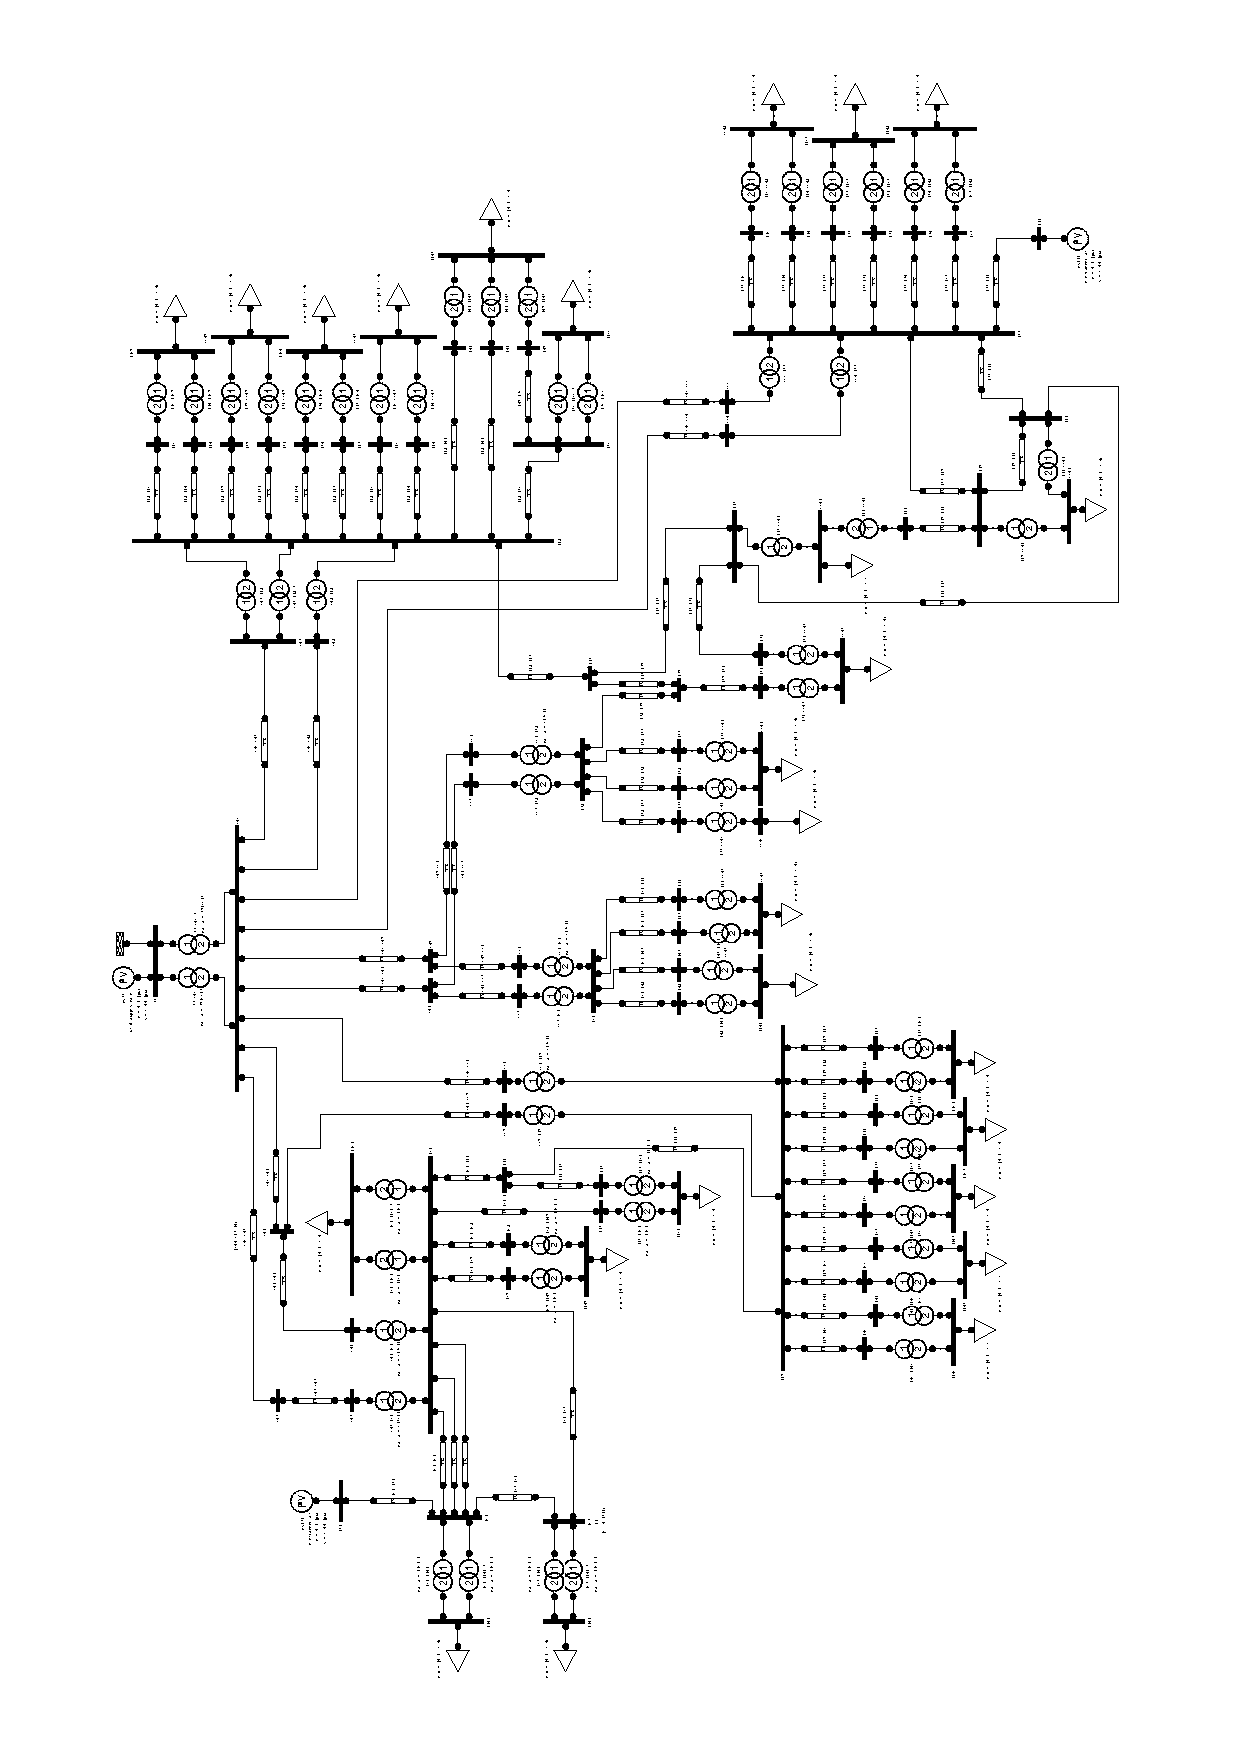
\includegraphics[width=22cm]{figures/psat}
	  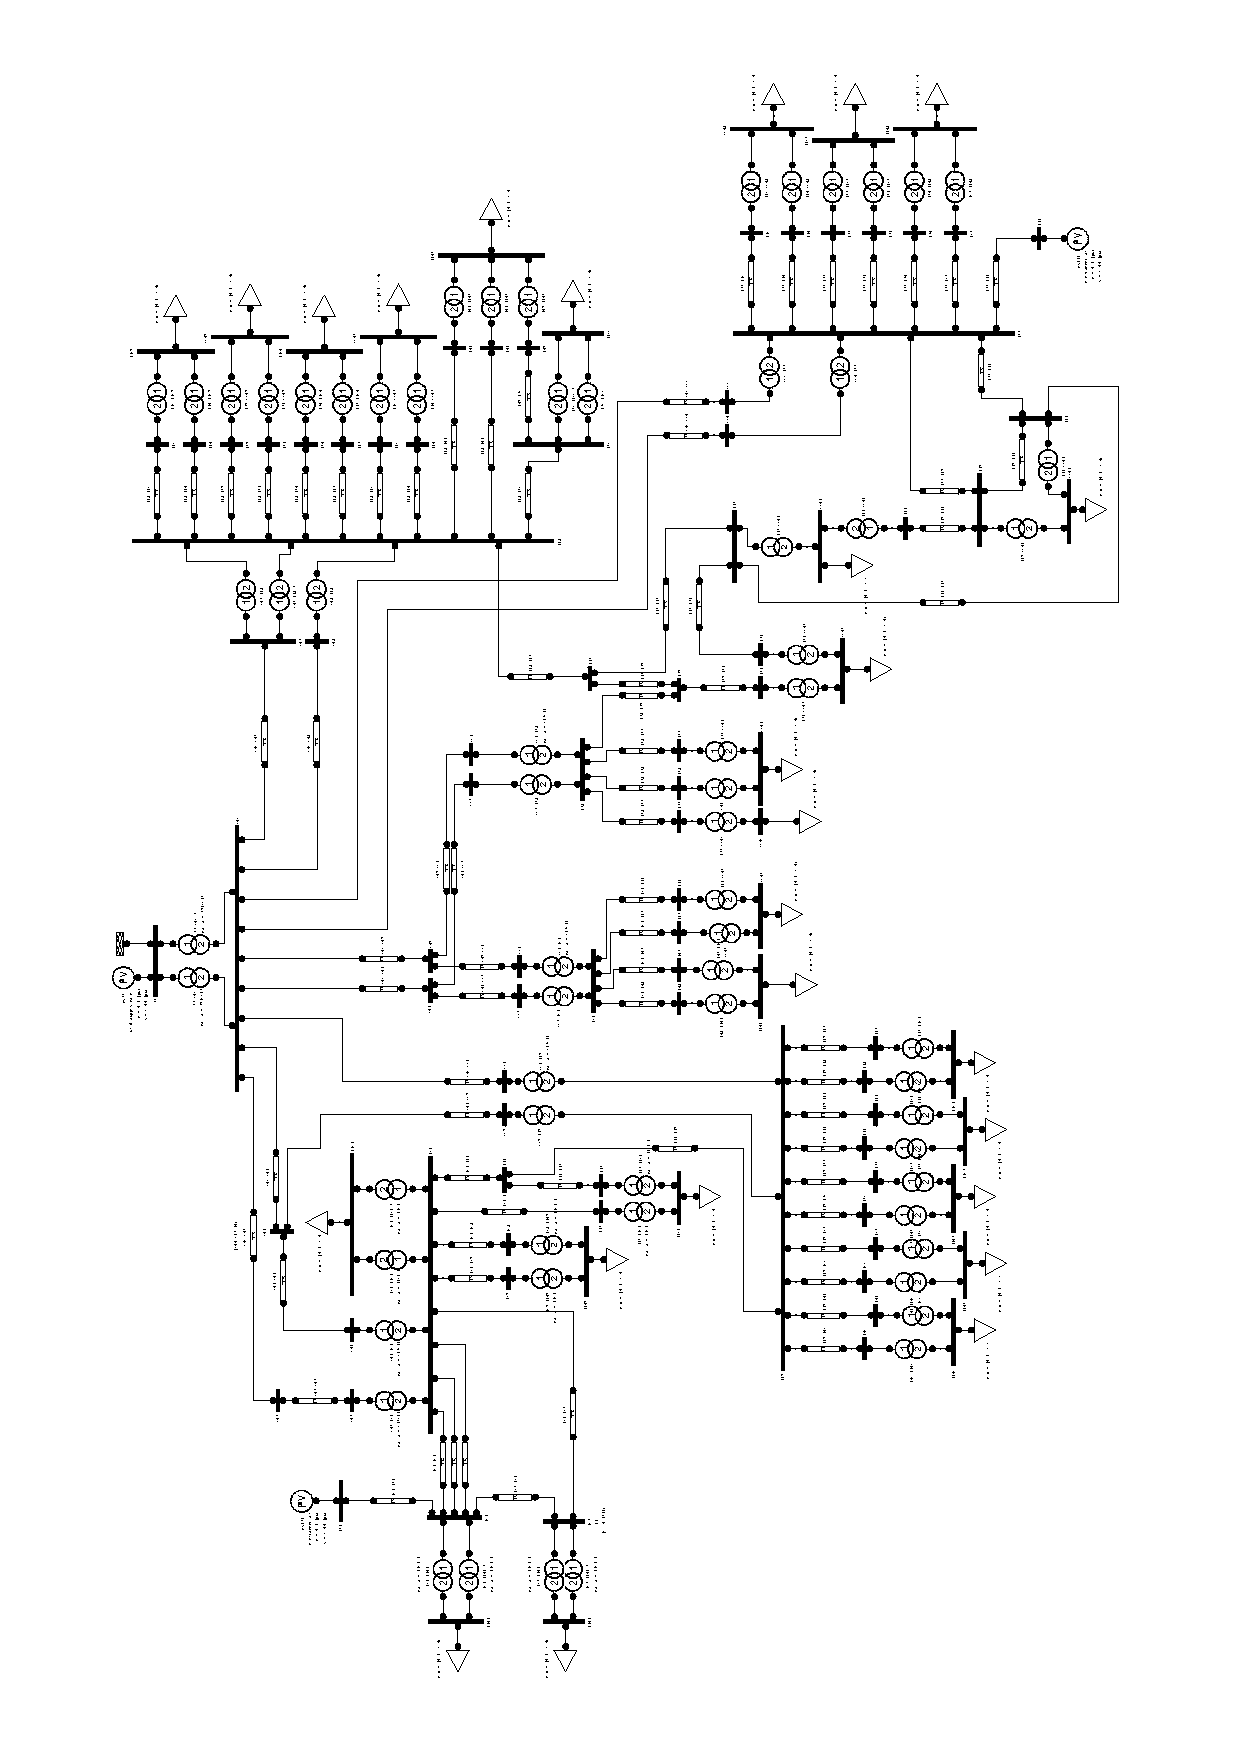
\includegraphics[angle=90,height=22cm]{figures/psat}
	  \caption{UKGDS EHV3 model in PSAT Simulink network editor.}
	  \label{fig:ukgds_ehv3}
	\end{figure}
%  \end{landscape}
}{}

Optimal power flow problems are solved via an interface to the General Algebraic
Modeling System (GAMS).  GAMS defines optimisation problems using a high-level
modelling language and has a large solver portfolio that includes all of the
major commercial and academic solvers.  The interface can be used for solving single
period optimal power flow problems where the objective function can model
maximisation of social benefit, maximisation of the distance to the maximum
loading condition or a multi-objective combination of these. Multi-period
optimal power flow is formulated as a mixed integer problem with linearised
power balance constraints.  The objective function models maximisation of social
welfare, but is extended to include start-up and shutdown costs.

Power flow and dynamic data are often separated in electric power
simulation tools, but in PSAT they are integrated.  This combined with the
large number of routines supported by PSAT can make the code base difficult to
understand and modify.  However, comprehensive documentation is included with
PSAT and the mailing list is very active.
%The majority of correspondance on
%this list concerns PSAT's dynamic simulation features.
The price of GAMS
licenses and the need for optimal power flow problems to be converted to the
GAMS language before being solved may be considered barriers to its
selection for certain projects.

\section{UWPFLOW}
% Continuation and Direct Methods to Locate Fold Bifurcations in AC/DC/FACTS
% Power Systems
UWPFLOW is a research tool for voltage stability analysis developed at the
University of Waterloo, Ontario, and the University of Wisconsin-Madison.  It
is written in ANSI-C and is available as open source for research purposes
only. The program can be run with the terminal command
\begin{center}
\begin{verbatim}
$ uwpflow [-options] input_file
\end{verbatim}
\end{center}
where \texttt{input\_file} is the path to a data file in the IEEE common data
format (CDF) \cite{cdf:73}, that may contain High-Voltage Direct Current (HVDC)
and Flexible Alternating Current Transmission System (FACTS) device data.
Output is also in the CDF and can include additional data for post-processing,
including values for nose curve plots.  An interface to UWPFLOW is provided
with PSAT and can be used for bifurcation analysis.

\section{TEFTS}
% Transient Stability Program to Study Energy Functions and Voltage Stability
% (Bifurcation) Phenomena in AC/DC Power Systems
The University of Waterloo also hosts TEFTS -- a transient stability program
for studying energy functions and voltage stability phenomena in AC/HVDC
dynamic power system models.  It too is written in ANSI-C and is licensed for
research purposes only.  An executable file for DOS is provided and the source
package contains a simple example.

\section{VST}
The Voltage Stability Toolbox (VST) is a \matlab toolbox, developed at the
Center for Electric Power Engineering at Drexel University in Philadelphia, for
investigating stability and bifurcation issues in power systems.  The source
is available for any purpose providing that the authors are suitably cited.
VST features routines for:
\begin{itemize}
  \item Power flow,
  \item Time domain simulation,
  \item Static and dynamic bifurcation analysis,
  \item Singularity analysis and
  \item Eigenvalue analysis.
\end{itemize}
The feature matrix in Table \ref{tbl:featurematrix} shows the similar
capabilities of VST and PSAT. It was developed around the same time and has
the same goals for educational and research applications.  However, VST does
not have the same quality of documentation, graphical user interface or such an
active community of users and developers.

\section{OpenDSS}
In November 2008, the Open Distribution System Simulator (OpenDSS) was released
by the Electric Power Research Institute (EPRI) as open source.  Development of
OpenDSS began in April 1997 and it has been used extensively in studies of
distribution systems including distributed generation impact assessments.
% It is the only open source
% program designed for both distribution and transmission system simulation.

OpenDSS supports steady-state analysis in the frequency domain, including power
flow, harmonics and dynamics.  Arbitrary $n$-phase unbalanced circuit analysis
is supported using an object orientated data model.  Circuit elements are
defined in Object Pascal and solutions are obtained using KLUSolve: a linear
sparse matrix solver written in C and \CC and developed specifically for solving
electrical circuits. The OpenDSS Pascal code is available under the Berkeley
Software Distribution (BSD) license, which allows use for almost any purpose.
KLUSolve, is available under the \textsc{Gnu} Lesser GPL. Circuits are defined
in scripts, using a domain specific language, that may be executed through a
graphical user interface or a Common Object Model (COM) interface. The user
interface also provides circuit data editing, plotting and power flow
visualisation tools.

The power flow solver is fast and can be configured for repeated studies using
daily, yearly or duty-cycle data.  The multi-phase circuit model allows complex
transformer models and fault conditions to be defined and three short-circuit
analysis methods are provided.  The heritage of OpenDSS is in harmonics and
dynamics analysis and it does not support system optimisation.

\section{GridLAB-D}
GridLAB-D is an energy system simulation and analysis tool
designed to investigate the latest energy technologies.  The project was
initiated by the U.S.~Department of Energy in 2004 and developed at Pacific
Northwest National Laboratory.  It was released under a BSD-style license in
September 2009 and has since been developed in collaboration with industry and
academia.

A distributed simulation architecture is used to coordinate energy system
component interactions over short and long timescales.  The core of GridLAB-D is
made up of modules for simulating: distribution and transmission systems,
commercial and residential buildings, energy markets, power system faults and
meteorological systems.  GridLAB-D is written in \CC~and uses a domain specific
language to define models.  Additional modules can be written in \CC~or Java and
Python is under consideration.  It is designed for multicore/multiprocessor
parallelism and the developers intend to use it simulate large areas of the U.S.
on supercomputers.  The source code includes reports and data from the Olympic
Peninsula Project: a futuristic energy pricing experiment that provides a
practical demonstration of GridLAB-D in operation.

GridLAB-D is a unique simulation tool that has the potential to play an
important role in future energy system development.  Its size and complexity
can make for a steep learning curve, but extensive documentation is provided
and training courses are run periodically.  Activity on the mailing lists is low,
suggesting poor uptake, but the software is actively supported and a new
version is under development.

\section{AMES}
\label{sec:ames}
The AMES (Agent-based Modeling of Electricity Systems) power market testbed is
a software package that models core features of the Wholesale Power Market
Platform: a market design proposed by the Federal Energy Regulatory
Commission (FERC) in April 2003 for common adoption in regions of the
U.S.~\cite{tesfatsi:wpmp}. The market design features:
\begin{itemize}
  \item A centralised structure managed by an independent market operator,
  \item Parallel day-ahead and real-time markets and
  \item Locational marginal pricing.
\end{itemize}
Learning agents represent load serving entities or generating companies and
learn using Roth-Erev reinforcement learning methods,
implemented using the Repast agent simulation toolkit \cite{gieseler:thesis}.
% The permissive license under which the source code for
% these algorithms has been released allowed direct translation of them for use
% in this study.
Agents learn from the solutions of hourly bid/offer based
DC-OPF problems formulated as quadratic programs using the DCOPFJ package
\cite{tesfatsi:dcopf} (See Section \ref{sec:dcopfj}, below).

The capabilities of AMES are demonstrated using a 5-bus network model in
\citeA{tesfatsi:pes09}.  The model is provided with AMES and a step-by-step
tutorial describes how it may be used.  AMES comes with a
Swing-based graphical user interface with plotting and table editor tools and
is released under the \textsc{Gnu} GPL, version 2.

\section{DCOPFJ}
\label{sec:dcopfj}
To solve market problems defined in AMES, researchers at Iowa State University
developed a stand-alone DC optimal power flow solver in Java named DCOPFJ.
It formulates optimal power flow problems as convex quadratic programs
which are solved using QuadProgJ.  The same researcher developed QuadProgJ as
an independent solver that uses a dual active set strictly convex quadratic
programming algorithm \cite{goldfarb:scqp}.  DCOPFJ requires
generator costs to be modelled as polynomial functions, of second order or
less, and does not exploit sparse matrix features.

\section{PYLON}
\label{sec:pylon}
% Table \ref{tbl:featurematrix} shows that there are open source software tools
% for all of the main Electric Power Engineering problems and that Matlab is the
% most popular language used.  Several of the projects are more than a decade
% old and the relatively recent release of OpenDSS by EPRI shows that interest
% in this approach to development is not fading.

\pylon is a translation of \matpower v4.0b2 and \textsc{Matdyn} v1.2 to the
Python programming language.  It has extensions for agent-based electricity
market simulation that provide features similar to those of AMES.  Both the DC
and AC formulations of the extensible optimal power flow model from \matpower
are implemented \cite{zimmerman:mp_pes}.  Either a Python version of MIPS or an
interface to IPOPT from COIN-OR can be used to compute solutions.  The sparsity
of the problems is exploited throughout the solution process using matrix
packages from SciPy and bindings to SuperLU or UMFPACK for LU decomposition and
solving sparse sets of linear equations. Scripts are provided for reading and
writing data files in PSS/E, \matpower and PSAT format. A wide variety of
learning methods are available in \pylon due to its use of the PyBrain machine
learning library \cite{schaul:2010}.  PyBrain also provides the artificial
neural network models used for policy function approximation, that may be
accelerated using C extension modules from the ARAC sub-project.

In addition to its market simulation capabilities, \pylon also features solvers
for power flow problems (using fast decoupled or Newton's method), state
estimation, continuation power flow and time domain simulation.  \pylon includes
both a text interface and a graphical user interface (GUI) based on TkInter:
which is included with Python and imposes no additional dependencies.  A feature
rich GUI is provided by plug-ins for Puddle: an extensible, GUI toolkit
independent integrated development environment, developed for the purposes of
this thesis also.

The use of matrix
libraries from NumPy and SciPy has allowed \pylon (with the permission of the
\matpower developers) to be released under the Apache license, version 2.0. This
allows \pylon to be used as a library in proprietary software as well as
free and open source tools since derivatives of the source code may be made
available under more restrictive terms than the original Apache license.  This
is in contrast to strong ``copyleft'' licenses, such as the \textsc{Gnu} GPL,
that require the same rights to be preserved in modified versions of the work.

\section*{Summary}
A diverse range of open source Electric Power Engineering tools are available.
Implementations of most of the traditional power system analysis routines can be
found and many offer performance comparable with proprietary offerings.  Various
programming languages are used, but Matlab is the most popular choice.

Several projects are licensed under the \textsc{Gnu} GPL and it ensures that all
users have access to the full source code.  This does impose restrictions on the
redistribution of projects that use the routines and this can be a barrier to
use in certain types of project.  To encourage commercial use and promote
industrial involvement, two large code bases (OpenDSS and GridLAB-D) have
recently been released under weak copyleft licenses.  Pylon was developed using
specific scientific computing libraries and permission was obtained from the
developers of \matpower to allow release under a similarly permissive license.
Most of the projects described above are led and developed by one individual
and contributions from the user community are typically minimal.  It is hoped
that Pylon's use of a popular free programming language and its liberal
licensing conditions will encourage community involvement and lead to inventive
combinations of simulation routines and web technologies in the
development of intelligent electric power grids.

\chapter{Case Data}
This appendix provides data for the electric power system models used in
Chapters \ref{ch:nashanalysis} and \ref{ch:exploitation}.

\section{6-Bus Case}
\label{adx:case6ww}
The data for the six bus case adapted from \citeA[pp.~104, 112, 119, 123-124,
549]{wood:pgoc} is presented in this section.  The data was imported from the
``case6ww.m'' case file provided with \textsc{Matpower}.
% Figure \ref{fig:case6ww2} illustrates the structure of the model and shows the
% bus injections for the AC unit de-commitment optimal power flow solution.
Table \ref{tbl:case6ww_bus} lists the bus data, Table \ref{tbl:case6ww_gen}
lists the generator data and Table \ref{tbl:case6ww_branch} lists the branch
data.

%\ifthenelse{\boolean{includefigures}}{\begin{figure}
\label{fig:case6ww}
\centering
\begin{scriptsize}
\begin{tikzpicture}[thick]

\coordinate (c1) at (0,4);
\coordinate (c2) at (5,6.5);
\coordinate (c3) at (10,4);
\coordinate (c4) at (0,0);
\coordinate (c5) at (5,-2.5);
\coordinate (c6) at (10,0);
\coordinate (over) at (0,3.75);

\busbar{b1}{c1}{20mm}
\busbar{b2}{c2}{30mm}
\busbar{b3}{c3}{20mm}
\busbar{b4}{c4}{20mm}
\busbar{b5}{c5}{30mm}
\busbar{b6}{c6}{20mm}

% Branch 1-2.
\draw[line] ([xshift=5mm] b1.north) node[rotate=90,above right]{$15.41$}
node[rotate=90,below right]{$-9.58$} -- ++(0,3.75) -| ([xshift=-8mm] b2.north)
node[rotate=90,above right]{$-15.14$} node[rotate=90,below right]{$5.70$};
% Branch 1-4.
\draw[line] ([xshift=-5mm] b1.south) node[rotate=90,above left]{$33.95$}
node[rotate=90,below left]{$22.50$} -- ([xshift=-5mm] b4.north)
node[rotate=90,above right]{$-33.15$} node[rotate=90,below right]{$-23.46$};
% Branch 1-5.
\draw[line] ([xshift=5mm] b1.south) node[rotate=90,above left]{$27.86$}
node[rotate=90,below left]{$12.80$} -- ([xshift=5mm,yshift=-15mm] b1.south)
-- ([xshift=-8mm,yshift=15mm] b5.north) -- ([xshift=-8mm] b5.north)
node[rotate=90,above right]{$-27.11$} node[rotate=90,below right]{$-16.20$};
% Branch 2-3.
\draw[line] ([xshift=8mm] b2.north) node[rotate=90,above right]{$0.29$}
node[rotate=90,below right]{$-11.76$} -- ++(0,1.25) -| ([xshift=-5mm] b3.north)
node[rotate=90,above right]{$-0.25$} node[rotate=90,below right]{$5.18$};
% Branch 2-4.
\draw[line,ultra thick] ([xshift=-8mm] b2.south) node[rotate=90,above
left]{$41.74$} node[rotate=90,below left]{$43.11$} --
([xshift=-8mm,yshift=-15mm] b2.south) -- node[sloped,above]{$\vert S_{max}^5
\vert = 60.0$} ([xshift=5mm,yshift=15mm] b4.north) -- ([xshift=5mm] b4.north)
node[rotate=90,above right]{$-40.06$} node[rotate=90,below right]{$-41.83$};
% Branch 2-5.
\draw[line] (b2.south) node[rotate=90,above left]{$17.35$}
node[rotate=90,below left]{$14.93$} -- (b5.north) node[rotate=90,above
right]{$-16.81$} node[rotate=90,below right]{$-17.46$};
% Branch 2-6.
\draw[line] ([xshift=8mm] b2.south) node[rotate=90,above left]{$25.03$}
node[rotate=90,below left]{$12.67$} -- ([xshift=8mm,yshift=-15mm] b2.south)
-- ([xshift=-5mm,yshift=15mm] b6.north) -- ([xshift=-5mm] b6.north)
node[rotate=90,above right]{$-24.49$} node[rotate=90,below right]{$-16.38$};
% Branch 3-5.
\draw[line] ([xshift=-5mm] b3.south) node[rotate=90,above left]{$23.18$}
node[rotate=90,below left]{$21.57$} -- ([xshift=-5mm,yshift=-15mm] b3.south)
-- ([xshift=8mm,yshift=15mm] b5.north) -- ([xshift=8mm] b5.north)
node[rotate=90,above right]{$-21.99$} node[rotate=90,below right]{$-24.28$};
% Branch 3-6.
\draw[line] ([xshift=5mm] b3.south) node[rotate=90,above left]{$47.50$}
node[rotate=90,below left]{$59.90$} -- ([xshift=5mm] b6.north)
node[rotate=90,above right]{$-46.45$} node[rotate=90,below right]{$-56.82$};
% Branch 4-5.
\draw[line] ([xshift=5mm] b4.south) node[rotate=90,above left]{$3.21$}
node[rotate=90,below left]{$-4.71$} -- ++(0,-3.75) -| ([xshift=-8mm] b5.south)
node[rotate=90,above left]{$-3.19$} node[rotate=90,below left]{$-3.03$};
% Branch 5-6.
\draw[line] ([xshift=8mm] b5.south) node[rotate=90,above left]{$-0.90$}
node[rotate=90,below left]{$-9.03$} -- ++(0,-1.25) -| ([xshift=-5mm] b6.south)
node[rotate=90,above left]{$0.94$} node[rotate=90,below left]{$3.21$};

% Generator 1.
\genset{g1}{$(c1)+(-5mm,15mm)$}
\draw[line] ([xshift=-5mm] b1.north) -- node[sloped,above]{$77.22$}
node[sloped,below]{$25.72$} (g1.south);
% Generator 2.
\genset{g2}{$(c2)+(0,15mm)$}
\draw[line] (b2.north) -- node[sloped,above]{$69.27$}
node[sloped,below]{$64.65$} (g2.south);
% Generator 3.
\genset{g3}{$(c3)+(5mm,15mm)$}
\draw[line] ([xshift=5mm] b3.north) -- node[sloped,above]{$70.42$}
node[sloped,below]{$86.64$} (g3.south);

% Load 1.
\loadd{l1}{$(c4)-(5mm,15mm)$}
\draw[line] (l1.south) -- node[sloped,above]{$70.00$}
node[sloped,below]{$70.00$} ([xshift=-5mm] b4.south);
% Load 2.
\loadd{l2}{$(c5)-(0mm,15mm)$}
\draw[line] (l2.south) -- node[sloped,above]{$70.00$}
node[sloped,below]{$70.00$} (b5.south);
% Load 3.
\loadd{l3}{$(c6)+(5mm,-15mm)$}
\draw[line] (l3.south) -- node[sloped,above]{$70.00$}
node[sloped,below]{$70.00$} ([xshift=5mm] b6.south);

\end{tikzpicture}
\end{scriptsize}
\caption{One line diagram for six bus power system model from [].}
\end{figure}
}{}
%\ifthenelse{\boolean{includefigures}}{\input{tikz/case6ww2}}{}

\begin{table}[h]
\caption{6-bus case bus data.}
\label{tbl:case6ww_bus}
\begin{center}
\begin{tabular}{c|c|c|c|c|c|c|c}
\hline
Bus &$p_d$ &$q_d$ &$g_s$ &$b_s$ &$v_{base}$ &$v_{max}$ &$v_{min}$\\
\hline\hline
%%%%%%%%%%%%%%%%%%%%%%%%%%%%%%%%%%%%%%%%%%%%%%%%%%%%%%%%%%%%%%%%%%%%%%
%%                                                                  %%
%%  This is a LaTeX2e table fragment exported from Gnumeric.        %%
%%                                                                  %%
%%%%%%%%%%%%%%%%%%%%%%%%%%%%%%%%%%%%%%%%%%%%%%%%%%%%%%%%%%%%%%%%%%%%%%
1	&0	&0	&0	&0	&230	&1.05	&1.05\\
2	&0	&0	&0	&0	&230	&1.05	&1.05\\
3	&0	&0	&0	&0	&230	&1.07	&1.07\\
4	&70	&70	&0	&0	&230	&1.05	&0.95\\
5	&70	&70	&0	&0	&230	&1.05	&0.95\\
6	&70	&70	&0	&0	&230	&1.05	&0.95\\

\hline
\end{tabular}
\end{center}
\end{table}

\begin{table}[h]
\caption{6-bus case generator data.}
\label{tbl:case6ww_gen}
\begin{center}
\begin{tabular}{c|c|c|c|c|c}
\hline
Bus &$p_{max}$ &$p_{min}$ &$v_g$ &$q_{max}$ &$q_{min}$\\
\hline\hline
%%%%%%%%%%%%%%%%%%%%%%%%%%%%%%%%%%%%%%%%%%%%%%%%%%%%%%%%%%%%%%%%%%%%%%
%%                                                                  %%
%%  This is a LaTeX2e table fragment exported from Gnumeric.        %%
%%                                                                  %%
%%%%%%%%%%%%%%%%%%%%%%%%%%%%%%%%%%%%%%%%%%%%%%%%%%%%%%%%%%%%%%%%%%%%%%
1	&1.05	&200	&50	&100	&-100\\
2	&1.05	&150	&37.5	&100	&-100\\
3	&1.07	&180	&45	&100	&-100\\

\hline
\end{tabular}
\end{center}
\end{table}

\begin{table}[h]
\caption{6-bus case branch data.}
\label{tbl:case6ww_branch}
\begin{center}
\begin{tabular}{c|c|c|c|c|c|c|c}
\hline
From &To &$r$ &$x$ &$b_c$ &$s_{max}$ &$\tau$ &$\theta_{shift}$\\
\hline\hline
%%%%%%%%%%%%%%%%%%%%%%%%%%%%%%%%%%%%%%%%%%%%%%%%%%%%%%%%%%%%%%%%%%%%%%
%%                                                                  %%
%%  This is a LaTeX2e table fragment exported from Gnumeric.        %%
%%                                                                  %%
%%%%%%%%%%%%%%%%%%%%%%%%%%%%%%%%%%%%%%%%%%%%%%%%%%%%%%%%%%%%%%%%%%%%%%
1	&2	&0.1	&0.2	&0.04	&40	&0	&0\\
1	&4	&0.05	&0.2	&0.04	&60	&0	&0\\
1	&5	&0.08	&0.3	&0.06	&40	&0	&0\\
2	&3	&0.05	&0.25	&0.06	&40	&0	&0\\
2	&4	&0.05	&0.1	&0.02	&60	&0	&0\\
2	&5	&0.1	&0.3	&0.04	&30	&0	&0\\
2	&6	&0.07	&0.2	&0.05	&90	&0	&0\\
3	&5	&0.12	&0.26	&0.05	&70	&0	&0\\
3	&6	&0.02	&0.1	&0.02	&80	&0	&0\\
4	&5	&0.2	&0.4	&0.08	&20	&0	&0\\
5	&6	&0.1	&0.3	&0.06	&40	&0	&0\\

\hline
\end{tabular}
\end{center}
\end{table}

\section{IEEE Reliability Test System}
\label{adx:ieee_rts}
This section provides data for the modified IEEE Reliability Test System that
was imported from the ``case24\_ieee\_rts.m'' case file, provided with \matpower
and was originally contributed by Bruce Wollenberg.
Table \ref{tbl:rtsbus} lists the bus data, Table \ref{tbl:rtsgen} lists the
generator data and Table \ref{tbl:rtsbranch} lists the branch data.
% Table \ref{tbl:rtsgencost} lists the generator cost data provided by Georgia
% Tech Power Systems Control and Automation Laboratory.

%\ifthenelse{\boolean{includefigures}}{\newcommand{\generatorunit}[3]{
  \node[circle,draw,thick,minimum width=6mm,#3] (#1) at (#2) {};
  \draw[thick] ($(#2)-(2mm,0)$) sin ++(1mm,1mm) cos ++(1mm,-1mm)
  sin ++(1mm,-1mm) cos ++(1mm,1mm);
}

\begin{figure}
\centering
\small
\begin{tikzpicture}[thick,label distance=0mm]
  \tikzstyle{busbar} = [rectangle,draw,fill=black!50,inner sep=0pt];
  \tikzstyle{hbus} = [busbar,minimum width=10mm,minimum height=2pt];
  \tikzstyle{vbus} = [busbar,minimum width=2pt,minimum height=10mm];
  \tikzstyle{overhead} = [-,thick];
  \tikzstyle{cable} = [thick];
  \tikzstyle{trxcircle} = [circle,draw=black,inner sep=0pt,minimum width=5mm];
  \tikzstyle{every pin edge}=[-,shorten <=1pt,thin];

\node[hbus,minimum width=15mm,label=left:Bus 1] (bus1) at (5,0) {};
\node[hbus,minimum width=15mm,label=right:Bus 2] (bus2) at (7,0) {};
\node[hbus,label=right:Bus 3] (bus3) at (0,6) {};
\node[vbus,label=above:Bus 4] (bus4) at (3,4) {};
\node[vbus,label=above:Bus 5] (bus5) at (6.5,3) {};
\node[vbus,label=above:Bus 6] (bus6) at (12,5.3) {};
\node[hbus,label=right:Bus 7] (bus7) at (11,0.5) {};
\node[vbus,label=above:Bus 8] (bus8) at (12,3) {};
\node[hbus,minimum width=20mm,label=left:Bus 9] (bus9) at (5,6) {};
\node[hbus,minimum width=20mm,label=right:Bus 10] (bus10) at (8,6) {};
\node[hbus,minimum width=20mm,label=left:Bus 11] (bus11) at (5,8) {};
\node[hbus,minimum width=20mm,label=right:Bus 12] (bus12) at (8,8) {};
\node[vbus,label={[xshift=-4mm]below:Bus 13}] (bus13) at (12,10) {};
\node[vbus,label=above:Bus 14] (bus14) at (3.5,11.5) {};
\node[hbus,minimum width=20mm,label=right:Bus 15] (bus15) at (0.5,12) {};
\node[hbus,minimum width=15mm,label=right:Bus 16] (bus16) at (0,14) {};
\node[vbus,minimum height=20mm,label=above:Bus 17] (bus17) at (-1,16) {};
\node[hbus,minimum width=20mm,label=right:Bus 18] (bus18) at (2,18) {};
\node[hbus,label=below right:Bus 19] (bus19) at (4.5,14) {};
\node[hbus,minimum width=15mm,label=below right:Bus 20] (bus20) at (7,14) {};
\node[hbus,minimum width=25mm,label=right:Bus 21] (bus21) at (5,17) {};
\node[hbus,label=right:Bus 22] (bus22) at (9,17) {};
\node[vbus,minimum height=15mm,label=above:Bus 23] (bus23) at (11,14.55) {};
\node[hbus,label=right:Bus 24] (bus24) at (0,8) {};

% Branch 1-2.
\draw[cable] ([xshift=5mm] bus1.north) -- ++(0,5mm) node[xshift=5mm,above]
{cable} -| ([xshift=-5mm] bus2.north);
% Branch 1-3.
\draw[overhead] ([xshift=-5mm] bus1.north) -- ([xshift=-5mm,yshift=5mm]
bus1.north) -- ([xshift=0mm,yshift=-5mm] bus3.south) -- (bus3.south);
% Branch 1-5.
\draw[overhead] (bus1.north) |- (bus5.west);
% Branch 2-4.
\draw[overhead] (bus2.north) -- ([yshift=5mm] bus2.north) -- ([xshift=5mm]
bus4.east) -- (bus4.east);
% Branch 2-6.
\draw[overhead] ([xshift=5mm] bus2.north) -- ([xshift=5mm,yshift=5mm]
bus2.north) -- ([xshift=-5mm,yshift=-3mm] bus6.west) -- ([yshift=-3mm]
bus6.west);
% Branche 3-9.
\draw[overhead] ([xshift=3mm] bus3.south) -- ++(0,-5mm) -| ([xshift=-5mm]
bus9.south);
% Branch 3-24.
\draw node[trxcircle,yshift=-1mm,above of=bus3] (t3-24p) {};
\draw node[trxcircle,yshift=1mm,above of=bus3] (t3-24s) {};
\draw[overhead] (bus3.north) -- (t3-24p.south);
\draw[overhead] (t3-24s.north) -- (bus24.south);
% Branch 4-9.
\draw[overhead] ([yshift=3mm] bus4.east) -- ([xshift=5mm,yshift=3mm] bus4.east)
-- ([yshift=-5mm] bus9.south) -- (bus9.south);
% Branch 5-10.
\draw[overhead] (bus5.east) -| (bus10.south);
% Branch 6-10.
\draw[overhead] (bus6.west) -| node[above right] {cable} ([xshift=5mm]
bus10.south);
% Branch 7-8.
\draw[overhead] ([xshift=-3mm] bus7.north) |- ([yshift=-3mm] bus8.west);
% Branch 8-9.
\draw[overhead] (bus8.west) -- ([xshift=-5mm] bus8.west) --
([xshift=5mm,yshift=-5mm] bus9.south) -- ([xshift=5mm] bus9.south);
% Branch 8-10;
\draw[overhead] ([yshift=3mm] bus8.west) -- ([xshift=-5mm,yshift=3mm]
bus8.west) -- ([xshift=-5mm,yshift=-10mm] bus10.south) -- ([xshift=-5mm]
bus10.south);
% Branch 9-11.
\draw node[trxcircle,yshift=-1mm,xshift=-5mm,above of=bus9] (t9-11p) {};
\draw node[trxcircle,yshift=1mm,xshift=-5mm,above of=bus9] (t9-11s) {};
\draw[overhead] ([xshift=-5mm] bus9.north) -- (t9-11p.south);
\draw[overhead] (t9-11s.north) -- ([xshift=-5mm] bus11.south);
% Branch 9-12.
\draw node[trxcircle,yshift=-1mm,xshift=-5mm,node distance=7mm,below of=bus12]
(t9-12p) {};
\draw node[trxcircle,yshift=1mm,xshift=-5mm,node distance=7mm,below of=bus12]
(t9-12s) {};
\draw[overhead] ([xshift=5mm] bus9.north) -- ([xshift=5mm,yshift=3mm]
bus9.north) -- ([yshift=-3mm] t9-12p.south) -- (t9-12p.south);
\draw[overhead] (t9-12s.north) -- ([xshift=-5mm] bus12.south);
% Branch 10-11.
\draw node[trxcircle,yshift=-1mm,xshift=5mm,node distance=7mm,below of=bus11]
(t10-11p) {};
\draw node[trxcircle,yshift=1mm,xshift=5mm,node distance=7mm,below of=bus11]
(t10-11s) {};
\draw[overhead] ([xshift=-5mm] bus10.north) -- ([xshift=-5mm,yshift=3mm]
bus10.north) -- ([yshift=-3mm] t10-11p.south) -- (t10-11p.south);
\draw[overhead] (t10-11s.north) -- ([xshift=5mm] bus11.south);
% Branch 10-12.
\draw node[trxcircle,yshift=-1mm,xshift=5mm,above of=bus10] (t10-12p) {};
\draw node[trxcircle,yshift=1mm,xshift=5mm,above of=bus10] (t10-12s) {};
\draw[overhead] ([xshift=5mm] bus10.north) -- (t10-12p.south);
\draw[overhead] (t10-12s.north) -- ([xshift=5mm] bus12.south);
% Branch 11-13.
\draw[overhead] ([xshift=5mm] bus11.north) -- ([xshift=5mm,yshift=5mm]
bus11.north) -- ([xshift=-5mm] bus13.west) -- (bus13.west);
% Branch 11-14.
\draw[overhead] ([xshift=-5mm] bus11.north) |- ([yshift=-3mm] bus14.east);
% Branch 12-13.
\draw[overhead] ([xshift=-5mm] bus12.north) -- ([xshift=-5mm,yshift=7mm]
bus12.north) -- ([xshift=-5mm,yshift=-3mm] bus13.west) -- ([yshift=-3mm]
bus13.west);
% Branch 12-23.
\draw[overhead] ([xshift=5mm] bus12.north) |- ([yshift=-5mm] bus23.west);
% Branch 13-23.
\draw[overhead] ([yshift=3mm] bus13.west) -- ([xshift=-5mm,yshift=3mm]
bus13.west) |- ([yshift=-5mm] bus23.east);
% Branch 14-16.
\draw[overhead] ([yshift=3mm] bus14.west) -- ([xshift=-6mm,yshift=3mm]
bus14.west) |- ([xshift=5mm,yshift=-5mm] bus16.south) -- ([xshift=5mm]
bus16.south);
% Branch 15-16.
\draw[overhead] ([xshift=-5mm] bus15.north) -- (bus16.south);
% Branches 15-21.
\draw[overhead] (bus15.north) -- ([yshift=5mm] bus15.north) -- ([yshift=-10mm]
bus21.south) -- (bus21.south);
\draw[overhead] ([xshift=5mm] bus15.north) -- ([xshift=5mm,yshift=5mm]
bus15.north) -- ([xshift=5mm,yshift=-10mm] bus21.south) -- ([xshift=5mm]
bus21.south);
% Branch 15-24.
\draw[overhead] ([xshift=-5mm] bus15.south) -- (bus24.north);
% Branch 16-17.
\draw[overhead] ([xshift=-5mm] bus16.north) |- ([yshift=-5mm] bus17.east);
% Branch16-19.
\draw[overhead] ([xshift=5mm] bus16.north) -- ([xshift=5mm,yshift=5mm]
bus16.north) -| ([xshift=-3mm] bus19.north);
% Branch 17-18.
\draw[overhead] ([yshift=5mm] bus17.east) -| ([xshift=-5mm] bus18.south);
% Branch 17-22.
\draw[overhead] (bus17.east) -- ([xshift=20mm] bus17.east) -- ([xshift=20mm,
yshift=-5mm] bus17.east) -| ([xshift=3mm] bus22.south);
% Branches 18-21.
\draw[overhead] (bus18.south) -- ([yshift=-20mm] bus18.south) -|
([xshift=-5mm] bus21.south);
\draw[overhead] ([xshift=5mm] bus18.south) -- ([xshift=5mm,yshift=-15mm]
bus18.south) -| ([xshift=-10mm] bus21.south);
% Branches 19-20.
\draw[overhead] (bus19.north) -- ([yshift=10mm] bus19.north) -|
([xshift=-1.5mm] bus20.north);
\draw[overhead] ([xshift=3mm] bus19.north) -- ([xshift=3mm,yshift=5mm]
bus19.north) -| ([xshift=-4.5mm] bus20.north);
% Branches 20-23.
\draw[overhead] ([xshift=1.5mm] bus20.north) |- ([yshift=5mm] bus23.west);
\draw[overhead] ([xshift=4.5mm] bus20.north) |- (bus23.west);
% Branch 21-22.
\draw[overhead] ([xshift=10mm] bus21.south) -- ([xshift=10mm,yshift=-7.5mm]
bus21.south) -| ([xshift=-3mm] bus22.south);

% Generator @ Bus 1.
\generatorunit{gen1}{4.5,-0.8}{label=left:192 MW,pin={[pin distance=12mm,text
centered,text width=10.5mm]165:2$\times$U20 2$\times$U76}};
\draw[overhead] ([xshift=-5mm] bus1.south) -- (gen1.north);
% Generator @ Bus 2.
\generatorunit{gen2}{7.5,-0.8}{label=right:192 MW,pin={[pin distance=12mm,text
centered,text width=10.5mm]15:2$\times$U20 2$\times$U76}};
\draw[overhead] ([xshift=5mm] bus2.south) -- (gen2.north);
% Generator @ Bus 7.
\generatorunit{gen3}{11,-0.3}{label=right:300 MW,pin=below:3$\times$U100};
\draw[overhead] (bus7.south) -- (gen3.north);
% Generator @ Bus 13.
\generatorunit{gen4}{12.3,10.9}{label=above:591 MW,pin={[pin distance=8mm]
left:3$\times$U197}};
\draw[overhead] ([yshift=3mm] bus13.east) -- ([yshift=3mm,xshift=2.5mm]
bus13.east) -- (gen4.south);
% Generator @ Bus 14.
\generatorunit{gen5}{4.3,11.8}{label={[text justified,text
width=15mm]right:Synch. Cond.}}; \draw[overhead] ([yshift=3mm] bus14.east) --
(gen5.west);
% Generator @ Bus 15.
\generatorunit{gen6}{0.5,11.2}{label={[text centered,text width=10mm]below:215 MW},
pin={[pin distance=5mm,text centered,text width=15mm]-70:5$\times$U12
1$\times$U155}}; \draw[overhead] (bus15.south) -- (gen6.north);
% Generator @ Bus 16.
\generatorunit{gen7}{0.0,15}{label=right:155 MW};
\draw[overhead] (bus16.north) -- (gen7.south);
% Generator @ Bus 18.
\generatorunit{gen8}{1.5,18.8}{label=left:400 MW,pin={[pin distance=6mm]below
left:Nuclear}}; \draw[overhead] ([xshift=-5mm] bus18.north) -- (gen8.south);
% Generator @ Bus 21.
\generatorunit{gen9}{5,17.8}{label=right:400 MW,pin={above right:Nuclear}};
\draw[overhead] (bus21.north) -- (gen9.south);
% Generator @ Bus 22.
\generatorunit{gen10}{9,17.8}{label=right:300 MW,pin={above:Hydro, 6$\times$U50}};
\draw[overhead] (bus22.north) -- (gen10.south);
% Generator @ Bus 23.
\generatorunit{gen11}{11.8,15.05}{label=below:660 MW,pin={[text centered,text
width=15mm]above:2$\times$U155 1$\times$U350}};
\draw[overhead] ([yshift=5.05mm] bus23.east) -- (gen11.west);

% Load @ Bus 1.
\draw[loadline] ([xshift=5mm] bus1.south) -- ++(0,-0.8) node[text centered,text
width=10mm,below] {108 MW};
% Load @ Bus 2.
\draw[loadline] ([xshift=-5mm] bus2.south) -- ++(0,-0.8) node[text
centered,text width=10mm,below] {97 MW};
% Load @ Bus 3.
\draw[loadline] ([xshift=-3mm] bus3.south) -- ++(0,-0.8) node[text
centered,text width=10mm,below] {108 MW};
% Load @ Bus 4.
\draw[loadline] ([yshift=-3mm] bus4.east) -- ++(3mm,0) -- ++(0,-0.8)
node[below] {74 MW};
% Load @ Bus 5.
\draw[loadline] ([yshift=-3mm] bus5.east) -- ++(3mm,0) --
++(0,-0.8) node[below] {71 MW};
% Load @ Bus 6.
\draw[loadline] (bus6.east) -- ++(3mm,0) -- ++(0,-0.8) node[below] {136 MW};
% Load @ Bus 7.
\draw[loadline] ([xshift=3mm] bus7.north) -- ++(0,0.8) node[right] {125 MW};
% Load @ Bus 8.
\draw[loadline] (bus8.east) -- ++(3mm,0) -- ++(0,-0.8) node[left] {171 MW};
% Load @ Bus 9.
\draw[loadline] ([xshift=2.5mm] bus9.south) -- ++(0,-1) node[below] {175 MW};
% Load @ Bus 10.
\draw[loadline] ([xshift=7.5mm] bus10.north) -- ++(0,3mm) -- ++(8mm,0)
node[above right] {195 MW};
% Load @ Bus 13.
\draw[loadline] ([yshift=-3mm] bus13.east) -- ++(2.5mm,0) -- ++(0,-1)
node[below] {265 MW};
% Load @ Bus 14.
\draw[loadline] ([yshift=-3mm] bus14.west) -- ++(-3mm,0) -- ++(0,-0.8)
node[below] {194 MW};
% Load @ Bus 15.
\draw[loadline] ([xshift=7mm] bus15.south) -- ++(0,-0.8) node[right]
{317 MW};
% Load @ Bus 16.
\draw[loadline] ([xshift=-5mm] bus16.south) -- ++(0,-0.8) node[text centered,
text width=10mm,below] {100 MW};
% Load @ Bus 18.
\draw[loadline] ([xshift=5mm] bus18.north) -- ++(0,0.8) node[right] {333 MW};
% Load @ Bus 19.
\draw[loadline] (bus19.south) -- ++(0,-0.8) node[right] {181 MW};
% Load @ Bus 20.
\draw[loadline] (bus20.south) -- ++(0,-0.8) node[below] {128 MW};

% Area voltage labels.
\node[draw] at (1,2) {\normalsize{138 kV}};
\node[draw] at (6.5,10.3) {\normalsize{230 kV}};

\end{tikzpicture}
\caption{IEEE Reliability Test System}
\label{fig:ieee79rts}
\end{figure}}{}
%\ifthenelse{\boolean{includefigures}}{\input{tikz/ieee79rts2}}{}

\begin{table}[h]
\caption{IEEE RTS bus data.}
\label{tbl:rtsbus}
\begin{center}
\begin{tabular}{c|c|c|c|c|c|c|c}
\hline
Bus &$p_d$ &$q_d$ &$g_s$ &$b_s$ &$v_{base}$ &$v_{max}$ &$v_{min}$\\
\hline\hline
%%%%%%%%%%%%%%%%%%%%%%%%%%%%%%%%%%%%%%%%%%%%%%%%%%%%%%%%%%%%%%%%%%%%%%
%%                                                                  %%
%%  This is a LaTeX2e table fragment exported from Gnumeric.        %%
%%                                                                  %%
%%%%%%%%%%%%%%%%%%%%%%%%%%%%%%%%%%%%%%%%%%%%%%%%%%%%%%%%%%%%%%%%%%%%%%
1	&108	&22	&0	&0	&138	&1.05	&0.95\\
2	&97	&20	&0	&0	&138	&1.05	&0.95\\
3	&180	&37	&0	&0	&138	&1.05	&0.95\\
4	&74	&15	&0	&0	&138	&1.05	&0.95\\
5	&71	&14	&0	&0	&138	&1.05	&0.95\\
6	&136	&28	&0	&-100	&138	&1.05	&0.95\\
7	&125	&25	&0	&0	&138	&1.05	&0.95\\
8	&171	&35	&0	&0	&138	&1.05	&0.95\\
9	&175	&36	&0	&0	&138	&1.05	&0.95\\
10	&195	&40	&0	&0	&138	&1.05	&0.95\\
11	&0	&0	&0	&0	&230	&1.05	&0.95\\
12	&0	&0	&0	&0	&230	&1.05	&0.95\\
13	&265	&54	&0	&0	&230	&1.05	&0.95\\
14	&194	&39	&0	&0	&230	&1.05	&0.95\\
15	&317	&64	&0	&0	&230	&1.05	&0.95\\
16	&100	&20	&0	&0	&230	&1.05	&0.95\\
17	&0	&0	&0	&0	&230	&1.05	&0.95\\
18	&333	&68	&0	&0	&230	&1.05	&0.95\\
19	&181	&37	&0	&0	&230	&1.05	&0.95\\
20	&128	&26	&0	&0	&230	&1.05	&0.95\\
21	&0	&0	&0	&0	&230	&1.05	&0.95\\
22	&0	&0	&0	&0	&230	&1.05	&0.95\\
23	&0	&0	&0	&0	&230	&1.05	&0.95\\
24	&0	&0	&0	&0	&230	&1.05	&0.95\\

\hline
\end{tabular}
\end{center}
\end{table}

\begin{table}[h]
\caption{IEEE RTS generator data.}
\label{tbl:rtsgen}
\begin{center}
\begin{tabular}{c|c|c|c|c|c|c}
\hline
Bus &$p_{max}$ &$p_{min}$ &$v_g$ &$q_{max}$ &$q_{min}$ &Type\\
\hline\hline
%%%%%%%%%%%%%%%%%%%%%%%%%%%%%%%%%%%%%%%%%%%%%%%%%%%%%%%%%%%%%%%%%%%%%%
%%                                                                  %%
%%  This is a LaTeX2e table fragment exported from Gnumeric.        %%
%%                                                                  %%
%%%%%%%%%%%%%%%%%%%%%%%%%%%%%%%%%%%%%%%%%%%%%%%%%%%%%%%%%%%%%%%%%%%%%%
1	&152	&30.4	&1.035	&60	&-50	&U76	\\
2	&152	&30.4	&1.035	&60	&-50	&U76	\\
7	&300	&75	&1.025	&180	&0	&U100	\\
13	&591	&207	&1.02	&240	&0	&U197	\\
14	&0	&0	&0.98	&200	&-50	&SynCond	\\
15	&155	&54.3	&1.014	&80	&-50	&U155	\\
16	&155	&54.3	&1.017	&80	&-50	&U155	\\
18	&400	&100	&1.05	&200	&-50	&U400	\\
21	&400	&100	&1.05	&200	&-50	&U400	\\
22	&300	&60	&1.05	&96	&-60	&U50	\\
23	&310	&108.6	&1.05	&160	&-100	&U155	\\
23	&350	&140	&1.05	&150	&-25	&U350	\\

\hline
\end{tabular}
\end{center}
\end{table}

\begin{table}[h]
\caption{IEEE RTS branch data.}
\label{tbl:rtsbranch}
\begin{center}
\begin{tabular}{c|c|c|c|c|c|c|c}
\hline
From &To &$r$ &$x$ &$b_c$ &$s_{max}$ &$\tau$ &$\theta_{shift}$\\
\hline\hline
%%%%%%%%%%%%%%%%%%%%%%%%%%%%%%%%%%%%%%%%%%%%%%%%%%%%%%%%%%%%%%%%%%%%%%
%%                                                                  %%
%%  This is a LaTeX2e table fragment exported from Gnumeric.        %%
%%                                                                  %%
%%%%%%%%%%%%%%%%%%%%%%%%%%%%%%%%%%%%%%%%%%%%%%%%%%%%%%%%%%%%%%%%%%%%%%
1	&2	&0.0026	&0.0139	&0.4611	&175	&0	&0\\
1	&3	&0.0546	&0.2112	&0.0572	&175	&0	&0\\
1	&5	&0.0218	&0.0845	&0.0229	&175	&0	&0\\
2	&4	&0.0328	&0.1267	&0.0343	&175	&0	&0\\
2	&6	&0.0497	&0.192	&0.052	&175	&0	&0\\
3	&9	&0.0308	&0.119	&0.0322	&175	&0	&0\\
3	&24	&0.0023	&0.0839	&0	&400	&1.03	&0\\
4	&9	&0.0268	&0.1037	&0.0281	&175	&0	&0\\
5	&10	&0.0228	&0.0883	&0.0239	&175	&0	&0\\
6	&10	&0.0139	&0.0605	&2.459	&175	&0	&0\\
7	&8	&0.0159	&0.0614	&0.0166	&175	&0	&0\\
8	&9	&0.0427	&0.1651	&0.0447	&175	&0	&0\\
8	&10	&0.0427	&0.1651	&0.0447	&175	&0	&0\\
9	&11	&0.0023	&0.0839	&0	&400	&1.03	&0\\
9	&12	&0.0023	&0.0839	&0	&400	&1.03	&0\\
10	&11	&0.0023	&0.0839	&0	&400	&1.02	&0\\
10	&12	&0.0023	&0.0839	&0	&400	&1.02	&0\\
11	&13	&0.0061	&0.0476	&0.0999	&500	&0	&0\\
11	&14	&0.0054	&0.0418	&0.0879	&500	&0	&0\\
12	&13	&0.0061	&0.0476	&0.0999	&500	&0	&0\\
12	&23	&0.0124	&0.0966	&0.203	&500	&0	&0\\
13	&23	&0.0111	&0.0865	&0.1818	&500	&0	&0\\
14	&16	&0.005	&0.0389	&0.0818	&500	&0	&0\\
15	&16	&0.0022	&0.0173	&0.0364	&500	&0	&0\\
15	&21	&0.0063	&0.049	&0.103	&500	&0	&0\\
15	&21	&0.0063	&0.049	&0.103	&500	&0	&0\\
15	&24	&0.0067	&0.0519	&0.1091	&500	&0	&0\\
16	&17	&0.0033	&0.0259	&0.0545	&500	&0	&0\\
16	&19	&0.003	&0.0231	&0.0485	&500	&0	&0\\
17	&18	&0.0018	&0.0144	&0.0303	&500	&0	&0\\
17	&22	&0.0135	&0.1053	&0.2212	&500	&0	&0\\
18	&21	&0.0033	&0.0259	&0.0545	&500	&0	&0\\
18	&21	&0.0033	&0.0259	&0.0545	&500	&0	&0\\
19	&20	&0.0051	&0.0396	&0.0833	&500	&0	&0\\
19	&20	&0.0051	&0.0396	&0.0833	&500	&0	&0\\
20	&23	&0.0028	&0.0216	&0.0455	&500	&0	&0\\
20	&23	&0.0028	&0.0216	&0.0455	&500	&0	&0\\
21	&22	&0.0087	&0.0678	&0.1424	&500	&0	&0\\

\hline
\end{tabular}
\end{center}
\end{table}

% \begin{table}[h]
% \caption{IEEE RTS generator cost data.}
% \label{tbl:rtsgencost}
% \begin{center}
% \begin{tabular}{c|c|c|c|c|c}
% \hline
% Gen &$C_{up}$ &$a$ &$b$ &$c$ &Type\\
% \hline\hline
% %%%%%%%%%%%%%%%%%%%%%%%%%%%%%%%%%%%%%%%%%%%%%%%%%%%%%%%%%%%%%%%%%%%%%%
%%                                                                  %%
%%  This is a LaTeX2e table fragment exported from Gnumeric.        %%
%%                                                                  %%
%%%%%%%%%%%%%%%%%%%%%%%%%%%%%%%%%%%%%%%%%%%%%%%%%%%%%%%%%%%%%%%%%%%%%%
1	&1500	&0	&130	&400.685	&U20\\
2	&1500	&0	&130	&400.685	&U20\\
3	&1500	&0.01414	&16.0811	&212.308	&U76\\
4	&1500	&0.01414	&16.0811	&212.308	&U76\\
5	&1500	&0	&130	&400.685	&U20\\
6	&1500	&0	&130	&400.685	&U20\\
7	&1500	&0.01414	&16.0811	&212.308	&U76\\
8	&1500	&0.01414	&16.0811	&212.308	&U76\\
9	&1500	&0.05267	&43.6615	&781.521	&U100\\
10	&1500	&0.05267	&43.6615	&781.521	&U100\\
11	&1500	&0.05267	&43.6615	&781.521	&U100\\
12	&1500	&0.00717	&48.5804	&832.758	&U197\\
13	&1500	&0.00717	&48.5804	&832.758	&U197\\
14	&1500	&0.00717	&48.5804	&832.758	&U197\\
15	&1500	&0	&0	&0	&SynCond\\
16	&1500	&0.32841	&56.564	&86.3852	&U12\\
17	&1500	&0.32841	&56.564	&86.3852	&U12\\
18	&1500	&0.32841	&56.564	&86.3852	&U12\\
19	&1500	&0.32841	&56.564	&86.3852	&U12\\
20	&1500	&0.32841	&56.564	&86.3852	&U12\\
21	&1500	&0.00834	&12.3883	&382.239	&U155\\
22	&1500	&0.00834	&12.3883	&382.239	&U155\\
23	&1500	&0.00021	&4.4231	&395.375	&U400\\
24	&1500	&0.00021	&4.4231	&395.375	&U400\\
25	&1500	&0	&0.001	&0.001	&U50\\
26	&1500	&0	&0.001	&0.001	&U50\\
27	&1500	&0	&0.001	&0.001	&U50\\
28	&1500	&0	&0.001	&0.001	&U50\\
29	&1500	&0	&0.001	&0.001	&U50\\
30	&1500	&0	&0.001	&0.001	&U50\\
31	&1500	&0.00834	&12.3883	&382.239	&U155\\
32	&1500	&0.00834	&12.3883	&382.239	&U155\\
33	&1500	&0.00490	&11.8495	&665.109	&U350\\

% \hline
% \end{tabular}
% \end{center}
% \end{table}


\end{document}
